\documentclass[
  final,
  babelLanguage=british,
  desktopVersion,
  %showtrims,
  %overleaf,
]{anecdote}

\graphicspath{{./assets/photos/300dpi/}}
%\graphicspath{{./assets/photos/92dpi/}}

% Page size: 6x9 inch
% Body text: 10.5 / 15 pt

\usepackage{local}

%% Details of the book
%% ===================

\title{In Any Given Moment}
\subtitle{}
\author{Ajahn Munindo}
\publisher{Aruno Publications}
\date{2021-01-17}
\editionInfo{\textit{First edition}, 2021}
\digitalEditionInfo{\textit{This PDF version 2.0}, 2021}
\ISBN{978-1-908444-69-1}

% === Metadata ===

\hypersetup{
  pdftitle={\thetitle},
  pdfauthor={\theauthor},
  pdfcopyright={Copyright (C) 2021, \thePublisher},
  pdfsubject={Dhamma talks by Ajahn Munindo},
  pdfkeywords={buddhism, dhamma},
  pdflicenseurl={https://creativecommons.org/licenses/by-nc-nd/4.0/},
  pdfcontacturl={https://ratanagiri.org.uk},
  pdflang={en},
}

%% === Load further packages ===

%% === Hyphenation exceptions and corrections ===

\hyphenation{London Zealand Morrinsville fire-crackers Nisargadatta Krishnas
  Auckland Wednes-day America Australia Australian desper-ation indi-cating
  fol-lowing Darwin Bowonniwet Somdet expec-tations Thailand menis-cectomy
  Britain be-yond Narnia print-ed Bodhinyanarama Victorian Chithurst Finlay
  Dhamma-cakka-ppavattana Dhamma-cakka Northumberland Vipassana Piyadassi
  Japanese prev-ious Anumo-dana Inter-national England alter-native
  circum-ambulations psycho-therapists psycho-therapy straight-forward
  Christianity Advaita Vedanta Super-market contrast-ed sensitiv-ity
  misunder-standings relation-ship react-ivity responsi-bility Mahapajapati
  compul-sively culti-vation Candasiri Wellington Khemasiri Switzerland Jurgen
  Brockwood psycho-analyst Dzogchen Caroline}

\begin{document}

\frontmatter

\ifdesktopversion
\desktopCover{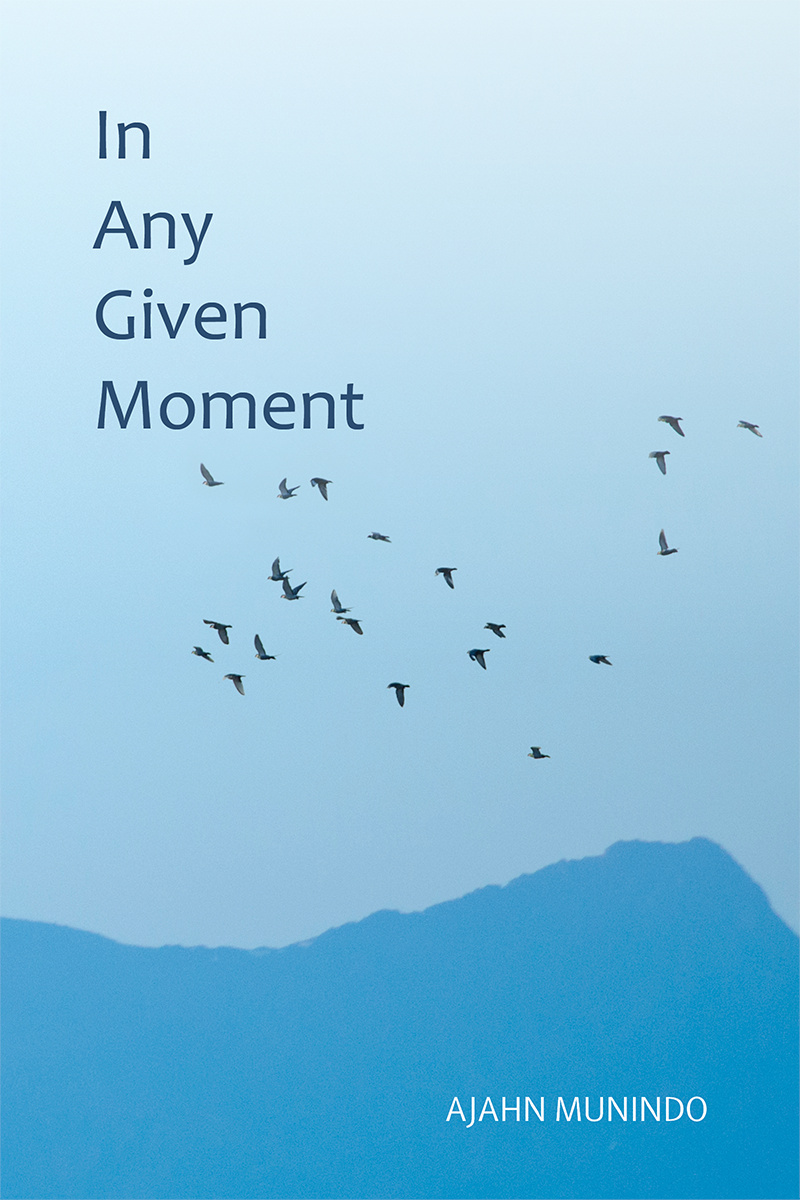
\includegraphics[height=\paperheight]{./desktop-cover.jpg}}
\else

\thispagestyle{empty}
\mbox{}
\pagecolor{frontblue}
\newpage
\thispagestyle{empty}
\nopagecolor
\mbox{}
\newpage

\fi

\cleartorecto
\thispagestyle{empty}

\mbox{}\vfill

\hspace*{5mm}%
\begin{minipage}{\linewidth - 10mm}%
\setlength{\parskip}{5pt}%
\fontsize{10.5}{14.5}\selectfont
\raggedright
\itshape
Gradually, gradually,\\
A moment at a time,\\
The wise remove their own impurities\\
As a goldsmith removes the dross.

\vspace*{\baselineskip}

Dhammapada verse 239
\end{minipage}

\vfill\mbox{}

\cleartorecto
\thispagestyle{empty}
\vspace*{5em}

{\centering

\settowidth{\titleLength}{%
  {\Large\chapterTitleFont\scshape\MakeLowercase{\thetitle}}%
}

{\Large\chapterTitleFont\scshape\MakeLowercase{\thetitle}}\\[0.3\baselineskip]
\setlength{\xheight}{\heightof{X}}
\raisebox{0.5\xheight}{\color[gray]{0.4}\rule{\titleLength}{0.25pt}}\\[0.3\baselineskip]
{\itshape
\thesubtitle}

\vfill

\theauthor

\vspace*{5em}

}



\cleartoverso
\thispagestyle{empty}

{\copyrightsize
% \centering
\setlength{\parindent}{0pt}%
\setlength{\parskip}{0.8\baselineskip}%

\thetitle\\
by \theauthor

This publication is made available\\
for free distribution\\
by Aruno Publications

Aruno Publications is administered by:\\
Harnham Buddhist Monastery Trust\\
Company No. 6688355,\\
Charity Reg. No. 1126476

Contact Aruno Publications at \href{https://ratanagiri.org.uk/}{www.ratanagiri.org.uk}\\
This book is available for free download at\\
\href{https://forestsangha.org/}{www.forestsangha.org}

ISBN \theISBN

Copyright \copyright\ Aruno Publications 2021

\vfill

{\footnotesize

This work is licensed under a Creative Commons\\
Attribution-NonCommercial-NoDerivatives 4.0 International~License.

Produced with the \LaTeX\ typesetting system, set in EB Garamond,\\
Alegreya Sans and Merriweather.

% \ifdesktopversion
% \theDigitalEditionInfo
% \else
% \theEditionInfo\\
% \theDigitalEditionInfo
% \fi
\ifdesktopversion
\textit{\theDigitalEditionInfo}, 2021.
\else
\theEditionInfo\ (\theDigitalEditionInfo)
\fi

}}


\cleartorecto
\tableofcontents*

\chapter{Preface}

This book has been compiled in large part because dwelling on thoughts
of gratitude brings happiness. Also, as I approach seventy years of age,
I find myself drawn to recollecting and reviewing earlier events in my
life and noticing how differently I now feel about them. As the writing
of these notes progressed, it became apparent that, in addition to
gratitude, I have been reflecting on two other themes: the dynamic of
spiritual community and ways of supporting our spiritual life.

The title, `\emph{In Any Given Moment}', means two things to me. One way
of reading it reminds me that in any moment there is the potential to
let go of our painful habits of clinging and consider the larger,
spacious context in which this drama of life is taking place. This is
how I understand, `Going for refuge to the Buddha': trusting that there
is selfless, just-knowing awareness.

\enlargethispage{\baselineskip}

In another way of reading it, the cover image of an open sky (thank you
Chinch) together with the title, suggests that whether or not we notice
the beauty of life in any given moment depends on how present we are for
it. When our faculties are obscured by self-centredness, we risk
becoming lost in memories of the past and fantasies of the future; as a
result our attention readily settles on what we perceive as lacking or
`wrong' with life, and we fail to notice the goodness and beauty right
here in front of us. If our vision begins to clear, if the dross of
unawareness is gradually removed and the gold of awareness revealed, a
thoroughly different perspective might emerge.

The timeline as it is presented here should not be taken too literally.
I have tried to be accurate; however, accuracy over dates and times was
not the main point of the compilation. I apologize if any inaccuracies
or inconsistencies cause confusion. The main point has been to reflect
on gratitude, community and sustaining spiritual practice. These three
themes are the foreground, with the incidents and events of my life as
the background; sometimes the background is not quite in focus.

The significant moments that I reference in these pages, both the
positive and the negative, are moments and events that stand out as
having been helpful in my effort to be freed from the addiction to
self-centredness. By no means have all the positive influences been
mentioned, and definitely I have not included many of the negatives.
Readers will find that the first six parts of the book read somewhat like a travelogue
interspersed with Dhamma reflections. Part seven is almost
entirely Dhamma reflections. It wasn't that I set out to write a book in
this style, it is just that this is how it unfolded. My hope is that
anyone who reads it will discover something beneficial for themselves
and perhaps find something that they want to share.

\bigskip

{\raggedleft
  Ajahn Munindo
\par}



% Page 1 is the first page of the first chapter.
\mainmatter

\part{Taking Shape}

\chapter{The End of the River}

Approximately eight-five miles south of Auckland, in New Zealand's North
Island, there is a small town called Te Awamutu. This is where I was
born in September 1951 and was given the name Keith Morgan. The Maori
name of the town, Te Awamutu, translates into English as \emph{the end
  of the river}. In various online resources\cite{early-history}
it is explained that it wasn't that the river
Manga-o-hoi actually ended there, it was just that beyond that point it
became unnavigable by canoe. I'm guessing that in 1951 the town had a
population of about 5000. The area had a history as a place where
battles had been fought between opposing Maori tribes, where an early
group of Christian missionaries had established itself, and as a
settlement used by the British military during the Waikato wars. By the
time my parents, Pearl and Ian Morgan, moved there, Te Awamutu had found
its identity as a service centre for the surrounding farming
communities.

Christianity was a defining element in our family. My father was the
youngest of six children in a family headed by a Presbyterian minister,
Rev. Richard Morgan and his wife Grace Morgan. My mother was the only
child of a Baptist minister, Rev. Alfred Dewe and his second wife, Sadie
Dewe, or `Nana' as we knew her. Rev. A. Dewe died young and so eventually
Nana remarried another Baptist minister, Rev. Christopher Wilfrid
Duncumb, after spending a number of years as housekeeper to a
Presbyterian minister, Rev. Lloyd Wilkinson. Auntie Nessie, my father's
older sister, was a deaconess in the Presbyterian Church, Uncle Roy was a Baptist
minister and my younger sister, Jennifer, went on to become a pastor,
who, along with her pastor husband Guthrie Boyd, ministered within the
church of the Assembly of God. Recently I found out that my younger
brother Bryan, is ministering these days as a lay preacher in the Paihia
Christian Fellowship.

We lived in Te Awamutu for about two years before moving to a similar
sized town, Morrinsville, about twenty miles away. I imagine my father's
work was the reason for the move. Although for much of my life I have
struggled to find my place in this family, this does not mean I don't
value it. To be born to parents who worked so tirelessly to raise their
four children in a wholesome environment was indeed a blessing. At later
stages in my life it became apparent that growing up in that environment
was a mixed blessing and it did take some skill and discernment to
decipher which aspects were truly valuable and which needed to be left
behind.

When I think back now about my father, I have huge admiration and
gratitude for his integrity and kindness. Besides his Monday to Friday
job working in Hawkes Motors Ford garage, initially as a mechanic and
eventually as the manager, he would spend many hours after work and on
the weekends cultivating a substantial vegetable garden that he had
planted out the back of our house. Always on Sunday he would drive the
family to the morning church service and, for many years, lead the
Sunday school of which he was superintendent. Regularly after Sunday
lunch, he would drive out to remote village halls -- places like Tahuna,
Ngatea, Patetonga -- to conduct a church service for the farming
families who couldn't manage to get into town.

Similar feelings of appreciation arise when I remember my mother's
dedication and how she would spend days on end in the kitchen throughout
the hot summers, bottling and preserving vegetables, apples, and peaches
and pears to keep the family well fed through the year. She also sewed
many of our clothes.

Bible readings and prayers at the evening dinner table were normal. The
summer camp I was sent to was a Christian Youth Camp (CYC) at
Ngaruawahia. Since my parents were teetotal, and drinking at the pub was
a national pastime in New Zealand, we had very few visitors. The only
visitors I remember coming to our house were relatives who were equally
if not more devout Christians, and other families who attended our
church. Devotion to religion from such an early age served to instil
virtues in me which I continue to value. I can't recall my parents ever
arguing and, with only one very minor exception, nor did I ever hear
either of them speaking critically of anyone.

Music was another central aspect of our family life. Both my mother and
father were vocal leaders during hymn singing in church on Sunday; not
just singing loudly, but with fervour and enjoying the opportunity to
break out into harmony. My mother sometimes played the organ in church.
At home, our idea of a good time amounted to us children standing around
singing praise to Jesus while Nana played the piano. Auntie Nessie spent
many years working as a missionary to various Maori communities, and
leading a choir of Maori singers.

David, my older brother by two years, learned to play the cello. I
played the violin for a while, and I seem to remember that Jennifer, my
younger sister, played the piano. Compared with what most families these
days might think of as having a good time, our hymn singing sessions
probably sound rather tame, however I recall them as a source of
considerable happiness: the togetherness, the sheer pleasure of making
beautiful music and the delight in praising the Divine. When I was old
enough to have my own bicycle I would regularly ride out into the
countryside to be alone. I frequented the woodlands along the banks of
the nearby Piako River where I would passionately sing my heart out.
Something about unrestrained adoration of the Almighty triggered
tremendous joy within me: it was thrilling, even electric and
exhilarating.


\chapter{Being Different}

It must have taken considerable effort on the part of my parents to be
so supportive of my evolving character. New Zealanders back then seemed
to proudly present themselves as a nation defined by Rugby, Racing and
Beer. Despite my father's attempts to direct me towards enjoying the
sport, I think I played rugby only twice during all my school years and
remember on one of those occasions kicking the ball in the wrong
direction. Horse racing was associated with gambling, which in the
Morgan household was seen as evil. The mere smell of beer (at that early
stage of my life) was repulsive to me. Walking past a pub and catching a
waft of the hot, stale air that drifted out -- a combination of tobacco,
crisps, beer and Dettol used for cleaning up the vomit -- was a powerful
disincentive. For the duration of most of my early life, laws in New
Zealand required pubs to close at 6 pm. That meant for many that once
work finished at 5 pm, they would rush to their favourite watering hole
and drink crazily for an hour before loading up with an armful of
bottled beer and driving home. When the law changed, pubs were permitted
to stay open until 10 o'clock, but I think the immoderate drinking
habits of Kiwis took longer to change.

The encouragement I received from those who cared for me was a gift --
not only the support given by my parents but also by my Nana. With
hindsight I see now there were strong undercurrents of fear and
judgement around sensuality and pleasure, but I credit both my parents
for daring to allow me to follow my own creative pursuits. It mustn't
have been easy for them considering their own puritanical upbringing and
the pressures that inevitably come with living in a small country town.
Once, when I went to stay on a farm with some friends of our family, the
children there had their bedroom walls lined with awards they had won on
Calf Club Day. Calf Club Day was the occasion when the sons and
daughters of farming families would bring their pet calf or sheep to
school and parade them around the playground and be judged; I'm not sure
what criteria were used for awarding points. I expect I liked it about
as much as I liked the rugby matches that we watched. (Years later I
developed a keenness for watching rugby, but by that time I was tuning
into the spirit of cooperation, even selflessness).

My bedroom walls, on the other hand, were proudly plastered with awards
I had received at the local Flower Show -- a kind of Morrinsville
version of the Chelsea Flower Show. These shows took place three or four
times a year, coinciding with the seasons. Still I can recall the impact
of a wonderfully intoxicating fragrance that hit me when I walked into
the hall where the show was being held. Many of the prizes given out at
the show were for exceptional blooms or for particularly impressive
pieces of fruit or vegetable; the awards I won were for flower
arranging. I am thankful towards my parents for being so daring.


\chapter{Doctor Albert Schweitzer}

Around the age of fourteen I was given a copy of a book, possibly as a
Christmas present, about the French-German philosopher, theologian,
musician, writer and doctor of medicine, Dr.~Albert Schweitzer\cite{schweitzer}.
I'm not sure which came first, the book or
the idea of my entering into the Rotary Club speech contest that ran
each year at our school, Morrinsville College. Whether it was my
parents' idea or mine, I also don't know, but at some stage in my early
teen years I assimilated the idea that I would grow up to become a
preacher. It isn't hard to imagine how such a suggestion might have
become lodged in my mind. Entering that annual contest and speaking
about Dr.~Albert Schweitzer, fitted with that vision. As far as I recall
I made it into the semi-finals or perhaps even the finals of the
competition, but I didn't win. What matters now though was the good
fortune of having been made aware of this extraordinary human being.
Dr.~Schweitzer started out studying for, and achieving, a PhD in philosophy,
then the next year a PhD in theology; he was a world renowned organist,
an expert on and writer about Johann Sebastian Bach, and that was all
prior to studying and graduating as a medical doctor so he could spend
fifty years serving the sick and needy in a remote medical facility in
equatorial Africa. When in 1952 he was awarded the Nobel Peace Prize,
the prize money went straight to the hospital. I feel fortunate to have
been introduced at that formative stage of my life to such an example of
selflessness. There are some who have written critically about
Dr.~Schweitzer, and I am sure he himself would have been critical of his
failings; however the manifest goodness of this man is truly worthy of
admiration.

Many years later when I read and heard talks by the Jungian analyst
Robert Moore, I became aware of the power of intentional admiration. By
consciously admiring a particular quality in another, that quality can
be nourished within ourselves. I have no recollection whether
Dr.~Schweitzer's being a vegetarian impacted on me at the time, but perhaps
it did. His \emph{reverence for life}, as he referred to his commitment
to harmlessness, meant that not only was he vegetarian, but he also
refused to kill insects.
Vegetarianism, and eventually a purely plant-based diet,
became an important part of my life some years later.

\enlargethispage*{\baselineskip}

I think it was also when I was fourteen years old that I contracted
hepatitis. In the summer of that year, probably 1966, as was usual for
our family we had gone away for the holidays. Almost without exception,
every year we would go to a rented cottage (`bach' in Kiwi parlance)
near a beach somewhere, and spend many hours swimming in the sea and
playing in the sand (totally unaware in those days of the risks that
come with excess exposure to UV). That year, we went to Ohope, near
Whakatane. I remember that we were eating a lot of fish at the time and
when I fell ill it was assumed that somehow the fish had given me food
poisoning. It was only once we returned to Morrinsville that my illness
was diagnosed as hepatitis. Horrible as it was, it only meant I was
bedridden for a few weeks and missed some classes at school. One of the
enduring unpleasant memories of that period, however, was being visited
by one of the Sunday school teachers who appeared to me to be there
under duress. I can't say what her intentions were but somehow I didn't
like her visiting me. Possibly by that stage I had already learnt to
pretend to be virtuous in an attempt to win approval, and in the
process, betrayed myself. Maybe I thought I sensed something like that
in her.

\enlargethispage*{\baselineskip}

A few years earlier I had made the mistake of lying to my parents about
giving my heart over to Jesus. I observed how when my older brother
David announced he had made such a commitment to the Lord, he received a
lot of approval and affection. I wanted some of that. Unfortunately, the
importance of impeccability was not something I had learned about so I
wasn't aware of the painful consequences of telling such an untruth. It
was only years later that I began to see how, when we lie, we create a
fissure in our minds which leads to instability. We then compensate for
the feeling of instability by becoming rigid, which obstructs the flow
of life. We turn ourselves into someone untrustworthy: a recipe for
self-hatred and guilt. For fourteen-year-old Keith Morgan, sadly, the
darkness was already beginning to descend.

Auntie Nessie is mentioned several times in these notes, which indicates
the special place she has in my heart. If I had shared with her back
then how badly I felt about the lie I had told my parents, I am sure she
would have listened carefully, looked at me with her kind eyes, and said
something that would have made all the difference. It was generally
understood that Auntie Nessie was a faith healer and I have the
impression that she was held in high regard in various parts of society.
She would never take personal credit for any ability she had, and was
always quick to ascribe all goodness to her Lord. A few years later in
1973 she received an MBE from Her Majesty The Queen, by way of
recognition of the work she had done in Arohata Womens' Prison. One of
the favourite memories I have of her these days is, once when she had
come to stay with us, we children begged her to perform a Maori haka\cite{haka}
for us before we would go to sleep. In
my mind's eye I can still see her standing at our bedroom door, slapping
her knees, with her tongue out and eyes bulging. We loved it and I loved
her. A heartfelt thank you to Auntie Nessie.

When I was about fifteen years old, members of our local church began
discussing the possibility of replacing the church building. With my
parents' encouragement I spent a lot of time producing designs for the
construction. Probably this was the first time I entertained the fantasy
of one day becoming an architect instead of a minister or a missionary.
Over the next few years, however, I discovered that, although I took
considerable pleasure in producing designs, I was utterly hopeless when
it came to mathematics. Working with numbers, and for that matter even
reading books were, and continue to be, a chore (more on that later).
The love of imagining, and sometimes having the good fortune to design
actual buildings, remains with me. It is hard to explain the pleasure I
derive from creating a space in my mind that feels right and then seeing
it manifest in form. As far as I am concerned, successfully designing
living spaces is primarily not about how the space looks, but how it
feels when we are in it. After all, we don't live in the things, we live
in the space. Many people, it seems, don't recognize this, which is
presumably why they fill their living spaces with so many things. They
assume that including yet another nice thing will make the place look
nicer, when in fact that extra thing might well offend the space,
regardless of how attractive the item in itself might have appeared.

As a present on my sixteenth birthday I was given a course of private
art lessons in oil painting by a nationally recognized painter, Violet
Watson. Not that I was any good at painting but I imagine it was better
than pretending I wanted to play rugby. Morrinsville produced several
rugby players who featured in the national All Blacks teams -- Don
Clarke and Ponty Reid are two names that come to mind. On one occasion,
when the All Blacks had done particularly well overseas, the players
were honoured with a procession down the main street, Thames Street.

Already I have mentioned that I learned to play the violin. I can't be
sure now about details, but I think that this lasted for about three
years. The school provided the instrument and the instruction. As I
recall, the music teacher I had at Morrinsville College was very encouraging.
The most enjoyable aspect of it came when I was accepted into the
Waikato Youth Orchestra. Each Friday afternoon after school, I would
hitchhike, carrying a violin, the twenty or so miles to the nearby city
of Hamilton. Being part of that body of people, with a shared fondness
for making music, was a highlight of my week. Many years later, when a
Jungian psychoanalysis friend described spiritual community as `a
harmonious resonance of shared aspiration', I felt like I could get what
she was talking about. Perhaps my time playing in that orchestra helped
with my understanding. After these sessions of practice finished I would
take a train back to Morrinsville.

Thinking back about it now, it surprises me that I didn't feel more
bothered than I did by the fact that I wasn't fitting in with the other
boys. One explanation might be that because our family, for obvious
reasons, was considered churchy and thereby somewhat different, I
perhaps assumed that not fitting in was somehow normal. Children naively
assimilate all sorts of assumptions. Another explanation could be that I
was learning to hone down my skills in self-deception. I was betraying
myself by not truly feeling what I was feeling and as a consequence
gradually becoming more fragmented within.


\chapter{Difficult Lessons}

There was plenty that happened during the nearly fifteen years we lived
at 81 Studholme Street, Morrinsville, that was not particularly pleasant
and that left a strong impression. One of my favourite pastimes in those
days was cycling with a friend to a disused quarry on the edge of town.
For most of the year there was plenty of surface water which meant it
was a great place to collect tadpoles and bring them home to watch as
they turned into frogs. On one occasion a group of other boys were at
the quarry and they were more interested in torturing the tadpoles and
frogs. These days I have an impression of the group setting up our glass
jars in which we had collected the tadpoles and using them for shooting
practice with their BB guns. Another painful impression of that day is
of those boys blowing up frogs using firecrackers. Whether these events
actually took place or not, I can no longer be sure; perhaps they just
spoke about doing it. However, what I do remember vividly, was speaking
to some adults about it, perhaps my parents or grandparents, expecting
them to sympathize with my hurt feelings at what had happened, only to
be disappointed when I found out they seemed to think nothing of it. I
still feel that brutality of any kind, including that done by small boys
against tadpoles and frogs, should be called out. Small barbaric acts
desensitise our hearts and can lead to bigger barbaric acts.

On another occasion I was surprised and disappointed when my
grandfather, Rev. Duncumb, one day took me into the living room in our
house saying he had something that I would like. I imagine he knew that
I was fond of collecting things like bird skeletons and dead spiders. To
my dismay, the thing he wanted to show me -- indeed, I think, give to me
for my collection -- was a handsome moth which he had skewered with a
pin to the back of the sofa. How could a man of God do such a thing?
Obviously I had a lot to learn about life. Thinking about it now, it
might have been that he found the moth already dead and just put it
there for me, but I doubt it. The idea that animals don't have souls,
that only humans have that privilege, is one of the intensely
regrettable aspects of many theistic religions. In my mind, the pain and
distress humans have caused and continue to cause to living beings, on a
mass scale, is one of the reasons why our human family is in such a
tragic state. Every time we intentionally cause harm, the native
kindness and sensitivity of the human heart is obscured. Not only do
other living beings suffer, but we hurt ourselves in the process.
Because we weren't taught this truth, or at least didn't really
understand it, we go on to deny the pain and the loss of self-respect
that we are causing ourselves, and then feel confused by the gradual
sense of deadening and unhappiness that is taking us over.

It should be emphasized at this point that despite the example of my
being shocked at my Grandfather's actions, in no way am I suggesting
that I was beyond wanting to cause harm. One day a friend invited me to
go hunting rabbits with him and I agreed to go along. If I am honest I
think part of me was really excited by the idea. I wasn't consciously
aware at that stage of an inner conflict between very base instinctual
impulses such as wanting to fight and to conquer, and the more refined
impulses human beings have, such as the inclination towards compassion
and humility. On that occasion I did actually shoot a rabbit, however I
only wounded it, which meant that by the time we had reached it, it had
crawled into a wood pile. I felt ashamed. That pain of remorse has
stayed with me. It was similar when we used to go fishing: I liked the
thrill of the challenge, but when it came to seeing the eyes of the fish
as I cut its throat, I struggled. On one occasion at least I recall
refusing to do it, and gave the fish I had caught to my brother. It took
me many years and a lot of effort to even begin to find the right kind
of strength to be able to hold the inner tension between the wild,
unruly animal aspect of our nature, and the love and joy one might feel
towards that which we trust is inherently beautiful, without condemning
the struggle. Now I see such a struggle as inevitable for all those on
the journey of awakening. It is important we understand that we do have
a choice: either we struggle in a way that leads to further struggle, or
we struggle in a way that leads to the end of struggling. If we are
inspired by the latter then we are obliged to train ourselves to
skilfully inhibit the base impulses and cultivate the more refined.
Admitting this is not a form of abdication, it is simply being honest.

When I was given my first camera I was excited at the possibilities it
presented. It turned out, however, that not everyone shared my passion
for photographing toadstools and fungi. It was yet another surprise to
be told I shouldn't be so wasteful and ought to be photographing
sensible things. I guess by that they meant family photos taken after we
had come back from church.

In my sixteenth year Nana died. As with many members of our family it
seems, it was cancer that took her. She was staying in our house at the
time and, although I was asked if I wished to see her corpse and say my
goodbyes, I said I didn't. That was another lie, as I expect I very much
did want to see her. Nana was my favourite member of our family, along
with Dad's sister, Auntie Nessie. The warmth of their hearts had not
been overshadowed by the cold insensitivity which comes with clinging to
dogmas. Sadly, on that occasion my commitment to playing the game was
stronger than the impulse to be honest. I didn't feel able to allow
myself to be seen in my upsetness. After the funeral, when a minister
poked his head through the car window and tried to be helpful by saying
to us children that, `Never mind, Nana has gone to a better place', I
thought the comment worse than pointless. In a way that I probably
couldn't quite define at the time, it felt somehow insulting. He was
trying to be supportive, but as became increasingly obvious to me,
trying to be good is not enough. Without matured and considered empathy
we misjudge situations.

Without mindfulness and empathy we always run the risk of projecting our
own ideas and needs onto others. At a later stage of life, when I came
across some studies on the psychology of fundamentalism, it helped me
make sense of what I have often experienced as insensitivity, even
arrogance, on the part of followers of this or that religion. People of
all religious persuasions, including Buddhists, run the risk of trying
to impose their convictions and preferences onto others. Just because we
find a belief gives rise to good feelings within us personally, does not
mean that belief is ultimately true. Studying a little bit about
fundamentalism helped me see how all unawakened beings are at risk of
compensating for a lack of inner security by clinging to forms; that
includes material forms such as drugs and patterns of behaviour as well
as to beliefs. It would be very useful if a course in the psychology of
fundamentalism were to be taught in schools.

I think it was also in my sixteenth year that I lost all my teeth.
Probably that sounds like a serious thing to happen to such a young man,
and it obviously wasn't insignificant, however I was relieved. I
understand that my mother and grandmother had both lost their teeth when
they were thirteen, and since I was around that age I had been in a
great deal of pain. The dentist wasn't in a hurry to take all my teeth
out, but by sixteen it was obviously the right thing to do. A deformity
of the roots (as far as I recall) meant the teeth were going rotten and
the nerves were being pinched. My teeth looked alright from the outside
but because they were rotten, I was being poisoned. Having dentures at
that age was yet another piece of conditioning that caused me to feel
like I didn't fit in. Somehow, though, I didn't succumb to self pity.
Maybe I even thought I was special. I had been taught to think that
those who believed in Jesus were special. They were saved and would be
going to heaven when they died, whilst those who didn't believe were
headed for a very sorry destination. Another example of arrogance born
out of unwise assumptions.

By that age I think I was already becoming aware of a deep, dark sense
of guilt. However, my inability to acknowledge the extent to which I was
feeling guilty meant that that invidious form of pain was accumulating
in unawareness, generating potential for future confusion. The more I
lied to myself, the more I became divided within myself. Part of what
made it so difficult to own up to was that I didn't really know where
all this pain was coming from. Of course I blamed myself for the most
part. Only many years later was I able to understand how as children we
readily take on our parents' pain in an effort to make those caring for
us appear more competent.

Despite my mother's dedication to caring for all of us, and despite her
fervent love for Jesus, I sense she was fundamentally unhappy. I don't
think she knew how to love herself or be kind to herself. In our family
we never spoke about anything personal -- conversations were always on
the level of what one was supposed to say or feel. At least that is my
reading of it; perhaps my siblings perceived it otherwise. So I am
guessing when I say that I imagine my mother was carrying a huge burden
of guilt for much of her life. I still feel sad when I think of it. How
can people who are trying so hard to be honest, kind and generous end up
being so unhappy? As I found out later when I encountered the Buddhist
teachings, it takes more than goodness, it takes wisdom: it takes wise
reflection to see beyond the way things appear to be to that which is
real. For instance, the idea that it is somehow virtuous to hate
ourselves for having made a mistake, leads to poisoning ourselves, to
self-harming. While aversion is natural, when we make it `my' aversion
through clinging, it turns into hatred and becomes toxic. Guilt is a
distorted form of aversion and manifests as self-hatred, obscuring any
possibility of real contentment. We try to make ourselves feel better by
hating ourselves for having been bad. We are taught that God casts those
who have sinned into eternal hell and that looks like an act of hatred.
So in an attempt to be virtuous, we play God and condemn ourselves for
the things we get wrong. On a level of conditioned thinking this is
sometimes how it works. With wise reflection, however, there is the
possibility of letting go of such wrong thinking and arriving at an
appreciation of what the Buddha said in Dhammapada verse 5,

\enlargethispage{\baselineskip}

\begin{quote}
  Never by hatred is hatred conquered,\\
  but by readiness to love alone.\\
  This is eternal law.\cite{dhammapada}
\end{quote}

Before reflecting on the next stage of this journey, perhaps I could say
something about what I mean when I use the word `wisdom'. In 1975 I was
living in a monastery called Wat Hin Maak Peng, which was perched on the
banks of the Mekong River, just north of Nongkhai in North East
Thailand. My translator at the time reported to me a conversation that
the teacher, Tan Ajahn Thate, had had with his monks. Tan Ajahn Thate
asked the question, `Since the face uses a mirror to see itself, what
does the heart use to see itself?' Apparently none of the monks replied
so Tan AjahnThate answered his own question, saying: `The heart uses
wisdom (\emph{pañña}) to see itself.' Wisdom in this context refers to a
self-reflective capacity within awareness that is activated when other
conditions are sufficiently powerful. At the very least there need to be
the strength and confidence which arise out of integrity, and the
steadiness which is the expression of \emph{samadhi} or well-disciplined
attention. In other words, wisdom is not an accumulation of information;
rather it's a dynamic of awareness that has the function of revealing
the reality of that which appears within awareness. Above I have
mentioned that if we truly wish to be protected from the forces of
delusion, mere goodness is not enough. It requires wisdom.

Now back to the journey.


\chapter{Getting Ready to Leave}

\enlargethispage{\baselineskip}

It was indeed good fortune to have been born into a family that
appreciated the importance of goodness, but when I was seventeen years
old, which was my age in 1969 when we moved from Morrinsville to
Kaikohe, I was completely unaware of the power of wisdom. I was also
unaware of why we were moving. Perhaps it was because of my father's
work or perhaps there were other reasons. He had been given a new job
managing another Ford garage. David had already left home. For me,
Jennifer, and our younger brother Bryan, it was just a case of being
told that this is what was happening: a new town, a new school and of
course a new church.

There are only a few things I remember about Kaikohe since I was there
for less than two years. I do remember that there are thermal hot pools
just outside of the town, called Ngawha Springs. It was worth putting up
with the almost overwhelming stench of rotten eggs for the sake of the
soak in the steaming hot water. I had my driver's license by then and
although I can't be sure, I suspect my mother lent me her car so I could
go out there. At the time I was also hoping that the mud we slopped all
over ourselves would cure my embarrassing acne. Usually I would go there
with a guy called Guthrie whom I had befriended from school. We were
about the same age and went to the same church. These days he is married
to my sister.

That was the year I was admitted to hospital with mumps, meningitis and
suspected pancreatitis. During the school holidays I had gone back to
Morrinsville for a visit and ended up in the intensive care unit of the
nearby Waikato Hospital. The condition was as serious as it sounds and
there were good reasons for putting me into intensive care. As part of
the regime that the doctors put in place to manage this threatening
condition I was on pethidine, which possibly contributed to the fog I
now think of when I try to recall the episode. Thankfully I recovered,
though according to practitioners of traditional Chinese medicine, the
high fevers that go with hepatitis and this latest batch of illnesses,
might have done damage to my kidneys. At the time of writing this I am
nearly seventy years old so the damage mustn't have been too severe.

\enlargethispage{\baselineskip}

As part of the education offered at the college in Kaikohe our class was
taken to visit the nearby Moerewa abattoir. The grotesque sights I
witnessed on that occasion remain etched in my mind. Now I find it takes
effort to register that members of the human race of which I am a part
would choose to conduct themselves in the ways that the workers at that
abattoir did, and probably still do. These days, when the subject of
vegetarianism comes up, I am cautious in what I say since it is easy for
groups of people to become divided according to views on matters such as
diet. I do, however, sometimes subtly suggest that anyone who eats meat
ought to visit an abattoir and see where what they consume comes from
and take on board the implications. The hideousness of the industry, the
harm it inflicts on countless animals, is only part of the story; there
is also the damage the workers are inflicting upon themselves.
Sadly, such conduct has been considered normal for so long that many people
never stop to question it. I believe that for there to be any hope of rescuing
the human race, and planet earth, from the self-destructive trajectory it is on,
it will require a radical transformation of the attitude of entitlement many
humans appear to have. It seems to me not feasible that we can continue to treat
other living beings in such an insensitive and disrespectful manner without
disastrous consequences.

It was also around 1969 that I was introduced to the thinking of the
Canadian philosopher Marshall McLuhan\cite{mcluhan}.
Through the Presbyterian church in Kaikohe I had
become aware of a Christian youth conference to be held in Christchurch
in the South Island. It was on the theme of communication. The poster
announcing the conference quoted from Marshall McLuhan and it piqued my
interest. It said something to the effect, `I am an investigator. I make
probes. I have no fixed position.' This contrasted appealingly with much
of the dogma that, up until that point, I had been obliged to go along
with. So thank you, Marshall McLuhan.

I attended the conference and still recall how inspired I was to learn
about the process of communication. It was pointed out, as I recall,
that communication is not the same thing as expression. We can express
ourselves, but that doesn't mean those who bear witness to our
expression know what we are saying. If we wish to effectively
communicate we need to begin by clarifying for ourselves the message we
intend to get across; then there is the process of encoding that
message, of transmitting the message, receiving the message and finally
decoding it. At any stage in that process there can be disruption
resulting in miscommunication. Whether I read his work at that
conference or later on I am not sure, however I am still influenced by
what Marshall McLuhan had to say in his \emph{The Medium is the
Message}. It was he who coined the term `global village' and readers of
his works these days might be surprised to find how pertinent the points
he makes are in light of our current global crisis.

That period in Kaikohe was the end of my high school education and, once
again, I entered the Rotary speech contest. This time the topic of my
speech was, \emph{Is the purpose of religion to be comforting or
challenging?} I believe I gave a good speech and again reached at least
the semi-finals if not the finals, but the judge scored me down because
I argued the point that religion is supposed to be both: religion ought
to equip us with well-being in order that we can meet the inevitable
challenges of life, or something along those lines. He said my talk
wasn't accurately addressing the topic. Never mind, it gave me some good
experience so that later on when I found myself as the abbot of a
Buddhist monastery I wasn't totally unprepared for speaking in public.



\part{Years of Chaos}

\chapter{Out Into the World}

A vocations advisor I was taken to see during my time at the college in
Kaikohe, recommended me for a job as a trainee laboratory technician in
Holeproof Fabric Mills. I was probably considered suitable because I had
an eye for colours and did reasonably well at chemistry. The job
involved calculating dye formulae by matching small pieces of cloth with
precise colour swatches, and the `recipes' we produced would then be
used in dyeing vast quantities of fabric. So in 1970 I left home and
moved in with the McLean family who we had known in Morrinsville.
Dr.~McLean had moved from Morrinsville to take up a post in a psychiatric
hospital in Auckland and it was conveniently near Holeproof Mills.

One day my attention was drawn to a small book on a shelf in the room in
which I was staying. Maybe it was the title that caught my attention,
I'm not sure. It was a book by Professor Carl Gustav Jung. As I recall,
as soon as I started reading that book I was taken aback by the fact
that he was criticising the Christian church. In my mind the only people
who would openly criticise Christianity were people of no consequence.
Yet here was someone of considerable consequence, a well respected, well
published, world renowned psychoanalyst. This was the first time I felt
I was allowed to start questioning the culture, or even the cult, in
which I had been raised. Thank you very much, Professor Jung and Dr.~McLean.

For the next few years a depressingly dark mood dominated my life. Had I
known then what I know now about depression, I might not have made such
a problem out of it, and, even though I didn't use the word
`depression', I did make a problem out of it. The perceptions of the
world for anyone who is having to endure depression are obviously
negative. However, if instead of demonizing depression and expecting
those suffering from it to get over it, perhaps we could consider it as
a sort of `holding pattern' that is protecting the sufferer from an even
worse state of disintegration. With such a perspective we might be able
to view the condition more creatively, less judgmentally. Because our
society holds up happiness as an indicator of our personal worth, we
readily fail to appreciate the functional value of pain. Not all pain is
pathological. If, for instance, I stub my toe and don't feel any pain, I
won't inspect the wound and see if it is likely to become infected. Pain
can serve a helpful purpose. It says, `Pay attention here.' Besides, the
pain of depression could well be preferable to the much worse
possibility of a psychotic breakdown. During a period of so-called
depression we could be building up strengths such as the self-respect
which comes with cultivating integrity, the confidence associated with
developing mindfulness, and that special kind of nourishment that comes
with cultivating wholesome friendships. Once those strengths are in
place the depression might have served its purpose and dissolve.

Those around me back then didn't seem to notice how despairing I was. I
like to think I was quite successful in acting as if everything was OK.
In my case I would say that put me at an advantage, since if others had
known how negative I felt they would probably have tried to fix me. (I
realize that this doesn't apply to everyone). Sometimes we really need
to endure through the pain of life until we get the message -- and I do
see pain as a message -- which is one of the many reasons why I have
such great faith in the Buddha. At least within the practice of
Theravada Buddhist teachings there is a consistent emphasis on paying
attention to suffering. It doesn't encourage practitioners to dwell too
much on fantasies of possible future states of enlightenment. Many years
later, when a book called \emph{I Am That}, which records teachings by
the Advaita Vedanta teacher Nisargadatta, was popular within our
monastery in England, I read just one, or perhaps two pages, before I
put it down. Not that the content wasn't appealing: it was too
appealing. I was afraid that my mind might start trying to imitate what
the teacher was saying and that would get in the way of making my own
discoveries. This is not to say others shouldn't be reading Nisargadatta and
the like if they find it helpful. People are different and I am one of
those people who likes to find things out for themselves. When we hear about
the realizations of others can indeed be encouraging, however we need to
be careful not to feed on the good feelings that arise out of receiving
such encouragement. Suffering is what we have, what we can know here and
now. Right practice means preparing ourselves so we are ready to
accurately receive suffering when it impacts us, and to see beyond it:
seeing in a way that leads to letting go.


\chapter{Jumping Sundays}

One rare splash of colour that still shows up amidst the memories I have
of that drab period is the `happenings' which were taking place in
Albert Park. This was 1970: London had Hyde Park Corner, San Francisco
had Haight Ashbury, and Auckland had Albert Park. Situated in central
downtown Auckland, between the business district and the Auckland
University campus, this handsome stretch of exquisitely manicured
gardens, massive mature trees and a Victorian band rotunda, provided a
great location for weekend get-togethers. I can't recall now how I heard
about these \emph{Jumping Sundays} as they were called, possibly through
some of the guys working on the dye floor at Holeproof Mills. Several of
them were members of the PYM, (Progressive Youth Movement)\cite{pym}, a radical
anti-Vietnam-war-and-other-things movement that was upsetting the New
Zealand Establishment. I think I was susceptible in those days to
feeling drawn by anything that looked like it might undermine the
society that I was busy blaming for my misery.

There was music, politics and probably early promoters of the
`back-to-the-earth' movement, as well as the Hare Krishnas, and lots of
colour. Thinking about it now, those events did serve as a hint of
potential aliveness, which was helpful. A dreadful sense of darkness and
confusion was building within me. I had sought solace on a couple of
occasions at local churches -- one on Upper Queen's street and another
at Mt Roskill -- but I walked out of them both feeling more
disillusioned than when I went in. It seems that that is what we tend to
do when we feel pushed to our limits: we try things we perceive as
having worked in the past. This time nothing was working, though those
Jumping Sundays did perhaps quicken the spirit of exploration. To me
they seemed to be in sync with what Professor Jung had to say and what
Marshall McLuhan was about. They may not have provided the missing
ingredient for which I was desperately seeking; however, I would say
they were a harbinger of hope.

The Vice President of America, Spiro Agnew, visited Auckland around
then, very likely trying to muster support for their war in Vietnam. He
was successful in garnering support for street demonstrations and
generated a lot of ill-will. I wasn't convinced though that getting
angry at Agnew or America was the solution.

This was also the time of Peter Fonda's movie Easy Rider which
introduced me to the expression `doing your own thing'. In itself those
few words might not sound like much; however, for me that turn of phrase
somehow symbolized the momentum that was gathering within the
counterculture. On many levels, the ways of doing things that had
previously been considered acceptable had had their day. Due in large
part to the power that technology was increasingly making available to
the average person, the old ways were being replaced. Despite all their
might, America never managed to win their war in Vietnam. Man was able
to walk on the moon, but here on earth we weren't managing very well to
get along together.

Earlier I mentioned how I find reading and mathematics challenging. If
that hadn't been the case back then, I might have stayed on at Holeproof
Mills. Now I feel grateful for those difficulties. Of course I wasn't
grateful at the time; I really did want to feel like I fitted in
somewhere.

The despair I felt towards Christianity took me to the point where I
formally took leave from the church. On my Certificate of Confirmation,
issued by the Presbyterian Church of New Zealand, it is written
(presumably by me), `Now on the Monday 6th April 1970 denounce my
membership of the established church of N.Z.' (The word `I' was missing,
and it should have said `renounce'). It seems strange after all these
years that I still have this certificate. I recently found it bundled
with my old school report book and other papers that I believe my mother
gave me on one of my final trips back home. Surely I hadn't given her
that certificate?

For reasons I can't recall I decided to take a trip to visit my uncle,
one of my father's older brothers, who lived about a hundred and fifty
miles south of Auckland, in Taupo\cite{taupo}.
I imagine I was just trying anything to see if something would work. On
the trip back from Taupo to Auckland, something did work. I was
hitchhiking, which was a thoroughly normal way of getting around in
those days, and was picked up by a couple of university students. In the
course of the conversation we were having, I expressed an opinion about
something which prompted one of the guys in the front seat to turn
around and, in a challenging manner, say to me, `Don't you realize that
you have been brainwashed to think that way?' It felt like something hit
me. The next thing that now I can recall was arriving at my brother's
apartment in Hamilton where I was going to stay the night. At some stage
I started writing down my thoughts, and I had a lot to say. They weren't
about aimless confusion or rambling resentments, rather they were
observations. I felt alive again, and there were no drugs involved.

My brother was friendly with the two girls who lived next door, also
university students, and somehow we met up and I shared with them my
mood of inspiration. They suggested instead of using the word
`brainwashed' I could try using `conditioned'. That fitted. Just the
suggestion that thinking was a conditioned process, seemed to release in
me a lot of energy. At least that is how I now perceive what happened. I
wrote and I sang, in particular I sang along with a record of a song
called \emph{Look Through My Window} by The Mamas and the Papas. What
inspired me were the words, `\ldots{} and I know I should let go\ldots{}'.
Looking online\cite{window} now I see the other words of that song were not
particularly important, it was `\ldots{} and I know I should let
go\ldots{}' that rang true. I sang my heart out as I had
previously sung hymns alone by the river near Morrinsville. Those words
resonated within in a way that felt intensely relevant. A big thank you
to those university students and to the Mamas and the Papas.

Thank you also to Leonard Cohen. There was a poster on the wall in the
living room of those two girls with the words of a Leonard Cohen song.
What a gift. It puzzles me how some people would find his music
depressing. Yes, melancholic, but so beautiful. Many years later when a
friend who was a personal acquaintance of Leonard Cohen's, gave me a
copy of one of his books, he had signed it and added the note `to Ajahn
Munindo with a deep bow'. There was an embossed circular imprint
on one of the front pages which said `Order of the United Heart'. I feel
as if in 1970, on that trip back from Taupo, my heart started on the
journey towards unity.


\chapter{Lifelines}

Around 1971 I enrolled to study psychology, sociology and education at
Waikato University in Hamilton. Choosing that university had nothing to
do with my brother David living in Hamilton -- he and I had never been
close. Perhaps it did have something to do with my having heard Waikato
University had a psychology department that favoured a Humanistic
approach. I had felt encouraged after hearing a bit about Gestalt
therapy which made it seem a more practical approach than that of the
Behaviourists.

Early on, after enrolling at the university, as a result of an
unexpected turn of events, I had met Professor Jim Ritchie who invited
me to join in with a regular extra-curricular sensory awareness group
that met at his house on Wednesday nights. I wasn't totally unfamiliar
with the theory of sensory awareness exercises and encounter groups, but
I had no experience of them. We were a group of about eight to ten,
mostly students at the university with perhaps some ex-students, and we
would experiment with techniques employed in Gestalt therapy. I suspect
those meetings contributed significantly to my beginning to find that I
had my own voice: I had my own desires and opinions. Prior to that, the
conventional sense of who I was had been moulded into a virtual human
being: I said what I thought I was supposed to say and did what I
thought I was supposed to do. In today's language it would be said that
I was totally inauthentic. No wonder I felt so confused. I had no
dependable frame of reference.

Although it is a digression, perhaps at this point I could say something
about what I mean by `the conventional sense of who I was' or about how
I understand `self'. In Buddhist teachings we hear a lot about not-self,
and all of the world's major religions emphasize `selflessness'.
Contrasting that, in the world of psychotherapy, and perhaps especially
so within Gestalt Therapy, there is a strong emphasis on developing
`self'. On the surface these contrasting perspectives could appear to be
in conflict, however, if we look deeper there need be no problem. If we
can appreciate the self-structure (or the ego or the personality) as
predictable patterns of mental and emotional activity that give an
individual a fulcrum or a frame of reference by way of which they can
relate to the world, then we can appreciate its relative function. The
problems arise when we take this structure as ultimate or as permanent
-- as who and what we are: we identify \emph{as} it. In the early stages
of life, if all goes well enough, a conventional sense of a separate
self is configured in an individual and they get on with the various
physical, mental, emotional and relational aspects of their life,
hopefully without too much trouble. That doesn't mean they won't
struggle with the normal suffering of loss, of disappointment, and
eventually of death that life gives us all; addressing those issues is
the domain of a deeper dimension: what we might call the spiritual life.
Real difficulties do appear if during the early stages of life things
don't go well enough, and if the child experiences more distress than
they are ready to handle. What psychotherapists can potentially do well
is to help someone who finds themselves with such unacknowledged
difficulties to come to terms with their past conditioning. A skilled
therapist can help the individual reach a stage of having a well enough
integrated sense of individuality, or self. From that stage onward, they
will be better prepared to deal with the vicissitudes of life. Also,
they will be more ready to take on the tasks of the spiritual journey --
that is, cultivating selflessness. The cultivation of selflessness means
learning to truly see that the self is not-self -- it is not ultimate:
what we refer to as the self, is activity taking place within a larger
context.

Now back to Hamilton.

Jim, as I came to know him, had a holiday property at Whale Bay, near
Raglan. He and his wife Jane and their children would often spend time
there. Also some of the Wednesday group spent time there. Whether it was
with them or on some other occasion, I have a strong memory of one day
noticing a poster on the wall in one of the cabins on that property. All
I recall of the poster was the word printed large, \textls{AWARENESS}. Perhaps
the text under it gave some extra meaning to the word, however, this was
one of those significant moments when something registered: this
mattered. There is awareness. I can't say what it was about that moment
that meant so much, but nearly 50 years later, I am still able to
visualise that word on that poster and recall the moment -- so thank
you, Jim Ritchie.

Jim had a wide circle of friends. He and Jane were well known for their
work studying child-rearing patterns in New Zealand. Also he was close
to some of the local Maori communities and worked hard to get them
recognition. One day when I was at his house, James (Hemi) Baxter turned
up and I can recall the two of them rolling around the living room floor
hugging and playing like two small boys. James Baxter was one of the
best known and most highly regarded poets of New Zealand. He had made
the unconventional choice of living in a commune called Jerusalem, near
Whanganui.

During this period in Hamilton I was offered three lifelines. The first
came from a friend, Jim Smith. Jim Smith and I had met before I came
down to Hamilton and he was also studying at Waikato University. He had
a child to support and I remember helping him one evening (maybe more)
on a night job he had as a cleaner in a school. He gave me my first
Buddhist book: \emph{The Way of Zen} by Alan Watts. What a gift! Here
was a spiritual teaching that honoured the heart's yearning for insight
into that which matters most in life, and it didn't demand naive
acquiescence. There was one phrase from that book that stood out for me;
as I recall it was presented as a summary of Zen Buddhist teachings. It
said something to the effect, `When you sit just sit; when you walk just
walk; above all don't wobble!' Although it was already quite late at
night when I read that, I was so inspired I simply got up and went
walking around the streets of Hamilton. Of course I was thoroughly
wobbly, not just when I was sitting or walking, but here was another
hint of a useful direction in which I could be seeking.

It might also have been Jim Smith who gave me a book by Krishnamurti.
There was a Krishnamurti Society at our university but for some reason I
was not drawn to it. What I did value though was reading in one of
Krishnamurti's books where he made the observation that most people
assume gratification of desire and satisfaction are the same thing, when
they are not. I don't know what else he said. I suspect I didn't read
more than the first page, but that much was helpful and has stayed with
me. It fits with so many other teachings I have received over the years,
including of course, teachings by Tan Ajahn Chah. With gratification we
get momentary relief from the pain that arises from being caught up in
wanting, being identified with wanting. True satisfaction is what arises
in those who have let go of all identification with the movement of
wanting. They know, and can wisely and compassionately accord with, the
reality of wanting.

Although I have said reading was challenging, now that I think of it
there were a few books that I found nourishing. RD Laing's \emph{Sanity,
Madness and the Family}, which I probably had to read as part of the
psychology course, also his, \emph{The Divided Self}, and \emph{Knots};
Alan Watts' \emph{The Taboo Against Knowing Who You Are}; Paul Reps'
\emph{Zen Flesh, Zen Bones}, and his \emph{Square Sun, Square Moon}.
None of these came close to giving me the missing ingredient, however
they did provide a bit of colour at a time when my life was painfully
grey.

Music was also providing some colour, however these days I struggle to
remember much of what I was listening to. I can however fondly recall
\emph{The Incredible String Band} and in particular their song about
water. One line I am happy to still have floating around in my head,
`Wizard of changes teach me the lesson of flowing.'

The second precious lifeline thrown my way came from a Canadian woman,
Lynn, whom I knew from the Wednesday group meetings at Jim Ritchie's
place. She generously paid for me to receive initiation into
Transcendental Meditation. It might in fact have been her partner David
who paid, I'm unsure. TM represented something to me. I don't know if
the mantra I was given was genuine or something that the business-like
gentleman who gave it to me had just made up. I confess that I failed to
abide by all the `terms of use' prescribed for TM meditators, and from
time to time I continued to indulge in various forms of unwholesomeness.
Nevertheless, it represented and introduced me to the discipline of
attention. Thank you very much, Lynn and David.
I cannot possibly estimate the value of that introduction to the world of meditation.
These days Lynn and I are still in
contact, although usually only once a year. She has been a dear Dhamma
friend.

Just before the beginning of my second year at university I joined a
group of about a dozen other friends and acquaintances in moving to live
in a couple of houses on a farm near Gordonton, a few miles outside of
Hamilton. It is hard to define what it was that drew us together,
probably a shared longing for something meaningful, something new. My
sociology lecturer and his wife and children were part of the
`experiment'. Also there was a super liberal Anglican minister who had
previously run a communal house in Hamilton. Raewyn was my best friend
there and she worked in town as a secretary. It is probably safe to say
that most of us were influenced by the book The Greening of America\cite{greening}
and maybe by The Whole Earth Catalogue\cite{earth}.
We were looking towards communal living, I expect, as a solution to the sense of there being something
missing -- what I have been referring to as the missing ingredient.

\enlargethispage{\baselineskip}

Around this time the New Zealand Government was experimenting with what
was called \emph{Ohu}\cite{ohu}, a Maori word having to do with community activities. James
(Hemi) Baxter had become somewhat of an inspiration for communal living in New
Zealand, and this wasn't long after Woodstock had happened in America.
In Nimbin, New South Wales, Australia, they had their own version of
Woodstock. However, communal living in Gordonton didn't turn out to be
much fun. As far as the lecturer and his wife were concerned there
needed to be standards kept that were suitable for raising children.
Some of our group could probably have been described as anarchists. I
naively spoke in praise of Mao Tse Tung (though I knew nothing about him
or the horror he was inflicting on his country). Essentially I was
hoping that if we could live communally all society's problems would be
manageable.

I regret speaking in praise of Mao but I don't feel overly judgemental
of the naivete. How could it have been otherwise? It would have been
better if we had had a modicum of humility, but we didn't. We felt
frustrated and desperate to do something, anything. I had converted the
hen house into my accommodation and was energized by fantasies of the
study of psychology at university and finding meaning in communal
living. Unfortunately, as far as I was concerned, the dominant mood in
that commune was one of desperation.

Before long, disillusionment also set in regarding what was really on
offer at university, combined with the difficulties I was having keeping
up with the reading expected of me, which led to my dropping out at the
end of the first term of the second year. That was Easter, and in New
Zealand by that time winter was rapidly approaching. Raewyn and I
decided we would go to Christchurch for the Easter weekend.

\enlargethispage{\baselineskip}

A few weeks after returning from that trip, it was on Raewyn's motorbike
that I was riding when I had a serious accident. That morning when I
borrowed her bike to ride into Hamilton without a crash helmet and
without a license was to impact the rest of my life. Although it was
around the middle of the day, the conditions were very foggy; the
country road was narrow so I took the liberty of riding nearer the
centre of the road than I should have. I had my lights on, but when I
cut through an `S' bend I ploughed into a car coming in the opposite
direction. The next thing I remember was regaining consciousness on my
way into the operating theatre.

On the negative side of things, most immediately it meant that I spent
quite a long time in hospital recovering from the damage done to my
head, shoulder and ankle, and it resulted in many months of having a
full length plaster cast on my right leg. My parents, as you would
imagine, were not delighted when they heard I had dropped out of
university, but were relieved I hadn't been killed in what was a serious
motorbike accident. Raewyn's bike was a write-off; my lovely hen house
accommodation had to be abandoned as it wasn't suitable for the winter;
the insurance company of the person whose car I hit sued me and it took
nearly all the money I received in sickness benefit to pay that off.

\enlargethispage{\baselineskip}

On the positive side, I received another lifeline. A few months earlier,
at an encounter group-style gathering at Whale Bay that Jim Ritchie had
instigated, I had met an Australian guy, also called Jim, who was currently
living on a commune near Mullumbimby in northern New South Wales. While
I was laid up in bed recuperating I received a copy of a book from Jim
and a mutual friend Roselberry: it was \emph{Be Here Now}, by Ram Dass.
This wasn't just a gift -- it was a treasure. Ram Dass was someone with
bright eyes and a beautiful smile, talking about meditation,
macrobiotics, chanting, pranayama, yoga and spiritual community. True,
he had a strange name and wore robes, but when I read his words they
were like music, beautiful music.


\chapter{Journeying}

There is so much to thank Ram Dass for that I hardly know where to
start. The inspiration I received from that book was likely one of the
forces that motivated my leaving the Gordonton commune.

A few weeks before leaving, at an annual festival of devotion to
Dionysus -- AKA, Auckland University Arts Festival -- I had met an Arts
student from Wellington, John Vincent. We must have exchanged addresses
because when I was in Wellington a few weeks later I looked him up. This
was shortly before my 21st birthday. John was living in a typical (for
Wellington) wooden house in Tasman street, just across the road from
Wellington Polytechnic College where he was doing a course in graphic
design. Nearly all old buildings in Wellington are made of wood because
the city is located on a fault line and regularly receives earthquakes.
(New Zealand has approx. 20,000 quakes\cite{quakes} each year.)
There were five or six friends sharing the place and John kindly invited
me to stay. The house had two storeys (actually, it was two separate
apartments) and we lived downstairs.

Around that time, the government stopped providing me with sickness
benefit money and instead offered me a job, which I was more or less
obliged to take, working as a clerk in the Education Department of the
NZ Government. The only interesting aspect of the job was that it was
housed in the second largest wooden building\cite{building} in the world (at that time).
Architecturally it was glorious. Occupationally it was tedious.

Many interesting things did happen though at Tasman Street. The occasion
which shines brightest in my memory is meeting Jutta Passler. One
evening, during a get-together upstairs, one of the girls who lived
there returned home from an event with a German woman she had met. It
was Jutta. As soon as we were introduced we started talking, almost as
if we already knew each other. It turned out that we had both been at
the same encounter group weekend a few months earlier. It was a weekend
being run by two good friends of mine, Dr.~Jack Prichard and Helen
Merriman, and as I happened to be visiting them at the time, they had
taken me along. The conversation with Jutta that started that evening
lasted for decades. Often I would visit her in Palmerston North where
she was teaching French and German at the High School. Only some time
later did I discover how thoroughly out of character it was for her to
have me stay in her apartment. She was about 20 years older than I and
lived an intensely private life. Her neighbours probably thought her
eccentric.

When Jutta was 18 years old she had been living in Dresden. It was the
time of the horrendous firebombing\cite{firebombing}.
Her mother had died in 1939 because penicillin wasn't
available in those days to the public. Her father had little time for
her so, for a period during her teen years, she had been homeless. In
1945 she had found a place to stay at a girls' hostel. During the day
she was obliged to work at a factory and at night she would regularly
help out at the railway station where large numbers of refugees were
accumulating. They were fleeing from the Russians who were approaching
from the north. On the thirteenth February, 1945, Jutta was staying at
the hostel and had telephoned a friend to say she wouldn't be helping
out at the station that evening. It was that evening that the bombing
began, and along with the other girls, she hid in the basement. At one
stage she came up to look outside but then the second wave of bombings
began. In a record of her life that Jutta shared with me, she says that
as many as 120,000 people were killed. I don't know how that accords
with what was officially stated. The shock was indescribable.

She managed to survive the terror of those nights of bombing and then
she had to somehow survive the hell of the aftermath. It doesn't take a
lot to imagine how life might be for an 18 years old German girl when
she encountered the invading Russian soldiers. Many years later when she
shared her story with me I could see how skilfully she had turned her
struggles into great strength and great integrity.

After the war Jutta moved to live in Paris where she worked as a
housekeeper for an American family. Later on they helped her move to
live in California. Having obtained her Master's degree she went on to
live in Honolulu where she taught at the University, and then
eventually, to New Zealand where she settled. On three different
occasions over those years she met pilots who had flown in bomber planes
during those Dresden raids. Jutta didn't really mind if others thought
her eccentric; she was interested not just in surviving, but in truly
living. She was her own person. I am very, very grateful to have had
such a fine friend. It was Jutta who introduced me to Macrobiotics,
Martin Buber, Meister Eckhart, Constant Comment Tea, and Yellow Red
incense -- the latter still being burned today in the Dhamma Hall here
in our monastery in Northumberland.

When Jutta discussed the topic of authentic being she often used the
phrase, `the bigger the front, the bigger the back', an expression she
said she had learned from Macrobiotics, a discipline which focuses
primarily on food but that aims at finding balance in everything. The
expression refers to people who put up a big front in an attempt to hide
something they haven't yet learnt how to fully receive. It reminds me of
an expression I believe is attributed to Prof.~C.G. Jung, `The greater
the radiance, the bigger the shadow.' Jutta had suffered terribly, but
resolutely refused to play the victim. She wasn't into playing games.
She wasn't into putting up fronts. Several years later I was happy when
she visited me in Northeast Thailand and had an opportunity to meet Tan
Ajahn Chah. He called her Toyota.

Now back to Wellington.

There was one occasion when I spontaneously took off to visit an actor I
had met, Simon, who had a job manning a fire lookout tower on
Rainbow Mountain\cite{rainbow}, near Rotorua. The only thing they expected of him
was throughout the day to keep an eye out for fires in the surrounding
forests. If he saw anything suspicious he had to call it in using the
radio. Simon was an actor but was also writing plays. Being a
fire-watcher seemed to suit him. During my visit there I came around to
fancying myself perched up high in such a tower with nothing much to do
all day long, so Simon set up a meeting with the Overseer. On the day I
left to hitchhike back to Wellington, I met the Overseer at the base of
Rainbow Mountain and we discussed possibilities. I let him know I was
interested but he didn't appear convinced I would make a good fit. He
was right: I was attempting to put up another front. What I needed in
fact was community.

My job doing accounts in the Education Department didn't last long;
instead I took another job driving a delivery van for a pharmaceutical
company. Several of us from the house in Tasman street moved to a place
in Owen street, near the zoo. I managed to get three months free rent
since the previous occupants had left the place in such a filthy
condition. The owner said they planned to eventually knock the house
down anyway so we could be creative in renovating it. (That is how I
interpreted what he said.)

Again it was a wonderful wooden house and this time it had generously
high ceilings, at least by our standards. John lived out the back in
what might have been the old servants quarters, Sally baked excellent
cookies, Rob had an amazing sound system, Andrew was just a really sweet
guy, and Jude was the intelligent one. I had a lot of fun stripping back
some of the walls exposing the wooden panelling, painting other walls,
constructing a kitchen and designing a playroom in which there was an
open fire. It was almost too good to be true. We were a harmonious bunch
and appreciated each other's company. This was the time of \emph{The Yes
Album, Emerson Lake and Palmer, To Our Children's Children's Children,}
and \emph{Ziggy Stardust}.

John spent his time painting and drawing and sculpting. He is one of two
people from that period with whom I have stayed in touch. Our lives went
in different directions but there seems to be something we recognise in
each other. Somewhere around 1977 or `78 he turned up in Thailand. Ajahn
Pasanno and I both happened to be in Bangkok for some reason and were at
Wat Boworn when one day John, or Bodhi as he was to be known, suddenly
burst in. Clothed all in red, he had aligned himself with Rajneesh and
was on his way to Poona in India. I have no idea how he knew where to
find me though I am glad he did. These days I think he has an Advaita
Vedanta teacher. Such friendships are precious. Thank you, Bodhi.

The second person from that period with whom I am still in touch, is Rob
Green. In 1971 he was making money working on the Inter-Island ferry
service between Wellington and Picton in the South Island. Curiously, in
June 1980, almost as soon as I arrived at Cittaviveka Monastery in
England, I received an unexpected phone call from Rob. He was taking
part in a study program in a Tibetan Buddhist Institute in Britain. He
happened to be there when Tan Ajahn Chah visited in 1979. These days Rob
lives in Russia with his partner, and teaches English and we write from
time to time.

My life was taking on a very different shape due to the influence of
Jutta and Ram Dass. I suspect it was through Jutta that I was introduced
to books written by Hermann Hesse: \emph{Narcissus and Goldmund, Demian}
and \emph{Siddhartha}. The spirit of what he wrote was again congruent
with what Prof.~C.G. Jung and Marshall McLuhan had to say. Apparently in
real life Professor Jung and Hermann Hesse were close companions.
Already while living at Tasman street I had started attending hatha yoga
classes at a Centre in Aro Street. This helped get my damaged body back
into working order. Maybe it was through that Centre that I also found
out about a Mantra yoga group in which I began to participate. Having
been inspired by Jutta's dedication to Macrobiotics, my breakfast in
those days consisted of a bowl of plain boiled brown rice with some
super healthy (unsweetened) home-made marmalade stirred in. My
meditation practice, however, was sadly lacking in discipline; I was
very restless.

One day, on the spur of a moment, I caught the ferry from Wellington
down to Christchurch. I wanted to spend time with a fellow I had met at
a music festival in Whanganui, John Britten\cite{britten}.
The culture in New Zealand, at least back
then, allowed for spontaneously turning up at someone's house totally
unannounced. My visit coincided with his taking a trip down the coast to
deliver a car to a friend, so I joined him. John had a way with
vehicles; not only did what he had built run well, his work was
gorgeous. For instance he had converted an old truck into a stunningly
beautiful caravan/mobile home, lined with kauri wood. It was a
masterpiece. He was a character full of creative enthusiasm. Years
later, by which time I was already the abbot at Aruna Ratanagiri, I
reached out to reconnect, only to discover he had died shortly before my
letter arrived. It was then that I found out about how he had gone on to
create a world-famous handmade motorbike that achieved recognition at
Daytona\cite{daytona} and other racing competitions.

Back in Wellington I was beginning to have fantasies of setting up a
pancake shop. This was not about serving delicate dainties sprinkled
with icing sugar: what I had in mind would be made of wholemeal flour
and more likely to be served sprinkled with alfalfa sprouts. The idea
never got much traction. One night several of us went to a Ravi Shankar
concert and met up afterwards with friends and discussed the possibility
of such a shop, but the idea stopped there. What was great though about
that particular evening (besides Ravi Shankar) was that those friends
had just acquired a copy of the newly released Pink Floyd album,
\emph{Dark Side Of The Moon}.


\chapter{Ready to Leave, Again}

\enlargethispage{\baselineskip}

For all the fun we were having, there was still something really
important missing. I felt far from contented. At some point Andrew (from
Owen street) and I hatched a plan to escape to Sydney. Whether Andrew
saw it as an escape or not, I am not sure; he might have had other
motivations. In my case, ongoing indulgence in heedlessness was
undermining my confidence, and, perhaps similar to the way I left
Auckland and left Hamilton, I now wanted to leave New Zealand.

Before departing I visited my parents who lived almost at the other end
of the North Island near the Bay of Islands. After my father had a heart
attack he had left his job managing the Ford garage and they went into
semi-retirement running the General Store at the small seaside village
called Opua. Opua was known internationally as a safe deep harbour where
ocean-going yachts could conveniently moor long term. On one of my
earlier visits to my parents, Green Peace's Rainbow Warrior had been
moored there in preparation for one of their trips to Mururoa Atoll to
protest against France's testing of atomic weapons. Nobody knew at that
time that in 1985 the French secret service would bomb and sink the
Rainbow Warrior\cite{rainbow} while it was moored in Auckland Harbour.

\enlargethispage{\baselineskip}

I suspect that by now my parents had started to accept that I was going
to keep behaving in ways they didn't understand. They still loved me,
but there was almost no real communication between us. My visit home was
not because I actually wished to see them; presumably I felt it was the
right thing to do. That trip north also gave me a chance to say goodbye
to a local potter, Peter Yeates, whose company I had enjoyed in the
past. At the time he was collaborating with the artist Friedensreich
Hundertwasser. Originally from Austria, Hundertwasser was well known,
amongst other things, for his posters advertising the
1972 Munich Olympic Games\cite{olympic}.
In that part of New Zealand he was known for designing the extraordinary
public toilets in Kawakawa\cite{toilets}.

Also, while I was up north, I took the opportunity to visit another
commune I had heard about. It was situated not far away on the other
side of the island at Waiotemarama, near the Hokianga Harbour. The
commune had the rather grand name of \emph{The Foundation of Mankind}. I
managed to get a ride over there on the back of a motorbike and was
pleased I had the chance to see it. There was energy and enthusiasm,
though, thinking back about it now, I suspect they too were finding
communal living not quite as heavenly as they had hoped. As Ajahn
Sumedho has said, ideals are like stars, they are useful for getting
your bearings, but it is not wise to expect to actually reach the stars.
Ideals are also a good way of generating energy, but if we hold them too
tightly, we will end up very disappointed.


\chapter{A Very Foreign Country}

Andrew and I arrived in Sydney, Australia, shortly before my twenty-second
birthday, September 1973. One of the first impressions I had was one of
being shocked at the sight of police in Sydney's airport carrying lethal
weapons. The only real guns I had seen were for hunting rabbits or wild
pigs; in New Zealand the police did not carry lethal weapons.

When we are shocked by something (and I don't mean merely surprised) it
is a sign a bubble we were living in has just burst. The bubble I had
been living in was the idea that the rest of the world was some sort of
slight variation on New Zealand. Unconsciously I assumed everywhere
would be as peaceful and parochial as New Zealand. Although I guess I
wasn't aware we were parochial. Of course I had seen people-killing guns
in movies and on television but only now realized that there are places
where these guns are actually used. Eight or nine months later, another
bubble would be burst when I flew from Darwin in the Northern
Territories of Australia and arrived in what was then Portuguese Timor.

Besides feeling somewhat shocked at the airport I imagine I felt excited
to be somewhere genuinely new. Not long before taking leave of New
Zealand we had hosted a fellow, I think Canadian, at our place in Owen
Street. He must have given us the address of where he expected to be
staying in Sydney since, even though the address was a bit vague, we
easily located the place and found ourselves being received at their
apartment. An American guy called Bill Hamilton was part of the group
living there and he mentioned that we could probably find work at the
Darling Harbour Railway Station. He had a cushy job there spending much
of the day folding tarpaulins. As it happened, I did get a job there
without any difficulty; however, mine was loading beer kegs onto railway
carriages.

Within a few days Andrew and I had found our own place to live in the
suburb of Coogee (which is the Aboriginal word for `stinky', because
large quantities of stinky seaweed sometimes wash up on the beach
there). Also, soon after we arrived in Sydney, an Australian fellow
called John, took me to visit a Buddhist monastery, Wat Buddharangsee,
in the suburb of Roselands. Maybe when we were staying in Bill
Hamilton's place, I had mentioned that I was interested in meditation
and John had picked up on that. Meeting Buddhist monks for the first
time was intensely intimidating. I imagined they would be able to read
my mind and see what a fake I was. I suspect part of me really did want to be seen, but there was also a big part of me that felt like I couldn't handle it. On that
occasion I had the good fortune of meeting Luang Por Mahasamai who
was Laotian by birth but had received his monastic education in
Thailand. He had a big scar across his face that you couldn't help but notice; he also had an even bigger and warm smile. That was the only time I visited Wat Buddharangsee until about five years later.

The next few months were spent accumulating funds so that I could
travel north and join Jim and Roselberry on their commune near
Mullumbimby. On one occasion when working at Darling Harbour Station
there was another of those moments that stood out as significant. In
truth I can't say that the moment stood out at the time: it was only
later that I appreciated how something valuable had been triggered. What
was quickened in me was an appreciation for inner work: psychological
and spiritual work. Of course the concept of doing your inner work was
not new to me, but on this occasion something clicked and a sense of the
significance of being committed to doing your inner work took on new
meaning. The person I was assigned to work with that day was mumbling
and grumbling about something that had upset him until he suddenly
caught himself and said words to the effect, `I have to be more careful.
I had forgotten that in situations when I feel let down by the tools
that I am using, I easily overreact'. It was just that example of
self-awareness that struck me. According to the conditioning I had
received, the only things that really mattered in life were what you
believed. If you professed to believe in the right things then all would
be well, and if you believed in the wrong things then all would not be
well. Although I would not have been able to articulate it at the time,
now I see how that observation usefully brought into relief the lazy
attitude that can become established in our minds if in our early
education we fail to receive wise instruction. Although I can't recall
the name of my co-worker that day at Darling Harbour Railway Station,
thank you.

When later on I became familiar with instructions offered by the Buddha
I began to internalise faith in the law of kamma. It is not the case
that anyone else can take responsibility for our actions; we alone carry
that responsibility. The Buddha rarely criticized other religions but he
was critical of teachings that undermine confidence in the law of kamma.
What he endorsed was what he called \emph{citta bhavana}, or cultivation
of the heart, cultivation of awareness: doing our inner work.

After a few months in Sydney I packed my belongings into a backpack and
headed north. I forget now how I travelled to Mullumbimby, probably by
train, but arriving there felt like how I imagine Muslims must feel when
they arrive at Mecca, or Christians when they go to Jerusalem.

Roselberry had told me to make my way to The Sunflower Cafe and ask for
directions to the Narada commune, which I did. I seem to recall the intensity of emotions
I was feeling was dizzying: joy at seeing beautiful, colourful,
long-haired, bearded members of the back-to-the-earth community mingling
with the local population; along with hope that perhaps I was about to
find a place where I might fit in, mixed with the fear that it might not
work out. A potent cocktail of expectation.

The image I have now of The Sunflower Cafe is that it was full of the
fragrance of patchouli oil, beautiful smiling men, women and children,
bright colours, stained glass, shelves filled with organic produce,
pottery, hand-woven shawls, and walls displaying artwork for sale. The
folk working there helpfully pointed me in the direction I needed to go
to reach Upper Main Arm where I would find the Narada commune.

It puzzles me that I can remember almost nothing about my arrival at
Narada, but this was my first experience of the Australian countryside,
and probably the sun, the heady aroma of the eucalyptus trees, combined
with the sounds of the otherworldly wildlife, all were somewhat
overwhelming. I do however have an impression that Jim and Roselberry
might have given the community members an exaggerated report of me since
they welcomed me almost like family.

There were five or six couples on the commune which comprised
approximately 200 acres of undulating land. It had previously been
farmland but was now covered in lush, subtropical, secondary growth,
mostly varieties of eucalyptus with dense undergrowth of lantana. Mount
Warning was not far away to the north and there was a stream that
meandered along one boundary of the property. Except for a couple who
lived in the main communal house near the entrance, all the others had
their own portion of the property that they occupied and their own
residences. All were Australian, several from Melbourne, some
ex-teachers and others artists, and most had known each other for quite
some time. Clearly they were embracing ideals of cooperative living, but
there was also a decent dose of common sense. For instance, each member
of the commune held shares in the company that owned the property. It
wasn't automatically assumed that I would be invited to live there but
they went out of their way to include me in activities. I wasn't treated
like an itinerant visitor.

The thing that took time and considerable effort to accommodate was the
unfamiliar wildlife. The screaming kookaburras weren't any trouble, they were
fascinating; it was the snakes, the goannas, stinging ants, poisonous
spiders, leeches and ticks that got to me. New Zealand bush, by
comparison, is totally benign. In New Zealand you can walk out into the
bush, pitch a tent and lie down almost anywhere without any bother
(other than from sandflies). I was used to camping and roughing it a
bit, at least that is what I thought, but here, in this very foreign
land, there was always something trying to sting me or bite me. Many of
the creatures and critters were deadly poisonous!

Jim took me to a location a short distance further along the ridge from where he
and Roselberry lived and said it would be alright if I wanted to
construct a small residence there. From that ridge it was possible to
look down the Upper Main Arm Valley over Byron Bay to the ocean. I had
brought a modest sized tent with me, so over the next few days, using
canvas, bamboo, plastic sheeting and a variety of posts and poles, I
constructed myself a dwelling. This was to be my home for the next few
months.

Life at Narada was a mixture of fun and hard physical labour. The hard
labour in my case mostly involved hauling water up the hill to my
dwelling. This was the first time in my life I had to genuinely exercise
restraint in the amount of water I used. It became clear that even here,
living the beautiful life with beautiful people, took a lot of effort.
Maybe I actually started to grow up at that point and appreciate that
what you put in is what you get back. Also there was work assisting other
community members with projects they had on the go. One of the residents
was still finishing his geodesic dome and needed assistance.

Nearly all the fun times involved music. The Main Arm Valley was strewn
with New Age communities of different shapes and sizes. A variety of
excellent musicians passed through. There was little need for shopping
other than for food. That required only a very occasional trip into
Mullumbimby; once I ventured as far as Lismore to source some hardware:
cooking equipment, tools etc. There was an abundance of fruit available
growing in the valley, especially bananas -- so many bananas! Every so
often there was a barter market where members of the different communes
would meet and exchange produce. As I recall, the ideal was that no
money would be exchanged, though I suspect that was one ideal not held
too tightly.

After several weeks of settling in, I received a visit from Danny, a
very short, very jolly chap from Texas, whom I had met in Sydney. He was
on his way to participate in a Buddhist meditation retreat due to take
place a few miles away to the west, at Nimbin. I think there was some
connection between Danny and John who had taken me to visit Wat
Buddharangsee. This retreat was to be led by an English monk, Ajahn
Khantipalo, who was usually resident at that temple in Sydney. Danny
wanted me to join him on retreat since a spare place had opened up.
Although reading \emph{The Way Of Zen} the year prior had inspired me,
the idea of getting involved with another organized religion was as
appealing as a splitting headache. Danny was very persuasive however and
I did end up joining him. That seven-day silent meditation retreat
turned out to be one of the greatest gifts I ever received.



\part[The Spirit of The Spiritual Life]{The Spirit of The\\ Spiritual Life}

\chapter{A Reorientation}

Previous moments of insight and reflection that had spontaneously
occurred in my life were all surface level shifts in perspective
compared to what happened on that retreat. They had been like a thick
fog momentarily clearing, indicating that there was in fact some sort of
a path worth following. The shift that occurred on the third day of that
retreat was like a real signpost, and it precipitated a fundamental
reorientation of my life. It indicated clearly the goodness and clarity
that are potentially available. Looking back now I see this episode as
representing the beginning of my learning to communicate in a new
language. It was the language of the heart and not just of the head. It
is not really possible to live the spiritual life if we are still trying
to find our sense of identity/security in our heads, in mere
approximations.

Without my knowing it at the time, this was also the beginning of my
first concrete experience of the pitfall known these days as `spiritual
bypassing' (more on that later).

It is difficult to be objective about what happened. For some beginners
in meditation such an experience might not have seemed special at all,
just a brief acquaintance with a somewhat deeper sense of contentment.
In my case, by comparison with the ordeal I had been going through, it
was a wonderfully significant encounter with inner potential -- one I
had not the vaguest idea was possible.

Ajahn Khantipalo was very enthusiastic and generous in his efforts to
encourage the practice of formal meditation. The retreat I attended was
just one of a series of five or maybe seven retreats in a row that he
taught there at that old farm house just outside Nimbin. We began each
morning sitting quietly listening to a tape recording of a group
reciting one of the names of the Buddha, to the tune usually used in
Pure Land Buddhism in praise of Amitabha: \emph{Sakyamuni, Sakyamuni,
Sakyamuni, Sakyamuni, Sakyamuni, Sakyamuni, \ldots.} This was followed
by alternating periods of sitting meditation, walking meditation and
supportive talks by the teacher. There was a break for breakfast and
another for lunch. It was my first experience with the disciplines of
not eating after midday, keeping silent, and not making eye contact. I
don't recall resisting the discipline. That is not to say I found the
seven days easy. Perhaps I already had a degree of faith in the Buddha
because I did take it seriously.

On the third day, during a period of walking meditation, having been
diligent in my effort to concentrate, I noticed that my mind was quieter
than usual. At that point the voice inside me that likes commenting on
everything, came up with the observation, `there is just awareness', or
it might have been, `there is just knowing\emph{.'} This was almost
immediately followed by an enquiring voice, `but who is aware?', or `who
knows?'\emph{,} at which point it felt like the mind dropped. That shift
in perspective was the signpost. A quality of peacefulness appeared that
seemed to require no maintenance: it was just there, and I fell into it.
There were no drugs involved, no group therapy dynamics; the main thing
seemed to be an adjustment in the quality of attention.

When thinking about it afterwards, as I definitely did, the image that
came up was that our experience of existence is similar to focussing the
lens of a camera. What is most important is not so much having to keep
changing the objects of attention, but rather whether or not we can view
those objects clearly; and that clarity, or lack of it, does not depend
on anyone or anything outside of ourselves.

Great gratitude to Ajahn Khantipalo, and thank you, Danny. What would
have happened in my life if I had stubbornly resisted the invitation to
go on that retreat?


\chapter{What Next?}

Unexpectedly, when the retreat ended, I discovered that not everyone
seemed as amazed as I was at what had just happened. Most of the participants
appeared keen to get back to what they were like before, doing what they
did before; talking a lot, hugging a lot. Was I missing something? That
initial taste of tranquillity did serve to heighten my sensitivities.
When a vehicle drove past on the road, the stench of the exhaust fumes
struck me as unbelievably offensive. On the way back to the commune,
when I stopped at a store to purchase some goods, I felt disturbed by
the evident lifelessness of the staff. My first real encounter with
practising the teachings of the Buddha had a profound effect on me;
however, I can't say I had a very good understanding of what it meant to
go for refuge to the Dhamma, to Reality. It would be a while before I
understood that heightened sensitivities alone were not enough.

Once I arrived back at Narada, at least some of the community members
there picked up on my enthusiasm and expressed an interest in learning
meditation. It wasn't long before a retreat had been organized to take
place at a dome not far down the valley. Ajahn Khantipalo had agreed
that, after the series of retreats at Nimbin had finished, he would lead
one for the Mullumbimby communities. The dome in which we would be
gathering belonged to a couple who ran a business bottling essential
oils. He was Australian and she was Maori from New Zealand. I liked that
they had made their place available.

As it happened, the joyous anticipation I felt at the thought of sharing
the amazing opportunity meditation offered, was naive. The whole
occasion felt like I had invited my friends to a party, only for them to
all turn up late and then leave obviously underwhelmed. I didn't get it:
why couldn't they see the significance of this? We all shared a sense of
disillusionment with the world as it was; we all wanted to make a
difference. Here was a way that could potentially make a massive
difference. It didn't involve taking unemployment money from the
government, didn't involve imbibing substances; all it required was
upgrading our level of integrity and learning to skilfully focus
attention.

The disappointment I experienced didn't deter me from keeping my own
meditation practice going. Up on the ridge, in my small canvas, bamboo
and plastic dwelling, I would spend hours sitting. There were periods of
exquisite delight that I would never have imagined possible. I
discovered an ability to focus attention on something such as the bark
of a tree, and it would trigger a rush of bliss up through my body. Who
would have thought that simply applying concentrated attention on the
natural rhythm of breathing in and out, or slowly walking up and down on
a track in the forest, could give rise to such joy. It was totally legal
and available to everyone. What a revelation! Around that time I read a
copy of Alan Watts' \emph{Nature, Man and Woman} which revealed more
new, inspiring perspectives. This was not about accumulating
information: this felt like recovering from an illness.

Ajahn Khantipalo had recommended that we read a book called, \emph{The
Life of the Buddha} by Ven. Ñanamoli. Somehow I managed to acquire a copy
(this was very many years before Amazon, internet and mobile phones) but
trying to read it reminded me of the difficulties I had at university.
It was a struggle to make my mind follow the text, and that struggle got
in the way of accessing the meaning. I have never been tested for
dyslexia so I don't know if there is something odd about how my brain is
wired, or if I am just mentally lazy. Or perhaps there are other
explanations. I do know my mind seems to operate somewhat faster than
some other people, and the struggle I have with reading seems to have to
do with the effort it takes to slow down. I gave up trying to read that
book, and emphasized instead the sitting and walking.

It wasn't long before it became obvious I wasn't going to fit in at
Narada; I no longer wanted to fit in there. The fantasy that was
currently occupying my imagination was travelling to Asia. I had very
little money and no concrete plan -- just felt drawn to travelling out
further into the world. Contrary to what most spiritual seekers were
advocating, I had no inclination to go to India. Yes, that is where the
Buddha was from, and it is where Ram Dass had found his teacher, Neem
Karoli Baba, but it didn't interest me. I felt drawn more in the
direction of Japan. Perhaps, I thought, I could get work teaching
English along the way and somehow just wing it -- start off hitchhiking
to Darwin in the Northern Territories of Australia, get a cheap flight
to Portuguese Timor, island-hop my way through the archipelago of
Indonesia, and then on up via Malaysia to Thailand. Ajahn Khantipalo
received his monastic training in a monastery in Bangkok so that could
be a good point to head for. Then perhaps on to Japan -- where if I was
lucky, I might be able to rub shoulders with some Zen monks and pick up
a few tips on gardening -- before taking the Trans-Siberian railway from
Vladivostok to Europe, ending up in England, or the Mother Country as we
had been brought up to think of her.

I wasn't so thoroughly naive as to think I could do all that without
some money so I went back down to Sydney to work for a few months. There
I met up again with some friends I had met earlier, and made new
friends. The enthusiasm that stemmed from my meditation practice gave
rise to a lot of energy and confidence. I expect I might have been
rather evangelical about the whole thing and could have even put
potential meditators off by my exuberance.

Work which paid well enough wasn't difficult to find even though it was
thoroughly uninspiring. The whole experience of living with and working
with people who had no interest in spiritual matters was draining. I was
learning the lesson that mindfulness and concentration were not the same
thing. At least for a while I was still able to focus concentrated
attention and temporarily access an inner space of ease. I recall
stopping on my way to work, and staring into a flower that was
overhanging a garden wall, until once again the bliss-rush through my
body was triggered. What I didn't understand was that, regardless of
whatever else was going on, I was blindly indulging in pleasurable
sensations.

Confusing the function of concentration with that of mindfulness is a
mistake regularly made by those starting out in meditation, especially
if through concentration they access a degree of happiness. Whether or
not that point had been made clear enough to me when I first received
teachings on meditation I can't recall. Similarly, I don't know if the
importance of \emph{sila} or integrity was sufficiently emphasized.
Perhaps those aspects of the training were explained but I wasn't
interested in them. Through applying the meditation technique I had
developed some increased sensitivity, however I was desperately short on
restraint. As time went by in Sydney, my mood deteriorated and gradually
I lost the brightness and confidence I had brought with me from Narada.

At one particularly painful point I found myself making a vow that, `if
ever I find myself in a position of teaching meditation, I will
emphasize precepts.' Now, forty-eight years later,
I regularly speak about how utterly essential \emph{sila} (integrity)
and \emph{indriya samvara} (sense restraint) are in practice. Without
them we leave ourselves vulnerable. Too much intensity and sensitivity
without the protection and stability that comes with \emph{sila} can be
very dangerous.


\chapter{Heading For Asia}

Before departing Australia I returned to Narada to dismantle my dwelling
up on the ridge and bid farewell to friends. I think at that stage it
was more excitement than trepidation that accompanied any ideas I had of
what might lie ahead; truthfully, of course, I didn't know. As a way of
marking the departure and moving on, and also out of gratitude, I~performed
a little ceremony which involved lighting a candle and saying
thank you for the place, the time and the precious opportunities that
the community there had given me. I was leaving Narada a very different
person from the one who had arrived a few months earlier. It had been my
intention to pass on the usable canvas portion of the construction to
someone else living at another community nearby; however in the process
of dismantling the structure, part of the tent touched the candle and
immediately caught fire. I rushed inside through the flames to save my
backpack and passport, managing to escape just in time to sit on a log
and watch the whole thing be consumed. I was lucky to get away with only
a few burns on my forearms where molten burning plastic had landed;
also, fortunately, I didn't start a forest fire.

A fellow from across the valley called Ross had expressed an interest in
accompanying me at least as far as Indonesia. So, with a mixture of
adolescent enthusiasm and hidden anxiety, the two of us set off for
Darwin. The journey wasn't straightforward. Hitchhiking wasn't as easy
as we had hoped. At one point we gave up and boarded a train for part of
the journey. It was primarily a goods train but there was one passenger
carriage tacked on at the end. After travelling for quite some time, in
what felt like the middle of nowhere, the train suddenly stopped. There
was no explanation. Then after a while we discovered that at least one
of the carriages ahead of us had come off the tracks and the train
engine had uncoupled and gone on without us. Eventually, after a long
wait and considerable uncertainty, another train did appear, presumably
one that managed to lift the derailed wagon back onto the track, and we
progressed to the next town where we disembarked.

We managed to get a ride on a
delivery truck. After a long and rather uncomfortable journey sitting in
the back amongst boxes of fruit, we arrived in Darwin. The place was hot
and dusty and was not at all like Mullumbimby. In fact it felt rather
red-necked and perhaps even unsafe. Besides the regular residents of
Darwin, there were tourists there to observe the interesting ways of the
Aboriginal people and a large number of backpacking travellers,
presumably about to depart for, or returning from, Asia. One day, to my
surprise, I spotted Bill Hamilton, the American from Sydney, sitting
with a group in one of Darwin's parks. We recognized each other, however
we weren't really friends, so a passing nod of acknowledgement was
enough.

The cheapest flight headed in the direction we wanted to go was to Dili,
the capital of Portuguese (East) Timor. West Timor was part of Indonesia
as was West Papua. On arriving in Dili, as mentioned earlier, another
bubble burst. For the first time I saw people who were actually poor,
desperately poor. The rude awakening I received on entering Australia
was on this occasion amplified manyfold; this was real culture shock. I
was almost nauseous with a feeling of disorientation. This young man
from Morrinsville was starting to struggle.

Not far out of town the authorities had provided a very basic shelter on
the beach where backpackers like us could stay. As far as I recall it
was free, or at least very cheap. Concrete floors, three walls and a
roof, but it had a stunning view. Timor was the kind of location where
they would film a James Bond movie: pristine sandy beaches, overhanging
palm trees, sun and coral. Shopping in the open market was an adventure.
Almost nobody spoke any English. It was the first time I had seen people
chewing betel nut. Initially I thought they must have some terrible
mouth infection and it was blood that they were spitting out. On the
surface at least, everyone was smiling and seemed very friendly and
accommodating.

Somebody or something had encouraged me to bring a pair of flippers, a
snorkel and goggles with me to Timor -- maybe because of the great
diving available. I knew nothing about snorkelling but had equipped
myself with the basics. One day I wandered quite far to a lonely beach,
presumably so nobody would see me, and tried on the gear. Gradually I
made my way out into the water and dived under. What a treat: the
extraordinary beauty of being immersed in such an environment. The water
was warm and I readily took to it, quickly becoming adventurous.
Possibly the benign and relatively harmless world I had grown up in
meant I was susceptible to feeling more confident in the water than I
should have.

At one stage I noticed a large, attractive conch shell lying on the
ocean floor. It was a long way down but greed and innocence together
meant that I went for it. It turns out I misjudged how far down it was
and how long I could hold my breath. I reached the conch shell and was
on my way back to the surface but the shell was heavy: it was huge in
fact, and kept pulling me down. I reached a point where I realized I had
a choice: either hang onto this lovely object and risk drowning, or let
go immediately and maybe make it back to the surface. Fortunately the
latter motivation prevailed and I made it to the surface. Being a
complete novice at snorkelling, as soon as my head was above the
surface, I breathed in, forgetting to blow out the snorkel; instead of
taking in air I took in a large gulp of seawater. That unsettled me even
further, prompting me to make a dash for the beach. Unfortunately I
omitted to take care walking over the coral, so the soles of my feet
were shredded.

During the time living in the bush on the Narada commune I had regularly
used Hypercal Tincture (a herbal remedy made up of Hypericum and
Calendula). I believe it was this remedy that protected me from the sort
of severe infection that some of the others suffered from because of
leech bites and ticks. I have carried Hypercal Tincture with me ever
since, and still use it. I ascribe the rapid healing of my painfully
wounded feet on that occasion to that remedy.

The loss of access to calm and ease during periods of meditation I
ascribe to my wrong understanding of how to skilfully approach
meditation practice. Through wilful concentration of attention I had
found out how to touch into some delightful inner spaces. However the
way I had approached them, and the manner in which I related to those
initial experiences, meant I couldn't fully appreciate them. It is like
a young person working hard at their first job, making some money, and
then going out and spending most of it on getting drunk. Whatever hadn't
already been spent on alcohol was then stolen while they lay unconscious
in a stupor. At that time in Timor I was drunk and I didn't know why. I
hadn't been drinking alcohol. I was, however, feeding on sights, sounds,
smells, tastes etc. in a way that meant my heart was being drained. I
recall keeping a journal during that period of travelling and at one
stage, I think a few weeks later, noting down, `I feel as if my eyes are
locked in staring mode.' The lack of restraint meant that my heart's
energy was being stolen. It turned out that getting a rush from staring
into flowers was not such a skilful spiritual practice after all!

Ross and I didn't stay long in East Timor and made arrangements to
travel west, in the direction of Bali. When I think back now about how
we travelled, it strikes me as rather foolhardy. We had heard or read
somewhere that it was possible to hitch a ride on a military barge that
would sometimes travel from Dili to a small East Timor enclave pocketed
within West Timor. Incredibly (it seems now) the Portuguese military
agreed to take us. So, along with a small handful of colourful fellow
travellers and a barge-load of ethnic Timorese soldiers, we spent much
of one day gently coasting along the north shore of East, and then West
Timor, until we reached the enclave. The weather was perfect, the views
stunning, the company somewhat questionable, but we made it. From there,
a group of us hired a Four-Wheeler that drove us to Kupang, the capital
of West Timor located at the western-most part of the island.

\enlargethispage{\baselineskip}

While waiting at the airport for a flight out of Kupang to Bali, once
again I noticed Bill Hamilton. He had a connecting flight already
confirmed so we just nodded and that was that. On arriving in Bali, Ross
and I headed for an area called Legian, which is a short distance west
from the most famous part, known as Kuta Beach. Already back in 1974,
Bali was inundated with Australians, and Kuta Beach was the most densely
populated. Legian, though still relatively nearby, was much quieter. We
took a room in a \emph{losmen} just back from the beach and started to
settle in. A \emph{losmen} is like a motel and ours was very modest but
more than adequate. I imagine I was hoping that now we were somewhat
more comfortable, my meditation would again give access to the clarity I
had enjoyed during those first few weeks following the retreat.

One day, while I was relaxing on the porch of our \emph{losmen}, a young
Canadian fellow who was occupying the room next door, approached me and
struck up a conversation. His name was Randal McCaw. He said he had
noticed me sitting on the beach in the early morning and wondered what I
was doing. I let him know I was meditating. He was happy to hear that
and explained how he and his travelling buddy were also into meditation.
In fact they had just done a course with this English monk, Ajahn
Khantipalo, at Nimbin. Shortly after that he introduced me to his
companion -- it was Bill Hamilton. They must have been on one of the
other courses that had been led around the time I was there. After all
the earlier occasional meetings with Bill, it was good at last to make
more of a connection.

\enlargethispage{\baselineskip}

My hope at the time was to be able to stay on in Indonesia for the full
three months that were allowed, which involved a monthly visa renewal.
Besides taking in the sights I might already have warmed to the idea of
learning to do batik painting. Randal and Bill planned to stay for only
one month and not renew their visas; they were keen to get to Thailand
as quickly as possible. They might have been even more impressed than I
was by what they gained from the meditation retreat. After Thailand,
they planned to travel on to India. A few days later, when we parted
company, I did not expect to see them again. My sights were still set on
Japan.

Riding around on a motorbike was a normal way of seeing the island of
Bali. After I had somehow managed to push aside the memories of the
Gordonton accident, Ross and I hired a bike each. We headed off,
initially to the village of Ubud. A German couple I had met during my time at Narada
had lived near Ubud for an extended period of time and described it as
an especially delightful spot favoured by artists. On the way there we
stopped in the main town of Denpasar and bought some refreshments at the
market. It wasn't long though before we were very much regretting buying
those delicious-looking cold drinks.

Our time in Ubud was spent almost entirely in bed. We were both
violently ill. It went on for days. As I recall the only medicine that
we had access to was of a home-made variety, generously offered by our
host, the owner of the \emph{losmen}. I'm not sure what substances he
chewed up in his mouth before spitting it and massaging it onto our
bellies; it smelt like garlic. Only years later was I introduced to the
more effective medicine of Ciproflox (Ciprofloxacin) and have carried it with me
ever since on any significant trip I have taken.

Once we were well enough again to travel, we departed Ubud and spent a
few days exploring the island. We were not, however, in very high
spirits. That illness had taken a toll. Fortuitously, we met a couple of
British expats who took pity on us and invited us to stay in their very
lovely home where we were able to relax and regain some strength.


\chapter{Dark Clouds Descending}

Travelling further west, from Bali to Java, there was an undeniable
culture change. The population was Indonesian; however, whereas
Bali was predominantly Hindu, Java was distinctly Muslim. Java felt like
a different country. Whilst staying in Surabaya, Ross decided he had
enough of travelling and began the journey back to Mullumbimby. From now
on I would be on my own. Ross was never really into meditation, which
for me was more important than anything else. I liked seeing sights,
sort of, but I suspect the call to the inner life was the stronger pull.
By this stage of my journey it was dawning on me that I was not a
traveller. However, since I was in Indonesia, and there was no pressure
to be elsewhere, I decided I may as well look around.

For a brief while in Java I did toy with doing batik painting, but I
don't recall if the fantasy ever progressed beyond a conversation with
someone in Yogyakarta. While staying in Yogyakarta I checked out the
Dieng Plateau, from which it is possible to view both the Java Sea to
the north and the Indian Ocean to the south. I visited Borobudur\cite{borobudur},
an ancient, monumental Buddhist stupa originating from a
period prior to the arrival of Islam. The site definitely didn't feel
like a spiritual sanctuary as it had tourists scampering all over it
taking photos. Somewhere I had read that a beach, a
few miles south of Yogyakarta on the coast of Java, was worth visiting.
Perhaps I had been spoiled growing up in New Zealand because I found the
beach rather uninspiring.

Gradually I was having to admit to myself that travelling around looking
at stuff was boring. What was the point if inwardly you weren't at ease.
I clearly was not at ease. The calm and clarity I had known a few months
earlier, now felt very remote. Not that I had lost faith in it, not at
all, but I had lost sight of it.

I did find people interesting. To my surprise I had managed to pick up a
functional grasp of Bahasa Indonesia\cite{bahasa}
which meant I was able to enjoy some sense of
connection with many of the folk I met. Most of them were warm and
friendly and seemed to want to communicate. I say, `to my surprise', because
I was not very successful at learning French in my third and forth form
years at Morrinsville College. This left me with the impression that I
was without ability when it came to speaking any language other than
English. It would seem that in those days New Zealand's education system
was still modelled on that of the British. Why else were we not learning
Japanese or Chinese? I couldn't see the point in learning French. In my
Report Card for 1965 it is written, `Half-hearted in his approach, Keith
could work harder.'

It similarly surprised me to realize that the people I found least
appealing, and indeed sadder, were fellow travellers. I must have
assumed we were part of some sort of global community and would all view
each other warmly. This assumption showed up just how wet behind the
ears this Kiwi really was. We were all obviously financially better off
than many of the locals, yet that didn't deter the Western travellers
from becoming heated, and sometimes downright insulting, in how they
haggled when making purchases. The interaction between customer and
seller, I discovered, was in that culture a significant part of making
any transaction. Nearly all the buying and selling I witnessed amongst
the Indonesians was always amicable. At times it might have become
animated but there was a civility to the engagement. Unfortunately,
civility often went out the window when it was a certain kind of
backpacker doing the dealing: how sad.

Perhaps the saddest thing I saw during that period was on a train trip
from Yogyakarta to Jakarta. At first I couldn't understand why a young
French couple in our carriage were behaving so rudely; it wasn't just
disrespectful, it was revolting. They were rolling in the aisle of the
carriage, moaning and thrashing about. I think it was only when another
passenger told me they were going cold turkey\cite{turkey}
from a heroin addiction that I began to understand.
They looked educated, affluent, probably experienced in the ways of the
world, yet here they were without anyone to care for them. No welfare
state to rescue them, no friends to support them: so tragic.

Being in Jakarta also triggered sadness in me. For the first time, in
this sprawling metropolis, the disparity between rich and poor became
painfully evident. I had no companions with whom to discuss the
questions and concerns that were flooding my twenty-two-year old mind.
Indignation and sorrow disturbed my already clouded heart. I was
beginning to doubt what I was doing. Without friends, without a clear
direction, and without the inner resource of centredness, I was
flailing.

On the boat ride from Jakarta to Singapore, several of the group of
travellers I was with helped each other cut their hair. We had heard
that the authorities we should expect to meet at immigration wouldn't
even allow you into the country if the length of your hair breached
their strict regulations. The only other thing I knew about Singapore
was that it became part of Malaysia\cite{malaysia}
on my birthday, 16th September; although that arrangement
didn't last long, with Singapore soon becoming independent. The other
memory I now have of my stay there is of waking up one morning in the
hotel to find everything was flooded. I had a room on the ground floor
and it hadn't occurred to me the night before that I should put my
backpack up on a chair. There had been heavy rains overnight and the
city's wastewater management was shown to be seriously lacking. My old
passport from that time indicates that I left Singapore on 8th September
1974.

Whether hitchhiking was actually an acceptable thing to be doing in
Malaysia or not I don't know; perhaps it was another example of a naive
Kiwi assuming everywhere was similar to his own habitat. It did work
though, and I received rides from the border to Kuala Lumpur and then, a
day later, on to Penang. Penang was charming. My accommodation this time
was a simple grass roof hut right on the beach. Lovely as the location
was though my inner world was becoming darker. Meditation wasn't giving
me any ease, and the distractions that other travellers seemed drawn by
were unappealing. The most radical thing I did there was to treat myself
to a Guinness beer and a slice of cherry cheesecake by way of marking my
twenty-third birthday.

The one proper book I was carrying with me during that journey was
Basho's \emph{The Narrow Road to the Deep North}\cite{north}.
I loved reading Haiku. Three
lines of text didn't challenge me in the way a large body of text could.
And something in the way Basho used words -- something about how he
writes about wandering and wondering and observing nature -- was
reassuring. Thank you, Basho. Words are so powerful. When we relate to
life primarily from our heads, we readily forget that words are symbols
that human beings have crafted over millennia to communicate a richness
of meaning. More than 300 years after Basho died, the craftsmanship of
the man is still admired and appreciated around the world.

When I was hitchhiking from Penang towards the Malay-Thai border I was
again picked up by a couple of British expats. They were very friendly
and even invited me to stay in their home. Later it became apparent that
they needed a babysitter. I was happy to oblige, though thinking about
it now, I confess it strikes me as daring on their part, almost to the
point of dereliction, for them to abandon their child to someone they
had just picked up hitchhiking. I was grateful though and apparently so
were they. The next day they arranged for me to be driven to the border.
I was dropped on the Malaysian side of the border and walked across into
Thailand.


\chapter{The Land of the Free}

The name `Thailand' means the Land of the Free\cite{free}.
Soon after entering the country I had the feeling
that this country was distinctly different. Was it that the people felt
safe with each other? It turned out that over ninety percent of the
population of Thailand considered themselves Buddhists and they had a
great love for their King. Those two factors alone would be very unifying.
There was an atmosphere of strength, vitality and community; people were
so ready to smile.

It also became apparent that there were lots of rules of etiquette which
had to be followed, otherwise a less lovely side of the Thai character
could show itself. Rules of etiquette, at least in that situation,
didn't bother me. Mindfulness around their cultural conventions seemed
like a fine price to pay for the privilege of participating in such an
uplifting society. It wasn't difficult to remember to not touch
somebody's head or point your feet towards a Buddha image. I liked
clarity around form; it made sense to me.

The word on the street -- that is, the street that backpackers walked
along -- was that if you are in Bangkok, the Malaysia Hotel was a good
place to stay. So once I reached there I booked in.

It wasn't long before I had found my way to Wat Boworn (formally known as
Bowonniwet) where Ajahn Khantipalo had been living prior to
his moving to Australia. There I was introduced to a helpful American
monk, Tan Jotamano. He mentioned he had met Bill and Randal who had
arrived a few months earlier during the Rainy Season Retreat period.
From what I gathered they didn't stay long in Bangkok but quickly moved
on up country to some monastery called Wat Nong Pah Pong where another
American monk was living along with a group of Westerners.

There were regular classes on the Abhidhamma being taught in English at
Wat Boworn, led by a well-known female teacher, Khun Suchin. It was the
rationality of the approach that first appealed to me. My radar was
probably on high alert for any sign that I might be about to be pulled
into some religious institution that was rife with meaningless rituals
and hidden agendas. It quickly became apparent though that there was no
need for concern. Instead of being put under pressure to subscribe to
dogmatic beliefs and obligations to conform, I was received with
warm-heartedness and generosity. The group didn't require anything at
all of me -- no conformity, no money, just interest in the teachings.
This religion was different. I remained at the Malaysia Hotel for a
while, helping to pay for it out of money I earned teaching
conversational English at a language school.

It might have been at those Abhidhamma classes where I met another
American fellow called Bruce. Bruce had been in correspondence with
Ajahn Khantipalo for quite some time and had come to Thailand
specifically to take up monastic training. He was staying at a newly
opened private hotel near Sukhumvit Road; it seemed it would be quieter
than the Malaysia, so I moved there. In conversation with Bruce the idea
gradually emerged that I too might do well to spend a period of time in
robes while in Thailand. Thank you very much, Bruce, for the
inspiration.

The option of taking on monastic precepts temporarily was something I
never knew was possible. Besides that, I imagine I was finding the
friendliness of the people and sense of community very welcome. Spending
a longer time in that environment was appealing; I could see the way the
monks, novices and laypeople were all cooperating in a harmonious
manner. At least from the outside it looked joyous -- none of the dreary
and dour atmosphere I was used to seeing in religious contexts.

Then there was the issue of having to travel to the border of Cambodia,
near Aranyaprathet, each month for a visa renewal. As a \emph{samanera}
(novice) I would be given a one-year visa. In theory, in 1974 the border
with Cambodia\cite{cambodia} was still open, but the situation there was becoming
increasingly unstable.

So one day towards the end of that year, I plucked up the courage and
asked what was involved in requesting samanera \emph{pabbajja} (novice
Precepts). I'm pretty sure that at that stage I was not planning on
spending several years in Thailand. I don't recall any hesitation in my
being given an appointment to meet the Abbot, Tan Somdet Nyanasamvara.
Wat Boworn was the Royal Temple where His Majesty the King of Thailand
had spent time as a monk. Tan Somdet was his Preceptor and teacher.
Thinking about it now I find it hard to imagine how accessible he was
and how willingly he gave time to this somewhat scruffy traveller.

When I went for my interview I was alone. That also strikes me as
strange, given the position Tan Somdet held. Part way through my
explaining how I wanted to be a samanera, I heard a voice behind
ordering me to squat down on the floor. Although I wanted to be
respectful, I had not learned how, in that culture, one should conduct
oneself in front of an Elder. The Australian monk who happened to be
passing by, witnessed me standing only a few feet in front of the Somdet
talking down to him. Thankfully, this unintended indiscretion didn't get
in the way, and it was agreed that I would be accepted as a samanera and
could stay at Wat Boworn.

Before long Bruce and I found ourselves in the grand main temple being given
samanera precepts by Phra Somdet Nyanasamvara. Phra Jotamano was there
assisting. The name I was given was Samanera Dhammavicayo which means,
`one who investigates reality'.


\chapter{Different Perspectives}

Bangkok used to be known as the Venice of the East because of the
network of canals that criss-crossed the city. In the first half of the
last century, in an attempt to eradicate malaria, many of the canals
were filled in and replaced with roads. There were still two canals
which passed through Wat Boworn and there were still plenty of
mosquitoes, although I believe malaria was no longer a big concern. It
was a delight to watch the many turtles that populated those canals. It
wasn't such a delight to one day notice an enormous snake that appeared
just outside my accommodation. I would estimate it was at least eighteen
to twenty feet long and sixteen to twenty inches in circumference.
Nobody else made much of it. There seemed to be a belief that such
snakes were connected to the spirit world and harming one would bring
misfortune. Indeed, it almost seemed as if the snake was considered
venerable. It was generally understood that this massive reptile had
been resident in the monastery for a very long time (somehow living in
the canal) and would emerge from time to time to catch a dog.

There were plenty of dogs, most of them with the mange. Where I was
raised, dogs were used to help round up the sheep or were pampered pets,
in both cases much appreciated and cared for. Here there were dozens of
dogs and nobody appeared to own them, almost nobody really cared for
them; they just lived there with their mange. I heard somewhere that
Thai people would rather deposit unwanted puppies at the local monastery
than put them in a sack with some stones and throw them in the river.
Seeing so many dogs looking so wretched wasn't pleasant, but the thought
of heartlessly drowning them was much worse. The monks and temple boys
did feed them though with leftover alms-food. Temple boys were children,
or teenagers, who lived in the monastery and helped with cleaning and
running errands for the monks. In many cases they were from poor
families up-country and were there primarily to receive an education.

It took quite a while before I was able to go on alms-round in the
morning without feeling afraid that my robe would fall off or my
alms-bowl might slip out of my hands. The faithful lay folk, who got up
early in the morning to reverentially place food in our bowls,
considered it a privilege to have a monk to whom they could make
offerings. Although, as recipients, we would acknowledge their gifts
with words in Thai or the traditional language of Theravada Buddhism,
Pali, we weren't saying thank you. To say thank you would risk offending
the donor since that would imply that we assumed their offering was made
to please us. In fact, what they were doing was being intentionally
generous so as to build up their own storehouse of wholesome potential,
known in Thai as \emph{boon} or in Pali as \emph{puñña}. Words or verses
that we recited in response to their offerings were forms of expressing
\emph{anumodana}, which means, `I acknowledge and celebrate your good
efforts; may this act bring you true benefit'.

There is an ingrained appreciation in Thai culture of the Buddha's
teaching on developing goodness so as to eventually reach Awakening. To
think one could reach Awakening without having already accumulated a
wealth of wholesomeness would be the height of folly. One of the easiest
ways of generating goodness was through acts of generosity. Hence the
ubiquitous spirit of giving and receiving throughout Thai culture. It
would be almost unheard-of for someone to visit a monastery without
taking something to offer. It didn't have to be a substantial sum of
money or an impressive object; what mattered was the spirit of giving.
Often offerings were totally mundane items such as cleaning products and
postage stamps. Here I was beginning to see that there was another
language besides Thai that I needed to learn. Perhaps this was how
people communicated with each other in spiritual communities. Religious
forms obviously have their place, but the spirit profoundly matters.

On one occasion, early on, I recall my assumptions about giving and
receiving being challenged in a very beautiful way. It involved
witnessing an exchange between three women. It began with one woman
presenting a gift of a bag of oranges to another woman. What pulled me
up short was seeing how the woman who received the gift, immediately
separated out a substantial portion of it, and then, right in front of
the woman who had given the gift, passed that portion on to her friend
sitting next to her. `Surely the woman who gave the gift of a bag of
oranges is going to be upset on seeing that what she just gave was being
given away' I thought, but no: the original giver was genuinely
delighted. Not only did she have a chance to accumulate goodness by
giving a gift to her friend, she also gave an opportunity for her friend
to herself perform an act of goodness. This, I learned later, is what
the Buddha referred to as \emph{mudita}, or taking delight in the
well-being of others. I was very familiar with the opposite of \emph{mudita},
which is jealousy, but this was my first lesson in the virtue of
vicarious delight in the wholesomeness of others.

There was so much to learn. Some lessons were exquisite, such as this
one of witnessing \emph{mudita}. Others were hard work. It wasn't obvious to me
at the time, though I can see now that what I was having to adjust to
was not being in control. Not unusually, I imagine, I was used to
operating on the assumption that it was all up to me: I had to strive
and struggle to get what I wanted out of life, to become who I wanted to
be in life, or I would fail. It was an intensely assertive and tiring
way of relating to life. Now, as a samanera, I was having to let go of
excessive striving and struggling and learn how to graciously receive
what was offered. When we walked on alms-round we were not allowed to
ask for offerings. We could stand and wait, but never ask; `eyes cast
down at plough's length ahead'. The same principle applied to other
material requisites such as robes, shelter and medicines. Certainly I
had my preferences though the training made it clear that we were to
accept whatever requisites we were given, without complaint.

This encouragement to patiently wait and receive, was contrasted with
the principle of giving and serving (though at the time I wasn't
thinking in terms of contrasting principles; everything was so new).
Every evening at chanting, we recited the words, `I am a servant of the
Buddha, I am a servant of the Dhamma, I am a servant of the Sangha'. We
were called to offer ourselves completely -- physically, mentally,
emotionally -- in service to the Triple Gem. In practice this might mean
turning up on time for the chanting whether we wanted to or not. It
could mean going out barefoot on alms-round every morning regardless of
how we felt about the filthy streets of Bangkok or what the weather was
like. Sometimes it meant accompanying an Elder who needed a chaperone
while he spoke with a supporter seeking advice with difficulties in her life. On a more subtle level, it related to how fully we were
able to give ourselves into formal meditation practice. We were expected
to be able to sit upright and still for long periods of time, and
without a cushion, since cushions were only for placing the head on.

Making such an offering, of our whole body-mind, regularly involved
enduring a considerable amount of pain. However, this wasn't
masochistic; this was about learning to find the point of balance
between being assertive and yielding. Most of us are out of balance in
one direction or another, either too assertive or too yielding. Finding
that point of balance required mindfulness, concentration and a great
deal of patient endurance. Years later I was introduced to the Qi Gong
exercise of `pushing hands' which involves two people standing opposite
each other, literally pushing each other's hands, leaning forward and
leaning back. It is an excellent exercise for embodying this principle
of balance.

The changes I was having to make were considerable but I was enormously
glad to be there doing what I was doing. From what I heard later on, my
family back home in New Zealand were not so glad. Of course my decision
to take robes in the Buddhist religion and live `the homeless life' was
going to be hard for them to accept. Perhaps if we had had Skype and
FaceTime back then I might have been able to manage it more
sympathetically and have caused less upset. In terms of what I was
experiencing though, for the first time I felt like I had discovered
something I genuinely wanted to be doing. Yes, it was challenging, but
these were challenges that not only was I willing to face, I truly
wanted to.

In a matter of only a very few weeks I had gone from being a confused,
disoriented backpacker wandering through South-East Asia, to being an
alms-mendicant, living on offerings made out of faith in the Buddha's
teachings. How did that happen? I don't know how it happened, but I am
very grateful. I don't think it an exaggeration to say that a deep
process of healing had begun. The words `wounded' and `healing' are
rather hackneyed these days, however sometimes there are no other words
that fit. The wounding I had suffered by betraying myself, by not acting
and speaking honestly, had significant consequences. The medicine
prescribed by the Buddha -- integrity, tranquillity, and insight -- were
the remedy.

Still I was struggling to regain the clarity and calm I had known during
the period immediately following the retreat in Australia. At one point
I think I even wrote to my friends at Narada asking that they post me
the copy of Alan Watts' book, `\emph{Nature, Man and Woman}', hoping to
find that place of inspiration again. However, even though I didn't have
the joy and confidence of those earlier months, what I did have, and
what I was so glad for, was a sense of being part of a community that I
respected. With hindsight, I now see it provided a subtle but
significant feeling of belonging.

There wasn't anybody at Wat Boworn with whom I was friendly on a
personal basis. Bruce had left after only a short while, presumably to
return to America. Also, at the time there were a number of
English-speaking monks who were getting ready to disrobe. They had a lot
to say about what was wrong with this or that teacher, this or that
monastery. From where I was at, they just sounded like they were missing
the point. Probably they saw me as a wimp who didn't know what he was
getting himself into. For me, it was enough to feel a part of something
that encouraged me to develop wholesomeness and to let go of
self-centredness. Going on daily alms-round was a religious ritual with
meaning. Regularly joining in chanting was providing structure to my
life that was relevant. Even having our names called out at the end of
puja, to make sure we were all there, and having to reply in
Pali, was fine by me -- \emph{akato bhante}.

There were other English-speaking monks around who were not suffering
from disillusionment. One evening, as I was coming out of puja, I met
two young American monks who were visiting from Wat Nong Pah Pong, that
monastery up-country where Bill and Randal had gone. They were Tan
Pabakharo and Tan Anando. I can still see them standing there: upright,
clear faced, neither showing off nor hiding, just standing there in
their dark brown forest monk's robes (city-dwelling monks usually wore
brighter coloured robes). There was an air of impeccability to them. How
appealing! They were staying at another temple nearby, Wat Saket. I
can't remember what we spoke about. I don't recall why they were in
Bangkok or why they were at Wat Boworn that evening, but I am very glad
to have met them. These days they occupy a vivid place in my memory
alongside that `Awareness' poster.

Then there was a meeting with another Western monk whose name I cannot recall
but I do perceive as having been particularly helpful. The mental impression I
have of that meeting is that it was Tan Varapañño (aka Paul Breiter) but in a
recent conversation with Paul he assured me he was not in Bangkok at that time.
Here I will refer to him as Tan Cittapalo. There were many teachers and many
monasteries in Thailand and it was becoming clear that my staying in this rather
noisy city monastery was probably not the best choice if I wanted to develop
meditation practice. I was interested in knowing in which monastery, and with
which teacher, it would be most useful to spend time. One of the questions
occupying my mind then was regarding the correct understanding of the Buddha’s
teachings on the first factor of the Eightfold Path. So I asked Tan Cittapalo
how Tan Ajahn Chah taught about \emph{sammaditthi} or right view. His reply was
brilliant. He explained that Tan Ajahn Chah pointed to two aspects of right
view: there were the views themselves, but then there was the way we related to
those views. Even the Buddha’s teachings on right view, that is the Four Noble
Truths, were wrong view if we were clinging to them. Wow! That was different.
It wasn’t only about having the right view regarding reality that mattered – it
also mattered how we held those views. Thank you, Tan Cittapalo.

As I adjusted to this new life there was one issue that was constantly
troubling me: food. It wasn't so much the fact that Thais were fond of
eating meat. As monks we were generally obliged to accept whatever food
was offered us but we weren't obliged to eat it. (I say generally,
because there is a rule that states, if a monk sees or suspects that an
animal has been specifically killed to feed him, then he is not
permitted to accept it.) The thing that was causing me difficulty was my
digestion. Ever since that bout of illness in Bali, my stomach had not
been right. Although the food was so considerately and generously
offered, much of it simply didn't agree with my condition. Add to that
my often feeling anxious about upsetting my hosts and the fact that I
was greedy, and consequently mealtimes were intense and uncomfortable.
The bio-flora in my intestines seemed to be struggling to handle the
daily onslaught of rich, oily and spicy foods. Occasionally while I was
staying at Wat Boworn, Her Majesty Queen Sirikit would invite the entire
community to a vegetarian meal. That was indeed welcome and encouraging,
but rare. The food issue was a struggle throughout my time in Thailand
and for a good many years afterwards.

At some stage, John from Sydney, who had taken me for my first visit to
Wat Buddharangsee, arrived at Wat Boworn. I think he had aspirations for
joining the sangha. However, like Bruce, his sojourn in Thailand was
brief. He did stay long enough to take me to meet John Blofeld, an
Englishman who had lived many years in China before the revolution, and
now had an impressive traditional Thai house on the outskirts of
Bangkok. Well, it used to be on the outskirts when it was built, but
these days there were houses and factories surrounding it. Meeting John
Blofeld was like meeting a perfect combination of an English and Chinese
gentleman; such dignity and such modesty. Clearly he had accomplished a
lot in his life, but talking with him you wouldn't know it. It was only
after I left and eventually read his book The Wheel of Life\cite{wheel},
that I became aware of what an extraordinary
life he had led. He showed us the original \emph{tanka} painting that
features on the cover of that book. Although I wasn't aware of it when
we met, in his book he describes his visits with the great Chinese meditation
Master Hsu Yun\cite{hsu-yun} who, some years later,
was to have a significant influence on my practice.

John from Sydney introduced me to the treatise known
as, \emph{On Trusting In Mind}, originally written by the great Chinese
Master Tsen Tsan. There weren't many texts at the time that I had read
that truly spoke to me, but this one did.

Another short but significant text that spoke to me was,
\emph{Fragments of a Teaching and Questions and Answers with Ajahn Chah}\cite{collected}.
This was a small booklet of translations of Tan Ajahn
Chah, compiled, I believe, by Jack Kornfield. What I recall in
particular from that booklet was how Tan Ajahn Chah taught regarding
doubt. He didn't make it into a problem, he used it as an object of
contemplation. Little by little I was coming to recognize that Tan Ajahn
Chah's approach to practising Dhamma was much more here-and-now and
applicable and less theoretical. Although my samanera Preceptor was an
abbot in the Dhammayuttika Sect and I was part of that tradition, I was
feeling inspired by the community living under Tan Ajahn Chah.

The non-Thai monks and novices at Wat Boworn were accommodated together
in a building called Ganna Song.
One day, around the beginning of the year 1975, there was a knock on the
door to my ground floor room at Ganna Song. Standing there was a
leaner version of someone I ought to recognize; it was Samanera
Dhammiko, previously known as Bill Hamilton.

Nehn Dhammiko, as he was
now called, was staying nearby at Wat Saket accompanying Ajahn Sumedho,
the senior Western monk living at Wat Pah Pong. Ajahn Sumedho had a
chronic medical condition stemming from an old injury he had received
during his time in the Peace Corps in Borneo some years earlier. The
injury meant that his left foot would sometimes swell up dangerously,
and he was in Bangkok to see if there was anything that could be done
about it. Nehn Dhammiko was keen on my meeting Ajahn Sumedho so we
agreed I would come around to Wat Saket.

In terms of relevance, that meeting with Ajahn Sumedho, and the
conversation we had, comes right up there next to that first meditation
retreat at Nimbin. In my book, \emph{Alert To The Needs Of The Journey}\cite{alert},
I wrote the following,

\begin{quotation}
`On the first occasion of my meeting Ajahn Sumedho, I was struck by the
simple, but beautiful way in which he was able to say no to a second cup
of coffee. That sounds like a small and insignificant thing, but it left
a vivid and meaningful impression on me. We had enjoyed an initial cup
together, and then his attendant, Nehn Dhammiko, offered him a second
cup. Somehow, he seemed able to say `No' in a way that I had never
witnessed before. His manner wasn't that of a self-conscious somebody
doing something special to get somewhere, which was probably what I
would have expected from those living the religious life. It was a plain
and simple `No, thank you'. It was new and delightful to meet someone
with both a sense of humour and clear discipline. I had known people who
were fun to be with but not particularly principled. And I had known
those who were seriously disciplined, but not much fun. Here was someone
who appeared able to honour a commitment to spiritual training, but
without denying life. Here was the result of wise cultivation. Later,
when I met Tan Ajahn Chah, I found that he too had both infectious
laughter and an evidently sincere commitment to discipline.'
\end{quotation}


\chapter{First Encounter with the Forest Sangha}

It was that meeting with Ajahn Sumedho that motivated me to venture out
of Bangkok up to Wat Nong Pah Pong, near Ubon, in the North East of
Thailand.

After a long and slow train ride I arrived at the monastery at a time
when the community were still out on morning alms-round. Just as I can't
remember much about arriving at the Narada commune in Australia, my
memories of arriving at Wat Pah Pong are very hazy. I was left though
with an impression that the sangha at Wat Pah Pong were not in the
business of trying to attract newcomers. The first Westerner I met
looked at me and said something like, `What are you doing here?' My
accommodation was a thin grass mat and a blanket in a corner of the
meeting hall (\emph{sala}) and no mosquito net. The linoleum-covered
concrete flooring was a far cry from the plush red carpets of the temple
in Bangkok. Not that I was overly enamoured of those plush red carpets,
but this was towards the other end of the spectrum. Perhaps the
reception I received had something to do with my wearing the robes worn
in city monasteries, combined with my only being a samanera and
belonging to the Dhammayuttika Sect. I had never been in the military, but
this was how I would imagine it felt to be in boot camp.

I was told that Tan Ajahn Chah's mother had died not long before, so
regrettably he was not there during my stay. It was a relief to meet
Ajahn Sumedho again and to find he was ebullient as ever; and of course it was
good to meet up with Nehn Dhammiko. Some of the other Westerners were
veterans from Vietnam who would have known about real boot camp.

The daily routine began with the morning bell being rung at 3 am. I had
to quickly gather up my bedding and store it away before morning
chanting. Here chanting was a lot longer than what I had become used to,
as each line was recited in both Pali and Thai. After chanting we sat
together in meditation for a painfully long period, before heading out
on alms-round.

For the once-a-day meal, we sat in two long lines; I was almost at the
very end with a group of young boy-novices below me. From the food we
had received when we went out on \emph{pindapat} (alms-round), we were
allowed to keep as much rice as we wanted and the rest was given over to
the community. Here it was the glutinous `sticky rice' variety and
everyone would make a large ball, perhaps four or six inches in
diameter, and place it in the centre of their bowl. Several senior monks
would then walk down the line and ladle a variety of curries, pieces of
vegetable and, maybe fruit, into our bowls.

In the afternoon, after sweeping leaves and hauling water, the second
chanting and meditation session began at 3 pm, and lasted for about one
hour. From time to time, the silence of the sitting was interrupted by
the eerie screech of a tokay gecko\cite{gecko} --
\emph{tokay, tokay, tokay, tokay, tok, tok, tok.}
When the rest of the sangha all departed, the
Westerners remained in the \emph{sala} for another four hours,
alternating sitting and walking meditation. Sometimes we would be
invited to gather around Ajahn Sumedho and listen to a reflection on the
teachings.

Those Dhamma teachings were what I was looking for, however, I was
having grave doubts about my ability to hack the austerities. The
haziness of my memory around arriving at Wat Pah Pong extends to the
full four or five days I was there. I do, however, recall that Nehn
Dhammiko's travelling companion, Randal (I forget his Pali name), was
seriously unwell, and the only medicine he was receiving was a thermos
of hot water in the evening which he could mix with a spoonful of
Marmite. Whatever thoughts I might have had about my first visit to Wat
Pah Pong, the feeling was one of intimidation. Several of the Western
monks struck me as disturbed to the point of being frightening. One of
them in particular was extra scary, and what made it worse was that he
was being held up as an exemplar of mindfulness and restraint!

Did it really have to feel this heavy? Was there something wrong with me
that meant I found it heavy? Was I going to be able to do it? I
desperately wanted to be able to do it. Maybe this experience was
helping me get just a little bit clearer about what it was I was looking
for: it wasn't the form. It wasn't about another religious tradition or
organization. One distinct impression I do still have is that when it
came time to leave, I said that I looked forward to coming back: that
might not have been completely true.

On the train trip to Bangkok I managed to get an object stuck in my eye.
It was extremely uncomfortable. After a troubled night it was obvious
that I needed medical attention. Almost the whole day was spent riding
around Bangkok attempting to find the right person with the right
equipment who was available to help. The offending object was a small
piece of metal which, by that time, had already started to go rusty.
Eventually we found the right person and, with my head clamped into a
device that made sure I didn't move, the eye specialist carefully drove
a magnetic needle directly into the eyeball, gently extracting the
slither of metal. This incident fittingly symbolized the long and
painful process I had ahead of me of extracting many offending mental
and emotional objects from my mind.

Despite that disappointing first encounter with the forest sangha, I
don't believe I was put off at all. A facility for burying
disappointments was part of my character. Also I did have faith in the
practice. Perhaps there were other ways of approaching the meditation
monk's life. For the time being anyway, it felt good to settle back into
the less austere surroundings of Wat Boworn. The noise of the rowdy
tuk-tuk taxis driving by outside the monastery were tolerable, as were
the smells of food being cooked in the evening just on the other side of
the monastery walls. I persisted in trying to learn the Thai language.
An elderly monk who used to be a school teacher attempted to instruct me
in reading and writing, but I really couldn't get my head around it at
all. When it came to repeating words that I heard, I was quite quick in
picking them up; and since Thai, like Chinese, is a tonal language, that
makes all the difference. I have met several Westerners who have an
impressive grasp of the written Thai language, but they haven't managed
to get the significance of the tones. To a Thai person, even one who is
well educated, they can have trouble imagining what a Westerner is
trying to say unless the tones are accurate. One word in Thai, such as
`kaaw' (pronounced cow in English) can have five entirely different
meanings according to the tone -- high, low, rising, falling and neutral
-- and the length of the vowel sound.

In April 1975 both Cambodia\cite{fall-of-phnom} and Vietnam\cite{fall-of-saigon}
fell to the Communists. Presumably this news caused trepidation
in my parents in New Zealand. I was periodically sending them an
aerogramme; from their perspective, my predicament must have seemed
dangerous. Even though Bangkok is not that far from Phnom Penh and
Saigon, the general population in Thailand appeared to be getting on
with business much as usual. Perhaps if I had been able to communicate
in Thai more competently I would have had a different \mbox{impression}. It
does seem though that the Thai way is to try to avoid making any sort of
problem out of anything unless it seems absolutely necessary. One of the
first expressions everyone who visits Thailand learns is, \emph{mai ben
rai}, which translates as `never mind, it is not a problem'.


\chapter{Lessons to Learn}

Once a week the abbot of Wat Boworn, Phra Somdet, would lead a class in
English in an air-conditioned room adjacent to his residence. These
meetings were open to members of the sangha and laity alike. They were
lessons in the \emph{pariyatti}, or theoretical aspects of Dhamma, and
were well attended. Sitting and walking meditation are obviously
important aspects of this path, but if we don't have a good grounding in
\emph{pariyatti}, our meditation can be heading off in an altogether
unhelpful direction. Personally I haven't read many Dhamma books in my
life - `\emph{What the Buddha Taught}' by Walpola Rahula,
`\emph{The Word Of The Buddha}' by Nyanatiloka, and \emph{The Dhammapada}\cite{dhammapada},
being three of the most significant -- but that
doesn't mean I don't respect the \emph{pariyatti} aspect of training. People
are different: some people need a lot of theoretical explanation before
their faith is strong and clear enough, others need less. Besides, some
people learn better by listening than reading. It is only relatively
recently in human history that the majority of humans have been able to
read and write. I am one of those who enjoys learning from listening.

At one of those Wednesday evening classes, the Venerable Master Hsuan
Hua, abbot of The City Of Ten Thousand Buddhas in California, was
present. He had with him several of his Western disciples, including,
Heng Sure and Heng Ch'au. Heng Sure and Heng Ch'au had completed their
\emph{Three Steps, One Bow}\cite{steps} pilgrimage up the coast of California and
their group had been visiting Malaysia. I recall the Master having an
interesting response to the many questions that were asked of him: he
just wouldn't answer. This went on for quite a long while with people
asking for his thoughts on such subjects as \emph{arhats} and
\emph{bodhisattvas}, \emph{anapanasati, vipassana}, the Four Foundations
of Mindfulness, and so on. Then the bell rang for evening chanting and
that was the sign the meeting would conclude. At that point the Master
started talking. What he said, and what stayed with me, was that
\emph{as a teacher his job was to trick us}. It is because of all the
games that we play in our minds that we stay lost. His job was to trick
us out of believing in our games. Thank you, Master Hsuan Hua.

One of the regular attendees at these Wednesday meetings was Mrs Josie
Stanton, the wife of the ex-US \mbox{Ambassador} to Thailand. She had
been living in Bangkok for many years and held up Phra Somdet as her
Dhamma teacher. She was also a very generous supporter of quite a number
of the Western monks and novices at Wat Boworn. The house where she
lived when she was in Thailand was in the lush gardens of Her Majesty
The Queen's mother's residence and was within walking distance of Wat
Boworn. She took her study and practice of Dhamma very seriously and I
believed she genuinely appreciated her conversations with her teacher Phra Somdet.
On one occasion, after she had been travelling around Thailand and was
upset about the decrepit state of many of the monasteries that she had
seen, she asked Phra Somdet how it could be that this wonderful and
precious Dhamma teaching could end up looking so unseemly. Phra Somdet's
calm reply was that she shouldn't be too disturbed by the deterioration
of buildings and institutions as they too are subject to the law of
impermanence, \emph{anicca}: the Dhamma is not \emph{anicca}, just the
structures.

As weeks went by, the question of where I was going to stay and whether
I would request \emph{upasampada} (acceptance into the sangha of monks)
became more relevant. In July the annual Rainy Season Retreat (vassa)
would begin and at that point I would be obliged to stay put for three
months. I'm not sure which came first: the decision to request
\emph{upasampada} at Wat Boworn or my meeting some very friendly monks
from Wat Hin Maak Peng. Wat Hin Maak Peng was Ajahn Thate's monastery
near Nong Khai in North East Thailand. Tan Ajahn Thate was the
meditation master under whom Phra Somdet Nyanasamvara had trained once
he had completed his studies. Another Western monk, Tan Dhammachando,
and I took the decision to travel up-country to Wat Hin Maak Peng for
the vassa. If I recall it correctly, my \emph{upasampada} took place at
Wat Boworn around the time of the full moon of May 1975, which was
Vesakha Puja, the occasion marking the birth, enlightenment and passing
away of the Buddha. Phra Somdet Nyanasamvara was my preceptor, and Mrs
Josie Stanton sponsored and presented my robes. Great gratitude to Phra
Somdet, and a sincere thank you to Josie Stanton.

Wearing the robes of a fully accepted Buddhist monk (\emph{bhikkhu})
brought with it an intensification and many more new lessons. It was
clear that there were stronger expectations to conform to higher
standards of conduct as well as requirements to participate in various
ceremonies. Now, instead of the modest ten precepts that defined the
conduct of a novice (\emph{samanera}) there were 227 that had to be
followed.

Early on after taking up the monk's training, I received a painful
wake-up call regarding the consequences of heedless speech.

One evening, after the group meditation in Phra Somdet's residence, I
made a joke to one of the other participants about how I had been just
about to drop into \emph{jhana} when a mosquito bit me and ruined
things. A short while later, on my way back to my room, I was reflecting
on what I had just said, and was suddenly struck by a truly terrible
upthrust of guilt and anxiety at the thought that I had just made a
false claim to a superhuman state -- an offence of automatic disrobing.
I was so shocked and confused I straight away made my way over to see
Phra Somdet. That he was engaged at the time in a meeting with other
senior sangha members didn't prevent me from approaching him and
explaining how I thought I might have just broken one of the four most
serious monks' rules. He kindly gave me his attention and was quick to
reassure me that, since I had obviously been making a joke, there was
nothing serious to be concerned about.

As it happened, I should have been concerned not because I had committed
a disrobing offence, but that obsessive guilt, a fault line in my
psyche, had been revealed; such a susceptibility wasn't going to
disappear just because of a few words from a kindly abbot.


\chapter{First Rains Retreat}

It was probably in June 1975, not long before the beginning of the Rains
Retreat for that year, that Tan Dhammachando and I travelled to Wat Hin
Maak Peng. We were received in a friendly manner by the monks that we
had met earlier at Wat Boworn and were given our accommodation. I was to
be staying in the meditation hut (kuti) that Phra Somdet had lived in,
which felt like an honour. During the initial period there, we would
bathe each evening in the Mekong River which flowed gently by, just
beneath my kuti. The point where the monastery was situated was one of
the narrowest sections of the river and it was easy to see Laos on the
other bank. Shortly after we arrived, however, the Russians invaded Laos
and it was deemed too dangerous for us to bathe there anymore, so we had
to walk inland a wee way to a stream. There were times when the Russians
could be seen speeding by in their boats and at night tracers could be
seen being fired. On one occasion a farmer who apparently held property
on both sides of the river -- in Thailand and in Laos -- was shot at
whilst attempting to bring his tractor back across into Thailand. I
think his tractor ended up sunk in the river.

Not long after we arrived at Wat Hin Maak Peng, the two of us were
invited to come to Tan Ajahn Thate's kuti. As I recall, the teacher
asked us a little bit about our understanding of practice and then
offered us advice. The instruction and encouragement he gave us
continues to this day to inform my effort in practice. He told us that
\emph{the primary task in practice is to learn to differentiate between
the heart and the activity of the heart, awareness itself and the
activity taking place within awareness}. This was a simple but truly
precious gift of Dhamma.

My grasp of the Thai language was still minimal so I depended on a
translator to understand when the Ajahn gave talks. The very few books
in English that I had with me proved to be a valuable source of
inspiration. I was committed to making progress and felt fortunate to be
in such a supportive environment. The booklet of \emph{Questions and
Answers with Tan Ajahn Chah} that I mentioned earlier was extremely
helpful; it was clear, succinct and relevant. Much of my time was spent
in silent sitting and walking meditation. Every few days, I would attach
to one of the pillars under my kuti a verse from the treatise, \emph{On
Trusting In Mind}, by Master Tsen Tsan; then, as I walked up and down, I
would contemplate it, and in the process, commit the words to memory
(although I don't think I reached beyond the initial few verses).

Tan Ajahn Thate, by that time, was about seventy-three years of age and
had already been diagnosed with leukaemia. His health was a subject
never discussed with me, but I was aware that he was limited in how much
he could take on. It didn't stop him from doing his walking meditation
or being available in the evening for a very vigorous Thai-style
massage. Outwardly his appearance was extremely gentle and his voice was
high-pitched to the point of being almost squeaky. However, when the
Thai monks and novices massaged him, they would dig their elbows deep
into his muscles with a force that even a young person might not be able
to tolerate. Despite outer appearances he was very strong and lived
until he was ninety-two years of age\cite{thate}.

Within the sangha of forest monks in Thailand there is a beautiful
tradition of, just around the time of the beginning of the Rains
Retreat, many monks taking the opportunity to visit elders in nearby
monasteries, to pay their respects. For the sangha at Tan Ajahn Thate's
monastery that meant we went to visit Luang Por Kaaw who lived
relatively nearby. Such occasions are highly ritualised, starting with
the visiting sangha offering a tray of candles, flowers and incense, and
then requesting forgiveness from the elder for any wrong-doing. The elder
then reciprocates by asking for forgiveness from the visiting sangha.
More or less the same sequence is performed with each elder; what might
vary would be the degree of conversation that followed the ritual. I
don't remember now, but it might have been that we visited other elders
on that occasion, though Luang Por Kaaw is the only one I recall. The
lasting impression I have of that visit is that I was privileged to have
the opportunity to pay my respects to him. Also I have an impression of
meeting someone with extraordinary dignity and strength. His body was
very frail by this stage. Although he and Tan Ajahn Thate were both
disciples of Tan Ajahn Mun, and would probably have been considered as
contemporaries, Luang Por Kaaw was a lot older. It is difficult to
estimate the degree to which one might be influenced by spending time in
close proximity to highly purified beings, and I am cautious to not
invest too much in speculation; however, I don't dismiss the possibility
that such association can have profound consequences. If one is
susceptible to being influenced, or if kammic affinities are involved,
spending any time in the company of great beings can be a great
blessing.

Back at Wat Hin Maak Peng, even though we were aware of the unwelcome
activity taking place on the other side of the river, life in the
monastery was peaceful and calm. Gradually I felt like I was settling
into a comfortable enough daily routine: morning alms-round, meal, rest,
meditation, bathing, puja -- ending the day with gathering at Tan Ajahn
Thate's kuti for the massage. That was all about to change.



\part{Reshaping}

\chapter{The Missing Ingredient}

After having lived at Wat Hin Maak Peng for several weeks, one evening,
part way through a perfectly normal puja, a shift in perception suddenly
occurred. Without trying to do anything in particular other than follow
along with the chanting as usual, a joyous `just-so' appreciation of an
altogether new perspective on experience manifested. Years later, in an
attempt to find words for that altered perception, I described it as a
shift from finding identity as someone having this or that experience,
to abiding \emph{as} the context of all experience. Witnessing from this
altered perspective, any and every experience that could ever arise,
would be seen simply as `content' within that `context'. It was joyous,
unexpected, and felt profoundly significant, but at the same time
utterly normal. There was nothing dramatic about this new perspective
though at the same time it felt like it changed everything.

When I reflect back now on what happened that evening, I see there never
really was any missing ingredient in my life. The struggle to find
something that I hoped or assumed would make me feel OK, was never going
to provide true satisfaction. What was needed was a shift in the way I
viewed experience. That new perspective was the greatest gift I have
ever received.

When the chanting session was over, I attempted to share with the
translator monk something about what had occurred. I don't think I said
very much, but it was enough for him to suggest that I should explain
what had happened to Tan Ajahn Thate. We gathered as usual at Tan
Ajahn's kuti. Initially everything went as usual, until my translator
began to describe what I had shared with him. At that point Tan Ajahn
stopped the massage and sat up. That was unusual: having the Ajahn
interrupt his massage and address one of the most junior monks in the
community. By this stage I expect my mind had returned to finding
identity as `content' again, nevertheless I tried to convey what had
happened. Tan Ajahn Thate was encouraging and he said something along the
lines of, `from now on your practice should be about remembering quicker
and to not be caught up in all the activity of mind.'

The next thing I can recall was walking back to my kuti, and, similarly
to what had happened at Wat Boworn a few weeks earlier, I started to
reflect on the things I had just been saying. Very quickly my mind
became possessed with self-doubt and guilt at the thought that I might
have exaggerated the extent of my understanding and, in so doing,
transgressed one of the monks' rules about making an unfounded claim to
a supermundane state. The terror that was released was indescribable.
What had happened at Wat Boworn was like a heavy rain storm compared to
this full-on hurricane, and the ferocity of this storm was beginning to
wreak serious havoc throughout my body-mind. I had no idea such an
intensity of mental and emotional anguish was possible. This was terror.
The contrast between the sublime, selfless, incontrovertible OK-ness of
earlier that evening and this devastating sense of being drawn down into
hell, could hardly have been more pronounced.

Many years later, I came to appreciate that such an unexpected but
profound opening as that which occurred during that evening puja, is not
uncommon. Even without any specific spiritual preparation, it is not
rare for people to find themselves spontaneously having to come to terms
with such a completely new perspective on reality. It seems that for
some people the heart remains open and they learn how to integrate this
new way of seeing. Then there are others, like me, who go through a
powerful shift in perspective and sense the beautiful possibility of
living in expanded awareness, but then find their heart closes again,
and they have to endure a period of painful disorientation. In the case
of the latter, although the clarity that came with the expanded state
was no longer accessible, something precious still remained. Perhaps it
is like this: if we were to throw a pebble into a very deep well and
listen until eventually we heard the sound of the splash as the pebble
entered the water -- afterwards, even though the sound of the splash has
gone, an appreciation of the depth of the well remains. Whatever one
might say about it, or however one might attempt to explain it, that
shift is something for which I am deeply grateful.

The torture that followed did indeed wreak havoc in my physical,
emotional, mental and relational worlds. Looking back now with
hindsight, I can view it as at least in some ways cleansing. Some people
carry with them what would classically be called a lot of old negative
kamma. I prefer to think of it as old, unmet life. If you find
yourself encountering such difficulties, the most helpful thing to do is
resolve to learn how to meet it, receive it, allow it, until the lesson
we need to learn has been learnt; at that point letting go might happen.
In other words, resolve to take full responsibility for it. Desperately
trying to let go of old unmet suffering is another way of trying to
get rid of suffering; if we do that, then the burden is likely to become
heavier. We would be wise to reflect on how the Buddha taught: \emph{`It
is through not seeing two things that we remain lost: not seeing
suffering and not seeing the cause of suffering.'} We need to learn to
view suffering as our teacher, not as an obstruction -- and to not
merely pay lip service to this new attitude. What is called for is a
radical re-education of perception so we come to view suffering
constructively, not as a symptom of failure.

My burden was painfully heavy. Where did it come from? Was I that bad a
person that I deserved to suffer so intensely? Fortunately, I was
prepared enough to be able to endure it without making too big a mess. I
could have been better prepared, but I could also have been much worse.
The sense of belonging to a community that was worthy of respect was
precious -- likewise, the training in restraint that comes with the
monastic discipline (\emph{vinaya}). Then there was the structure of the
daily routine: the chaos that prevailed in my inner world was made more
manageable because, on the level of the outer world, things were so
predictable and stable. The significance of this last point cannot be
overestimated.

Fortunately I didn't try to tell anyone what was going on. If I had, I
imagine they would have been unnecessarily worried about me. This is not
to say that having the right person who shared the same language and an
appreciation for the psychological factors involved, wouldn't have been
helpful. Indeed that could have helped, but there wasn't any such person
around.

On the feeling level I was condemned to excruciating hell as a result of
having done something unforgivably bad -- that is, making an unfounded
claim to a supermundane state. Conceptually I was intensely confused.
Yet, in some dimension, perhaps we can say at a heart level, there was a
feeling of trust that everything was OK. I had a dream during this
period that gave me confidence. In the dream, which I can still recall,
I gave birth to a child. As far as I was concerned, all was well, but
what puzzled me was that my friends who were standing around were
disappointed. They had expected the child to be a boy when it was a
girl, or maybe a girl when it was a boy, either way they were
disappointed. What I am not able to recall accurately now, is whether my
translator told Tan Ajahn Thate about the dream, or I told him, or I
came up with my own reading of what the dream was saying. Whatever
actually happened, the message of the dream, as far as I was reading it,
was that I had given birth to my practice, but the consequences would
not accord with my preferences; things would not turn out how I had
hoped or imagined.

The weeks and months, indeed years, that followed were either varying
degrees of hell, or feeling as if I was about to fall into hell. I
recall, after one painful period of sitting meditation inside my kuti,
that when I walked outside, I saw that the Mekong river was still
flowing by -- and that provided me with some reassurance. The word that
comes to mind when I try to recall the rest of my time at Wat Hin Maak
Peng is `intense'. On one day I felt convinced that the biggest issue I
had to grapple with was anger. Then on another day it would be fear,
then greed. My digestion was not good, and gradually I was becoming
emaciated. In the afternoon, some of the monks and novices would
occasionally gather to brew up various concoctions to drink. If we were
lucky there would be cocoa, and the brew-up sometimes extended to making
fudge out of sugar, cocoa and salt. The day of my twenty-fourth
birthday, approximately midway through the Rains Retreat, was one such
occasion. I remember at the time thinking I was overdoing the
consumption of fudge; I still had a lot to learn about restraint. In the
middle of the night that followed, I was awakened to find the walls of
my kuti seething with ants. Everything was covered in them -- I was
covered in them -- and trying to brush them off was futile. Were they
attracted by all the sugar I had greedily consumed? In that already
heightened state of shame and anxiety, this incident only served to take
my anguish to another level. Eventually I abandoned my kuti, took my
robes and went to the main meeting \emph{sala} and lay down on a mat on
the concrete floor in a state of despair. I reflected on how this
birthday marked the end of the second twelve-year cycle of my life.
There seemed to be some sort of poignancy to this and to how I was
feeling so racked with despair: there were thoughts of death in my mind.

I managed to survive the full three months of the Rains Retreat, though
my emaciated condition had not escaped the attention of the other monks.
Almost immediately after the retreat ended, the parents of my translator
monk companion kindly offered to fly me down to Bangkok. When I took
leave of Tan Ajahn Thate, his parting words were something like, `you
are in a vulnerable condition, be careful.' I didn't hear his words as
judgemental, but full of kindness and concern.

Soon after arriving at Wat Boworn I was taken to the \mbox{Chulalongkorn} Hospital
and placed in a private room and prepared for all sorts of tests in an
attempt to find out what was causing my physical symptoms. Apparently
the King kept a fund at Wat Boworn that took care of the monks if they
were unwell, and at some stage I was told that my stay was being paid
for from that fund. I was unwell, but the nature of my illness was not
obvious. Was it a parasite, or digestive problems, or was it old
unreceived life coming to the surface waiting to be received? The
clinicians were thorough and extraordinarily considerate, but in the end
they found nothing. I returned to Wat Boworn feeling utterly dejected.
This was the beginning of an approximately fourteen-year-long holding
pattern of contained disorientation.


\chapter{A New Kind of Disorientation}

My initial encounter with the forest sangha at Wat Pah Pong had left me
disappointed and confused. This second attempt had left me utterly
shattered. I think it is safe to say that my faith was undiminished but
certainly it was obscured. The pain of humiliation, failure and
loneliness were overpowering: so much sadness. At times it did actually
feel as if my sense of identity had literally been shattered -- as if my
conventional sense of self had broken. I wondered what I was going to
have to do to reconstruct a functioning sense of self. It was evident
that the previous one had not been fit for purpose. This was not the way
I figured my spiritual journey might unfold.

At other times I had the powerful impression that my heart had been
scarred for eternity: that the depth and intensity of pain I'd suffered
had caused an irreversible wounding. The thought of my having made such
a massive mistake fed into my sense of failure and self-condemnation.
Even just thinking the thought `I', could trigger a fiery upthrust of
guilt, and these regular upthrusts were compounding self-doubt. There
was a strong suspicion that I felt this bad because I \emph{was} this
bad.

There wasn't anyone around who was particularly interested in what was
happening for me, so I was left alone to endure. Besides endurance,
though, there was still that underlying and significant sense of
belonging to a community. Maybe it was true that nobody was interested
in my miserable condition, but I was still part of something. I believe
this perception held me in a way that contributed to my not being
completely overwhelmed. Perhaps also, as a consequence of that shift in
perception of `abiding as the context of all experience', some sort of
rewiring of my mind had occurred and I was being afforded protection.
Faith is a mysterious matter; if we try too hard to understand it we
deny its reality.

Gratefully, one day Phra Somdet instructed a worker at the monastery to
give me the use during the day of one of the big, usually empty,
temples. It was vast, dark and ornate, similar to the large main temple
in which I had received my novice and monk's precepts. Certainly I
appreciated this gesture of thoughtfulness, but as it happened it did
little to placate the madness of my mind. There were times when I felt a
visceral hatred for anything to do with Buddhism; I think there were
occasions when I actually felt nauseous. Was this a purging of guilt, or
a release of previously denied resentments? I really didn't know.
Fortunately, that state of `not-knowing' was not the whole of me.
Although I continued to regularly be dragged down by a vortex of pain
into fiery hell realms, part of my mind was still able to contemplate.

In the evenings I was invited to sit with Phra Somdet in his private
meditation room upstairs in his kuti. I would go there after evening
puja and already be sitting by the time he arrived. A vivid mental image
has stayed with me of how he began with humbly bowing to the shrine,
then would sit back and lean against the wall. I imagine he was tired at
the end of a long day. Then, after perhaps five or so minutes, he would
shuffle forward, light the candles and incense and settle into
meditation. When I couldn't bear the pain in my knees any longer, I
would quietly leave the room, with Phra Somdet still sitting there.

There was a substantial library in Ganna Soung where I was staying, and
it was well stocked with books from various different Buddhist
traditions. I found myself wondering if I might be better off at
Song Kwang Sa\cite{song} monastery in Korea under Master Ku San, or perhaps going
to Japan. I still felt drawn to Japan. Given the state of my knees
though, and the long periods of obligatory group sitting meditation
practised in those traditions, I recognized those options were not
realistic. Also, I think I was wondering about the training in
\emph{vinaya}. In the midst of all the turmoil I was having to endure, I
like to think I was still able to appreciate the importance of a strict
training in discipline and restraint. Probably there was uncertainty as
to whether such a training was going to be available elsewhere. So my
fantasies were never more than that: stories I was telling myself as I
puzzled over what I was supposed to be doing with my life.

As one week flowed into another, it felt like I was in survival mode: so
much fear, so much loneliness and no sense of direction. One day, I
think around the end of 1975, there was a knock on the door of my room
at Ganna Soung: it was Tan Jotiko, previously known as Nane Dhammiko,
previously known as Bill Hamilton. Once more, he was accompanying Ajahn
Sumedho and they were staying at Wat Saket. Certainly I was keen to meet
Ajahn Sumedho again. When we did meet, Ajahn Sumedho spoke
enthusiastically about the new monastery they were involved in building.
Not long after I had left Wat Pah Pong the year before, he and a group
of Western monks had been invited to set up a monastery in a forested
area just outside the village of Bahn Bung Wai. The group had spent the
Rains Retreat of 1975 there, and it now looked like a monastery called
Wat Pah Nanachat (the International Forest Monastery) was well on the
way to being established. I imagine the idea appealed to me; however, I
was still cautious. The main thing I took away from that conversation
with Ajahn Sumedho was his response to something I said just as I was
about to leave and go back to Wat Boworn. I had told him how I had been
feeling terribly torn because I really wanted to live the life of a
forest monk, but after the experience at Wat Hin Maak Peng, felt
uncertain as to whether or not I would be able to do it. `Maybe I should
try and learn to practise in a city monastery', I had said to him.
`Besides, the idea that practising in the forest monasteries is better
than practising in a city monastery, is just an opinion, and Tan Ajahn
Chah strongly emphasizes we shouldn't attach to views and opinions'.
Ajahn Sumedho responded with a big smile and said, `Yes, that is true,
however some opinions are right'.

Around the beginning of 1976 my dear friend from New Zealand, Jutta
Passler, came to visit. She was on her way to spend time in India but
had planned a stop-over in Bangkok. How fortunate. Her friendship was
very healing. We didn't really discuss the disintegration taking place
within me, but having her company was like a balm. I am reminded of what
the Buddha said about \emph{kalyanamitta}. Jutta was indeed a wonderful
\emph{kalyanamitta}.

\chapterPhotoInlinePortrait{image1.jpeg}

During the time Jutta was visiting, Tan Jotiko again turned up at my
door, this time he was in Bangkok to see his parents off back to
America; they had been visiting him at Wat Pah Nanachat. He was
enthusiastic about me at least coming to visit the new monastery.
Probably I was already thinking about the potential conflict between Tan
Ajahn Chah's monastery being part of the Mahanikaya Sect and myself
having taken Precepts in the Dhammayutta Sect, but by now the invitation
to visit had become appealing, so a plan was hatched for the three of
us, including Jutta, to take the train to Ubon.


\chapter{The International Forest Monastery}

In January 1976, Wat Pah Nanachat was made up of one grass roof
\emph{sala} with a dirt floor, and a collection of a few very simple
kutis. Upon entering the monastery, my first impression was one of
seeing Tan Pabakharo, the tall, American monk I had met outside the
temple at Wat Boworn, sitting cross-legged on a bamboo platform doing
crochet. I don't know what I had expected but it was not that.

Once again, it appears my memory of arriving at places is consistently
vague, however I do still have an overall impression of how it felt to
be there for those few days. To me the atmosphere was a combination of
focused spiritual aspiration, pioneering spirit, and New Age adventure.
Ajahn Sumedho's confidence and joy were infectious. Although the group
of mostly Western monks and novices living there all appeared to be
strong-headed individuals -- there were no sycophants -- the quality of
Ajahn Sumedho's commitment and understanding was what fuelled the
community. There was a sense of `we are all in this together', but his
leadership was genuinely respected. The monastery followed more or less
the same routine as Wat Pah Pong: morning and evening puja, daily
alms-round, water hauling, leaf sweeping and robe making. Thankfully
though, there was none of the heaviness I had experienced at Wat Pah
Pong. In fact there was a lightness, a kindness, a quality of willing
cooperation.

\chapterPhotoInlinePortrait{image2.jpeg}

It didn't take long before I was feeling that I could fit in there. The
community made me feel welcome, and gladly, the fact that technically I
belonged to the Dhammayutta sect didn't seem to make any difference: I
was treated as any other monk would be treated. Since nearly everyone
other than Ajahn Sumedho was relatively junior in the training, my place
in the line was fairly near the top, near where Tan Jotiko was sitting.

Jutta was staying with generous supporters of the monastery about
fifteen kilometres away in the town of Ubon, and would come out to visit
us during the day. As I have mentioned earlier, I was pleased that she
could meet Tan Ajahn Chah and had a chance to taste the authenticity of
this tradition and these teachings. The photo above of Ajahn Sumedho in
the grass roofed \emph{sala} was taken by Jutta.

There seemed to be no question about my being welcome to join the
community at Wat Pah Nanachat, but there was a question about the
correct way to handle the issue of the two different sects. It was
decided that I would have to go over to Wat Pah Pong and see what Tan
Ajahn Chah had to say about it.

Probably Tan Varapañño accompanied me, as he was considered one of the
most skilled in translating. Tan Ajahn Chah was very straightforward
about the matter: `Whatever your \emph{Upaccaya} (Preceptor), Tan Somdet
Nyanasamvara says, simply move here to live in this community, or
disrobe and formally request acceptance (\emph{Upasampada}) anew'. He
made it clear I was welcome regardless. You might think I would recall
my first meeting with Tan Ajahn Chah, but I don't, other than that
exchange about merely practical matters.

I suspect for the first time in many months I was beginning to feel
somewhat positive. `Yes, this is doable, and not just doable -- it is
genuinely desirable.' I could say with confidence that I really wanted
to live in this place and practise with these people. Thank you, Ajahn
Sumedho and the sangha of Wat Pah Nanachat in 1976.

Jutta and I returned to Bangkok and I began the process of taking leave
from Phra Somdet and Wat Boworn. Josie Stanton helpfully arranged some
white clothes for me. The plan was that I would stay in Bangkok so long
as Jutta was there and then return to Wat Pah Nanachat. Jutta was
staying in a modest hotel on Khao San road which was near Wat Boworn,
close to where I would walk in the morning on alms-round.

The actual disrobing was difficult. Phra Somdet was gracious and
generous as ever, and made it clear that all he was concerned about was
my being contented living the Buddhist monk's life; and whenever I came
to Bangkok I was always welcome to stay at Wat Boworn (which I did until
I left Thailand in 1979.) I cried as I bowed in front of him; disrobing
was not what I wanted to be doing, but I could accept that it was an
expedient means to an end. If Thai monastic culture required that I go
through this process, then that was OK, even though it was painful.

To suddenly be walking around on the streets of Bangkok as a layman,
when inwardly I still felt myself to be committed to the life of a monk,
was weird. In retrospect, I see it taught me something valuable about
how the robes do not truly define who I am. They are a convention -- a
valuable one, but in reality they do not change who or what I am. In the
Dhammapada, verse 9, the Buddha says:

\begin{quote}
  Wearing the robe of a renunciate\\
  does not in itself render one pure.\\
  Those who wear it and yet lack diligence\\
  are heedless.
\end{quote}

When I returned to Wat Pah Nanachat, wearing white, I was given a seat
out the back of the \emph{sala}, almost at the bottom of the line. An
American psychiatrist, Gary was there, as was Bruce, an Australian I had
met some months earlier in Bangkok. I thought he had been headed for
Japan, but while he was in Nong Khai on a meditation retreat, his guitar
had been stolen and apparently that contributed to his giving up his
travels and deciding to take up monastic training under Ajahn Sumedho.
Also during that brief period when I was back down in Bangkok, Tan
Tiradhammo had arrived to join the community. He was a particularly
affable Canadian monk who had previously lived at Wat Umong in
Chiangmai.

The simplicity and modesty of the life was enjoyable, as was the
companionship. We each had our own kuti so there was plenty of private
time, but there were also regular periods of group practice and group
work. Sweeping leaves and pulling water from the well happened daily, as
did morning alms-around and pujas. From time to time we would meet up to
wash and dye robes, which was a hot and sweaty process. Bathing took
place at a communal area where a few square metres of the otherwise
dense undergrowth had been cleared and half a dozen large clay water
jars had been set up. For shaving, there was a very small mirror sitting
on a makeshift shelf, or perhaps it was wedged into a cleft in a tree.

When I met Tan Ajahn Chah again, he commented that maybe I would have to
wait something like five years before taking my monk's robes again; but
he wasn't being serious. His ability to jest without being frivolous or
unkind was endearing. Just as a chiropractor might massage the client
before performing a manipulation, Tan Ajahn Chah had ways of putting
people at ease, making them pliable, before delivering not so
easy-to-receive teachings.

I think it was around May or June that year that Gary, Bruce and I were
called over to Wat Pah Pong to prepare for the \emph{Upasampada}. We had
already sewn our robes and presumably had a good grasp of the chanting;
now we would just wait until we got the word that Tan Ajahn Chah was
ready to perform the Precept Ceremony. At Wat Pah Pong we met an English
chap called Alan who was also preparing to take Precepts. He and I had
met at Wat Boworn where he had explained to me that he had been a monk
before with Tan Ajahn Chah but had left; now he was ready to rejoin.

This period coincided with Tan Ajahn Chah having a massive
\emph{Uposatha} temple constructed right in the centre of the monastery.
He let it be known that he wanted the temple built on top of a hill, and
for it to have open sides so a cool breeze could blow through. An extra
advantage of building it that way was that there would be space in the
foundations for large water storage tanks. The main issue, however, was
that there was no hill. Accordingly, a large lake was excavated outside
the walls of the main monastery of Wat Pah Pong; the soil which was
removed was then trucked inside the monastery to the site of the temple
building. Three or four metre high concrete retaining walls had already
been built, so that when the trucks dumped the soil, there was the task
of somehow getting it over the walls, spreading it out and pounding it.
All the monks and novices and nuns that were available joined in.
Initially the nuns (\emph{maechee}) were outside, throwing the soil over
the walls, and we were on the inside collecting it, spreading it, and
pounding it. Then we swapped places. It was solid, hard work which began
soon after the morning meal at 8 am and continued right through the day
until late in the evening, sometimes until midnight. Thankfully, the 3
am morning pujas had been temporarily suspended. To help keep us fit and
healthy, senior monks would walk down the line at the mealtime handing
out vitamin pills.

On the evening of 21st June 1976, as we were making our way back to our
kutis after water hauling, Tan Ajahn Chah made a gesture that indicated
we should get ready. None of the four of us -- Gary, Bruce, Alan or
myself -- must have really understood what he meant, because we were
comfortably sitting round chatting, having a jolly brew-up, when someone
appeared asking if we could make our way over to the \emph{sala} since
the sangha, including Ajahn Sumedho who had come over from Wat Pah
Nanachat, were waiting. How did that happen? This was worse than my
towering over Phra Somdet telling him that I wanted him to accept me as
a Samanera.

Needless to say, we quickly gathered our wits and our robes and made our
way over to the \emph{sala}. Indeed, the entire assembly of the Wat Pah
Pong sangha was waiting for us. The ceremony began with our being
formally offered our robes and bowl; in my case it was by the parents of
Tan Pabakharo, who were visiting at the time. The chanting
\emph{acariyas} for Gary and myself were Ajahn Liem (later to become
abbot of Wat Pah Pong) and Ajahn Sawaeng. My new name was Uppanno
Bhikkhu. What an extraordinary privilege. I am profoundly indebted and
grateful to Tan Ajahn Chah and the sangha at Wat Pah Pong.


\chapter{The Spirit of Spiritual Community}

From June 1976 until November 1979 I considered Wat Pah Nanachat to be
home. I know Buddhist monks are described as `having gone forth from
home to homelessness'; however, that is an ideal. If we cling too much
to that ideal we could forget to cultivate the wholesome source of
support which comes with having \emph{kalyanamitta}. The culture of Wat
Pah Nanachat was imbued with the spirit of spiritual companionship.
Ajahn Sumedho was like a magnet around which iron filings would
configure, or a flowering shrub which attracted lots of bees. His
evident enthusiasm inspired and sustained the many spiritual aspirants
who passed through Wat Pah Nanachat. Some only briefly stopped by, some
stayed for a short while, and others settled in and made a commitment.

Tan Ajahn Chah would pop in from time to time and offer us some of his
wonderful variety of inspiration. We were like a young family and he was
like a Grandfather who, instead of bringing us presents, would bring
wisdom. In a typical talk that he gave one evening he spoke about how
natural it was that not everyone who showed signs of having faith in
Dhamma will follow it through. In that talk which was translated and is
now called `Dhamma Nature' (printed in
`\emph{The Collected Teachings of Ajahn Chah}\cite{collected}', page 480)
he says,

\begin{quotation}
\ldots{} Sometimes when a fruit tree is in bloom, a breeze stirs and
scatters blossoms to the ground. Some buds remain and grow into a small
green fruit. A wind blows and some of them, too, fall! Still others may
become fruit or nearly ripe, or some even fully ripe, before they
fall\ldots{} When reflecting upon people, consider the nature of fruit in
the wind: both are very uncertain. This uncertain nature of things can
also be seen in the monastic life. Some people come to the monastery
intending to ordain but change their minds and leave, some with heads
already shaved. Others are already novices, then they decide to leave.
Some ordain for only one Rains Retreat then disrobe. Just like fruit in
the wind -- all very uncertain! Our minds are also similar. A mental
impression arises, draws and pulls at the mind, then the mind falls --
just like fruit\ldots{}
\end{quotation}

On another occasion he visited at a time when I was having trouble with
a very nasty infection on my ankle which was taking a long time to heal.
It was so bad in fact that I wasn't going out in the morning on
alms-round, something almost unheard of; if you wanted to eat you had to
go out on alms-round. On this occasion, when Tan Ajahn Chah asked Ajahn
Sumedho how everyone was doing, he mentioned that Tan Uppanno was
struggling with a bad infection. Tan Ajahn Chah asked me to come forward
and show him my foot. Whether or not he said anything at the time isn't
the point, it was his caring that I recall. I mention this incident here
because of the impression his kindness left on me. It wasn't just his
wisdom that he shared with us, it was also his overall quality of
attention; call it compassion, empathy, clarity -- but whatever we might
call it, it was a blessing.

The many blessings that emanated from Tan Ajahn Chah were at times
obvious and welcome and at other times less obvious and they might even
be less welcome. He was aware of this and made no apology for it. His
intention was to offer whatever was needed for us to get the message and
learn to let go of clinging. Once, when he was being questioned as to
which system of meditation he taught: was it \emph{samatha}, or
\emph{vipassana}, or \emph{anapanasati}? -- he replied that his system
was `frustration' (lit. Thai: \emph{toramarn}). He knew he appeared
inconsistent but that didn't matter so long as his disciples got the
message. This sounds similar to what Master Hsuan Hua of the City Of Ten
Thousand Buddhas had said about his job being to trick us.

Not everyone did get the message. There was one guest staying who had
had a very difficult time before coming to Wat Pah Nanachat and Tan
Ajahn Chah spoke about the obstructions we create in our minds so long
as we are still following our habits of clinging. In the case of this
person, apparently they had become stuck with something that arose when
they were in a subtle state of mind and hadn't managed to let go of it.
Tan Ajahn Chah explained that when we cling while in meditation, the
consequences can be very difficult to correct. If, for example, we
become afraid when we are in a somewhat subtle state of mind, and we
attach to that fear, then when we come out of meditation, we remain
stuck and the consequences affect other aspects of our life. Part of me
was not pleased to hear about that; it felt too close to the bone.
However, I understood he had only said it \emph{could} be difficult to
correct, not impossible. My commitment to the training was strong.

One of the guests who arrived and stayed for a longer period of time was
a French Jesuit priest known as Por (Father) Pauset. He came to stay at
Wat Pah Nanachat several times over the years and was responsible for
the planting of a great many trees. He and Tan Ajahn Chah knew each
other quite well and were able to comfortably converse in the local
\emph{Isaan} dialect. When Por Pauset had first arrived in North East
Thailand, many years earlier, he could only speak French. He learned to
speak Thai in the local dialect but then caught the mumps and went deaf.
Although he did learn English that was only after he had already gone
deaf, so his grasp was minimal. When he spoke with us, it was mostly in
Thai or French, mixed with lots of hand gestures. He was a beautifully
humble human being, intensely committed to cultivating the spiritual
life. If he wasn't living at Wat Pah Nanachat, wearing white and fitting
in with the other postulants (\emph{pah kaaw}), he resided at a village
not too far away that was predominantly Christian.

Tan Ajahn Chah seemed unphased by paradox. He often spoke about the
doubts that he had had to learn to handle in his own practice. Once when
Tan Varapañño was helping me explain to him the struggle I was having
coming to terms with my mad mind, he spoke about how at an earlier stage
in his practice he had such intense fear of uncertainty that he `thought
his head was going to explode'. He went on to say that, `If something is
uncertain, and you demand that it be certain, you will suffer'. Again,
in my mind, I can visualise his smile and still feel in my heart the
warmth of wholesome human companionship. There was no judgement. Being
in his company was so special and so normal.

Even his getting things wrong was inspiring, at least to me. After one
of his visits to Wat Pah Nanachat he complimented the \emph{Phra farang}
(Western monks) for putting ugly old dead flowers on the central shrine
in the \emph{sala}, the implication being that he thought we were using
this as a form of contemplation on impermanence and decay. In fact, the
`old dead flowers' was a dried flower arrangement that an artist woman
from Bangkok had offered when she had been staying with us. We didn't
see them as ugly or as an object of contemplation on death and decay.
Probably some people would prefer to think of Tan Ajahn Chah as perfect
in all regards because it makes them feel secure to think that way, but
personally I am happy to see he made such mistakes. We are not talking
here about moral or ethical misjudgements, just errors on the level of
culture and conventions. I never had a chance to discuss such matters
with him, however I feel confident that he would not want us to project
that fantasy of perfection onto him.

If Tan Ajahn Chah wasn't visiting us at Wat Pah Nanachat, Ajahn Sumedho
was going over to visit him at Wat Pah Pong. The two monasteries were
within walking distance. On one of those occasions when Ajahn Sumedho
was over at Wat Pah Pong, he mentioned to Tan Ajahn Chah how happy he
was with the harmony and cooperation of everyone at Wat Pah Nanachat.
Tan Ajahn Chah responded saying something like, `Well you won't develop
in conditions like that.' He was highlighting a principle: to be free
from suffering we must investigate suffering, and not just set ourselves
up with agreeable conditions. Of course Tan Ajahn Chah supported
harmonious cooperative community, but he would caution us against
getting attached to the good feelings that arise in such circumstances;
it is insight into suffering that leads to liberation, not being
surrounded by nice conditions.

Ajahn Sumedho was a thoroughly faithful disciple of Tan Ajahn Chah, both
in terms of his attitude towards monastic training and his approach to
developing the inner life. His attitude seemed to be one of adhering to
the tradition, but without clinging. If something outside of the
tradition felt congruent with the \emph{Dhamma-vinaya} that Tan Ajahn
Chah was teaching, then he was comfortable endorsing it. At one stage,
in conversation with Ajahn Sumedho, he recommended I look into the
teachings of the Chinese Ch'an Master Hsu Yun\cite{hsu-yun}.
He suggested I might look at some translations we had in our library, by
Charles Luk, of teachings by Master Hsu Yun. I did, and it was uplifting
to discover that these teachings, although from another tradition, were
so in tune with what was being taught by Tan Ajahn Chah. Also it was a
joy to find how Master Hsu Yun encouraged using the \emph{upaya}, or
skilful means in practice, of enquiring into `who'. The validity of the
experience I had of dropping into a deeper level of awareness on my
first meditation retreat when I had asked, `who is aware?', or `who is
knowing?', was in some helpful way affirmed by those translations.
Presumably, as usual, I only read a small portion of the books I had
been recommended, though some years later I did manage to read all of a
biography of Master Hsu Yun, called Empty Cloud\cite{hsu-yun-bio}.
I am very glad I read that book. An image of Master Hsu Yun
these days hangs beside those of Ajahn Thate and Tan Ajahn
Chah in my kuti.

There were times during my stay at Wat Pah Nanachat when I longed to be
able to openly talk over what had happened for me at Wat Hin Maak Peng.
The wound was far from healed, and occasionally I did attempt to address
the topic. But every time I started to get close to it, echoes of the
terror would resurface, threatening me with a sense that I was again
about to be overwhelmed. If anyone might get it, I thought, it could be
Tan Jotiko, so on one occasion I did try to see if he could recognize
what I was talking about. I am sure he listened, but I failed to
communicate in a way that made any difference.

Of course I wanted to be understood, and probably some of the
others were wondering about this Tan Uppanno \mbox{character} who seemed to be
carrying such a burden around with him, but everyone had their stuff to
be dealing with. What mattered was that we were companions on this
demanding but meaningful journey together. That was already amazing.

I did still have to work hard at suspending assumptions such as, `I feel
bad because I am bad'. However, the work served to build the strength of
patience, of mindfulness, and of trust. Fortunately, I found I was
willing and able to simply give myself into the training: to be on time
for morning chanting, walk on alms-round, eat, sweep leaves, pull water
from the well, be on time for evening chanting, and keep trusting.
Without that ordeal I would have been less well-equipped when it came to
handling the many challenges that lay ahead.


\chapter{Reconfigurations}

By the beginning of 1978, Ajahn Sumedho had departed Thailand and was
engaged in establishing a branch monastery in Britain. The tall American
ex-helicopter pilot who was skilled in crochet, Ajahn Pabakharo, had
been asked by Tan Ajahn Chah to take over leading the community at Wat
Pah Nanachat.

Around the beginning of 1978 a young, energetic, smiley English fellow
called Jeremy had arrived and was expressing interest in joining the
community. One morning, when he was diligently using a machete to chop
wood at the kitchen, he accidentally missed the piece of wood and
instead hacked into his foot. The reason I remember the incident is
because it fell to me to accompany him to see a doctor. In fact I ended
up physically carrying him into the local hospital. Jeremy was one of
those visitors who did settle in and make a commitment. He eventually
received \emph{upasampada} from Tan Ajahn Chah and the sangha at Wat Pah
Pong and was given the name Amaro Bhikkhu.

Later that year, I entered another hospital, this time as a patient for knee
surgery. The difficulty with my knees was likely due mainly to my motorbike
accident, combined with other possible causes such as hours of forcing myself to
sit on the floor without a cushion.
I had gone to Bangkok to see if there was anything that could
be done about the increasing amount of pain I was having with my knees,
and the advice I received was that I needed a meniscectomy. In those
days that amounted to open surgery on both legs, and resulted in my
being in Ramathibodi hospital with both legs in full length plaster
casts for several weeks. Once the casts had been removed it became
apparent that the excessive growth of scar tissue had caused both knee
joints to seize up, requiring two more sessions of general anaesthetic
so the scar tissue could be torn. That was an ordeal I would not want to
have to repeat. Initially I had been told by the doctor that having both
knees done at the same time might mean being incapacitated for something
like three or four weeks. As it happened it was many weeks.

To my surprise, one day as I lay in bed in the hospital, I received a
visitor; it was ex-Tan Jotiko, now calling himself Mason Hamilton. When
Ajahn Sumedho had gone to live in Britain the then Tan Jotiko had gone to live
at another, rather remote branch monastery called Wat Keurn. It wasn't
long, however, before he took the decision to renounce his commitment to
the robes and return to lay life. Of course, I was sad to see my friend
in this new form, but as far as I recall that it wasn't too big a deal.
Tan Varapañño had already disrobed by that time, so the perception
wasn't new, and finding myself stuck all alone in a Bangkok hospital for
weeks on end meant that I was already dealing with plenty of
disappointment; this was just a bit more.

Mason was staying with Geoff, an English friend and supporter of Wat Pah
Nanachat, and by the time I emerged from hospital the two of them had
organized a trip up to the north of Thailand, to Chiangmai. There we
would have the use of a quiet secluded house on the side of a forested
hill.

Before departing on that trip I had a chance to pay my respects to Tan
Ajahn Chah, who himself was in hospital in Bangkok. Seeing him again
meant a great deal. Having been for such a long time away from the
mother ship and its captain, it was encouraging to see Tan Ajahn Chah
once more. My knees were still not very flexible, so when I attempted to
get down on the floor to bow, I was particularly awkward. I
started telling Tan Ajahn Chah, `It shouldn't be this way. The doctors
said it would only take a few weeks and here I am after all this time
and my knees are still not working properly.' He looked at me sternly,
and with an almost surprised expression at the degree of my foolishness
said, `What do you mean it shouldn't be this way? If it shouldn't be
this way it wouldn't be this way!' That was helpful. Thank you, Tan
Ajahn Chah. He wasn't implying anything like there being a big plan and
that the universe was teaching me a lesson; he was simply saying there
are causes and conditions for it to be this way, so stop resisting
reality. It \emph{is} like this! Such resistance only makes things
worse.

Mason, Geoff and I had a splendid road trip. The house on the side of
the hill, Doi Suthep, was Japanese-style and was surrounded by gorgeous
gardens and forest. Nearby was a waterfall that we could easily walk to.
During the day Geoff would sometimes drive us around to see some of the
sights, and at night it was quiet -- no more of the noise and fumes of
Bangkok traffic. That interlude was refreshing and renewing; thank you,
Geoff.

On one of those trips out, Geoff, Mason and I went as far as the next
province, Chiang Rai, where there was a small hermitage monastery
associated with Wat Pah Pong, called Wat Udom Waree. The abbot
there was Ajahn Koon, a short, young, enthusiastic and incredibly
talkative monk. Besides the welcome we received, there was a nearby
thermal hot pool where I was able to soak my still painful limbs. Ajahn
Koon generously invited me to stay there for the approaching Rains
Retreat (\emph{pansah}) and the thought of having access to the thermal
spring clinched it for me.

It was appropriate that I return to Wat Pah Nanachat to get permission
to be away for the Rains. By the time I reached there, there had been
another change in leadership. Now Ajahn Jagaro had been put in charge.
He was an Australian whose family were of Italian descent and he had a
big warm heart. He didn't hesitate to draw lines when they were needed,
but he did so with a warmth and sensitivity that commanded love and
respect from the community. There seemed to be no hesitation in giving
me permission to return to Chiang Rai province in the North.


\chapter{Burning, Burning, Burning}

Compared to Wat Pah Nanachat, at Wat Doi we were a relatively small
community of about seven monks and two novices. Nobody could speak
English, and that was a good fortune. I already had the basics of the
spoken language down, and now I was obliged to make use of it. During
this Rains Retreat something seemed to click, and I felt like I reached
a level of proficiency which made speaking with Thai people enjoyable,
not merely a struggle; I wasn't having to try so hard. Most days,
someone from the nearby village would drive me the two or three miles to
the thermal spring where, for perhaps an hour, I would soothe my legs.

During this period, the Canadian monk, Tan Tiradhammo, was living with
Tan Ajahn Chah at Wat Pah Pong. That year there were a large number of
junior monks in residence, and many of them were from Bangkok. This
meant that Tan Ajahn Chah regularly offered Dhamma talks spoken in the
Central Thai dialect. Most of the Western monks who had learnt to speak
Thai had learned that dialect; only a few were fluent in the Isaan
dialect. Tan Tiradhammo was thoughtfully sending me audio tapes by post,
and it was a delight to discover how well I could now understand them;
also I was motivated to start to work on translating at least one of
them into English. This was the talk now called,
\emph{Reading The Natural Mind}, and is printed in
\emph{The Collected Teachings}\cite{collected} (Chapter 22, p.237).

The exercise of translating proved particularly rewarding. It required
using my head to access conceptual meaning and word equivalents in both
languages, as well as the heart to sense the essential meaning that the
teacher was putting across. I vividly recall how in that \emph{Reading
The Natural Mind} talk, Tan Ajahn Chah was helpfully pointing out the
difference between the way wise beings and unwise beings relate to
wanting. Awakened beings relate to wanting with clear understanding so
they don't suffer. The rest of us still find identity by clinging to
wanting, and suffer accordingly. That opportunity was another gift.

Part way through that three-month retreat period, the monastery was
threatened with a forest fire. Fortunately Ajahn Koon had had the
foresight to create a firebreak around the vulnerable perimeter of the
monastery. After a lot of energetic sweeping the firebreak clear of
leaves, and skilful extinguishing of fires, the monastery was declared
safe again. Thinking about it later, firefighting struck me as a fitting
metaphor for the spiritual life. When we are on the front line dealing
with the flames, we can't be thinking too much about the bigger picture;
we can't know for sure the overall extent of the fire. However there are
those, our teachers and guides, who do have an overview; they can see
more than we can. It doesn't serve us well to be worrying about whether,
in terms of the bigger picture, we are succeeding in stopping the fire;
sometimes our task is to deal with the flames here and now, right in
front of us, and keep trusting.

It might have begun earlier, but from what I remember, this was the
first time that I registered another type of fire: an intense physical
sensation of burning. Sometimes my whole body felt like it was on fire,
at other times it was just my head. Where did all this heat come from?
Was it because of all the sugar I was consuming? There did seem to be a
correlation between taking a very sweet drink in the evening and shortly
afterwards having disturbingly strong symptoms of sweating and heart
racing. Or was it the kammic consequence of my misspent youth? If so, it
seemed a high price to pay for what, by comparison to others, was a
moderate amount of heedlessness. Maybe it was the result of how
unskilfully I approached meditation in the beginning, without an
appreciation for precepts and restraint. Or was this past life kamma?
Then again, if you trust in the theory of epigenetics\cite{epigenetics},
perhaps it was related to how my ancestors conducted themselves?

I definitely didn't know what it was. It took a very long time -- and
here I mean years, not weeks or months -- to even begin to learn that
right practice meant training the whole body-mind to be able to simply
receive such sensations of being on fire, along with the not-knowing
state, and let it be. Trying to get rid of it, or to get over it -- and
often our attempts to understand are another sort of trying to get rid
of it -- only provides fuel which it feeds on.

It was during that period that one night I rolled over in my sleep and
landed on a scorpion. Understandably the scorpion stung me. I sat bolt
upright, putting my hand around to my back to find what had happened;
the critter must have taken that as another threat so it then stung my
hand. This was about 1 or 2 o'clock in the morning. I had received bites
from stinging ants before which were nasty, but this was my first
encounter with a scorpion. I was only guessing it was a scorpion as I
couldn't see anything. My heart was racing as was my mind: is there
anything I should do about it? The monastery I was in was a long way
away from any significant medical facility. Is there a chance I might
die? Should I be reciting \emph{Buddho, Buddho}? After some time the
pain subsided and I probably ended up going back to sleep. The next day,
back in my kuti after morning alms-round, I reached for a book that was
on a ledge above my bed and, just in time, I saw there was a scorpion
heading for my hand. I reacted quickly by throwing the book out the
window. I did feel bad about having possibly caused damage to the book;
but when I went outside and picked it up, I didn't feel terribly bad on
seeing it had landed in a way that meant the scorpion had been squashed.
My level of compassion was still not very well-developed.


\chapter{Visiting Luang Da Maha Bua}

Towards the end of that year, or perhaps it was the beginning of 1979, I
returned to Wat Pah Nanachat. On the way back, I took the opportunity to
visit a young English monk friend who was living at Wat Pah Bahn Tard,
Luang Da Maha Bua's monastery in Udorn province. There are three vivid
memories I have of that visit.

The first, I think, was from an incident that took place the day after I
arrived. As I wrote in the book
\href{https://forestsangha.org/teachings/books/servant-of-reality?language=English}{Servant
Of Reality} p 12, {[}43{]}

It was the tradition in that monastery for all the monks to wait in the
main meeting hall before the morning alms-round. I recall being somewhat
taken aback when Luang Da entered the hall, immediately approached the
shrine and performed three very gracious bows. He had a reputation for
being particularly fierce, possibly because in his earlier life he had
been a boxer. He was also reputed to be fully awakened. Somehow these
factors caused me to assume that when he entered the hall he was likely
to start barking orders at the junior trainees and not bother with
something as mundane as bowing. That was a mistake on my part.

Once again, similar to my perception of Tan Ajahn Thate and Luang Por
Kaaw, Luang Da Maha Bua was the manifestation of gentleness, strength,
and dignity.

The second impression that stays with me is of the camaraderie of the
monks when they gathered in the dyeing shed for evening tea. It was a
thoroughly informal occasion with everyone wearing the minimum amount of
clothing, as befitted the sweltering heat. There was a regular supply of
sugar, tea and coffee and, unless I'm mistaken, plenty of cocoa. It
seemed like everyone helped themselves and could have as much as they
wanted. Without getting into making heedless comparisons, this did
contrast dramatically with teatime at Wat Pah Nanachat where everyone
sat in lines and talked very quietly. At Wat Pah Nanachat there was no
choice over what you drank; you took whatever was in the big aluminium
kettle that was passed down the line, or you went without. The
atmosphere in the Wat Pah Bahn Tard dyeing shed was even jovial, at
least at the time I was there. The overall approach to training in that
monastery was different; there was no morning and evening chanting, for
instance, and the emphasis was more on doing sitting and walking
meditation practice alone. In Tan Ajahn Chah's monasteries there was a
strong emphasis on group activities such as daily chanting, sweeping
leaves, and hauling water from the well.

Ajahn Paññavaddho, who, in terms of years in the robe, was senior to
Ajahn Sumedho, would sometimes join us for those tea sessions. I
remember how he seemed to listen in a way that meant I felt heard. That
wasn't always the case with senior monks. Presumably, it was over
evening tea that he found out about the difficulties I was still having
with my knees. He was obviously aware that at that time in the forest
monasteries in Thailand, sitting on a chair during sangha gatherings was
not an option. I suspect too that he sensed how threatened I felt
because of this physical condition. If I understand correctly, Ajahn
Paññavaddho was a trained engineer before becoming a monk; and he had
someone he knew who worked at the railways build a sitting stool for me.
It was almost strong enough to survive being run over by a train. That
he went to all the trouble of having it built was one thing, but then he
had it delivered for me to Wat Pah Nanachat. Thank you, Ajahn
Paññavaddho.

The third memory is of an occasion when Luang Da Maha Bua offered a
formal teaching. If there was to be a Dhamma talk to the sangha, I was
told, it would usually happen on an evening when there wasn't a lot of
distracting noise drifting in from nearby villages, or from the wind and
rain. Although I was feeling pleased with my improved grasp of the Thai
language, unfortunately on that occasion I still had to depend on the
translation into English given by Ajahn Paññavaddho. That translation
happened with all the Thai monks still sitting there, and when he
finished, Luang Da Maha Bua singled me out and asked if Tan Ajahn Chah
gave talks especially for the sangha, or just in general for everyone,
including the extended community of lay supporters. I expect I was like
a rabbit caught in the headlights of a car in my reply, saying that yes,
Tan Ajahn Chah regularly gave talks to the bhikkhu sangha after the
fortnightly \emph{patimokkha} recitation.


\chapter{Time in Thailand Coming to an End}

The difference in training style didn't cause me to think, even for a
minute, that I would be better off living at Wat Bahn Tard. Tan Ajahn
Chah's employment of group practice as a training tool made very good
sense to me. Years later I adopted a similar attitude in how I ran the
monastery in Northumberland. In the first few years of monastic
training, most of us want to be able to do what we want, when we want --
something like, `doing your own thing, in your own time.' However, if
doing our own thing had been so great, we wouldn't have gone to live in
a mosquito-infested forest with one meal a day and excessively sweet
drinks in the evening. We went because we understood, at least to some
degree, that a commitment to `my way' doesn't work. Hence, training
involves countering `my way'. And living together with other monks,
often with very different preferences, is an excellent way to get in
touch with `my way'. Getting in touch with `my way' is the first step;
then we have to learn to let go of `my way'.

I was pleased to be back again at Wat Pah Nanachat with what felt like
family. During my absence, the BBC had visited Wat Pah Pong and produced
a film for the Open University, called \emph{The Mindful Way}. Not long
after that film was shown in Britain, an elderly English woman who saw
it was so inspired that she quickly caught a flight to Thailand and
found her way up to Tan Ajahn Chah's monastery. On the day she was due
to depart for Britain, I happened to be at Wat Pah Pong waiting under
Tan Ajahn Chah's kuti, ready to join him on morning alms-round. An
American \emph{maechee} who was living there at the time, brought this
English guest to pay her respects to the teacher and, at the same time,
asked if he would kindly say something like `goodbye' into her tape
recorder. Tan Ajahn Chah took the recorder in his hand and delivered a
profound and loving message lasting about fifteen minutes.

Since the \emph{maechee} was only able to speak Laotian, and not Thai, I
volunteered (or was asked) to translate this short talk into English.
After returning from alms-round I rushed over to my kuti to translate it
in time to give it to the departing guest. That talk is now printed in
`\emph{The Collected Teachings of Ajahn Chah}\cite{collected}',
page 233, with the title,
\emph{Living with The Cobra}. It is a brilliant, succinct summary of the
right way to approach practice. My favourite part of the talk is where
Tan Ajahn says,

\begin{quotation}
We extinguish fire at the place at which it appears. Wherever it is hot,
that's where we can make it cool. And so it is with enlightenment.
\emph{Nibbana} is found in \emph{saṃsara}. Enlightenment and delusion
exist in the same place, just as do hot and cold. It's hot where it was
cold and cold where it was hot. When heat arises, the coolness
disappears, and when there is coolness, there's no more heat. In this
way \emph{Nibbana} and \emph{saṃsara} are the same.
\end{quotation}

I have listened to this talk many times over the years and continue to
enjoy the vitality and the compassion in Tan Ajahn Chah's voice. When I
reflect on it these days, what I hear Tan Ajahn Chah saying accords with
how I have come to think about the two different ways of approaching
practice: one way could be called a `goal-oriented approach' and the
other a `source-oriented approach'. People are different and naturally
have different ways of picking up the practice. Some, it seems, benefit
from having a clear idea of the goal spelt out for them, and the stages
of reaching that goal. They feel energised by the perception that
they're making progress along the path. For others, ideas of a goal can
serve a useful purpose in the beginning, but the deeper they go in
practice the more such ideas get in the way. For them what is more
important is letting go of all approximations of a goal, letting go of
even wanting to progress, and instead growing in ability to be more
intensely and accurately present in this moment with whatever is
happening. This orientation of effort is what I understand Tan Ajahn
Chah was pointing to by emphasising that suffering and liberation exist
in the same place. We need to resolutely release out of all habits of
being someone trying to get somewhere.

It was around this time of that year that Tan Tiradhammo began compiling
the first collection of translated talks given by Tan Ajahn Chah which
were eventually printed in a small booklet called \emph{Bodhinyana}. A
fledgling sangha was beginning to settle in, in Britain, but there was
no idea that in only a very few years a worldwide community of
monasteries\cite{forestsangha} would be established. Here
at Wat Pah Nanachat we were still sweeping leaves and pulling water from
the well every day, and dealing with the almost constant challenges that
such a simple and disciplined life is guaranteed to produce.

On occasions I would still become caught up in worry about my health,
especially to do with the consumption of sugar. Eating only once a day
around 8 o'clock in the morning, and sweating a lot because of the heat,
meant that the temptation to gobble vast amounts of sugar in the evening
was strong. I felt sure it was not a sensible thing to be doing, but I
guess I was addicted. At some stage that year I underwent a medical test
to assess my sugar metabolism, and the result indicated that I either
had a tumour on my pancreas or was suffering from `functional'
hypoglycaemia. After further tests it was agreed that there were no
signs of my having a tumour, so the doctors prescribed a regime for
dealing with hypoglycaemia. They recommended I eat several small meals
throughout the day, including in the evening, and see if the sugar
metabolism would stabilize.

This event coincided with a fad passing through the monastery inspired
by a book called \emph{Water Of Life: A Treatise on Urine Therapy}, by
John W. Armstrong. Eating several small meals a day, and especially,
eating in the evening, were not options, so I determined to abstain from
consuming any sugar at all for the duration of the three months Rains
Retreat of that year; also I committed to drinking urine and often
received a massage of fermented urine. I have only a very vague memory
now of undergoing another test at the end of the three months but what I
recall is that my sugar metabolism was by then perfectly normal. Not
only is the drinking of urine mentioned as an allowable medicine in
Buddhist scripture, but it turns out that it is a well-known practice,
especially amongst yogis in India. The book mentioned that the practice
was not suitable for anyone with high blood pressure, and also I imagine
it says it shouldn't be used by anyone who is taking other medication.

After that Rains Retreat I asked Ajahn Jagaro if I could go back and
spend some time in New Zealand. I had completed the initial five year
period of training (\emph{navaka} stage), and besides, my parents had
offered me a flight ticket. In correspondence with them I said I would
like to accept, but only on the condition that I could return to
Thailand. I don't imagine Ajahn Jagaro had any objections, because I
went over to see Tan Ajahn Chah who, at that time, was staying in a
nearby village monastery, Wat Gor Nork. It was a pleasure to be in his
company, and I don't recall him raising any concerns about my going for
a visit home.

On another occasion at Wat Gor Nork, Ajahn Jagaro himself went over to
speak with Tan Ajahn Chah. He was accompanied by Tan Thitiñano, a
French-Italian monk, and Tan Gavesako, a Japanese monk. I wasn't around
on that occasion but I have a tape recording of the conversation. The
three young monks were questioning Tan Ajahn Chah about what exactly is
meant by the term `Original Mind' and what exactly is contemplation. A
translation of this conversation is printed on p.475
in \emph{The Collected Teachings of Ajahn Chah}\cite{collected}.
Here is my favourite extract from that dialogue,

\begin{quotation}
\question{Q:} I still don't understand. Is true contemplating the same as thinking?

\answer{Tan Ajahn Chah:} We use thinking as a tool, but the knowing that arises
because of its use is above and beyond the process of thinking; it leads
to our not being fooled by our thinking anymore. You recognize that all
thinking is merely the movement of the mind, and also that knowing is
not born and doesn't die. What do you think all this movement called
`mind' comes out of? What we talk about as the mind -- all the activity
-- is just the conventional mind. It's not the real mind at all. What is
real just \textls{IS}, it's not arising and it's not passing away.
\end{quotation}

This teaching inspired me to develop the meditation practice I have used
for many years, of enquiring, \emph{in \textls{WHAT} is all this taking place?}

I departed Thailand for New Zealand on 25th November 1979, with a ten
day stopover in Sydney. On landing in Sydney airport and exiting the
plane, the cooler air seemed to trigger a sensation which gave me a
feeling like my brain had started working again. It was as if I had been
partly brain dead.

This was my second visit to Wat Buddharangsee where Luang Por
Mahasamai was still living. He was still smiling. During those few days
there I was encouraged to give a talk at one of the local Buddhist
societies, which didn't exactly fill me with delight. As I recall,
however, I might have been forewarned, either by Ajahn Jagaro, or
another New Zealand monk who had been training in Korea and was also
currently home visiting, Bhikshu Ham Wol. Bhikshu Ham Wol and I had been
in correspondence, and he was arranging accommodation for me in Auckland
before I ventured north to the Bay of Islands to see my parents. Whoever
it was who warned me about possibly giving a talk in Sydney, also
helpfully advised me to approach it as giving voice to my own inner
contemplations: instead of just inwardly pondering on a theme, give your
ponderings a voice and that will be your talk.

On 5th December I took a flight to New Zealand and landed in Auckland.



\part{Translation}

\chapter{Better a Monk Than a Drunk}

Bhikshu Ham Wol had arranged for the two of us to be staying at a
Tibetan Centre in Mt Eden, a particularly lovely part of Auckland. Like
much of New Zealand's largest city, this suburb is nestled on the edge
of a dormant volcano (there are roughly
\href{https://en.wikipedia.org/wiki/Auckland_volcanic_field}{\underline{50
dormant volcanoes}} {[}47{]} in Auckland alone, and many more volcanoes
throughout the country, several still active).

This Tibetan Buddhist centre was of the Gelugpa tradition associated
with Lama Yeshi and Lama Zopa. I had attended a session of talks by
these two Lamas some years earlier in Bangkok, but I couldn't say I knew
much about their practices. It did seem though that they placed a lot of
emphasis on study. Study seemed to take precedence over meditation.

Meeting and staying with this group in Mt Eden was enjoyable. They were
exceedingly considerate. I doubt whether any of them had ever met a
Theravadin monk before and would not have been familiar with our 227
rules. Bhikshu Ham Wol, who had arrived from Korea quite a few months
earlier, had a distinctly different take on the monks' rules. He had
spent time in Thailand and had initially taken novice (\emph{samanera})
precepts there, but had left and gone to Korea to take up the monks'
training. The most obvious difference between us, besides the fact that
his robes were grey and mine were brown, was that he handled money. He
was also comfortable cooking food; these two points meant that the
laypeople found him much easier to look after. For my part, there was no
way I was going to dilute my commitment to the discipline as it had been
taught to me by my teachers. Although Bhikhsu Ham Wol and I had not met
before, other than in written correspondence, we quickly settled into an
easy mode of cooperation and mutual support. I felt our rules served as
a protection and source of strength, while he seemed to perceive them as
creating an unhelpful distance between us and the community of
householders; but that difference never caused any issues between us. We
were both excited to be in New Zealand, and obviously this was a time
when interest in Buddhism was beginning to blossom. In the few months he
had been there he had already connected with many groups, and he was
keen that we travel around the country together and offer teachings to
them.

One of those connections was with the FWBO, or the Friends of The
Western Buddhist Order. As far as I could make out, this was an
organisation attempting to establish itself as a secular community of
people committed to the Buddhist teachings, contrasting itself with the
monastic communities found in Asia. Its founder, Sangharakshita, was a
contemporary of Ajahn Khantipalo; they had spent time together in India
but ended up parting ways. This group in Auckland was very energetic and
impressively well set up. Before I left to go north and spend time with
family, I visited their library and they generously allowed me to borrow
from their reference section the five volumes of the \emph{Vinaya
Pitaka}. While I was living at Wat Pah Nanachat I don't think we had an
English translation of the \emph{Vinaya} \emph{Pitaka}; in those days we
took our guidance from the Thai commentaries ‒ \emph{Vinayamukha,}
Volumes one and two.

My arrival back in Opua must have been hard for my parents. I was
painfully skinny to look at, which for a mother can be no easy thing.
She knew there was no room for negotiation over my eating in the evening
but I did agree to eat twice a day before noon. Thankfully, there was no
big welcome home party organised; I would have found that difficult to
handle. As far as I recall, I settled into a routine which included
doing morning and evening chanting, periods of formal meditation and
spending time talking with my mother. The role that external structures
play in containing internal chaos was something of which I was already
aware. My father and I had never had much of a relationship, but on this
occasion he did seem keen to take me out for walks. Because he was so
private, I never did find out from him what he really thought about the
way I was living. One day, though, I dared to ask my mother directly if
my father was embarrassed to be seen with me in robes, walking around
the village. She was emphatic that the way I appeared, and for that
matter what other people thought, was of no concern to him. Apparently
he had said that he would rather have me as a monk than a drunk. That
wasn't exactly a fulsome expression of appreciation, but coming from my
father it felt like a gesture of approval.

Regularly I would go out on my own for long walks in the beautiful
surrounding countryside. I was intentionally trying to build up some
physical strength. The food my mother prepared was nourishing, and there
was no need to be concerned about offending Thai customs. In Thailand
there is an accepted view that monks should not pay too much attention
to their physical strength. That has positive and negative consequences.
On the positive side it is obviously suitable that the emphasis be on
letting go of vanity, however, on the negative side, it means that these
days many monks suffer from obesity and diabetes. For those walks I
would pack the five volumes of the \emph{Vinaya} \emph{Pitaka} into a
bag and carry them on my back just as someone at the gym might lift
weights. I like to think I also studied the texts, though now, nearly
forty years later, I can't say for sure.

Being alone as a monk in that situation after having spent several years
contained within an intensely structured environment, triggered anxiety.
My mother had spent much of her life burdened with anxiety and perhaps I
had inherited some of those traits from her. Even without that, the
situation was odd: I was twenty-nine years old, the only Theravada
Buddhist monk in the country, and with an awareness of how the way I
conducted myself could have consequences for monks who would visit New
Zealand in the future. I was making more out of it than was needed, for
sure, but maybe that was better than being in a hurry to feel overly
relaxed.


\chapter{Spreading the Word}

By the time I went back down to Auckland, Bhikshu Ham Wol had prepared
an itinerary for us that included Hamilton, Palmerston North and
Wellington. I do remember that we hitchhiked at least some of the way to
Palmerston North where my good friend Jutta had arranged accommodation
for us with a colleague of hers from the school where she taught. This
acquaintance had a large house with a separate building out the
back that Bhikshu Ham Wol and I were invited to use. She also had a
swimming pool which must have been tempting, but perhaps by that time
the weather was already turning into autumn.

Once we arrived in Wellington we were again hosted at a Tibetan Buddhist
Centre associated with the same group as the folk in Auckland. They were
likewise gracious in their hospitality, support and interest.

Bhikshu Ham Wol said there was one person in particular in Wellington
that he wanted me to meet; everyone knew her as Aunty Mabel, but her
full name was Mabel San Nyein (or her Burmese name, Daw Aye Myint).
Aunty Mabel owned the Monsoon restaurant in Upper Willis Street,
opposite a very colourful shop called `The Merchant Adventurers of Narnia'.
As was later explained to me, when Aunty Mabel and her four children had
left Burma during a period of political unrest, they managed to make
their way to New Zealand to reunite with Aunty Mabel's brother and his
children, but with only the minimal amount of funds allowed by the
Burmese government. Aunty Mabel was well known to some of the folk who
ran the `Narnia'; she would regularly invite them to her house for a
meal. They had a lease on a property which they used as a warehouse but
which was no longer large enough. Zeke, one of the partners in the
`Narnia', apparently encouraged Aunty to open a restaurant and take over
the lease (perhaps in part so they would have ready access to her food).

Immediately upon our entering the Monsoon, it was obvious that Aunty
Mabel was a woman of considerable faith in the Buddha, Dhamma and
Sangha. She hadn't seen a Theravadin Buddhist monk for a long time and
with joyous self abandon, threw herself down on the floor and made
prostrations. I was very moved by her devotion. Soon after that meeting
she became a devoted supporter. I learned the Burmese words for
someone of her standing in the community and henceforth generally referred to her
as Da Ga Ma Gyi (Burmese for devoted supporter of the sangha).

Buddhists expressing devotion was not unfamiliar to me from my time in
Thailand, but somehow it had always felt as if it was filtered through
layers of cultural assumption which I didn't really understand. Aunty
Mabel had been brought up speaking English in British-ruled Burma, which
meant we could speak in a much more open, unfiltered manner; and here we
were in my home country. I think on that first meeting we were offered
the midday meal, and I might have let it slip how impressed I was with
the pumpkin curry and coconut rice. For years afterwards, we were served
pumpkin curry and coconut rice and I didn't mind at all.

One day, as Bhikshu Ham Wol and I walked through downtown Wellington, we
were approached by a photographer. He politely asked if he could take
our photograph and we said it would be fine. That photograph ended up
being printed in \emph{The Dominion}, a leading newspaper in New
Zealand's capital city. Not long afterwards, a phone call came through
for me at the Tibetan Buddhist Centre from the Royal Thai Embassy,
enquiring if the two of us would be available to receive a meal
offering. As it happened, also staying at that Centre on that occasion,
was an Australian man who was training as either a novice or a monk in
the Tibetan tradition, so in the end the three of us, in our very
different robes, attended the invitation.

Typical of the way Thai people enjoy sharing opportunities to accumulate
goodness, a large group of Buddhists from a variety of countries had
been invited. I believe it was there that I first met Mrs Parker, a Thai
woman married to a New Zealander. I also met Mrs Gurusinghe, a Sri
Lankan woman married to Dr. Gurusinghe who, along with their children, had
settled in the Wellington area.

Perhaps as soon as the next day, Mrs Gurusinghe visited me at the
Tibetan Centre and was asking quite a lot of questions. Only later did I
come to appreciate that she wanted to see what sort of Buddhist monk I
was. She would have been aware from having grown up in Sri Lanka, that
some monks are more committed than others to observing their rules and
practising with sincerity. It was those three women -- Aunty, Mrs Parker
and Mrs Gurusinghe -- who formed the core group of what later came to be
known as the WTBA, the Wellington Theravada Buddhist Association. When I
think of them now, the word that comes to mind is `formidable': such
commitment, strength and determination, combined with a wholesome, happy
disposition. The WTBA managed the purchase and eventually saw to the
building of Bodhinyanarama Monastery\cite{bodhinyanarama}.

As I met more monks and novices from other Buddhist cultures, along with
their lay supporters, I was beginning to appreciate that there was
another kind of translation taking place -- not just that of the texts,
but of the traditions. It became apparent that I myself had picked up a
set of assumptions during the years spent in Thailand, and I felt as if
there was a `right way' to do things: a right way to bow, to chant, to
make offerings to the shrine, to make offerings to the sangha. It
shouldn't have come as a surprise to discover that each country had
their own set of assumptions. It was going to require mindfulness and
probably patience to discern the essence of these traditional practices;
in the process I would hopefully learn how to exercise skill in their
observance.

One matter that had already become clear was the importance of
Theravadins and Mahayanists making an effort to get along together. The
last thing the world needed was another religion with its members
squabbling with each other. It was one thing to speak about each other
in less than complimentary terms when we lived thousands of miles apart,
but now, because of the ease of travel, we would be regularly
encountering each other. This situation wasn't totally new; records show
that in the time of Nalanda University in India, various different sects
of Buddhism managed to live harmoniously in close association with each
other. Now we had the potential advantage of access to technology which,
if we were wise, could help us with the task.

Of the roughly six months I spent in New Zealand, it was at about this
point that my personal lack of restraint meant I had once again become
hooked on smoking cigarettes. It is common in Thailand to see monks
smoking; however in Tan Ajahn Chah's monasteries it was not permitted. I
heard that he said he didn't want the faithful lay supporters spending
the little money they had on purchasing tobacco to offer to the sangha.
At that time there wasn't the same amount of information available about
health hazards associated with smoking. Partly I had resumed my old
habit of smoking in an attempt to handle feelings of anxiety that I was
having; and probably rationalized going against the Wat Pah Pong
standard because I wasn't staying in a Wat Pah Pong monastery. It was a
humiliating situation that I had got myself into. I wasn't smoking in
public and that meant there was the added sense of being dishonest.
Attempts to wilfully stop the habit had failed. Eventually I decided to
draw upon the strength of making a vow -- \emph{adhitthana}. Kneeling in
front of the shrine, I made the formal determination, `So long as I am
staying in New Zealand I will not smoke cigarettes.' I expect I added,
`May the Buddha, Dhamma and Sangha bear witness to my determination.'
After that there was very little or no struggle at all. I never smoked
in New Zealand again.

This was a real eye opener for me. During the early years of training in
Thailand, we were strongly encouraged to develop the spiritual muscle of
\emph{adhitthana}, but now I was seeing the benefit. Some of the monks,
on hearing that encouragement to make a special effort for the sake of
strengthening this ability, decided to take up the daunting practice of
not lying down to sleep, or strict adherence to the practice of eating
only food received on alms-round. I was cautious to not make vows that I
thought I might not be able to keep, so I would generally decide on such
practices as sweeping out my kuti every day. Even that minimal level of
resolution I could forget; when that happened and I was already in bed
before remembering my resolve, I would have to get up again and sweep
out my kuti. In the process, I was training my mind with the perception
that if I determined to do something, I would honour that resolve. At
the time of performing such practices it is not necessarily obvious that
a gradual accumulation of increased ability is taking place. I am very
thankful indeed that the teachings highlighted the benefit of training
in \emph{adhitthana parami}.

Maybe it was on our way back up to Auckland that Bhikshu Ham Wol and I
stopped to spend a few days at a Christian Abbey. I'm not quite sure why
we ended up there; perhaps my companion had a certain zeal for spreading
the word. I don't think I was against meeting the monks; at some point
in Thailand I had come across translations of the Desert Fathers\cite{desert}
by the Trappist monk, Thomas Merton, and was very
inspired by them. It was interesting to notice how at this monastery,
during meal times, one community member read loudly from scripture or
commentaries. Maybe this was a way of helping keep their hearts and
minds focused on the spiritual quest and not be distracted by
sensuality. I can sort of appreciate the thinking that was perhaps
behind that. I didn't appreciate, though, their attitude towards raising
stock for slaughter.
It is so sad that people who are otherwise committed to goodness don't see how
their attitude towards animals generates so much suffering.

Our hosts in the nearby town of Napier were once more beautifully
generous and accommodating. They were part of a Zen group there. We also
ended up staying one night at the home of the liberal vicar from my
Gordonton commune days; he was now living at nearby Havelock North.

By the time we arrived back in Auckland, we were thinking about how we
might mark the traditional celebration of the birth, Awakening and final
passing of the Buddha. The Awakening is universally celebrated within
all Buddhist traditions on the full moon of May, or \emph{Vesakha}, as
it is called in the Pali language. Only the Theravadins observe all
three on the same day. Luang Por Mahasamai, from Wat Buddharangsi in
Sydney, had accepted an invitation to join us, so we organised an event
that included members of the Thai, Cambodian, Sri Lankan, Burmese and
Laotian communities.

The gathering took place at Patsy's house in Parnell. One of the things
I remember from it was the shared sense of enthusiasm. Either at the
time, or shortly afterwards, some of the Sri Lankans there on that day
began discussing how they might set up a group that would look into
establishing a Theravada Centre in Auckland. Yet again, the level of
excitement and energy, and the harmony between the groups, were a
delight to behold. That occasion was the beginning of what later became
the ATBA, the Auckland Theravada Buddhist Association. It was this group
that bought and developed a property on Harris Street, known as the
Auckland Vihara\cite{auckland}. After many years and a huge amount of hard work, the
same group went on to purchase and develop Vimutti Monastery\cite{vimutti},
just south of Auckland.

The months were passing by, and soon it would be time to decide where I
would be spending the three months of the Rains Retreat. My parents let
me know they were not happy with the idea of my returning to Thailand. I
had told them about the developments in Britain, and they said they
would offer me a ticket to go there if I wished. After some
correspondence with Ajahn Sumedho, I think I got the impression that
they could use help with painting and decorating the large Victorian
mansion into which they had recently moved.

There are two routes by which one might travel from New Zealand to
Britain: westwards, via Singapore, for instance, and eastwards, via Los
Angeles. Since my friend Mason Hamilton was in those days living in Los
Angeles, I elected to go via LA. He helpfully wrote a letter endorsing
my application for a stopover visa in the USA.

On 7th June 1980 I departed New Zealand. The time I had spent there had
given me my first glimpse of what Buddhism in the West might look like.
The potential for benefit seemed very real, and I was leaving with a
feeling of inspiration. Thank you, New Zealand and thank you, Bhikshu
Ham Wol. It would be approximately another ten years before I would
return.

\chapter{A Relief to Be in Britain}

Unfortunately, family commitments meant that Mason and I didn't manage
to meet up in Los Angeles, we only spoke on the phone. The monks at the
Wat Thai temple were helpful in providing a place for me to break my
journey. Then on 10th June I arrived in Britain. On exiting the airport
I had a sense of relief; somehow I already felt safe in this country and
was glad to be here. A friend of the sangha, Paul James, was waiting to
drive me to the monastery in West Sussex. It was not long before I met
Ajahn Sumedho, and he was still his ebullient self. He immediately took
me on a tour of the property, which included not just the impressive mock Tudor
Victorian mansion of Chithurst House\cite{cbm-house},
but also the nearby substantial forest and lake
property. On that particular day there was work being done on the weir
at one end of the lake. It was known as Hammer Pond, because in the
seventeenth century the water spilling over the slipway drove a hammer
which was part of an iron forge. One of the people busy working on the
repair of the ancient weir was Chris, a Kiwi fellow who later took
Precepts as a monk with the name Tan Thitapañño.

Earlier I have described the atmosphere during the first years at Wat
Pah Nanachat as a combination of focussed spiritual aspiration,
pioneering spirit, and New Age adventure. Life at Chithurst was much the
same, but was a great deal more `yang'. For one thing, the climate was
cooler, and there was almost an urgency to community activity. Instead
of everyone wearing only a lightweight waistcloth and flimsy
\emph{angsa}, here people wore a lot more clothes; instead of crochet
hooks and whittling knives, here it was chainsaws and concrete mixers.

The large room in which I would be staying overlooked the bucolic
countryside of that part of West Sussex. I would be sharing the room
with Tan Sucitto. He went out of his way to be hospitable and expressed
concern for my welfare. Tan Sucitto had spent time living in a
meditation monastery in Thailand but, at that stage, had never visited
Wat Pah Pong or Wat Pah Nanachat. As I said, he was very attentive to my
well-being; he did strike me as a bit of an enigma though. I had trouble
getting any sense of what made him tick. Over the years that followed, a
friendship developed between us, based on trust. It turned out that he
similarly didn't quite know what to make of me, and that didn't matter.
Trust and respect were more important.

Throughout all the years I have been living in the UK, I have felt
grateful for the privilege: grateful and extremely fortunate. Although
the English themselves excel when it comes to criticising their own
institutions and traditions, personally, I find it easy to heap praise
on the country; since arriving here I have never wanted to live anywhere
else. I do confess, however, that it took me about twenty-five years to
eventually admit how inscrutable I find not just the English, but the
British as a whole. As a country, they obviously understand each other,
but even after several decades I remain mystified. They almost never say
anything directly -- rather, there are hints and innuendos that one is
supposed to interpret. It is not surprising that I have been told more
than once that some find my Kiwi character a bit coarse. It was naive of
me to not admit sooner how often I have struggled to find my place in the
situations in which I find myself. The truth was that I was feeling
excluded, and I didn't want to admit that. When eventually I did admit
it, it was a relief, and didn't seem to matter too much. This wonderful
country is full of misfits and, to me at least, there seems to be an
admirable willingness to tolerate people who are different. Of course,
at the same time I am aware that in Britain, as in other countries,
there is a lot more that could be done to address inequality on many
levels.

Perhaps this hesitation to admit feeling like I didn't fit in is similar
to the way we refuse to admit to ourselves that one day we will die; by
that, I mean that we habitually lie to ourselves about things we find
difficult to acknowledge. Out of wisdom and compassion, the Buddha
instructed his followers to regularly reflect on the inevitability of
their demise. Those who heed his instructions are sometimes surprised at
how good it can feel to own up to that fact. It can release a lot of
energy when we stop lying to ourselves. I intend to later reflect more
on this aspect of teachings by the Buddha and how they have impacted
upon me.



\chapter{Chithurst Emerging}

The extensive Hammer Wood and Hammer Pond property had been given as a
gift, but Chithurst House had been purchased by The English Sangha Trust
(EST). Presumably most of the purchase price was for the surrounding
fields, since the house itself was full of dry rot and in need of a
massive amount of repair. Personally, I would have been fine if there
had been an accidental fire and the whole place had burned down. That
was another aspect of the British about which I still had to learn:
their fondness for old buildings. In New Zealand there weren't really
many old buildings, and until relatively recently, there hadn't been
much of an appreciation for good architecture.

As it was, a huge amount of care and attention went into renovating
Chithurst House. The large internal wooden staircase was completely
dismantled, sanded, repaired, polished and reinstalled. The tall ornate
chimneys were taken down, cleaned brick by brick, and then put back up
in their original place. Ajahn Sumedho was part of the brick cleaning
team. One of the first jobs I was given was repointing the outer walls
of the house. I would never have imagined there could be so many
opinions about how one should point stone walls. The way the mortar was
mixed and the style in which that mortar was then shaped, were obviously
relevant, but they were not the most important thing. These were pioneer
days and thankfully, there was a spirit of cooperation and mutual
support. I think we all shared the view that it was good enough that we
were making an effort. Ultimately it didn't matter whether or not we
knew how to point properly; what mattered was that we had this amazing
opportunity to live as monks and nuns in a cooperative community, at
this time, in this country.

Those who were tasked with converting two of the downstairs rooms into
one big shrine room had a particularly challenging job. The old plaster
was stripped off the walls, which were then sprayed with an anti-dry rot
chemical. When it came to removing the wall that divided the two rooms,
care was taken to check to see whether or not it was structural. To that
end, a strip about thirty centimetres high was removed, the full width
of the room, at the bottom and also at the top. This way, it was thought
that if there were structural supporting beams they would be visible.
There was nothing; the space was clear, right through to the room next
door, from pillar to pillar. So it was decided that it was safe to knock
the wall down. I can't recall now exactly how it happened, perhaps the
job of taking out the wall was delegated to others, but a while later,
when one of the senior community members came back to see how the work
was progressing, he noticed a disturbing bow in the ceiling as it was
beginning to drop down, precisely where the wall had been. What hadn't
been understood was the way the Victorians had built that supporting
wall using cross beams: they weren't perpendicular, so there were no
supports between the floor and the ceiling. What was not seen were the
supports constructed diagonally, pillar to pillar. Fortunately, maybe
just in time, acrow props were put in place, preventing the building
from collapsing on top of everyone.

That was a good lesson, and one I have reflected on many times over the
years. Just because we can't see the point in a particular structure
doesn't mean there isn't one; and this applies to not just physical
structures, but social, relational, psychological ones also. When a
young Englishman once told me that he would really like to take up
monastic training but he couldn't abide the robes that we wore, he
wasn't able to see beyond the aesthetics. He suggested we should swap
our robes for saffron tracksuits. What he wasn't able to see was the
current of energy, metaphorically speaking, that runs through the
centuries, of millions of \emph{samanas} wearing the same form of
clothing: the robes are a symbol of what we are referring to when we
talk about lineage. Also, he wasn't aware of the risk of rupture in our
relationship with our brothers and sisters in Thailand if we had changed
our robes to suit our preferences.

The same principle applies to ideas one might have about altering our
adherence to the monastic rules. Plenty of people have been keen to tell
us that in this day and age, we need to be handling money. As it has
worked out, in truth, because we don't change the rules -- because we
don't handle money -- there are many people who have confidence in this
tradition and generously offer their support. It can be humbling to
realize how our attachment to outer forms often blinds us to the truth.
So long as we cling to the surface level of experience, our attention
readily falls short of what we really need to see. One of Ajahn
Sumedho's many valuable gifts to our community has been his hesitation
to change structures and conventions; thankfully, his approach has been
one of wait-and-see.

After the wall had been removed, I was invited to help with the
decorating. Part of that stage of the project meant a cluster of us (if
that is a suitable collective pronoun for a group of \emph{samanas})
were sent away for a day to the British Gypsum factory to don white
coats and learn how to work with their dry-wall lining system. Because
the house was riddled with dry rot we couldn't use wooden battens for
fixing the plaster boards to the walls; we had to use a system of gluing
metal furring strips to the very uneven stonework and then, with
self-tapping screws, attach the massive plaster boards. These weren't
just long and wide boards, they also had thick insulation on the back;
they were very heavy. Once the boards had been securely placed, the
joints were then taped and filled. Often the days were very long and the
work very tiring. After many weeks though, I like to think we ended up
with something quite suitable.


\chapter{Emphasis on Letting Go}

Ajahn Sumedho put a lot of effort into offering teachings to the
community, and there was evidence that his effort was appreciated. We
had a fairly constant stream of interested people, men and women, coming
to stay. Despite there being a lot of hard physical work, a rhythm of
morning and evening pujas was usually maintained. Also there was the
traditional weekly observance on the moon day when we would stay up at
least until midnight. There was no breakfast during those initial two or
three years, as we were trying to see if it was possible to keep to the
standards we observed in Thailand. Letting go was the teaching, and
letting go was the practice. Anyone who insisted on holding to their own
way of doing things soon stood out.

Not very long after I arrived in Britain my mother and father came to
visit. I think they found the few days that they stayed with us at
Chithurst rewarding. They then went on a whistle-stop tour around the
Continent. Soon after returning from that trip, while they were staying
with a Thai family who were friends of the monastery, in Hampstead,
north London, my father suffered a stroke. The wife of the couple was a
medical doctor and quickly recognized the symptoms. My father was
immediately admitted to a nearby NHS Hospital and underwent surgery.

The Thai family accommodated me in a converted garage adjacent to their
house, and I was able to support my mother and visit my father. On one
of those visits, when my mother and I were walking down a corridor at
the hospital, I was struck by her reaction to comments made by a young
doctor. As I recall, there were what looked like three junior doctors
walking towards us, and as they passed us one of them made a comment
referring to me: he said something like, `Take a look at that get-up'.
Without hesitation, my mother turned on him and said, `That is not a
get-up; my son is a Buddhist monk.' I don't remember his reaction, but
presumably he felt suitably upbraided. It was gradually dawning on me
that, although my parents found it hard to understand what I was doing,
they did respect it. A few weeks earlier they had met Ajahn Sumedho and
engaged in what they seemed to find a very rewarding conversation.

Staying in that garage with the thought of my father's medical condition
and my mother's disappointment over how their trip had turned out, was
not easy, and my attempts at meditation were hopeless. What I did find
helpful, however, was chanting. I was grateful that as a community at
Chithurst we had learnt to recite the \emph{Dhammacakkappavattana Sutta}
-- The Discourse on the Turning of the Wheel of Dhamma. This was the
Buddha's first discourse and contained the core teachings, including the
Four Noble Truths and The Eightfold Path. Besides serving to occupy my
mind with something wholesome, I seem to recall that this was when I
discovered the physiological benefits of chanting. The exercise of short
in-breaths followed by long out-breaths can result in feeling as if
energy is being drawn down from out of the head into the belly. It can
be calming both mentally and physically.

During this interlude in London an exceptionally friendly young fellow
called Chris would sometimes come to visit us, and on occasion kindly
accompanied my mother on outings to sites such as Buckingham Palace and
Madame Tussaud's. He later took up the training as a monk and was given
the name Karuniko Bhikkhu.

The generosity of that Thai family felt very supportive. Once again I
was struck by the beauty of a culture that is based in Dhamma
principles. Both of my parents were understandably extremely grateful.
My father made a good enough recovery, and several weeks later was
allowed to fly back to New Zealand. I returned to Chithurst.

The stage of painting and decorating the new shrine room was exciting.
By this time another Kiwi fellow had joined us, called Finlay, and he was
impressively skilled in carpentry and cabinet making.

The central piece of the shrine room was of course to be the shrine
itself. A massive oak tree had been extracted from Hammer Wood and it
was decided that the community would mill it ourselves and use it to
construct the shrine. What I think is called a `pit saw' was sent to us
from Thailand and Ajahn Anando and Tan Amaro together took on the task
of converting the log into a long thick oak plank.

The eventual arrival of a large gilded Buddha rupa from Thailand marked
a significant stage in establishing Chithurst, or what was to be called
Cittaviveka, as a monastery.

The ongoing renovation of the house took years, not months. There
developed a bit of a pattern whereby I would be given a room to stay in
and asked to fix it up at the same time. At least during one period I
recall how, after a day of scraping walls, filling holes and painting, I
would push the paint pots aside and lie down to sleep, wake up the next
day, and carry on. One of those rooms had probably previously been the
place where the nanny lived; once the redecoration was finished Ajahn Sumedho moved
in, and I was sent to live in the Granary.

That was a move I welcomed, as I was to be sharing the space with Tan
Kittisaro. He and I had been good friends already at Wat Pah Nanachat.
Sometime after that sojourn in the Granary, I moved into the loft above
the old Coach House: a very desirable residence, at least in terms of
the view over the walled garden and across to the South Downs. Other
than the bats that also occupied the Coach House I was alone there.
Eventually that semi-dilapidated building was to be replaced with the
current, very handsome, Dhamma Hall. Well before then I had moved back
into the main house and was living in the attic in a room where the
water tanks were situated.

I mentioned earlier that we were cautious about changing anything. In my
first or second year at Chithurst, I took the initiative to try and sew
a jacket. I think Tan Anando supported the idea. It seemed to me that if
we had a suitable jacket, that would mean we could wear pretty well
anything we wanted underneath it and still look presentable from the
outside. When Tan Ajahn Chah was visiting in 1979 and had seen the
variety of jumpers and t-shirts that community members were wearing, he
announced that when it was time for wearing the formal robes, they must
be worn covering both shoulders. Usually inside the monastery, and
always during puja, the main robe was worn with the right shoulder
uncovered. This originates from a custom in ancient India when baring
your right shoulder was seen as a sign of respect.

We obviously followed Tan Ajahn Chah's instruction; however, it appeared
to me a bit of a pity to lose such a long-standing traditional way of
wearing our robes. As it happened, a Sri Lankan gentleman who owned a
fabric dyeing mill in Leicester, had offered us a large amount of
polyester cloth dyed in our colour. It was with some of this cloth that
I experimented in making a jacket. In my mind I had a memory of how tidy
the jacket looked that my New Zealand friend, Bhikshu Ham Wol, wore. The
resultant garment received Ajahn Sumedho's approval, and in no time at
all the monks were wearing jackets, or English \emph{angsas}. Not long
after this, Ajahn Sumedho visited Thailand, and it was thought that, as
a courtesy, we should inform the elders there about this modest
adaptation. To that end, quite a lot of work went into producing a
rather fancy hardbound book with lots of photos, the idea being that
Ajahn Sumedho could present these to respected elders and hopefully gain
their endorsement. What I heard when Ajahn Sumedho returned from his
trip was that they had almost no interest at all in the book, the
implication being that they trusted us. That was reassuring news.


\chapter{Early Lessons on Learning How to Speak}

Relatively early on, Ajahn Sumedho began to encourage me to start giving
talks. Sometimes he invited me to accompany him to a conference or a
lecture.

One conference I remember we went on together was called, `Mystics and
Scientists'. There was an extensive programme of speakers, and not just
from the UK. A scientist who had come from the US gave a particularly
impressive presentation that was riveting in its content and eloquent in
its delivery. Thinking about it now, however, what has stayed with me is
not the content of the talk that he gave, but what happened at the
dinner table afterwards. During the midday meal, Ajahn Sumedho and I
were sitting opposite this speaker. When one of the servers wheeled her
meal trolley towards our table, this fellow reached out and helped
himself to a plate of whatever it was that was being served --
spaghetti, I think. The server was having none of it and grabbed the
plate back, saying something about how that food was for the table
opposite, and he would have to wait; a brief tussle followed between the
two of them over the plate of spaghetti. The manner in which this
incident occurred, so soon after his well-received discourse on the
interface between science and spirituality, made it all the more
bizarre.

I don't remember now whether Ajahn Sumedho's talk on that day came
before or after the meal, but I do still remember that it was not
particularly eloquent. My distinct impression was, and still is, that
for Ajahn Sumedho, practice is the priority, not trying to impress his
listeners. From the very early days at Wat Pah Pong, he has trained
himself to speak from `this' moment. As far as I could tell, he puts
very little, or no effort at all, into preparing or planning talks that
he gives. This often results in the same thing being said over and over
again, but this is because primarily he is interested in the quality of
attention that he brings to the occasion, not just in the information he
imparts. As I see it, his offering is not so much the content of the
talk, but the sincerity of his commitment to awakening. The reason
people find so much benefit in listening to his teachings, even when
they have heard the words before, is because the words serve as a
conduit for the spirit; the words are the form, and although important,
they are not the essence. The essence, or the message, is that there is
a path and it is worth walking.

I am reminded of what the Buddha said in Dhammapada v. 93,

\clearpage

\begin{quote}
  There are those who are free from all obstructions;\\
  they don't worry about food.\\
  Their focus is the signless state of liberation.\\
  Like birds flying through the air,\\
  trackless they move on their way.
\end{quote}

I'm not suggesting that this is a description of the reality in which
Ajahn Sumedho lives; it is not my place to speculate about such matters.
However, for me, these words from the Buddha point in the direction that
all who are truly committed to the spiritual life need to be going.
Eloquence is not necessarily an indicator of profundity.

Another quote from the Dhammapada, verse 262-263, says,

\begin{quote}
  Those who are envious, stingy and manipulative\\
  remain unappealing despite good looks\\
  and eloquent speech.\\
  But those who have freed themselves\\
  from their faults\\
  and arrived at wisdom are attractive indeed.
\end{quote}

On at least two or more occasions during the 1980s I was invited to
assist Ajahn Sumedho when he attended the annual Buddhist Society Summer
School\cite{summer}.
To be calling it a Summer School felt just about right.
No doubt there would have been some newcomers each year, but many of the
attendees knew each other well; for them it was a much-loved annual
event. The daily schedule included a comfortable programme of morning
meditations, chanting sessions, and large group lectures by well known
teachers from the Theravada, Mahayana and Vajrayana schools, as well as
small group classes for such activities as Tai Chi and \emph{Ikebana}\cite{ikebana}.

As the leader of the Zen branch of the London Buddhist Society, Dr.~Irmgard Schloegl\cite{irmgard}
was one of the main contributors at this event. She
and I had already met at Chithurst one day when she just happened to
visit, unannounced, at a time when I had been left in charge. What a
good fortune! Bhikshu Ham Wol had spoken to me about her back in New
Zealand, and probably it was through him that I became acquainted with
her book, \emph{Gentling The Bull}\cite{bull}.
I think I am right in my understanding that the
chapters in that exceptional book are distillations of talks which she
had given at those Summer Schools. It was at those Summer Schools that
our acquaintance deepened, evolving into a valued Dhamma friendship that
lasted until she passed away in 2007.

Another regular speaker at those gatherings was a contemporary of hers
from Japan, where she had spent over ten years, Rev. Soko Morinaga Roshi\cite{soko}.
My favourite speaker at those gatherings was Trevor Leggett\cite{leggett}
who had also lived many years in Japan working for
the BBC, and who was held in exceptionally high regard within the world
of Judo.

The Ven. Soko Roshi one day agreed to see me, along with one of the
siladhara from our community who was also attending the Summer School.
The precious teaching that I took away from that interview was his
response to a question about the process of establishing a tradition of
training for nuns within our family of monasteries. Implied in the
question was the opinion that the process was taking an awfully long
time. The Roshi was attentive and then gently commented that, in nature,
when there is rapid change, it usually comes in the form of a hurricane,
a volcano, or tsunami, and is disruptive and disharmonious; change that
is harmonious tends to emerge in a way that might not even be noticed. I
think he gave the example of an acorn turning into an oak tree. He
encouraged patience and trust in the harmonious kind of change. He had a
quality that reminded me of Tan Ajahn Chah. I can't think of anyone else
about whom I have ever said that.

I didn't question Ajahn Sumedho's motivation when he put me up on the
stage beside all those proficient speakers; in some sense it was a
compliment that he thought I could do it. It was even a gift in as much
as it taught me a lot; but it was a gift that I didn't fully appreciate
at the time. It fell to me to conduct one rather large class in which I
opted to invite questions from the audience. A junior monk who happened
to be with me on that occasion took the opportunity to ask a burning
question that he had on his mind: `What is the difference between
\emph{samsara} and \emph{sankhara}?' I managed to contain the
embarrassment I felt in having one of our monks, already some years in
the training, asking such a basic question, and went on to offer some
explanation. One good thing though that came out of that, was that some
years later when I was in charge of running a monastery, I compiled
various lists, clearly indicating the books that were required reading
at each stage of monastic training.

A situation that I recall not handling quite so well came at the end of
a period of guided morning meditation. Ajahn Sumedho regularly conducted
those meetings in a very beautiful, wood-lined building that would have
previously served as the chapel for the old Manor House, where the
Summer School was being held. On this occasion he had asked me to lead
it, so I took the opportunity to offer guidance in \emph{Metta}
meditation, or perhaps it was \emph{Karuna} meditation. Either way, the
instruction included words to the effect, `May I be well, may I be free
from suffering.' I like to think that when I offer such guidance I am
sincere in what I say and try to avoid the words becoming empty
platitudes. After the session was over, an older woman with a very
confident bearing came up to the front and quietly but firmly pointed
out to me that, `In this country we don't talk like that.' She was
referring to my encouragement to specifically wish ourselves well, to
wish that we be free from suffering. I suspect she had noticed my
antipodean accent and assumed I wasn't aware that in British culture it
is considered vulgar to be so overtly self-concerned. Her attempts to be
helpful triggered something very unrefined within me. I can't be sure
now what it was exactly: probably a combination of rage from having
grown up in a culture that forcefully and harmfully denied wholesome
self-concern, along with not wanting to be criticized. As far as I
remember I managed to remain outwardly courteous, even though that which
had exploded within me was violent. Obviously I still had a lot more
work to do on \emph{metta} and \emph{karuna}.

(For anyone who might be wondering, out of respect I showed Ajahn
Sumedho the paragraphs above which refer to him and asked if he wanted
me to change anything. He said he didn't.)


\chapter{The Devon Vihara}

During the year of 1981, Tan Sucitto and a new young anagarika, named Philip,
from York, had been sent by Ajahn Sumedho to see what might be possible to
establish in Northumberland. They went to a place called Harnham, a
few miles north of Newcastle and just south of the Scottish border. A
group of local people who shared an interest in yoga and meditation, had
earlier attended a retreat led by Ajahn Sumedho at Oakenholt, near
Oxford. After that retreat they visited Chithurst and upon observing how
hard everyone was working, offered to see if a place could be found
where community members might wish to go for some retreat time.

By 1983, anagarika Philip had already taken on the monks' Precepts and
was now called Tan Chandapalo. Ajahn Sumedho asked him to accompany me
and go to live in Raymond's Hill, near Axminster. We were being invited
to see what could be established in Devon.

We moved from a substantial four-storey mansion near the South Downs in
West Sussex, to a two and a half bedroom bungalow on a busy tourist
route near the South Devon coast. I loved it. Having an opportunity to
spread my wings, so to speak, was a relief. Not that living at Chithurst
wasn't agreeable, just that by age thirty, and having been a monk for
five going on six years, I welcomed having an opportunity to write my
own programme. Also, I think having a sense that Ajahn Sumedho trusted
me enough to take on such a project, mattered. The modesty of the
accommodation wasn't a problem, though conditions were cramped. The four
of us -- myself, Tan Chandapalo and two anagarikas -- were living in
very close proximity, and, thinking about it now, I admire the good
effort made by everyone.

The main heating was an old Rayburn stove, I think, fuelled by off-cuts
from a chipboard factory. My sensitive nostrils registered the
interesting smell as those off-cuts burned. The room I had, and the one
shared by the two anagarikas, were adequate, but Tan Chandapalo, who was
very tall, lived in an exceptionally small room alongside the boiler
tank. He never complained about it -- in fact, quite the opposite. More
than once over the years he has mentioned to me how much he enjoyed his
time there. He took the opportunity to learn to recite the Patimokkha,
which was no small feat. He and I both enjoyed walking, so would often
venture out into the surrounding countryside; at least once we made it
to Charmouth where we went for a swim.

The house was old but provided adequate shelter. Occasionally it
required a bit of renovation. One day, when I was taking a bath, I was
puzzled to see a dark black line gradually creeping up the wall besides
me. `What on earth!?' It turned out that it wasn't a black line creeping
up the wall -- the bath was sinking through the floor. Fortunately the
floor was only a small distance above ground level. Had that happened
upstairs at Chithurst, the consequences would have been very different.
I don't remember now whether we ever fixed the sunken bath. At a much
later time I found out that one of the trustees had taken out a
substantial loan to facilitate the purchase of that property, which was
typical of the extraordinary generosity of the group of people involved.

We had neighbours living very close by on both sides of the bungalow.
They could hardly have been more different. On one side lived Father
Straub, a retired Roman Catholic priest, who was a thoroughly sweet and
friendly person and someone with whom it was always a delight to spend
time. On the other side lived a fellow who held the view that human
beings were a virus or a blight steadily destroying planet earth. He
told me that he included Mother Theresa in that world view. He had a
less sweet demeanour and was less lovely to spend time with.

Whatever arguments one might make for being critical of the world we
live in, and the way our fellow human beings conduct themselves, it has
long seemed to me that having a pessimistic view of things only serves
to worsen the situation. Being naively optimistic strikes me as
irresponsible, which is part of the reason why I favour the
perspective of a strategic optimist. I am aware that the future could
turn out to be very difficult for everyone, but I am also aware that if
I dwell on negativity I become part of the problem. Choosing to assume a
positive outlook means that I am more likely to act constructively. It
is also possible that I was just born with a positive disposition.

One of the trustees, Geoffrey Beardsley, was a lawyer and had been
associated with the English Sangha Trust for some years. Two of the
other trustees, Douglas and Margaret Jones, were school teachers, and I
remember their being intensely committed to their Dhamma practice. On
the small farm where they lived, called Golden Square, they had
converted what looked like the old milking shed into a large meditation
room, and it was there that we regularly conducted retreats. I think it
was also there that I met that fellow who thought we ought to be wearing
saffron tracksuits.

I am confident that it is there that I met Sue Warren. Sue would have
been about eighty years old by this time. Had she met Aunty Mabel, Mrs
Parker and Mrs Gurusinghe in New Zealand, they would have got on like a
house on fire. Formidable! Sue lived within walking distance of Golden
Square. On occasion, when Tan Chandapalo and I would go there to receive
the midday meal, she would regale us with stories about what it was like
travelling around Germany in the 1930s, also about her years in the WRENS\cite{wrens}
during World War Two. She shared too how inspired she had been
many years before when she met the Thai Dhamma teacher, Dhiravamsa. Sue
was very committed to her meditation and Dhamma studies. Some years
later, after I went to live at Harnham in Northumberland, she sold her
house in Devon and moved to live in a retirement home in Newcastle where
we would regularly go to visit her. She was ninety-five when she moved,
and lived there until she passed away at one hundred and one. Despite
having had a rather privileged upbringing, and having moved from a
not-insubstantial house in a gorgeous setting in rural Devon, when it
came to spending her final years in a single room in the suburbs of
Newcastle, she was able to do so with ease. Sometimes she told me how
sorry she felt for the other residents in the home who had not prepared
themselves for that stage of life. When Sue died, it was as she had
requested, with someone reading to her from one of her favourite Dhamma
books by Ajahn Buddhadasa. A beautiful person who lived her life well.

There was an occasion when Ajahn Sumedho was visiting us in Devon and he
and I were walking from Golden Square to Sue's place. I can't recall
what we were discussing as we walked along, but I do vividly recall at
one point his turning to me and saying rather sternly, `You don't have
to be like me you know!' That didn't strike me as a
characteristic Ajahn Sumedho comment, and I hadn't been aware that I was
imitating him, so I was a bit surprised; however, I am glad he said it.
It seems to me that during our teenage years, imitation can be a valid
way of experimenting as we seek to find a meaningful direction in life.
But by the time we are in our thirties, we will hopefully have begun to
move beyond imitation. Growing up is really hard work, so thank you
again, Ajahn Sumedho, for that. Although I have no idea of what aspect
of my behaviour he was referring to, the fact that he said it was a
gift.

He was probably not referring to the routine we followed at the Vihara.
All branch monasteries of Tan Ajahn Chah's main monastery, Wat Pah Pong,
were expected to follow a somewhat similar structure. Hence, as at Wat
Pah Nanachat and Chithurst, our daily routine at the Devon Vihara
included regular morning and evening chanting. Early on we established a
practice of having public pujas on Thursday and Sunday evenings, during
which time I would offer a Dhamma talk. Within a very short period of
time a sizeable group of participants were joining us. Tan Chandapalo
was a very junior monk at the time, which meant all the talks at that time were given
by me; similarly, I would lead all the retreats.

Because we lived in a built-up area, there were often occasions for
going out on morning alms-round and stopping for tea and convivial chat.
One of our regular stops was with Canon Horrocks and his wife. As with
Tan Chandapalo, Canon Horrocks originated from Yorkshire, and it
appeared he and his wife had moved to Devon when he retired. Another
regular stop was at a New Age community called Monkton Wylde. The group
of approximately ten residents always welcomed us warmly and often
offered food that was freshly picked from their impressive vegetable
garden into our alms-bowls. Several of the community members attended
our Thursday evening meetings.

Once a week we would walk down the hill to the village of Axminster. It
was a reasonably long walk and by the time we were in the middle of the
town, I welcomed the opportunity to sit for a while in the Minster. It
was in this Minster that during one period, possibly it was Lent, the
vicar organised a silent group sitting session. This was something we
felt we could participate in, and it was here that we first came in
contact with Harry and Mac. From then on our weekly alms-round to
Axminster always included a stop-off at their home with Harry's mother
participating in the offering of alms-food. Harry and Mac eventually
moved away from Devon up to Southampton, and became frequent visitors
and supporters of Chithurst.

It was around this time I heard that my good friend Mason Hamilton
(ex-Nehn Dhamiko, Tan Jotiko/ Bill Hamilton) and his wife had been
killed in a motor accident in the U.S.; their baby daughter, Metta,
survived the crash. Obviously nobody saw that coming. Even though the
Dhamma teachings tell us that all things are impermanent, much of the
time we behave as if things are permanent. When something like this
happens, it can help us see how deep our refuge in Dhamma truly is.

After a year, Tan Chandapalo returned to Chithurst and was replaced by
another young monk, Tan Dhammapalo, and two new anagarikas. Tan
Dhammapalo was soon replaced by Tan Nyanaviro.

It was during my second year at the Devon Vihara that I received word
that Ajahn Sumedho had scheduled me to lead a lay retreat in
Switzerland. One of the new anagarikas, Jurgen, whom I had known as a
baker of bread in Brighton, was to accompany me. Since I had never
visited the continent before, I asked if we could travel to and from
Switzerland by train. Some of the strongest impressions I have of that
trip are the smell of chocolate wafting into our carriage as the train
waited at the station in Brussels, and the smell of cow manure that was
spread on the fields around the Stafelalp retreat facility.

As for the retreat itself, that was a combination of enthusiasm and
anxiety. The dedication and discipline of the Swiss retreatants were
inspiring and energizing. However, nobody had ever offered me any
guidance regarding leading a meditation retreat: what might be helpful
to bear in mind and what would be good to watch out for; it was a case
of sink or swim. Fortunately I found I was able to swim, though these
days I make a point, before and after sending a junior monk out to give
teachings, to check in with him and make sure he feels supported. For
most people, public speaking can be nerve-racking, and if the subject
matter is the most precious aspect of our lives, our spiritual
commitment, it can be terrifyingly difficult.

Around the same time that we moved to start the Devon Vihara at Raymond’s Hill, a group of
committed Buddhist laypeople took up residence in a wing of a building
known as Sharpham House\cite{sharpham}, near Totnes.
Some of this group were associated with
the community of the Insight Meditation Society, near Boston,
Massachusetts, U.S. There was already a meditation group in Totnes which
I regularly visited, and I expect it was through them that we met the
Sharpham House folk.

As far as I could tell, it was thanks to the largesse of Maurice and
Ruth Ash that a large portion of this grand villa was made available for
Dhamma-related activities. The charming grounds, which included a
sculpture by Henry Moore, were the location for several `Dhamma
picnics'. Besides being an opportunity to simply enjoy each others'
company, these occasions meant that members of the different schools of
Buddhism could meet and discuss shared concerns.

One of the things that contact with the Sharpham group brought into
focus for me was the nourishment that our community derived from
lineage. I confess that by that time, I might have started to take for
granted the benefits that come from being part of a long-established
community. At least one person in that group living in Sharpham House
shared with me their sense of uncertainty about the future of their
community. The fact that this caught my attention suggests that this was
not something I had even considered. The sangha had been around for such
a long time, like a great river that had flowed along the same course
for millennia; I saw our little group of \emph{samanas} at Chithurst and
at the Devon Vihara, as followers of the Buddha just joining in with the
flow. What the future might hold for us was not something that concerned
me.

As things turned out, a few years later, when seven Western abbots of
our various monasteries all disrobed within a period of five years, our
community did change size and shape, even if it didn't necessarily
change direction. We had issues that we needed to deal with, some of
which members of secular Buddhist groups perhaps didn't have to worry
about. They had certain advantages that we lacked. For instance, they
were sometimes more skilled in dealing with psychological and relational
matters. Often they were better informed when it came to discussing
issues around authority structures and projection. At that stage we
didn't even have a shared vocabulary with which to engage each other so
as to be able to discuss the tricky dynamics that inevitably occur
within communities.

Eventually, if I understand correctly, out of the people associated with
that group residing at Sharpham House, grew the development of a retreat
facility, on that same property, known these days as The Barn\cite{barn}.
Some of the same group were also involved in the
purchase of an old Christian nunnery, the other side of Totnes, which
was to be developed into the large retreat facility called Gaia House\cite{gaia}.

There were other groups we visited in Devon. Perhaps the best
established was the one in Plymouth. One of the leading members of that
group, a Sri Lankan woman called Sushila Jayaweera, became a long term
friend of our sangha. Later, along with her husband and two children,
she relocated to Middlesbrough in North Yorkshire, and was a regular
visitor at Harnham Monastery. Sushila told me that she hadn't been
particularly involved with the Buddhist teachings until, in this
country, she came across translations of talks by Tan Ajahn Chah. These
teachings and her committed formal meditation practice sustained her
through a long period of cancer. On one of the final occasions that I visited
her in hospital, I recall how she was more concerned with making sure
her husband had provided the monks with suitable refreshments. Of course
we were not interested in refreshments but that was characteristic of
the selflessness and strength of Sushila. Spending time with her during
her final days, gave me insight into how it is possible to die
beautifully. It was a great privilege to know her.

We received our midday meal at the Jayaweera family house in Plymouth on
the day that Tan Nyanaviro and I started our walk along the south Devon
coast. Also accompanying us was anagarika Jurgen. Some months later,
Jurgen would go on to take monks' Precepts, and was given the name
Khemasiri Bhikkhu. He eventually spent several years as abbot of
Dhammapala Buddhistisches Kloster\cite{dhammapala}
in Switzerland. In those days my knees were still up
to what turned out to be a very demanding hike; even without backpacks
it would have been a workout.

Totally unexpectedly, one day back at the Devon Vihara, I found myself
pondering the fact that in no time at all everybody I knew would be
dead. Within perhaps a hundred years, nobody who I knew now would still
be here. That is amazing! At least it struck me so at the time. Indeed,
reflecting on it now can still trigger a sense of alertness. In a
hundred and twenty years, nobody alive on planet earth now
will still be here.
I think it is safe to assume that everyone will be dead and gone.
It also struck me as very interesting that it felt so good to be
thinking about it. This wasn't anything to do with wishing myself or
anyone else to be dead. Upon investigation it occurred to me that the
good feeling arose out of ceasing from telling myself lies. Maintaining
our habits of denial consumes a huge amount of energy. Nothing could be
more certain than the fact that we are going to die one day. Every
person who has ever been born has died. So it will happen. Then why do
we deny it? And herein lies the reason for the Buddha's encouragement to
his disciples to regularly reflect on death\cite{death}.
Hence too, the recitation we perform as
part of our Morning Puja: \emph{I am of the nature to grow old; I am of
the nature to sicken; I am of the nature to die.} We are working on
dispelling the myths which we have been conditioned to believe. I was
aged about thirty-three at the time, and happy to find I could be a
little bit more honest about life, and death.

During a period when I was staying at Douglas and Margaret Jones' place,
possibly while leading a retreat in their converted milking shed, I came
across a book of transcribed and translated teachings by Sri Ramana Maharshi\cite{maharshi}.
I am not sure whether I ever discussed that
book with my hosts but I do recall how glad I felt to find yet another
endorsement of the path of enquiring into `who'. The first time that
approach to practice had occurred to me was on retreat near Nimbin with
Ajahn Khantipalo. The second time was in Thailand, when someone related
to me an exchange between Ajahn Fun and his teacher Tan Ajahn Mun.
Apparently Ajahn Fun had been struggling with fear in his practice, and
approached his teacher for advice. Having listened to Ajahn Fun, Ajahn
Mun asked him, `Who is it that is afraid'? The third occasion of coming
across an affirmation of this avenue of enquiry, was in the translated
teaching by the Chinese Master Hsu Yun, in the books by Charles Luk that
Ajahn Sumedho had suggested I might read. Thank you, Sri Ramana
Maharshi, and Douglas and Margaret.

It was around the same time I came across a description of what had
happened in a monastery in Britain some hundreds of years earlier when a
Christian abbot required that the monks learn to chant in a new style.
Records show that this didn't go down very well -- to the extent that
some of the monks simply refused to follow the orders they had been
given. That had the regrettable consequences of archers being sent into
the abbey (I forget whether it was the King or the abbot who sent them
in) and one by one the monks were shot. The coincidence of reading this
description and my receiving news that at Amaravati and Chithurst a new
chanting style had been introduced, was fortunate. I was, and still am,
very fond of our chanting when it is done well. During my period as a
monk when I lived in Wat Boworn, I became used to participating in
beautiful chanting. This process of reinterpreting our chanting had
happened without my having been consulted, which, even without hearing
the new interpretation would have been enough to unsettle me.
Thankfully, that little lesson in British history helped prevent me from
making a problem out of what was really not a big deal. If I didn't like
the new style of chanting, that would only be a problem if I made it
one. That was helpful to reflect on.

After a little over two years at the Devon Vihara, my friend Tan
Kittisaro was sent down to replace Tan Nyanaviro. A few months later, in
1985, I returned to live at Chithurst. Shortly after that the trustees
sold the property at Raymond's Hill and the sangha moved to Hartridge,
near Honiton; the new place was named
Hartridge Buddhist Monastery\cite{hartridge}.


\part{Integration}

\chapter{Returning to Chithurst}

During my time down in Devon, Ajahn Sumedho and a substantial portion of
the sangha had moved to live near Hemel Hempstead, north of London,
where they were engaged in building a new monastery, to be called
Amaravati\cite{amaravati}. The move came about because of the
significant increased activity at Chithurst,
including growth within the nuns' community. After considerable
discussion a decision was made to find another place that would not only
accommodate an increasing number of resident sangha members, but could
also serve as a facility that provided resident retreats for laypeople.
Because of planning restrictions imposed on the Chithurst
property, retreats for large numbers of lay guests were never going to
be possible. Hiring conference centres always felt like a bit of
compromise. It would have been alright to continue hiring conference
centres, and in some ways it might have been more convenient; however,
given the need to expand anyway, finding a much larger property seemed
sensible.

Initially, after Ajahn Sumedho left, Ajahn Tiradhammo led the community
at Chithurst; after about six months, Ajahn Anando, who had been living
in Harnham, came back to take over. For most of the year in those days
there was a small community of nuns also resident at Chithurst, in the
cottage next to Hammer Wood, but during the Rains Retreat they were all
together at Amaravati.

As the years passed, more options for spiritual development were opening
up throughout Britain, and in presumably the Western world. Teachers
within the Burmese tradition of U Ba Khin already had centres
established in Britain before we arrived. More yoga groups and
meditation groups seemed to be opening up all the time.
Just a few miles away was Brockwood Park,
the Krishnamurti Centre. Still there seemed
to be a steady stream of guests passing through Chithurst, with some
asking to stay and take up monastic training. The monastery appeared to
be serving a particular need.

One of those visitors, in 1986, was Andrew Walker. Having recently
completed a degree in Comparative Religion at the university at Bristol,
he was driving back to his parents' place up in Yorkshire. He took the
opportunity to stay for three nights at the monastery, and, in
conversation with me, mentioned he was interested in taking up the
anagarika training. About two years later, in April 1988, he requested
the eight precepts of an anagarika at Amaravati. These days, as Ajahn
Puñño, he is a valued member and dear personal friend, living as part of
the sangha here at Harnham.

Also during that period while I had been in Devon, Ajahn Viradhammo had
moved to New Zealand and was busy building Bodhinyanarama Monastery in
Stokes Valley, just north of Wellington; Ajahn Tiradhammo had moved to
Harnham, in Northumberland. Towards the end of 1986, Ajahn Sumedho
invited Ajahn Anando to accompany him on an overseas teaching tour which
would include the U.S. and New Zealand. That meant I was left to lead
the sangha at Chithurst during the Winter Retreat of 1987. It surprises
me now, when I think back about that period, that I was not more
intimidated by such a turn of events. We were still in a pioneer phase
of development and there was a lot that kept changing. I can't say I
felt particularly confident, but neither was I terribly daunted. In some
ways the whole thing felt like a shared adventure. To call what we were
doing an experiment feels like it trivializes the intense effort people
were making. It was a daring exploration of the unknown inner worlds in
an increasingly secular society.

During the Rains Retreat of the previous year, Ajahn Anando and I had
spoken about the possibility of asking Ajahn Sumedho to change my name.
I had never found the name that I had been given back in 1976, `Tan
Uppanno', at all inspiring; it literally means `manifest' or `arisen'.
Compared with names such as Tan Anando, `the great blissful one' or Tan
Sucitto, `the beautiful-hearted one', I felt just a little hard done by.
Besides, it also sounded weird. I mentioned to Ajahn Anando that one of
the other monks who took Precepts at the same time as I did, Tan Puriso,
had once asked Tan Ajahn Chah about receiving a new name. His name,
Puriso, translated as `man'. Apparently Tan Ajahn Chah had said
something like, \emph{come and see me again when you have been a monk
for ten years.} By 1987 I had been a monk for ten Rains Retreats. Also
there had recently been a notable improvement in my health, and
somewhere I had read, or heard that in certain Buddhist cultures, under
such circumstances, people might take on a new name. In the end, nothing
came out of those discussions since, as far as I recall, neither of us
was minded to approach Ajahn Sumedho about it.

Hence it came as a surprise when, part way through that Winter Retreat,
I received a card from Ajahn Anando, who was with Ajahn Sumedho
somewhere in the U.S. He explained that Ajahn Sumedho happened to
mention to him that he wanted to do something supportive for Tan
Uppanno. That gave Ajahn Anando an opening to tell him that I would be
grateful for a new name. We had already discussed a few possibilities
which Ajahn Anando was able to remember, so Ajahn Sumedho selected the
name Munindo. It was also during that Winter Retreat that the sangha of
monks at Chithurst presented me with a new robe which they had sewn.

Improved health, receiving a new name and a new robe, all gave me
strength; and I needed it. Most of the sangha members there at the time
were very new to the training, and that called for a certain quality of
attention. And leading a two-month long meditation retreat wasn't the
only thing happening; as I mentioned, there was a lot that was changing.
Along with the relocation of many community members to Amaravati, much
of the management had gone too. It was taking time to get things running
smoothly. I remember how during that retreat we received notification
that various bills, including the telephone, were not being paid (by the
administrator now located at Amaravati). Also around that time, one of
the leaders of the community of lay supporters was manoeuvring to
establish an alternative structure to the English Sangha Trust. Looking
back now, such events appear to be not such a big issue; however at the
time they did contribute to a perception of pressure. It would still be
many years before there was the option of setting up a Skype call with a
senior sangha friend, who was teaching in San Francisco and benefitting
from their counsel.

As it happened, not only did we survive, but lessons were learned, and
now I can appreciate them. It is bound to happen over and over again on
this spiritual journey, that practice will take us to the point where it
all feels too much. We have to get used to it, and stop resisting.
Saying `it shouldn't be this way' is not what Tan Ajahn Chah taught.
Rather, we need to learn how to turn perceptions of outer pressure into
inner strength and increased competence.

After Ajahn Anando returned, he, Tan Vajiro and myself settled into a
rhythm whereby the three of us took turns in visiting and giving talks
at various meditation groups that had become associated with the
monastery. Sometimes this meant going by public transport up to London;
at other times a lay friend of the monastery would drive us down to the
south-coast; Brighton or Southampton. It might have been because of one
of those teaching trips that I found myself in London on that fateful
night in October 1987, when a powerful hurricane tore through southern
England. According to a BBC article\cite{kent}, eighteen people were
killed in that storm. A couple
of days after the storm, when it came to trying to get transport back to
West Sussex, we found most of the routes were blocked. A large number of
trees had come down, resulting in a great deal of damage. Eventually I
think I managed to get a train or bus, via Heathrow, down to
Southampton, where a supporter, who was a member of the Laotian
community there, picked me up and drove me to Chithurst. From the road
approaching the monastery we could see that the massive Cedar tree,
which had once stood close to the main house, was no longer there. The
question was, which way had it fallen. Fortunately, it had fallen away
from the house. Had it gone in the opposite direction it could have
taken out at least half of the house, and possibly have caused serious
injury or even death.

On the positive side, timber from that cedar tree was milled and stored,
and eventually used to construct desktops and surfaces in the old
granary when it was converted into the abbot's residence. Perhaps even
more positively, a good number of the oak trees that had come down in
Hammer Wood were milled, dried, and, a few years later, sent to
Harnham to form the floor of their new Dhamma Hall. I expect that all
happened because of Ajahn Anando's considerable generosity. There is no
doubt that the Harnham sangha were very grateful. Such beautiful thick
oak planks would have cost a fortune to purchase.

\chapterPhotoInlinePortrait{fallen-tree.jpg}

\chapterPhotoInlinePortrait{shrine.jpg}


\chapter{Venerable Venerables}

Earlier I mentioned that, during the period of my first visit back to
New Zealand after having left Thailand, it quickly became evident that
we were faced with the task of not just translating texts, but also of
translating traditions. In the meditation monasteries in North East
Thailand, there was more or less one way of doing things which we simply
adopted, or at least tried hard to adopt; sometimes we didn't quite
succeed, to the amusement of our hosts. Now, in this new context, we
were discovering that we had to learn how to accord with the ways things
were done in Bangkok, Cambodia, Laos, Vietnam, Sri Lanka, Burma, and of
course, Britain. Buddhism had been here for
a significant period of time\cite{uk-buddhism}
and British Buddhists already had certain assumptions and expectations.

Occasionally, as mentioned earlier, during those initial years at
Chithurst, someone would suggest that it was time to start thinking
about changing this or that way of doing things. Ajahn Sumedho was slow
to engage such proposals, and appeared to derive strength from his
commitment to honouring the way of doing things that we had been taught
during those formative years in Thailand.

One issue, though, that really did capture the interest of most of us,
was the possibility of changing the dates for the period of the annual
Rains Retreat. In India two and a half thousand years ago, the Buddha
instructed the sangha that they should cease from wandering during the
three months of the monsoon season; this roughly coincides these days
with July, August and September. Inconsiderate monks had caused
annoyance to the laypeople by trampling their paddy fields, and besides,
a regular period each year of more focussed formal practice was useful.
In Britain, however, that period of the year was when the weather was
mild and actually more suitable for travelling around. It was also a
better time of year for doing outdoor maintenance work; it was not an
ideal time for formal retreating. Try as they might, however, those with
a good understanding of the monastic code of discipline were not able to
find any suitable way of making an adjustment; the \emph{Vinaya} simply
didn't allow for it. So it was accepted that we would find ways to live
with that structure as it was.

Tempering our excessive eagerness to change structures to suit our
preferences is no different from restraining the hyperactive mind in
meditation. If we call it a problem, then we have to deal with the
consequences of having created a problem. In reality there are no
problems. In reality there are difficulties, pain and irritation, but
problems are something extra we create out of the resistance which is an
expression of unawareness.

The benefits that stem from living in harmonious community are
considerable and it behoves us to regularly reflect on that. Community
is the container. Because of that container, the heat and pressure that
inevitably builds up as we progress in spiritual practice, is made more
manageable. It is not insignificant that the Buddha identified community
(sangha) as one of the Three Refuges. The consequences of messing with
community structures might not always be obvious, and by the time we do
come around to seeing any consequences, it could be too late, as the
cohesive element of concord might already have been lost. Sometimes I
ponder on the process of a caterpillar transforming into a butterfly,
and the function of the chrysalis. The caterpillar is obvious and we are
fascinated looking at it; the butterfly is obvious and beautiful; but
how much value do we place on that which serves as the `container'
during that process of transformation? The container deserves a lot of
care and attention.

It was a boon in those early years to often receive visits from senior
sangha members. Sometimes without warning, an elder from Sri Lanka or
Burma might turn up. Presumably they wanted to see what these Westerners
were doing; and, as far as I recall, it was always the case that they
wanted to be helpful.

Their sage advice gave us confidence and, I think it is true enough to
say, moderated some of our excessive enthusiasm. Whatever clever ideas
we might have about \emph{Dhamma-Vinaya}, or insights we thought we had
experienced, there is no substitute for the benefit that comes from
years of experience. There is a unique beauty to be found in maturity.

Venerable Ananda Maitreya\cite{ananda}
from Sri Lanka visited us several times over
the years. There is one particularly lovely memory I have of an occasion
when he was staying and the Venerable Taungpulu Sayadaw\cite{taungpulu}
from Burma arrived. Both were in their
nineties at the time, I believe, and it was a joy to witness the
interaction between these two elders. It is customary, when monks meet
each other for the first time, that they respectfully enquire as to
which year they had taken up the monks' Precepts. Although Ven. Ananda
Maitreya knew many languages, Burmese was not one of them; the only
language they had in common was Pali. It then transpired that they had
both taken up the training in the same year, so the conversation
proceeded to which month. Once that was established, the junior of the
two bowed to the senior. I feel tears welling up even now thinking about
it. Besides the beauty that can come with maturity, there is also the
admiration one feels on witnessing such commitment and endurance. This
is the beauty of virtue. In Dhammapada verse 55 the Buddha comments,

\begin{quote}
  The fragrance of virtue surpasses by far\\
  the fragrance of flowers or sandalwood.
\end{quote}

Possibly due to the way the early translators of the traditional
Theravada Buddhist texts render the Pali word \emph{Bhante}, these days
in Britain, even very junior Buddhist monks are addressed as Venerable.
I have occasionally attempted to dissuade people from using the word
venerable in that way, but with little success. In my opinion it would
be good if the word could be reserved for actually venerable
Venerables.

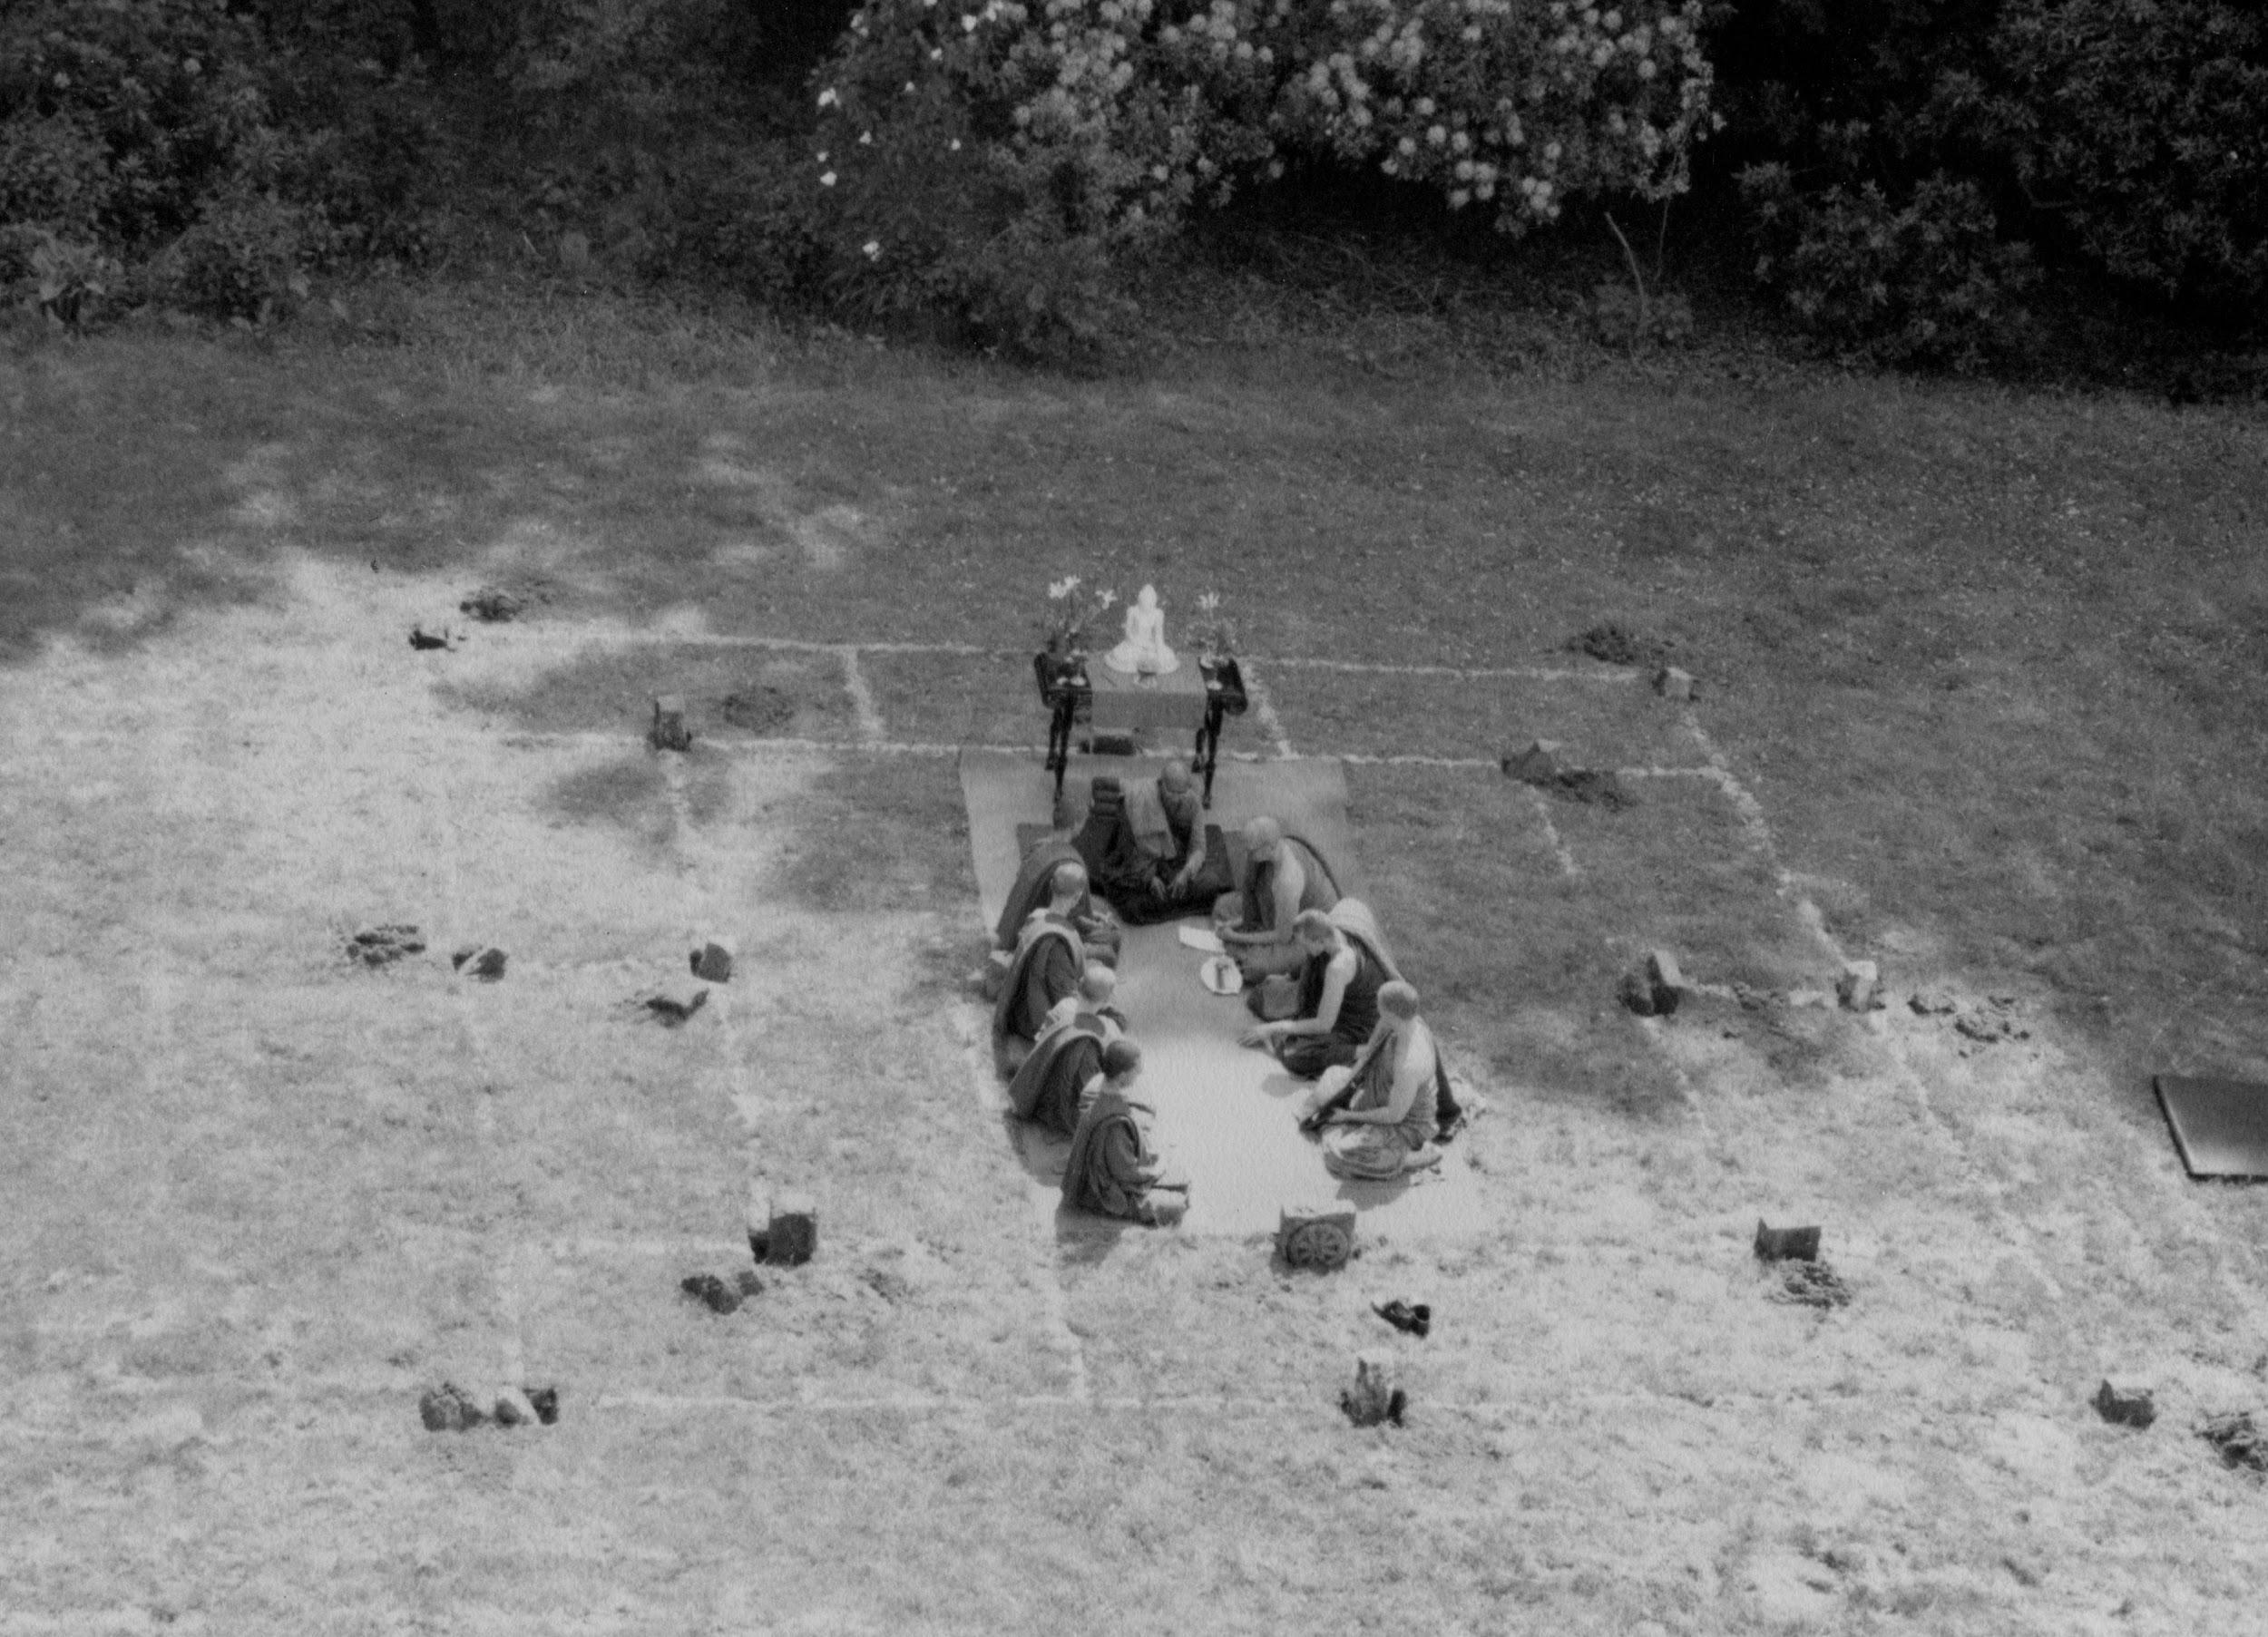
\includegraphics[width=\linewidth]{image6.jpeg}

When it came to the community feeling ready to establish a boundary\cite{sima}
at Chithurst, we had anticipated it would
require a lot of planning and preparation; we hoped that eventually we
would be able to create one out in the Hammer Wood. For Ven. Ananda
Maitreya, who had probably been involved in setting up many over the
years, there was nothing to it. In no time at all, we were out on the
old croquet lawn next to Chithurst House, going through the traditional
chanting: sorting out the possibility that there could have been an old
\emph{sima} boundary there before (from who knows when), and then
culminating in the formal procedure of declaring a new one. Once this
was properly established, the sangha at Chithurst was rightly prepared
to conduct Precept ceremonies. Indeed, for many years after that, this
was the place where all such ceremonies happened.

Bhante Dhammavara\cite{dhammavara} from Cambodia was another venerable Elder who
stayed with us a number of times in those early years. A good lay friend
of the sangha, who moved to live near the monastery, had spent time
training as a monk under Bhante Dhammavara in India. From him I later
learnt that Bhante became a monk around the age of thirty-three after
World War One had ended. Previously he had served as a district governor
and had a wife and a child. He lived as a monk for many years in India,
and a lot of his time was spent setting up and running a natural health
clinic. The first clinic was built in Northern India. After Partition\cite{partition},
it was deemed more suitable that he move to Delhi where, with
the help of Mrs Rameshwari Nehru\cite{nehru}, the wife of then
Prime Minister, Mr Nehru, he set up another
clinic. During his time staying with us at Chithurst, Bhante instructed
community members in ways of using colour for healing. Often this
involved drinking water that had been stored in coloured glass bottles.
For several years afterwards it was normal to come across coloured glass
bottles perched on windowsills around the monastery. In fact Bhante has
a significant repertoire of various skills that he had developed and
used over the years running those clinics in India.

Bhante Dhammavara was staying with us on the occasion that the
Ven. Maha Ghosananda\cite{ghosananda} came to visit. Also from Cambodia, Ven. Maha
Ghosananda had previously been the Supreme Patriarch in that country and
was renowned for his peace marches. When Ven. Maha Ghosananda passed
away in 2007, he was ninety-three years old. When Bhante Dhammavara
passed away in 1999, he was one hundred and ten.

The thing I remember about a visit by the Venerable Piyadassi Thera was
a comment he made during a talk he offered in which he summarized
practice by saying, `Just practise the Dhamma, leave the rest up to
kamma'. So simple that one might overlook its profundity. We easily make
practice complicated because of a lack of maturity in mindfulness,
restraint and wise reflection. Hearing these reminders from such
well-practised monks was significant.

There were also a number of inspiring female Dhamma teachers who
visited. During my time in Devon, Ajahn Sumedho had invited Dr.~Irmgard
Schloegl to use the gardens at Chithurst for her ordination. A retinue
of elders came over from Japan and performed the ceremony according to
their Rinzai Zen tradition, and Dr.~Irmgard Schloegl took on the name
Myokyo-Ni.

On one evening I recall seeing Ayya Khema\cite{khema}
at puja sitting in the midst of our Siladhara community. I
think our paths might have crossed some years earlier in Bangkok when
she was still Ilsa Liedermann. I do recall meeting her husband from back
then, Gert Liedermann, who spent time with us at Wat Pah Nanachat. He
was responsible for introducing the community to foot massage. Ilsa and
Gert had a property near Obi Obi in Queensland, Australia, where they
hosted Ajahn Khantipalo. Later on that property was sold and another
property in New South Wales was purchased, eventually to be known as Wat
Buddha Dhamma, where these days Ajahn Tiradhammo is living. Ayya Khema
went on to request Bhikshuni Precepts within the Mahayana tradition and
settled back in Germany, where she had been born, establishing a centre
called Buddha Haus\cite{buddha-haus}.

Ruth Dennison\cite{dennison}
also visited Chithurst in the early days. She was
one of the formally appointed teachers within the U Ba Khin meditation
tradition. As I recall, she stayed only briefly, but I was pleased some
years later to have a chance to visit her place, Dhamma Dena Vipassana
Center, out in the desert near Joshua Tree National Monument\cite{joshua}.

While reflecting on visits from venerable elders, I also want to
fast-forward a few years and mention the visit in 1990 from Master Hsuan
Hua. He brought with him a large group of his monks and nuns from
The City of Ten Thousand Buddhas\cite{ten-thousand}
in California. The venerable Master must have already
been very advanced in years, but his vitality was impressive, also his
generosity. His style of responding to questions was still very direct.
When one of our young monks who, at the time, was struggling in his
practice, asked a question hoping for some encouragement, Master Hua
told him that practice was like a tiger and it would eat you up. On
another occasion, when some of his monks and nuns asked if they could
learn our \emph{paritta} style of chanting, he scolded them saying they
were only interested in it because of the appealing tune, not because of
the Dharma content.


\chapter{Creative Vigilance}

As a gift on my birthday, I think in 1987, Ajahn Anando generously
arranged for me to be able to visit family and friends in New Zealand.
At the time I was presented with the card, which had the gift inside it,
I was somewhat confused, and maybe wasn't even sure it was for real. I
had not seen that coming. Ajahn Anando was very thoughtful like that.
Exceptional generosity on the part of many lay friends and supporters of
the sangha over the years meant that that was just the first of several
trips back to New Zealand. The same generosity by supporters extended to
financial gifts being given to my parents, since some of the supporters
knew that as monks we aren't able to make such gestures.

It might have been on that first trip back that I met up with an ex-monk
friend, Mark Overton. Some years earlier, after finishing his medical
training, Mark had heard Ajahn Sumedho speak during one of his visits to
New Zealand. This inspired him to travel to Thailand where, eventually,
he took up the monks' Precepts and trained under Ajahn Pasanno at Wat
Pah Nanachat. He then went on to spend a brief period of time training
at Amaravati, before disrobing and once again practising medicine. I
think it was on that trip that Mark and I went hiking together (called
`tramping' in New Zealand) in the stunningly beautiful North West Nelson
Forest Park. On another one of those occasions when he and I were hiking
in New Zealand, I recall how we had climbed a peak in the Southern Alps,
I think it was Mt Sefton; I took a refreshing dip in a glacial lake at
the summit before we walked back down again, and, on the same day, drove
out to one of the many lovely beaches on the coast of the South Island.
I knew the South Island of New Zealand was beautiful, but now I was
seeing it from a different perspective. At one point, as my eyes scanned
the forest that stretched all the way to the mountains in the distance,
I registered how refreshing it was to simply gaze upon the
un-interfered-with. Thank you, Mark, and, again, thank you, New Zealand.

The following year I once more found myself in New Zealand, this time
for a stay of about two months, most of which was to be spent at the
Vihara in Auckland, on Harris Road. Part of my plan was to try and spend
more time with my parents, who had moved to a retirement village near
Orewa, just a few miles north of Auckland.

Early on during this period in New Zealand, I also took the opportunity
to visit with my good friend Jutta in Palmerston North. It was
noticeable on that visit that something had changed for her. Up until
then, I don't remember her ever having shared much about the terrible
suffering she had endured in Dresden, and throughout the Second World
War, but now she spoke more freely. She also shared with me how she had
learnt a particular breathing technique which meant she no longer felt
burdened by so much old pain.

It was inspiring to meet my friend in this new way and I was happy for
her. Whatever spiritual techniques she had learned, or retreats she had
been on, or psychotherapy she had undertaken -- and there had been a lot
-- nothing had led to the integration she was seeking. This breathing
technique seemed to be the medicine she needed. The technique that she
was now working with appeared to be a gentler form of holotropic
breathing as used by the Czech psychiatrist, Stanislav Grof\cite{grof}.
Jutta had earlier tried the Grof approach and found it
too invasive. Later, I believe, she spoke with me about how people
sometimes use this, and similar breathing techniques such as rebirthing,
in a goal-oriented way, and that she was not at all keen on that
approach. Her way was not necessarily looking to relive the birth
experience, or uncover past lives, it was much more here-and-now and, as
far as I could see, more in harmony with dhamma practice. After hearing
about the benefit she derived from this exercise, I was keen to try it
out for myself and she kindly offered to teach me.

The subjective experience that this form of disciplined breathing
precipitated in me defies description or explanation. Suffice it to say
that this technique, which here I will refer to as `connected
breathing', along with a here-and-now, whole body-mind quality of
awareness, brought an end to the fourteen year long `holding pattern'
that I mentioned earlier began after my first vassa.

There are `how-to' books that have been written on this subject, but I
would very strongly advise against trying it out alone. An enormous
amount of energy can be accessed and flood the body in exquisitely
agreeable ways, but that same energy can put you in touch with pockets
of old pain that you didn't know you had. The technique is designed to
put you in touch with such pain, but if at the point of opening up to
it, you re-enact the resistance which caused the pain to become stuck in
the first place, you risk re-traumatising yourself and, in the process,
making your state of imbalance even worse. On the level of mind, we
might like to think we can handle it; the same as when we are on retreat
cultivating metta towards all beings, we might like to think that from
now on we are going to always behave in a kind and caring manner towards
absolutely everyone. But when we actually meet some of those beings,
maybe we find our emotional reactions are not quite so kindly after all.
So long as we are identified with our thinking, we cannot trust our
mind.

This type of breath work can be very effective in putting us in touch
with that which was previously out of reach. Somebody who has worked
extensively with the technique themselves, could recognize, during a
breathing session, signs that point to where and when old pain is ready
to be received yet is still being resisted. Then, hopefully, they will
be able to suggest, at just the right time, in the just right manner, a
change in approach, or perhaps a change in the rhythm of breathing,
which will lead to a deep letting go of that resistance. Once such
resistance is let go of, we will have a much clearer sense of what our
teachers mean when they tell us to be practising `in the body'. Also, we
see more clearly the disastrous consequences of having betrayed
ourselves in the first place by abandoning our bodily intelligence and
taking refuge in thinking. I am not saying that everybody betrays
themselves and becomes lost in their heads, but those who do, suffer a
great deal because of it. In earlier times, the degree of dysfunction
that many of us are defined by these days would have been seen as a form
of madness. If we do find freedom from the madness of being disembodied,
there will be much gratitude.

Back in Auckland at the Vihara, I was feeling grateful for the support
of the Theravada Buddhist community, who had set up a rota of drivers
that took turns in taking me out to see my parents and then bringing me
back again. The same group took it upon themselves to make sure someone
was always there each day to offer a meal. There was a tradition already
established within their community whereby a good number of mostly Sri
Lankans, Burmese, Malaysians and a few Kiwis, would meet for chanting
and meditation each Sunday night. When there was a monk staying at the
Vihara, the numbers swelled. The quality of their interest in Dhamma and
the sincerity of their commitment to meditation and Dhamma practice in
general, was truly impressive. These were not Buddhist-by-name only;
they had a love for the Dhamma and genuinely wanted to make the most of
their good \mbox{fortune} in having an opportunity to practise it. Thinking
about them now, I still find it heart-warming, and I am very grateful to
have met them. In my experience, it is rare to find that quality of
commitment. \emph{Anumodana}.

Other than the visits to see my parents, the daily meal and the
once-a-week pujas, my time was free, which meant I persevered with `the
breathing exercises'. I looked forward to my sessions each day, in the
same way I would look forward to food if I had been starving. It was as
if seeds had been planted a long time ago, but had not had sufficient
water or warmth for them to germinate. Now it felt as if many seeds were
beginning to sprout. A new kind of hope began to emerge. Where I had
felt deeply emotionally and energetically obstructed, I now felt there
was great possibility. I didn't know what those possibilities were, but,
with here-and-now, whole body-mind awareness, that didn't really matter.
This kind of hope was not a naive longing, it was about being positively
oriented towards the future in a way that generated energy, which was
then available to investigate whatever was happening here and now.

Somebody set up a meeting for me one day to see a Christian monk who was
living in Auckland. When we met, he struck me as a dedicated person with
a strong sense of integrity. Some years prior, he had been working (as a
nurse I think) in a hospice in Saigon that was part of the Mother
Theresa's community. During our conversation, he spoke about what he had
witnessed in a number of the Vietnamese patients as they approached
death. He told me that some of those who came into the hospice
professing to be Christians, had previously been Buddhists. He said that
when the end came near, it wasn't to Jesus that they were praying; they
reverted to their faith in Buddhism. What he seemed to be telling me was
that, although these days I called myself a Buddhist, when it came to
the crunch, I could expect to revert to Christianity. What was good
about hearing that was that I didn't feel threatened. Maybe I was
mistaken in what I understood him to be saying, and he was in fact
paying a subtle compliment to Buddhism, but I don't think so. Feeling
that my commitment to Buddha, Dhamma, Sangha was being challenged like
that was helpful. What was about to happen, however, was even more
challenging.

One of the Kiwi fellows who attended the Vihara from time to time, asked
if I would be interested in spending a couple of days hiking along the
coastal footpath just north of Auckland. I jumped at the invitation. We
began at Piha\cite{piha} and walked south. I can't remember now, but I assume he had
arranged for someone to pick us up at the exit point. The description
that follows of what happened during that walk, is an edited extract
from \emph{Alert To The Needs Of The Journey}\cite{alert} Chapter Two (p 15),

\begin{quotation}
We had been hiking for several hours along the coastal footpath; the
weather was hot, and since the beach below us was empty, it seemed fine
to cool off in the water. What I didn't notice was that at the point
where I chose to enter the water, the waves were not breaking. Had I
been better informed about such things, I might have known that the
absence of white-water breakers was a sign that there was probably a
hollow area in the sand beneath the surface of the water, creating a
counter-current that would pull anyone that entered there out to sea;
and being pulled out to sea is exactly what happened to me. My hiking
companion was still standing on the shore, witnessing in desperation the
situation that was unfolding. Many drownings result from just such
situations, when a swimmer is unexpectedly caught in a rip current and
reacts by struggling against it until exhaustion eventually takes over.
Initially, I did struggle, trying to get back to the shore and out of
the danger, doing what I was used to doing whenever I felt threatened:
trying to save myself. But I realized quite quickly that no amount of
fighting to overcome the current was going to work; it was far too
powerful. What did work, thankfully, was surrendering; I flipped over
onto my back and floated: no more fighting, but simply allowing the
current to carry me.

I spontaneously remembered the connected breathing; instead of
struggling, there was deep trusting and a whole-body sense of
surrendering habitual controlling. I found myself drifting out to sea,
floating and breathing. My head was filled with powerful conflicting
thoughts and images: of being eaten by sharks somewhere between Piha and
Sydney; of my parents being upset on hearing that their son had drowned;
of Ajahn Sumedho being annoyed with me for my heedlessness. But at one
point, associated with the effort to keep floating, trusting and
breathing, came the powerful thought, `Let the Buddha take over': my
translation of \emph{Buddhaṃ saranaṃ gacchami} -- `I go for refuge to
the Buddha'. It felt like a battle was going on within me, between, on
the one hand, strong inclinations towards trying to save myself, and on
the other, an impulse towards trusting. The thought that I mustn't give
up the struggle to save myself was fuelled by guilt and distrust, and
when I engaged it, the rhythm of the breathing became interrupted and my
body began to sink. When there was letting go of the contraction of fear
and trusting again, the body felt supported and I returned to floating.
There was no doubt about the intensity of fear coursing through my body;
I definitely did not know that I was going to be OK. At times it really
did look like I might not be. Thankfully, the intimidation of the
impulse to control was outshone by the impulse to surrender into the
breathing, to trusting, to releasing out of the struggle to save myself.

As it happened, the current did drag me out to sea some distance, but
then carried me down the coast and out of the dangerous area, and
eventually the waves brought me safely ashore. Once I was standing on
the beach again I was elated: not just because I was now safe, but
because I felt I had been given the gift of affirmation of practice. In
a modest but significant way, it felt emblematic of what it meant when
the Buddha conquered \emph{Mara}.
\end{quotation}

Back at the Vihara, during the Sunday night Dhamma talk, I chose to
speak about my joy at receiving such an affirmation. I might have even
included some comments about what the Christian monk had suggested would
happen when it came to the crunch. Unfortunately, not everyone picked up
on my sense of gladness, and instead became upset at the thought of
nearly losing their monk. Later, when I considered what had happened, I
realized that talking about that experience in that context was not at
all clever. In fact, swimming in a place that is renowned for rip
currents, was also not at all clever; it was completely foolish. The
good friends and supporters at the Vihara forgave me quite quickly and
for the remainder of my time in New Zealand there were no more such
escapades.

The impact that the connected breathing was having on me was profound.
It did worry me somewhat, since the energy involved was at times so
dramatic. I didn't want to start talking about it with everyone; it was
too important. Also, in monasteries, such bits of news sometimes lead to
ridicule or to becoming the latest fad. It wasn't that I felt precious
about this technique, I just wanted time to see how it would develop.
Also I suspected I would sound evangelical if I began to speak about it
at that stage. This was the most significant aid for integration that I
had come across. I realized, though, that in its power lay its danger.
Perhaps I would lose perspective and go crazy. So I decided to let two
people that I trusted know about it, and then wait one year to see how
it settled. One person I confided in was Ajahn Viradhammo, the Canadian
abbot of Bodhinyanarama Monastery, near Wellington; I either wrote to
him or spoke with him on the phone. The other person was Tan Kittisaro,
and I waited until I was back in the UK before telling him. Obviously both of them
respected my wish for discretion, even if they couldn't directly relate
to my experience.

It might also have been during this period of staying at the Auckland
Vihara that a somewhat rough and ready Kiwi fellow called Blue came to
see me. He was already familiar with our tradition, and was hoping I
would accept an invitation to lead a meditation retreat on his property
out on Great Barrier Island. He offered to make all the necessary
arrangements, so I agreed. Great Barrier Island is easily reached by
ferry from Auckland, and when I arrived there, Blue was waiting to pick
me up, on his quad bike. That was different. His house was only half
built but the weather was mild and the group who had gathered for the
retreat were friendly and interested. I suspect that already, by that
stage, Blue was intent on taking up monastic training. Either way, it
wasn't long before he joined the sangha at Bodhinyanarama and was given
the name Kusalo Bhikkhu. From 2012 until now, Ajahn Kusalo has been the
abbot of Bodhinyanarama Monastery.

When it came time to depart New Zealand and return to Britain, it was
with even more inspiration and gratitude than before: inspiration born
out of association with the fine group of supporters at the Auckland
Vihara, and gratitude for this new skill to which I had been introduced.
Besides the hope I mentioned above, there was a new quality of
confidence, and an increased ability to trust and to feel without being
quite so defended, also a readiness to aspire. All of those qualities
contributed to what these days I like to think of as a state of creative
vigilance: creative, inasmuch as it is agile and interested in
investigating conditions from different perspectives -- not a fixed
position or approach --and vigilant in the sense that it is a state of
aliveness, alertness, and somewhat more ready to meet what life gives
us. Perhaps in Pali it is akin to \emph{saddha}.


\chapter{Our Spiritual Toolkit}

Arriving back at Chithurst I felt renewed and revitalised. From now on,
my practice was more about working with a quality of feeling awareness,
in touch with the body, a much broader perspective than viewing life
from my head. (Of course I hadn't previously been aware of the degree to
which I was identified with my thinking mind). It no longer mattered
quite so much what the sensations were -- gladness, sadness, joy or
sorrow -- the task was how to receive them, how to allow them. Gradually
my ideas about what awakening meant were changing; now I was more
interested in `unobstructed receptivity of everything', or `unobstructed
relationship with everything'. The idea of striving towards some
imagined experience in the future really made little sense to me. This
didn't mean I abandoned all notions of a goal; it meant my relationship
with those notions was changing.

It felt as if up until that point in time I had been listening to music
with the bass turned down. Now the bass was turned way up! Aliveness.
Instead of trying to be free from painful feelings such as anticipation,
for instance, I was now interested in how to feel whatever feeling I was
feeling, without adding or taking anything away from it: learning what
it meant to be \emph{free to} feel that which I was feeling, rather than
struggling to be \emph{free} \emph{from} certain feelings. The feeling
of anticipation, for example, is just a feeling; but there is a space in which that
feeling is arising and ceasing. The feeling is not ultimate; there is
also awareness of the feeling. Now I felt like I had a powerful new tool
in my spiritual toolkit: embodied awareness.

This new tool didn't suddenly absolve me of the pain of guilt and
self-doubt, however. There were still periods when I struggled with a
sense that I was about to be overwhelmed by pain. Sometimes I would have
to tell myself, `Just because I feel bad, does not mean I am bad'. The
bullies of guilt and self-doubt, along with many other apparent
obstructions, didn't disappear, but there now seemed to be a chance that
we could get to know each other.

As a craftsperson will have a variety of tools in their toolkit, so
those committed to awakening require a variety of techniques and skills
to deal with the many challenges he or she is going to encounter on
their quest. Since everyone is different in temperament and talent, we
need to equip ourselves according to our own conditioning. In my case,
it became very apparent that I had been seriously out of touch with my
body, so I needed skills that addressed that particular imbalance. The
breathing discipline I learnt that year in New Zealand helped.

So, too, did frequent visits to see a Vietnamese acupuncturist in
London, called Thong. That he was a Buddhist monk within the Mahayana
tradition and a Tai Chi teacher were also significant. For a period
during the Vietnam war he had been imprisoned, as a monk. After having
been released from prison he disrobed, and, before leaving Vietnam to
come to Britain, married and had a family. Once his family had grown up,
he again requested the monks' Precepts. By that time Thong already had
an acupuncture clinic established in London and was well-known as a
skilled Tai Chi teacher. After many years, I continue to practise the
Qigong form that he taught me. And I believe I continue to benefit from
the many sessions of acupuncture and the traditional Chinese herbal
remedies that he kindly offered me.

Whatever understanding of the Buddha's teachings we might have, if our
body is not in harmony, then life will be a struggle. Maybe some of
those struggles are kammic and unavoidable, but perhaps some of them are
not necessary.

In Theravada Buddhism it is taught that there are three types of
illness: one from which you will recover whether or not you take any
remedy; another from which you will recover if you take an appropriate
remedy, and from which you won't recover if you don't take the remedy;
and the third, where whether you take any remedy or not makes no
difference, since the illness is a result of kamma.
(For a more literally accurate interpretation of what the Buddha said, see
Bhikkhu Bodhi's translation of the Anguttara Nikaya -- `\emph{The Numerical
  Discourses}', Somerville, Wisdom \mbox{Publications}, MA, USA, 2012, Book of Threes,
`Patients', page 217).
Thank you, Thong,
for those treatments, and remedies; for teaching me the Qigong form;
also for your strength and gentleness.

Somewhere I heard or read that, within certain schools of the Tibetan
Buddhist tradition, they won't even introduce you to meditation practice
until you have completed one hundred thousand prostrations. It makes
sense to me now why, in Zen Buddhism, so much attention is paid to the
sitting posture during meditation; if you begin to droop it could result
in your receiving a wack. When Tan Ajahn Chah returned from a visit to
America, he spoke enthusiastically about stories he had heard of the
Chinese Patriarch monk Venerable Bodhidharma. Tan Ajahn Chah was
impressed by how, if Ven. Bodhidharma asked you a question and you
answered it wrongly, you received a whack; if you answered it correctly,
you received a whack; if you didn't answer it at all, you received a
whack. `As for us Theravadins', Tan Ajahn Chah said, `we just carry on
talking about Dhamma, saying it is like this and it's like that, and so
on.' Tan Ajahn Chah also wanted us to get out of the head and come back
into the body.

At one point, I think it was in 1989, Ajahn Sumedho received word that
Tan Ajahn Chah appeared to be dying, and so he quickly departed for
Thailand. As it turned out, it wasn't until January 1992 that Tan Ajahn
Chah eventually passed away. Just before leaving us on that occasion,
however, Ajahn Sumedho had turned to me and, almost as a passing
comment, said that he wanted me to be his substitute at a one-day
seminar due to take place at the Buddhist Society in Eccleston Square,
London. The theme for the day was, `Several Schools, One Way'. By then I
should have been used to how Ajahn Sumedho would occasionally throw a
googly, not just to me, but to anyone in the community. I have never
figured out whether he did that sort of thing as a strategy to test our
agility, or if perhaps he wasn't even aware that he was doing it.
Personally, I wouldn't have expected a relatively inexperienced monk
like me to be standing in for someone of Ajahn Sumedho's stature on such
a public platform -- at least not without some sort of a discussion. An
august line-up of very senior teachers had been planned, including Ven.
Myokyo-Ni representing the Zen tradition, a famous Rimpoche for the
Tibetans, and a well known elder from the Pure Land School. This was an
invitation that did intimidate~me.

On the day of the seminar, I discovered that Ven. Myokyo-Ni was to speak
first and then I was to follow. Ven. Myokyo-Ni gave an inspiring talk,
as always, but all I can recall now was that it was on the Four Noble
Truths. From other conversations I have had with her, I know she never
wanted to be described as a Zen practitioner -- rather she insisted that
she was a Zen Buddhist practitioner. Before being inspired by Christmas
Humphreys and then following Japanese Zen Buddhism, she was already studying
Theravada Buddhist teachings, and always maintained that having a good
grounding in the original teachings was essential. That was all well and
good, of course, but on the occasion of that Several Schools, One Way
seminar, what was there left for me to talk about. One of the things I can still remember about my contribution on the day, was that when they pinned
a microphone onto my robe at chest level, I imagined it was going to
amplify the sound of my heart pounding.

During an interval between the talks, Ven. Myokyo-Ni and I went outside for
a walk by the Square. I took the opportunity to ask for her thoughts on
the situation in which we found ourselves: practising traditional forms
of Buddhism in the West, in an environment that was not always welcoming
or supportive. She turned and focused her gaze on me
and said, `Venerable, when you are doing the real practice, it can
feel like too much, too soon!' Thank you again, Ven. Myokyo-Ni.

On another occasion when Ajahn Sumedho asked me to accompany him to the
Buddhist Society, (not just to deputize for him), his talk had to be
interrupted because there was a distracting amount of smoke rising up
from behind where he was seated. As usual, he was sitting on a zafu in
front of the shrine in the main meeting room of the Society. There was
no mistaking it being smoke, and it wasn't a small amount which could
have come from the sticks of incense. What had happened, it seemed, was
that when he had lit the candles and incense as a preliminary to the
occasion, a spark must have dropped onto his zafu, igniting it. Somebody
helpfully removed the smoking zafu and the talk continued.
Interestingly, quite a long time afterwards, when we went to leave the
Society buildings, we found a bright glowing orb sitting on the pavement
outside the front door. That helped me appreciate why kapok filled
zafus, although preferable to sitting on a polyester-filled one, are
considered a fire hazard; once they start burning it is difficult to put
them out.


\chapter{Ordeal in the Attic}

In part because of the confidence that had arisen from being more in
touch with my body, and because of the sense of hope that the breathing
exercise had given me, when we were preparing for the 1990 Winter
Retreat at Chithurst, I asked Ajahn Anando if I could determine to spend
the two months in solitude. I was interested to see what the increased
intensity would bring up. There were other motivations as well, but
having a chance to meet myself in solitude was appealing. It turned out
that I overreached with that determination.

The room I was living in was in the attic, and the floor space was
roughly three by four metres (there were also two sizable raised
platforms). I covered the windows with tracing paper so light could come
in but I couldn't see out. The idea behind that was to intentionally
frustrate any impulses to distract myself from what was going on inside
of me. Somebody left food outside my door each day, and during the
community's morning chanting period, I would take my slop bucket down
and empty it in the bathroom. Other than that, the only time I left the
room in those two months was to participate in the fortnightly
recitation of the Rule.

Very soon after the retreat began, I was assailed by intense anxiety.
Much of the following two months was spent doing whatever it took to
survive the onslaught of fear and dread. I find it impossible to compare
the horror I endured during those two months with what had occurred at
Wat Hin Maak Peng in my first Rains Retreat, since somehow I was not the
same person. I had accumulated many experiences over the approximately
sixteen years since then, and acquired new skills. None of those skills,
however, protected me from having to go through what turned out to be
another agonizing ordeal.

At one point during the retreat a severe storm struck and, as a result
of my confusion, I was consumed by feelings of fear that I personally
had caused the storm. On this occasion I broke my silence to enquire
whether anyone had been killed in the storm. To say I was consumed, is
partly an exaggeration, since if I had truly been consumed I would not
have survived. I did survive, but the intensity was way more than I
bargained~for.

After the Winter Retreat ended and I again joined the community for
evening puja, Ajahn Anando invited me to give a talk. My memory of that
occasion now is that the act of opening my mouth to speak required such
a huge amount of effort -- so much intensity had built up over the two
months -- that I spoke only one sentence.

It took some time before I could find a sense of balance again. My
confidence hadn't been shattered -- not at all -- but it now had a
companion called modesty. All those hours spent bathing in exquisite
bodily sensations associated with the breathing exercises, hadn't driven
me crazy, but they had led to a degree of delusion. I think the bass had
been turned up a bit too far.


\chapter{The Forest Sangha Calendar}

When we had received word that our teacher, Tan Ajahn Chah, might not be
with us much longer, it occurred to me that we could mark the occasion
with a pictorial calendar -- something that could be printed and
distributed around the world to the increasing number of branch
monasteries and their supporters.

In part, my motivation was to find a beautiful way of honouring the life
of our teacher. Also, in equal part, it was to produce something that
would offer the extended community of lay disciples of Tan Ajahn Chah a
sense of belonging. We all benefit from feeling like we belong
somewhere, and if that somewhere is a spiritual community for which we
have respect, then all the better. It seemed to me that having a
calendar hung on the wall throughout the entire year, one that you could
look at regularly and be reminded of the community of which you were a
part, would be beneficial. A young fellow called Pete, who was
frequenting Chithurst in those days and was a graphic designer, kindly
offered to assist me in compiling such a calendar.

This was the beginning of the annual Forest Sangha calendar\cite{calendar}
that has been produced each year, except one,
since 1990. The design has altered somewhat over the years, and the
production and distribution has changed, but as far as I can tell, the
function has remained much the same. It has been a privilege and a
pleasure to have been involved in this project all these years. I say
`involved', because it depends on many more people besides myself to
produce it. The final selection of photos and quotes has been my
contribution, but I have had the assistance of a good number of others
when it comes to design, layout, printing and distribution. The process
of acquiring the astronomical (and astrological) dates for many years
depended on when the royal palace in Thailand would release them. These
days, thanks to an algorithm skilfully generated by Tan Gambhiro and
colleagues, we are able to calculate the dates with excellent accuracy,
without having to wait to hear from others. Initially the calendars were
printed in this country and shipped abroad. For many years now, thanks
to the generosity of the Kataññuta Group in Malaysia, they have been
printed and distributed from there.

Not everyone in our sangha agrees with my personal preference
(influenced by Marshall McLuhan's \emph{The Medium is the Message}) for
black and white images, and my view that they more effectively
communicate the message, `less is more'. The world is intoxicated, in my
opinion, with excess sensory stimuli. The idea of producing a
full-colour calendar could be tempting in the same way that over-eating
of cakes and cookies could be tempting. Our message, as far as I am
concerned, is: if we are seeking clarity and contentment, either as a
samana or as a householder, then simplification is what is called for --
not proliferation. This is one of the central themes in the teachings of Tan Ajahn Chah,
as I understand them. It is not merely a matter of aesthetics (although
I acknowledge that is a factor).

Then there have been a variety of opinions about the sort of photos to
publish. The first year consisted exclusively of images of Tan Ajahn
Chah. If we had continued doing that, it could have fed into the notion
some people had that we were a sort of cult. For a while it seemed that
nice pictures of nature would be a good way of representing the Forest
Sangha. One year we used images of shrines in the various branch
monasteries. On occasion I would receive an objection because somebody
didn't think a photo I had selected looked quite right. Then there have
been requests that we have more photos of monks' and nuns' faces; at
other times, requests that there be less photos of faces. For many years
now the photos have simply been of people doing things in monasteries.
Since we regularly receive messages of appreciation and there are 18,000
copies printed annually, it must still be serving a useful
purpose.

Selecting suitable photos for these calendars is always fun; however, an
equally rewarding part of the project is finding the `just right' Dhamma
quote: one that resonates with the image. In the early years we used
extracts from translated teachings of Tan Ajahn Chah. More recently we
have been alternating, year by year, Tan Ajahn Chah's teachings with
verses from the Dhammapada. When our efforts are successful, the image
generates an atmosphere that makes users of the calendar susceptible to
the message contained within the Dhamma quote.

Towards the end of 1990, I was told that I would be moving to
Northumberland to take over leadership of the community at Harnham. With
the development of more branch monasteries in Britain, Switzerland,
Italy and New Zealand, a pattern was beginning to emerge whereby abbots
would be moved on roughly every two years. The idea behind that was to
try and avoid anyone becoming overly attached to one place. This wasn't
the only reason Ajahn Sumedho sent me to take over at Harnham in
Northumberland, but it fitted in with the pattern. A second monk was to
join me, Tan Vipassi. Before heading north, he and I spent the Winter
Retreat together at Amaravati.


\chapter{Heading North}

The winter retreat that year lasted for the two months of January and
February. This was the first time I had lived at Amaravati. I was
invited to stay in a room often used by visiting senior sangha members,
which meant that although the weather outside was cold and miserable, I
was warm and comfortable, for which I was very grateful.

Although the accommodation and routine were agreeable, my mind was
preoccupied with what I imagined might lie ahead at Harnham. Amaravati
and Chithurst were sister monasteries in more ways than one. Regular
exchanges of residents took place between the two communities, and they
were both run by the English Sangha Trust. The monastery at Harnham was
managed by a completely separate and independent body, these days called
Harnham Buddhist Monastery Trust\cite{harnham-trust}.

I had visited Harnham monastery before, and I confess I found the
buildings and the surrounding countryside somewhat bleak. That might
have been because my visits coincided with the Kathina season which
always falls in autumn. Whatever the reasons for my reservations, that
retreat period gave me plenty of time to look and feel into where, when
and how I was creating suffering out of something that I was only
imagining. Perhaps it would all be wonderful, with a community of monks,
novices and anagarikas living in a cooperative manner, with attentive
trustees supporting the sangha -- all in an effort to create something
profoundly beautiful. Of course, I didn't know.

Thankfully, part way through that retreat, I came to realize that many
of my worries were a result of the way I held the idea of leadership. I
have written in \emph{Servant of Reality}\cite{servant}, (p2) about how, one morning,
while reflecting on the words of our morning chanting, \emph{I am a
servant of the Buddha, I am a servant of the Dhamma, I am a servant of
the Sangha,} a fresh perspective on the idea of leadership opened up.

A wonderful feeling of relief came over me as I recognized how appealing
I found the suggestion of being a servant. And how different holding
that image in my mind felt, compared to the idea of being a master. It
was obvious that I really didn't want to be a master. I began to see the
extent to which I had been struggling to try and master everything:
trying to master my meditation, master my relationships, master my
understanding of Dhamma. It was just deluded personality yet again,
trying to control everything. I started to realize that not only did I
not want to be a master, but nobody had ever told me that I had to be
one. I could be a servant if I wished. With this recognition, a burden
fell away. The unconscious commitment to compulsively controlling was
seen just a little bit more clearly. My vision of Harnham, and whatever
the future might hold, was transformed.

Being a leader of a community is a way of serving that community; it is
not merely a way of controlling it. This change in perspective helpfully
influenced how I would navigate the vicissitudes of community life over
the following years.

There never had been any good reason for concern about what I would find
when I arrived at Harnham. Amongst the six or so residents living there
at the time was one with whom I was already somewhat acquainted. Tan
Suriyo I had known as Robin when he was an anagarika at Chithurst and
was my driver and chaperone on a number of occasions. He took monks'
Precepts at the same time as Tan Puñño, and I had the good fortune of
being their mentor during the period of transition from anagarika to
monk. There was also a particularly helpful anagarika from Boston,
called Chris (these days known as Ajahn Jayanto). Tan Suriyo and he were
from a similar part of America, and they each contributed to an
atmosphere of goodness and integrity. Sometimes I imagine that in the
future scientists will develop a way of measuring an individual's
integrity, similar to how these days they measure intelligence. Maybe in
the future IQ will stand for Integrity Quotient. I estimate these two
men would score very highly.

Another unexpected and agreeable aspect of the move was finding that
there was a Dhamma Hall building project well underway. The nitty-gritty
work of excavation and outer construction was virtually all complete,
and the building was now ready for the next, thoroughly pleasing, phase
of interior design. It could hardly have been a more welcome task. Of
course it wasn't without its challenges. The first decision to be taken
was regarding a large bay window that had been planned to sit behind the
main shrine. From what I had learned in consultations at Chithurst,
according to the Chinese concept of \emph{feng shui}, there should never
be a window behind a Buddha image. I cannot substantiate that in any
way; however, the sense I have of how it would feel to be looking at a
Buddha image with trees and possibly even people moving in the
background, is not one of stillness. When I look at a shrine I want to
feel stilled. So I took the decision to cancel the bay window project
and had the construction workers continue building the wall all the way
up, but leaving an opening on top for an atrium, so light would descend
down from above the Buddha. The decision wasn't met with the approval of
everybody but I was unwavering. Nearly thirty years later, and I am
still convinced it was the right decision. We don't go into a spiritual
sanctuary in order to gaze outside at the view.

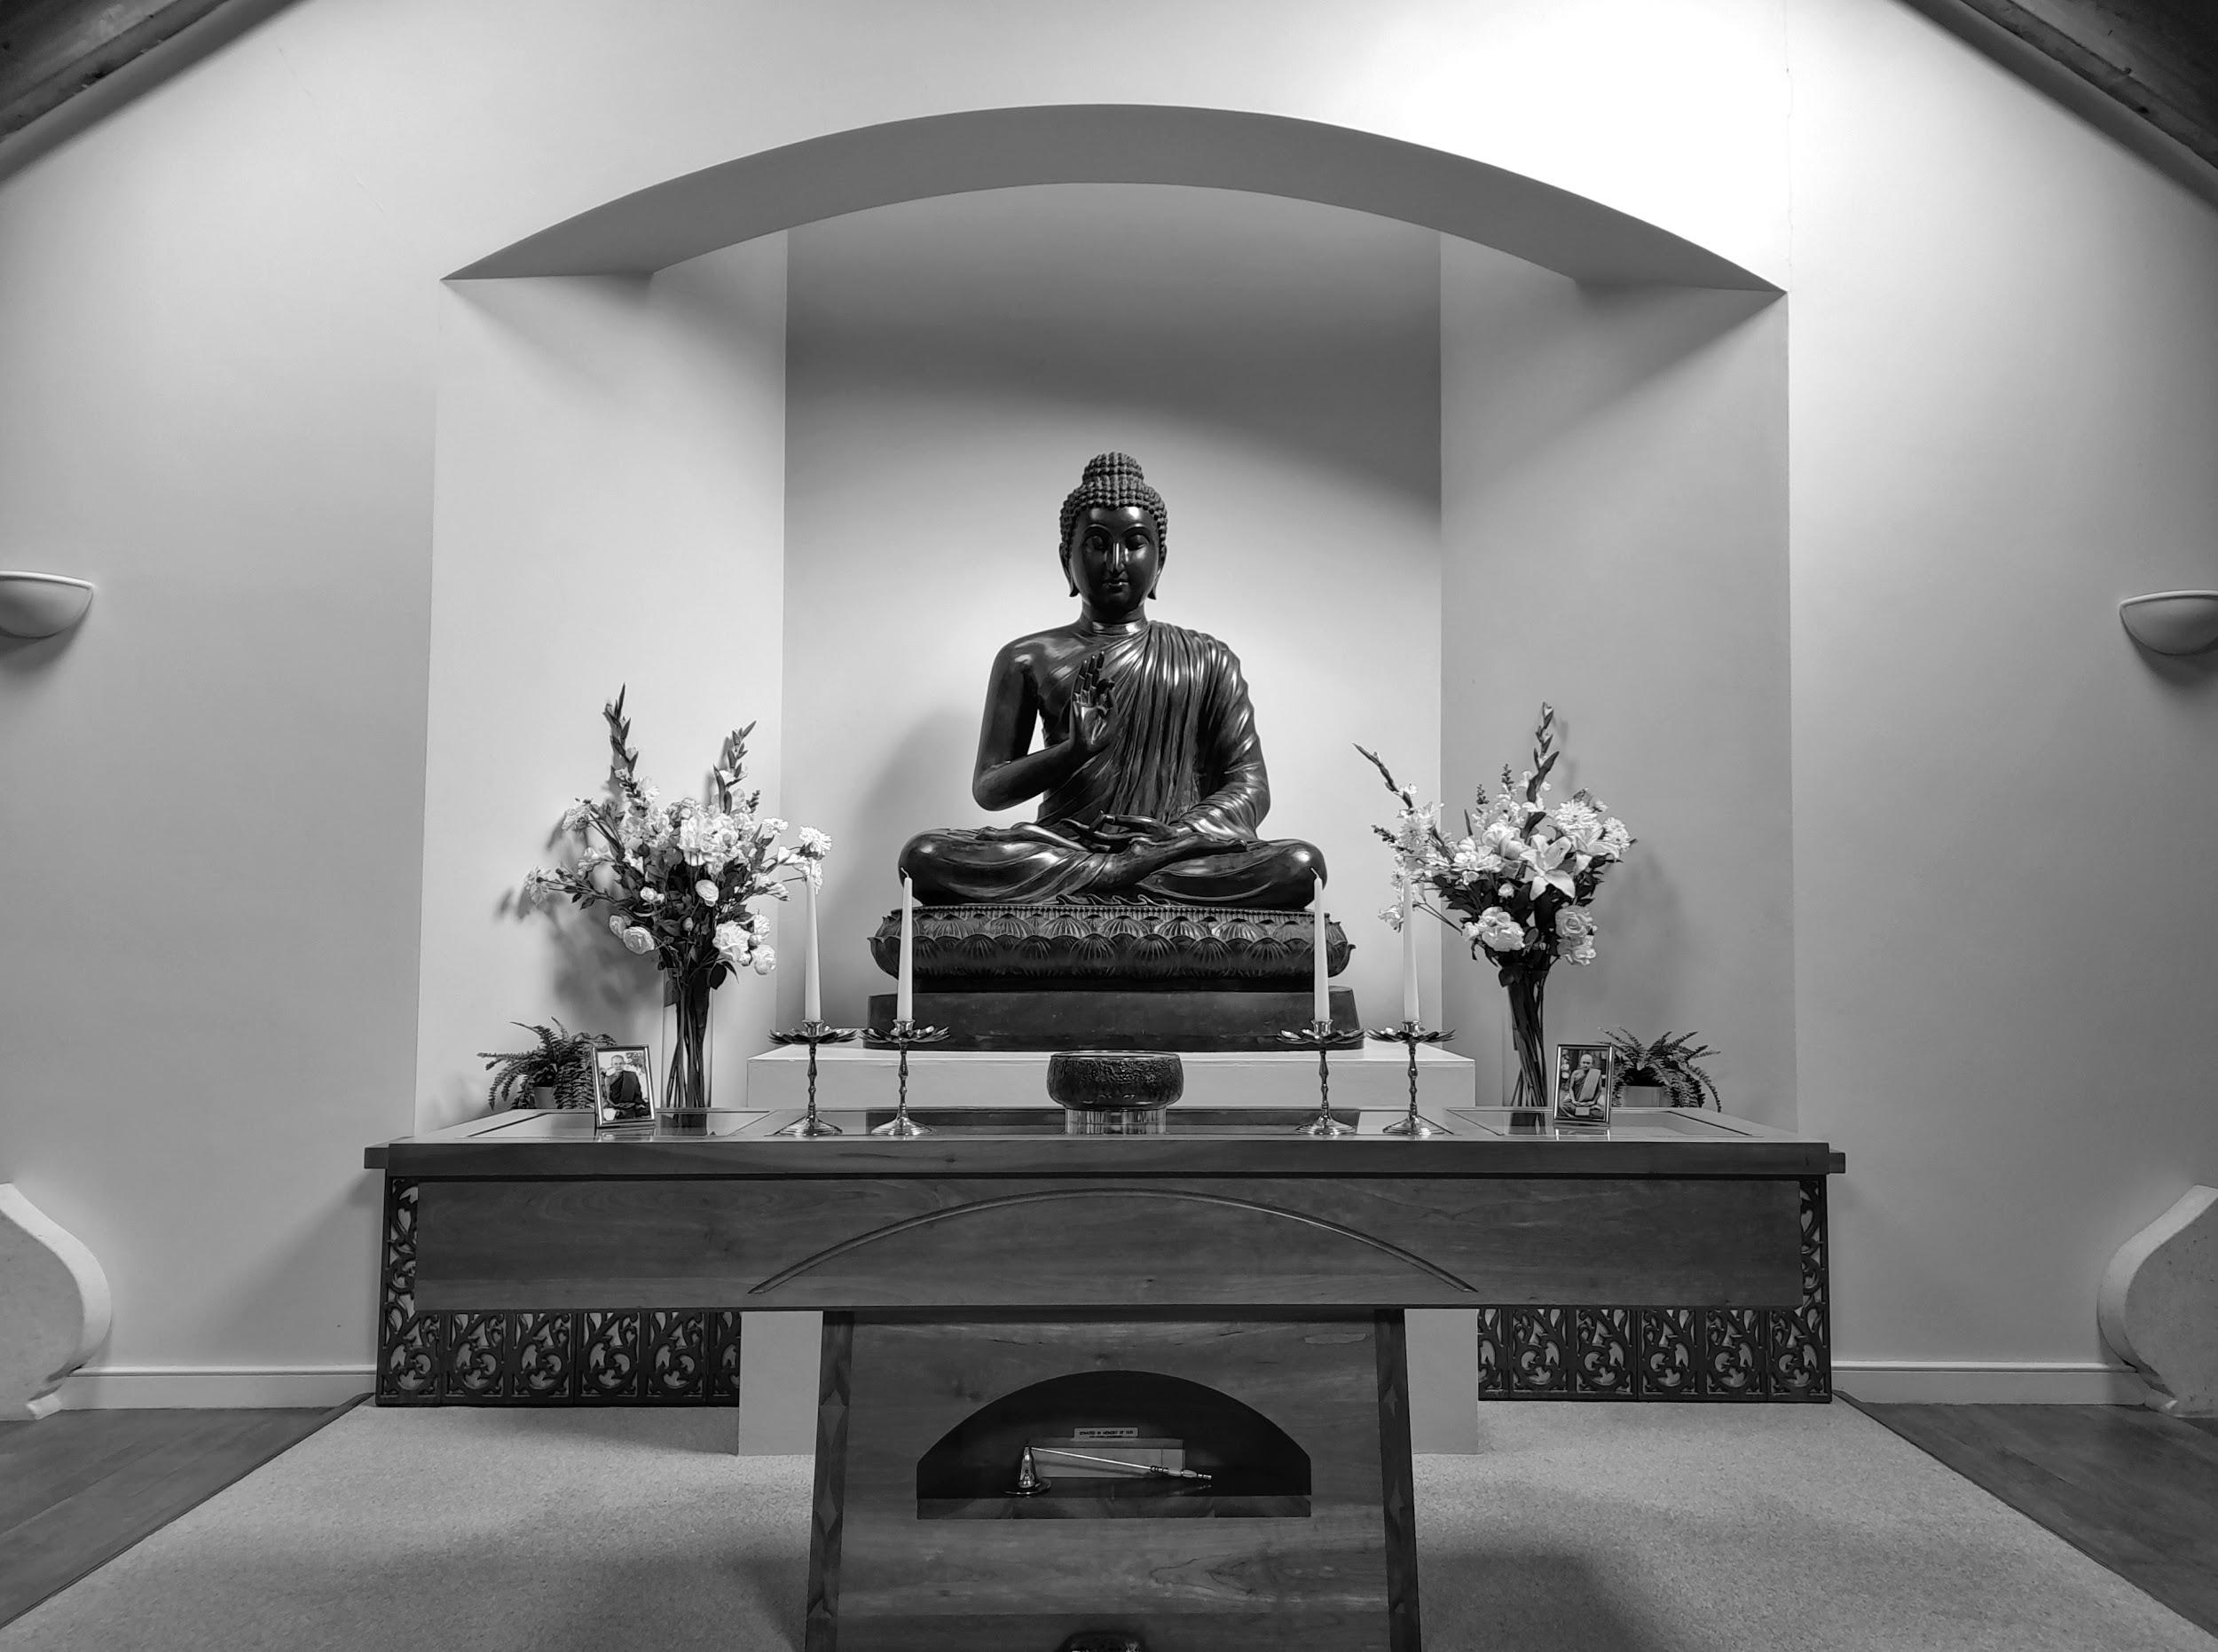
\includegraphics[width=\linewidth]{image7.jpeg}

Tan Vipassi and I considered very carefully how we should approach the
period of my taking over as leader. The previous abbot, Ajahn Pabakharo,
as mentioned earlier, had been a helicopter pilot during the war in
Vietnam. He was a tall and imposing figure. He spoke with a commanding
sense of what was needed, and seemed to relish any opportunity to use a
chainsaw. He and I could hardly have been more different.
Understandably, it was going to take time for the resident sangha to get
used to the style of this new leaner, quieter Kiwi abbot; also, the
trustees would have to get used to yet another way of doing things. I
was the fifth senior incumbent in the ten years the monastery had been
running. Tan Vipassi and I decided that we wouldn't change anything that
wasn't necessary for the first six months: just observe and wait until
we had a good enough overall impression of the place and its people.
That decision worked well. As the weeks and months went by, a new
configuration of community dynamics was emerging, building work
proceeded without too many hiccups, and everyone seemed to be
cooperating well.

The month of May in that first year marked approximately ten years since
Harnham Monastery had begun, and it felt fitting to have some sort of
celebration. The occasion was modest but rewarding and I am pleased we
did it. I was also pleased that the ceremony we organized later that
year in September to celebrate establishing a \emph{sima} boundary
inside the new Dhamma Hall went so well.

Senior sangha members from various monasteries down south were invited.
Eight handsome bodhi leaf-shaped `\emph{sima} markers' were carved by a
local craftsman, along with eight large and very heavy stone spheres
that were used in the formal designation of the \emph{sima} boundaries.
As at Chithurst, we went through the process of removing any possible
previous \emph{sima} boundary, and then established the new one. It was
conducted with an attitude of dignity and respect as befits such an
occasion.

It was also later in that first year, 1991, that the main
\emph{Buddha-rupa} for the Dhamma Hall arrived. When Ajahn Pabakharo was
still abbot, he had made arrangements for it to be cast in Thailand, and
it was sponsored by a long-time \emph{looksit} (disciple) of Tan Ajahn
Chah's, Khun Siri. On receiving notification that a half-metric-ton
image was due to arrive, no small amount of trepidation was triggered
within me. Over the years I had seen many large Buddha images that were
far from inspiring to look at. The image that was about to arrive would
grace our Dhamma Hall for ever; whatever it was, was what we would be
bowing to from now on. Ideally, of course, one would be making an effort
to maintain equanimity, but \emph{upekkha} is a virtue in which I was,
and still sadly am, undeveloped. I wanted our Dhamma Hall to be a space
in which the Thais, Burmese, Sri Lankans and Westerners, would all feel
uplifted when they entered. If the central Buddha rupa on the shrine
looked garish and out of proportion, that was going to be difficult. I
assume I knew enough about practice back then to appreciate that wanting
was not the problem, it was clinging to wanting which led to suffering,
but I wasn't able to let go. I \emph{really, really} wanted it to be
inspiring, so I suffered accordingly.

On opening the crate, I saw that my concerns were, once again,
groundless. The bronze Buddha image had been superbly crafted and cast;
because of the unpolished finish, it had a slight green patina, the
colour of the moss on the stone walls. Immediately upon seeing it I was
relieved. \emph{Anumodana} Khun Siri and everyone else who was involved
in making this offering. For my part, I continue to work on developing
equanimity.

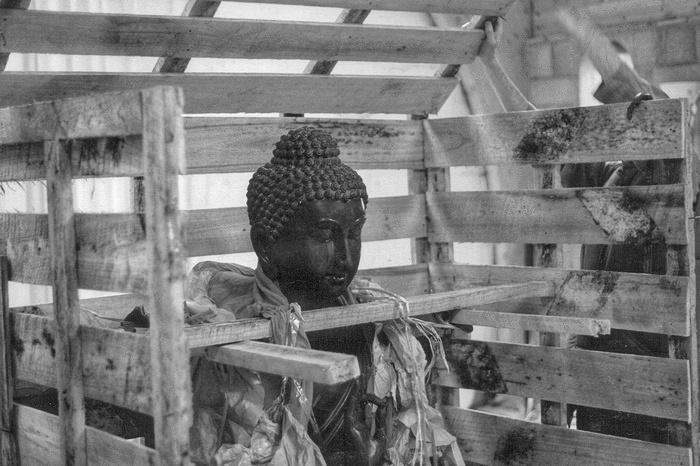
\includegraphics[width=\linewidth]{image8.jpeg}


\chapter{Tan Ajahn Chah's Funeral and Teachings}

On January 16th, 1992, our teacher, Tan Ajahn Chah, passed away. He had
appeared to be near death for several years, so that when the time came
it wasn't a terrible surprise. There was of course, nevertheless, a
sense of loss. Some of the sangha from down south travelled out to
Thailand to participate in the chanting sessions honouring his life and
his teachings. In keeping with Thai custom, occasions such as the
passing of a great Dhamma teacher calls for a very special event. In the
case of Tan Ajahn Chah, there was going to be an extended period in
which many thousands of disciples, monastic and lay, would gather at his
monastery, concluding with His Majesty The King of Thailand coming to
pay his respects before the actual cremation. All that would require a
great deal of preparation, so the date for Tan Ajahn Chah's funeral was
set for the following year, 16th January 1993.

At Harnham we established a week-long routine of evening sitting
meditation and chanting, ending with a public event, during which I read
out one of his translated talks, Not Sure\cite{collected}; a teaching on
uncertainty. A special shrine was set up
in the meditation hall on the Dhamma Seat. Our teacher had gone; we were
now left with the teachings.

One of the great appeals of Tan Ajahn Chah's manner of teaching was the
way he used similes. He was skilled in turning everyday situations into
Dhamma lessons. When he spent time in Britain he visited Edinburgh, but
that was well before the monastery in Northumberland was established.
Had he spent time here on Harnham Hill in these old stone buildings, he
would very likely have had something to say about the conditions to
which we were having to adapt.

There was a very good reason why the roof tiles on many of the buildings
on Harnham Hill were made out of thick stone slabs; the winds that
sometimes buffeted us were forceful. The walls of the stone buildings
were thick, also for a good reason; particularly when the winds blew in
from the north, they could be very bitter. The nearby city of Newcastle
upon Tyne is on approximately the same latitude as Moscow.

However, the winds from the north were not the only challenge we had to
handle. We certainly also had our share of being blown around by the
eight worldly winds: praise and blame, gain and loss, pleasure and pain,
honour and insignificance. In the Mahamangala Sutta\cite{mahamangala}
(p39), in the third to last stanza, the Buddha
describes how the heart of one who has insight into the Four Noble
Truths reacts when impacted by the worldly winds,

\clearpage

\begin{quote}
  Phutthassa loka-dhammehi,\\
  cittam yassa na kampati,\\
  asokam, virajam, khemam,\\
  etam mangalam-uttamam

  `Though subjected to the worldly dhammas,\\
  the heart (of one who has insight into the\\
  Four Noble Truths) will remain unshakeable,\\
  griefless, dustless, secure.\\
  This is the greatest blessing.'
\end{quote}

The land and buildings surrounding Harnham Monastery were owned by Mr
John Wake, or Farmer Wake, as he was known. The main building, which the
sangha occupied, had been in a semi-derelict condition when Farmer Wake
originally let it to us. Eventually, once repairs had been done, he
would often join in with the sangha for the midday meal. From time to
time the monks would help him out with tasks around the hundred-or-so
acres of farmland. He was already in his eighties by then and could use
the help. He seemed to enjoy having the company of the community on the
hill. Often he would talk about the history of the place, including the
period when an earlier owner of the property,
Madam Babington\cite{babington}, had lived in the Hall and was eventually buried in
a crypt not far from the main house. There had also been a small chapel
that she had built near the walled garden. Some say the ghost of Madam
Babington still appears on the hill.

In the early years, Farmer Wake took part in our festival events,
including a circumambulation on Vesakha puja. I~remember on one
occasion, around the time when the building of the Dhamma Hall was newly
completed, he came inside to see the result of all our work, and
commented, `What a pity that your teacher didn't live long enough to see
this'. Thank you, Farmer Wake, for being so broad-minded and big-hearted
as to welcome a bunch of Buddhist monks onto this wonderful Hill.

In those days, we received regular visits from members of the Leeds and
Edinburgh meditation groups. They were generous and energetic in helping
with the ongoing building projects. One of those visitors was a young
student called Timmy, who was studying Russian at Edinburgh University.
His mother was Thai and his father Malaysian; he seemed keen to help out
and fitted in well. These days he is known as Ajahn Siripañño and serves
as leader of the sangha at a remote residence near the border between
Thailand and Myanmar, a place called Dtao Dam, or The Black Turtle
Hermitage.

\enlargethispage{\baselineskip}

In January 1993, nearly all the senior Western sangha disciples of Tan
Ajahn Chah were gathered at Wat Pah Nanachat. The schedule had been
skilfully arranged so that, besides our having time to participate in
the events taking place nearby at Wat Pah Pong, we also had quality time
together, meeting formally and informally. There was at least one large
meeting in the main \emph{sala}, to which everyone was invited -- monks,
novices and nuns, residents and visitors. I was asked to facilitate. The
atmosphere was surprisingly harmonious and the Q\&A session was not
difficult to mediate. I say surprisingly, since having such a large
group, of mainly men, from different backgrounds, and most of us
strong-headed, differences of opinion were inevitable. I would say that
in a large part the concord was a result of the very grounded
approach Tan Ajahn Chah had towards monastic community life in general,
and towards \emph{Vinaya} in particular.

\enlargethispage{\baselineskip}

\emph{Vinaya}, or the monastic code of discipline, in its original form
was an expression of the wisdom and compassion of the Buddha himself.
However, there are a great variety of interpretations of just how to
apply the many rules and procedures included within that code of
discipline. Approximately two thousand six hundred years ago it had been
spoken in a dialect known as \emph{Magadhi} (with some possible other
related dialects) and was recorded in the Pali language within the first
two hundred years after the Buddha passed away. Pali was not a generally
spoken language (the word Pali actually means `text'); some scholars
think it is somewhat similar to esperanto\cite{esperanto}
inasmuch as it was intentionally generated for a specific
purpose, in this case to codify recorded teachings. These days there are
still many scholars who can understand it, and these Pali texts are
available to consult when seeking clarification on particular points.
Tan Ajahn Chah's approach was to show respect for the tradition and for
the theoretical (\emph{pariyatti}) aspect of our monastic training, but
to always remember that the point of these teachings and traditions is
to awaken to the truth that lies beyond our habits of clinging. Hence a
lot of care is required to avoid falling into the trap of seeking
security by clinging to the \emph{Vinaya}. In other words, remember to
keep your feet on the ground.

At the gathering at Wat Pah Nanachat, there were not just the large
group meetings; there were, for example, other meetings that involved
the abbots of formally appointed branch monasteries. These various
meetings, large and small, were the harbinger of the now
well-established tradition of senior sangha members meeting up
approximately every three or four years to discuss shared concerns. It
was the first opportunity we had to see ourselves as this evolving
worldwide community, and to begin to acknowledge how we were going to
have to work to maintain cooperation. As I said, most of us were
strong-headed and had our own views on things; however, again, I think
it was because of Tan Ajahn Chah's example, and the value he placed on
cultivating cooperative community, that we managed to meet in harmony
and express differences without too much difficulty.

One example of an issue that we successfully navigated our way through
to a mutually agreed solution, was to do with traditions around bowing.
In Thailand, tradition dictates that when paying respects to an elder,
first the sangha of bhikkhus bow, and the elder acknowledges them by
holding his hands in \emph{añjali}. This would then be followed by the
novices, nuns and laity all bowing, with the elder having lowered his
hands. There is an explanation within the \emph{Vinaya} for how this
practice might have developed, but we felt that in this case, where
Buddhism was rapidly spreading to many very different cultures, there
was room for another interpretation. We discussed how, outside of
Thailand, it would more likely lead to harmony and mutual benefit if
everybody bowed together. It was encouraging to find that as a group we
were able to listen to each other -- both those of a traditional
persuasion and those keener on adaptation -- consider the variables, and
eventually arrive at an agreement by consensus. As far as I know the
decision taken at that meeting has never caused any disruption.

It is not insignificant that the Buddha established consensus as the
primary principle involved in making formal decisions in the sangha. In
some cases a decision made by majority vote can still stand; however, it
is better to make the effort to reach a consensus. It can take a
considerable amount of time and patience to reach a decision by true
consensus, as it requires that all those involved in making the decision
feel included. It doesn't require that everyone has exactly the same
view -- that would be unanimity. On any matter of substantial
importance, it is likely that not everyone will hold exactly the same
view, but it is possible that people holding a divergence of views can
all agree on a single course of action. I don't know if social
psychologists have ever done studies on this subject, but if they did, I
expect they would find that when a course of action is decided upon by
way of consensus, there is a better chance of everyone respecting that
decision, because they were all involved.

As an aside, I want to deviate briefly and comment on what has been
happening here and now, in July 2020. As mentioned above, that gathering
at Wat Nanachat in January 1993 was the first in a series of such
gatherings. I don't think we had a name for it at the time since the
main purpose for our being there was the funeral of Tan Ajahn Chah. Over
the years, however, a variety of acronyms have been used to describe
these gatherings: WAM for `World Abbots Meeting'; GEM for `Global Elders
Meetings'; IEM for `International Elders Meetings'. Currently, when
referring to the smaller meeting of abbots only, we are using BAM, which
stands for `Branch Abbots Meeting'. The name change factors in the
difference between the formally appointed Branch Monasteries\cite{branches},
of which there are now fifteen, and the more loosely
affiliated Associated Monasteries, of which there are maybe eleven or
twelve. The fifteen abbots who constitute the BAM group are tasked with
discussing and hopefully reaching decisions on matters pertaining to
these monasteries outside of Thailand. (The abbot of Wat Pah Nanachat in
Thailand is also included). As it happens, the stage I am at currently
in writing these reflections, has just coincided with two days of
meetings of these branch abbots. A gathering, probably in Thailand, was
due to take place around now, but the Covid-19 pandemic meant that was
not possible. The meetings of the past two days took place via the
internet and were hence referred to as v-BAMs, `virtual Branch Abbots
Meetings'.

It is noteworthy that, for roughly a third of the participants, this was
their first abbots' meeting; their predecessors, who probably attended
that meeting in January 1993, have all recently relinquished their roles
as abbots. In advance of these meetings I was considering the fact that
there would be a new configuration of participants, but wasn't
especially concerned. Experience over the years has taught me that there
are grounds for trusting in the goodness and competence which results
from right practice. The six hours of these virtual meetings were not a
picnic: they were work. On the practical level alone, accommodating the
different time zones was tricky enough; some participants were up at two
o'clock in the morning. And inevitably, of course, there were issues
with technology: several of us were at school when the very first
computers were being invented, and not all monasteries have a high speed
internet connection. The more challenging aspect, however, was to do
with how we might raise matters of concern with each other, listen,
discuss and agree, or disagree, and at the same time honour our
commitment to harmony. Given the enthusiasm expressed by all
participants for holding more such events, I would say the meetings were
a wonderful success. I continue to marvel at, and feel grateful for, the
skill Tan Ajahn Chah displayed in his way of imparting the training, and
the beauty of the legacy he left behind. What he gave us was a way of
living in spiritual community with an emphasis on the spirit, not merely
on the form; his way was to cultivate a quality of mutual respect which
allowed for individual differences without compromising concord.

Now back to 1993. On the day of the cremation ceremony itself, there
were approximately 500,000 people\cite{cremation}
at Wat Pah Pong, including the Supreme Patriarch, Ven.
Somdet Nyanasamvara of Wat Boworn, and Their Majesties the King and
Queen of Thailand. From what I could tell, the \mbox{overriding} atmosphere
during this phenomenal event was one of reverence and respect, gratitude
and sadness. It is rare that such beings as Tan Ajahn Chah appear in the
world; it is natural that we feel grateful, and understandable that we
feel as if we have lost something precious. When the Buddha was dying
and was asked who would take over leading the sangha once he was gone,
he pointed to the Dhamma, saying that was to be the teacher. I am sure
Tan Ajahn Chah would likewise have pointed to the teachings.

Anyone who has listened to talks that I give\cite{talks}
would probably have noticed how often I refer to
Tan Ajahn Chah. Perhaps, also, they have observed that there are several
teaching stories or situations on which I regularly comment. In this context of reflecting back on the life of Tan Ajahn Chah, there are twelve points which I wish to highlight; seven of these I have written about earlier in these notes, but I will list them all here again.

The first, is a teaching shared with me by a Western monk (earlier referred to
as Tan Cittapalo) who was visiting when I was still living at Wat Boworn in
Bangkok.
On that occasion I asked him what
Tan Ajahn Chah had to say regarding right view. Tan Cittapalo said that
Tan Ajahn Chah teaches that even the Buddha's instructions on right view
become wrong view when we are clinging to them out of unawareness. This
introduced me to the emphasis Tan Ajahn Chah placed on being mindful of
how we hold the teachings and the training, rather than merely
struggling to get the `right' idea and becoming attached to it.

The second teaching I would mention is that of experiencing Tan Ajahn
Chah's warmth and sensitivity at Wat Pah Nanachat when my foot was
seriously infected. Some teachers, it seems, insist on always presenting
the highest Dhamma and, unfortunately, in the process, tend to forget
the benefits of shared human companionship. On that occasion, where I
was suffering physically, Tan Ajahn Chah didn't tell me to tough it out;
he offered me his warm-heartedness.

Then there was a time when I was suffering intensely, mentally, because
of doubts I was having. Once more, instead of presenting me with the
ideal of how we must develop faith and strive on to overcome all fears,
he just smiled at me and said, \emph{I've been there.} If he had looked
at the floor, or out into space, and spoken about strengthening my
commitment, I would probably have forgotten the incident. As it was, he
looked at me directly and offered empathy; I still feel touched by it.
Having made the human connection, he went on to talk about his own
experience with doubts. At one stage, he said, the doubts were so severe
he thought his head was going to explode. He also helpfully pointed out
what I might change that could make a difference. He commented that,
`If, when we encounter that which is uncertain, and we insist it be
certain, we create suffering.' I trust deeply that he knew what he was
talking about.

The next teaching came in the form of an audio tape that Tan Tiradhammo
sent me when I was staying in Chiang Rai province, in Northern Thailand.
It coincided with a period when my grasp of the Thai language was
sufficient for me to start translating. That talk was called, \emph{Reading
The Natural Mind}, and was eventually printed in \emph{The Collected Teachings}\cite{collected}
(Chapter 22, p 237).
Paying close attention to the words and the meaning of that talk, I considered with
interest what Tan Ajahn Chah was saying about the difference between the
way unawakened beings and awakened beings relate to desire. Desire is
not the problem, despite what many Buddhist might say; it is clinging to
desire that creates suffering.

The fifth teaching is one that took place one morning when I had the
good fortune to be sitting under Tan Ajahn Chah's kuti before
alms-round, when an elderly female guest came to pay her respects and
take leave before she returned to the UK; an American nun, Maechee Kamfah,
was with her. They asked if Tan Ajahn Chah would say a few words into
the tape recorder so it could be taken back as a memento. As it was, she
received a fifteen minute teaching about Buddhist practice in which Tan
Ajahn Chah summarized the essence of the path and liberation. The talk
is now printed in \emph{The Collected Teachings of Ajahn Chah}\cite{collected},
page 233, with the title, \emph{Living With The Cobra}. The central message, as far as I
was concerned, is: don't invest too much in ideas of enlightenment; look
instead into that which is happening right here and now.

\begin{quotation}
\emph{Nibbana} is found in \emph{saṃsara}. Enlightenment and delusion
exist in the same place, just as do hot and cold. It's hot where it was
cold and cold where it was hot. When heat arises, the coolness
disappears, and when there is coolness, there's no more heat.
(\emph{The Collected Teachings of Ajahn Chah}\cite{collected}, p.235)
\end{quotation}

The sixth situation or teaching that stands out for me and has shaped my
life, stems from an incident which took place when Tan Ajahn Chah was in
hospital in Bangkok. I hadn't long before left hospital myself, after
having had surgery on both knees. Things hadn't gone to plan: the
doctors had initially indicated I would be in and out of hospital quite
quickly, but after three sessions under general anaesthetic and lots of
physiotherapy, my knees remained very stiff and painful. I look back now
and see how I embarrassed myself in front of the other disciples who
were visiting Tan Ajahn Chah at the time, by wallowing in self pity. I
said to Luang Por, `It really shouldn't be this way; this is not what
the doctor said I was to expect.' He looked at me with what I recall as
a mixture of puzzlement and kindness and said rather firmly, `What do
you mean it shouldn't be this way? If it shouldn't be this way, it
wouldn't be this way!' In fact there was no problem with the surgery,
the doctors, or with my body. My resistance created an imaginary
problem. Thank you, Luang Por.

There was another significant teaching occasion which I have already
described in this compilation, that took place at Wat Gor Nork, and I
would like to mention it again here. It occurred when Ajahn Jagaro, who
was then the abbot at Wat Pah Nanachat, and several other non-Thai
monks, visited Tan Ajahn Chah; they were trying to pin him down by
asking questions about exactly what is meant by the term `Original Mind'
and what actually is contemplation. A translation of this conversation
is printed on p.475 in \emph{The Collected Teachings of Ajahn Chah}\cite{collected}.

The comment from that Q\&A
session that has stayed with me all these years, is when Tan Ajahn Chah
was responding to a question about just how much \emph{samadhi} is
needed for true contemplation to arise. The questioner was wondering
whether we are supposed to be using thinking in the process of
investigation, or was it something else that was going on. Tan Ajahn
Chah emphasised that the point of the investigation was to come to
recognize that which is inherently still. He suggested that, as we
observe all that which is arising and ceasing, we should be enquiring,
out of `what' is this movement we call `mind' emerging.

\begin{quotation}
You recognize that all thinking is merely the movement of the mind, and
also that knowing is not born and doesn't die. What do you think all
this movement called `mind' comes out of? What we talk about as the mind
-- all the activity -- is just the conventional mind. It's not the real
mind at all. What is real just IS, it's not arising and it's not passing
away.
\end{quotation}

The eighth teaching was a conversation I heard reported took place between Tan
Ajahn Chah and the first Siladhara in our community, Sister Rocana.
I can no longer recall
whether at the time Sister Rocana had already taken up the training
or if she was still Pat Stoll. What matters though is the particularly
useful way Tan Ajahn Chah answered her question. The question she asked
was, `How is it possible to practise samadhi if there is no self to practise it?' He
answered, `When we are developing samadhi we work with a sense of self.
When we are developing vipassana we work with not-self.
When you know what's what, you are beyond both self and non-self.'

I don't know where the ninth teaching that I want to mention came from.
I do know that I used it one year on a page on our Forest Sangha
calendar. It is a particularly quotable quote\cite{centre}
and it is widely commented upon, not just by me. Tan
Ajahn Chah is reported to have said: `Don't be an arahant, don't be a
bodhisattva, don't be anything at all. If you are anything at all, you
will suffer.' In a way that is characteristic of Tan Ajahn Chah, he cuts
through all fixed positions -- all inclinations to become something. It
wasn't that he left the student of Dhamma with nothing, which might be
assumed when you read words such as these. In reality he left us with
the inspiration to give ourselves fully into the practice. From the
disembodied perspective of the written word and the concepts they give
rise to, that part of the message might be missed.

The tenth teaching is about learning to listen. Around 1977 I was staying in Bangkok at Wat Boworn. At that time Tan Ajahn Chah was staying just outside of Bangkok near Don Mueang Airport. One evening several of us took the opportunity to go and pay our respects. A small group of lay people had also gathered and Tan Ajahn gave a Dhamma talk. He started with the usual encouragement to `establish your hearts in a fitting mode for receiving these teachings.' Before he went into the body of his talk, however, he described what he meant by establishing our hearts in such a manner. Referring to the recording machine that had been placed in front of him, he said, listening to teachings is like turning on the tape recorder: once we have established a degree of inner calm, we can then trust that the teachings will be received. He was encouraging us to rest in open-hearted receptivity and allow the peaceful heart to do its work. Later, when needed, the teachings we have stored away in our hearts can appear. It is not necessary to try and understand or remember what is being said. In fact, all the trying can get in the way. We are listening, we are not abandoning discernment. However, this kind of listening doesn’t disturb serenity. It is not like listening to a lecture where we are concerned with accumulating information. This is contemplative listening.

A less appealing, but still profoundly important teaching might have
come from some notes I scribbled down of translations by Tan Varapañño.
Apparently Tan Ajahn Chah commented something along the lines of, `When
practice is going well, it will take you to the point where it feels as
if you are hanging out with your best friends, and the Buddha comes
along and says, break it up.' I really did not want to hear this
teaching. Indeed, it took many years before I was able to see the point.
There was considerable resistance. Thankfully, eventually, I came to
appreciate that what the teacher was telling us was that the things we
feel we hold dearest are, in truth, the very things we are most attached
to, and will really not want to let go of; they are our addictions. Only
after having been a monk for many years, did I come around to even
beginning to admit that I had undermining addictions, and that feeding
them was a way of avoiding looking at deeper issues. It wasn't that I
was hooked on imbibing substances; my coarsest addictions were travel,
sugar, caffeine. And all three of them were expressions of the deeper
addiction to distraction. Definitely I did not want to stop feeding
them. I tried a number of times over the years, but always went back to
them again. Now that I have been clean for a good while, I think I am
safe to say I have a reasonable handle on them. International travel
stopped about ten years ago. I gave up nearly all sugar (and honey and
maple syrup etc.) a bit over two years ago, and caffeine just over one
year ago. These days I can look at my passport (which has only blank
pages in it) without giving rise to painful longings to visit friends in
New Zealand and walk along beautiful beaches. I can see a tub of Manuka
honey and, while I might start salivating, it is not a struggle to leave
it be. And the thought of consuming caffeine holds very little
attraction. Here I won't go into the issues that were driving me to
distraction; suffice to say I am glad that I didn't wait until I was on
my deathbed before beginning to address them.

The final teaching of Tan Ajahn Chah's that I want to mention is the
simplest and most straightforward, `In the end there is just patient
endurance.' We develop tricks and techniques that help us keep moving
forward on this spiritual journey, but a time will come, probably
several times, when nothing works any more. None of our insights or
ideas or strategies free us from the obstruction with which we feel
confronted. If we insist on making progress, we could hurt ourselves.
There are times when we have to surrender and willingly submit ourselves
to bearing the unbearable. It is not that we are not doing anything;
what we are doing is learning to humbly acknowledge our limitations.

\sectionBreak

After that first tsunami of a Rains Retreat at Wat Hin Maak Peng in
1975, when I had been left with a subjective sense that, instead of my
personality having been transcended, it had been shattered and my heart
scarred, I had the thought that somehow I had to find a way to
reconstruct a more functional sense of self; evidently the one I had,
had not been fit for purpose. In pursuit of that hopefully more stable
and functional sense of self, I went to live with Tan Ajahn Chah and
Ajahn Sumedho. From conversations I had with others who had taken up
training within Tan Ajahn Chah's monasteries, and from reading a few
brief transcribed, translated teachings, I had the impression that this
was the most suitable place to be to do the work that needed to be done.
Forty something years later I have huge gratitude to Tan Ajahn Chah,
Ajahn Sumedho and the sangha that has surrounded them. I don't think it
is too much of an exaggeration to say I owe them my life. I love this
life that I am living. For sure, there are periods that I would prefer
were otherwise, but I don't find myself looking with envy at anyone
else's life.

\chapter{Symbols and Rituals}

In 1994, we had the official inauguration of Harnham's Dhamma Hall. For
the two years prior to that, a great deal of time and effort had gone
into the construction and finishing of the building. Nothing seemed to
happen very fast in Northumberland, and gradually I was getting used to
that. By character I can be a bit speedy, so this more modest mode of
operating was good for me.

Shortly after Tan Ajahn Chah had passed away, two local sculptors who
were friends of the monastery, Ken and Jenny, humbly asked if, on behalf
of the extended lay community, they might express gratitude and respect
to our late Teacher by carving a stone \emph{stupa} and presenting it to
the monastery. Their generous offering was gladly accepted. This was
just one example of several local artisans who significantly contributed
to this emerging spiritual sanctuary.

My memory is that carving the stupa did not take too long. What was
trickier was the installation. We agreed that it would be a nice idea to
position the approximately two-and-a-half-metre-high stupa in the middle
of a small pond. Of course the pond would have to be watertight and Ken
and Jenny went to great lengths to ensure it was well-built. When the
\emph{stupa} arrived at the monastery, it was delivered on the opposite
side of the Dhamma Hall from where it was going to be installed as part
of a Tan Ajahn Chah memorial garden. Transporting that half metric ton
of stone on rollers, across the new wooden floor of the Dhamma Hall was
quite a feat. The really delicate stage, though, came when this
immensely heavy object had to be raised and suspended from a tripod over
the plinth in the middle of the pond, and then, ever-so-gently, lowered
down onto ice-cubes, so there would be enough manoeuvrability to slide
it into its final position. Any sudden impact on the base could have
broken the seal on the pond. Thank you, Ken and Jenny, for such an
exquisitely beautiful act of devotion. It is indeed a fitting gesture of
gratitude to our teacher. Now, approximately twenty-five years later,
although the pond has been filled in and the stone of the \emph{stupa}
is partially coated in moss, the surrounding fern garden is kept tidy,
and every few years a devout Burmese layman comes with gold leaf and
reguilds the finial.

Ken and Jenny were likewise responsible for crafting the `moon-stone'
that sits at the entrance to the Dhamma Hall, also for the front door
handles and the handsome \emph{Dhammacakka} sculpture in the vestibule.
It was a lot of fun visiting the workshops of these craftspeople and
discussing the details of the various projects. The traditional
`moon-stone', which is often found at entrance ways to Sri Lankan
temples, is usually a highly stylised piece compared to the modest,
understated version we have. It seems that the original symbolic
significance of the `moon-stone' was the cyclic nature of \emph{samsara}\cite{sandakada}.

In the case of Harnham's entranceway, on the corners of the stone slabs
surrounding the moon-stone, there were placed four brass etchings of the
`divine messengers\cite{divine}' -- old age, sickness, death and a wandering
monk. They were inset there as symbolic reminders of how it is often the
suffering of life that inspires us to turn away from a path of heedless
distraction and enter upon the spiritual journey. We so easily become
intoxicated by momentary happiness, unaware that there is the
possibility of awakening to an unshakeable form of happiness. Suffering
can sober us up and reveal the possibility of an altogether different
approach to life.

The bronze handles on the front doors to the Dhamma Hall depict, on the
right-hand side, a dragon, symbolising \emph{hiri} and \emph{ottappa}\cite{hiri};
on the left hand side there is a representation of the world: \emph{hiri} and
\emph{ottappa} are watching over the world. The Buddha referred to
\emph{hiri} and ottappa, as \emph{lokapala}, `protectors of the world'.
The decision to locate depictions of these important Dhamma principles
on the front doors was a way of saying that, before we can enter the
spiritual sanctuary, our heart must be imbued with a wholesome sense of
shame and a fear of doing that which is unskilful.

The word `shame' has heavy connotations for many Westerners because of
the pain of having been taught when we were young that we are all
sinners. When such spiritual instruction is not imparted wisely, it
fails in its intent to instil an appreciation for virtue; instead it
just makes people feel bad about themselves. The Buddha called these two
aspects of virtue -- \emph{hiri} and \emph{ottappa} -- protectors,
because that is what they do; they protect our psychological world and
conduce to inner balance, as well as having a wholesome influence on the
outer world. It doesn't take a lot of thought to appreciate how, when we
act heedlessly and shamelessly, there are unpleasant consequences, for
ourselves and for the world in which we live.

\chapterPhotoInlinePortrait{image9.jpeg}

\enlargethispage{2\baselineskip}

Once visitors have entered the vestibule of the Dhamma Hall, they are
immediately confronted with two large black stone lions. These weren't
carved locally, but were purchased by my friend, Mark Overton, while he
was working as a doctor in Beijing, and shipped to Newcastle. Two
supporters of our monastery who lived in Glasgow, Sena and Aruni,
sponsored them. I wanted them placed at the entrance like that, to
symbolically test the resolve of those who entered. Perhaps we have been
inspired by suffering to seek an alternative to the casual pursuits that
we have hitherto followed, and have enough moral confidence to take the
first steps, but we need to know that our resolve will be tested,
probably over and over again. We need to learn to be daring and
courageous.

Above the two lions is a carving of the Dhamma wheel, the symbol for the
Buddha's teachings. For the last two thousand years, since Alexander the
Great from Greece\cite{greco} forayed into what is now Afghanistan, we have had Buddha
images which serve to inspire followers of this path of practice.
However, the Buddha himself recommended using the wheel as a symbolic
object of devotion. The \emph{Dhammacakkappavattana Sutta}, his first
recorded discourse, means \emph{Setting the Wheel of Dhamma in Motion}\cite{cakka}.
There were other objects that
he endorsed, such as the Bodhi Tree and a Dhamma Seat, but it is perhaps
the wheel that has become best known.

\enlargethispage*{\baselineskip}

It was important to me that we engaged local artisans in the work of
designing the Dhamma Hall. Yes, we are a branch monastery of Wat Pah
Pong in North East Thailand, and many of our visitors are from that part
of the world. There are also many who come from just a few miles away.
Someone once reported to me a comment made by His Holiness the Dalai
Lama, when he was asked what he thought about Tibetan Buddhism in
America. Apparently he said, `Rather too Tibetan.' I wanted our friends
from Thailand, Laos, Cambodia, Malaysia, Myanmar and Sri Lanka to all
feel at home in our monastery, but I also wanted the Europeans who
joined us for evening meditation or on retreat, to feel at ease. This
was all part of integrating Buddhism into this culture at this time.

Once you enter the Dhamma Hall itself, you will see in the centre of the
oak floor, a very large rug. Theo and Val, who lived in a small town
called Coldstream, just across the border into Scotland, had started
visiting the monastery. They worked as weavers and were part of a Craft
Centre on The Hirsel Estate\cite{hirsel}. When I discussed with Theo the
idea of having a large rug with a Dhammacakka woven into it, he was
enthusiastic. It would be no small undertaking for a cottage craftsman,
but he was keen. The meditation group in Leeds, called Dhammapala,
offered to sponsor the wool for the project. A great many rolls of yarn
would be required. Theo's first introduction to Buddhism had been via
the Tibetan tradition and he tried hard to persuade me that the rug
should be designed in bright primary colours. My preference was to have
the inside of the hall feel connected with the outside. After some
mild-mannered debating, Theo acquiesced, and a massive amount of moss
coloured yarn was ordered.

\enlargethispage*{3\baselineskip}

\vspace*{-5pt}

\chapterPhotoInlinePortrait{image10.jpeg}

Once the bulk of the work on the rug had been completed, there was still
the task of refining the carving of the wheel design into it; it wasn't
a woven rug, it was tufted. This would require laying the rug out in a
large, clean, empty space. Theo and Val lived in the Lodge (Gatehouse)
of the Hirsel and didn't have a room big enough. At that time, the
14th Earl of Home\cite{earl} (pronounced Hewm), Sir Alec Douglas-Home, an ex-Prime
Minister of Great Britain, was living in the main house with his
daughter Caroline. Caroline was very helpful in allowing Theo to make
use of a large room in the main house that, at the time, was not
occupied. The result of all the effort is beautiful. I expect the rug
will continue to grace our Dhamma Hall for many years to come.

When Jody Higgs, one of the monastery's trustees, retired, she wanted to
mark the occasion with a special offering. We discussed it and agreed
that it would be good to engage one of Scotland's skilled potters to
produce a raku\cite{raku} style pot to use as the main incense dish
on the shrine. What
she produced looks just right. It sits on the `just right' puja table
constructed by a local cabinet maker, who also built the Dhamma Seat.

Another piece that was at least partially produced locally is the wall
mural. Traditionally, in Thai temples the mural on the wall directly
opposite the main Buddha image and shrine is a depiction of the
Buddha-to-be sitting under the bodhi tree, conquering the hordes of
\emph{Mara}. Khun Pang Chinasai, a Thai artist known for his skill and
experience in traditional temple painting, was commissioned by a
supporter from Guildford to do the work. Since we didn't have the right
sort of wall on which to paint, and perhaps for other reasons, Khun Pang
decided to produce the painting on a huge canvas that would later be
fixed to the wall. This also meant he could get started while he was in
London. When it had reached a stage of being ready for the more refined
details, he brought the canvas up to Harnham and completed it on-site. I
don't know exactly how long it took him, but it required great
dedication and focus. He had a practice of getting up very early in the
morning to sit meditation and then start on the painting. It was
impressive to watch, for example, when it came to the parts of the mural
which were in gold, the precision with which he applied the gold leaf.
The refinement of detail was extraordinary.

In keeping with ancient tradition, the mural tells a story. At the
centre is the bodhi tree under which the Buddha-to-be
(\emph{Bodhisattva}) is seated -- composed, reflective, resolute. His
right hand is reaching down and touching the earth, which indicates that
he is asking \emph{Mae Thorani} to bear witness to his right to seek
liberation. There is a depiction of \emph{Mae Thorani} beneath the
Bodhisattva; she is wringing water from her hair, symbolizing all the
accumulated wholesome potential (\emph{puñña}) that the Bodhisattva had
generated over many lifetimes in pursuit of freedom. On the right-hand
side of the mural, the hordes of \emph{Mara} can be seen in warring
mode, hurling spears and threats at the Bodhisattva. As the spears and
arrows get near to where he is seated, the force and purity of his
resolve transforms them into flowers. On the left-hand side of the mural
the hordes can be seen with their hands raised in \emph{añjali} asking
for forgiveness, having recognised their mistake. Towards the top of the
painting there are depictions of celestial beings (\emph{devas}) who are
intentionally keeping their distance.

For someone brought up in a traditional Theravada Buddhist culture, it
would be normal to relate to activities in these non-visible realms of
existence as if they were literally true. Others, who have been reared
in a more secular materialistic culture, would probably find it hard to
believe literally in the existence of such dimensions. Whether one
believes literally or reads the depictions figuratively, the story still
conveys a powerfully relevant message. The Bodhisattva under the bodhi
tree represents the heart that is unshakeably resolved to awakening from
unawareness. The hordes of \emph{Mara} are the myriad impulses that have
the power to distract and intimidate anyone who dares to aspire for
awakening. The celestial beings hiding away up in the clouds attempting
to escape the unpleasantness, are all of our clever ideas about
practice; when it comes to truly confronting the consequences of having
indulged for so long in unawareness, they abandon us. It takes much more
than bright ideas to transform unawareness into wisdom and compassion.

When Khun Pang had finished his work on the mural, members of the local
Thai community flew His Excellency the Royal Thai Ambassador up from
London to participate in a celebration of this magnificent work.

On the occasion of the Thai Ambassador's visit, Ajahn Sumedho was also
with us, and this marked the inauguration of the Dhamma Hall. In that
month of August 1994, I also conducted our first \emph{pabbajja} (novice
precepts ceremony). Anagarika Axel requested the Ten Precepts of a
samanera and was given the name Revato.


\chapter[Riding the Waves]{\hspace*{13pt}Riding the Waves}

As I mentioned in the previous chapter, there was a lot of joy in
designing and decorating the sanctuary that is our Dhamma Hall. Of
course, as is to be expected, there were also times when things were not
so joyous. Looking back now, though, I can see that even the truly
challenging conundrums with which we were presented brought benefits. It
would be foolish to assume that everything was going to be smooth
sailing. The skill that is worth developing is the ability to accord
with the ups and downs of life -- being able to ride the waves of
samsara and, in the process, learn what we need to learn. Dreaming about
a life free from ups and downs is just that: dreaming.

One of the most challenging issues we were obliged to deal with during
the early stages of development of Harnham monastery was the wastewater
system. Farmer Wake and I had a meeting with his solicitor to see if we
could come up with a mutually agreeable plan that would accommodate both
his needs and those of our growing community. It was an amicable meeting
and I thought things were going in a good direction: we seemed to agree
that the monastery could pay for the construction of an eco-friendly
reed bed system on his land in the gully directly behind the property we
occupied; he would have use of it so long as he was alive, and a formal
agreement would be set up which meant future owners of the land would
share in the running costs. Unfortunately, Farmer Wake passed away in
1996 without anything having been signed. His heirs were not at all
interested in a cooperative arrangement and went ahead with putting in
their own separate system.

This was doubly difficult for us because by this time we were well
underway with renovating another property, Kusala House, part way down
the hill. This building would mainly be used as lay guest accommodation.
We followed the suggestion of the new landowners and employed a
professional consultant to see what they could come up with, only to
have the expert's idea rejected. We had reached a point where we simply
could not see any way of dealing with the wastewater. We couldn't undo
the work already done and we couldn't see a way forward.

\enlargethispage*{\baselineskip}

The monastery's trustees decided that they should consult the wider
community of lay friends and supporters, present them with the
situation, and see how they felt about it: should we proceed with the
building work and trust that a suitable plan would eventually emerge, or
should we close the project down? This wasn't the first time that the
trustees and the wider community had faced the unknown. When the replies
came in, I was inspired to hear it was a resounding endorsement to
carry on and keep trusting. We hadn't made it this far in establishing
the monastery because we felt certain about how things would turn out;
for much of the time it had been down to trust.

Work on Kusala House continued, and after some time we received an
encouraging message from Bill, the project overseer. He and a group of
friends -- a men's group associated with the monastery -- had been away
hiking for a few days in an area of exceptional botanical interest. They
had spent the night in a Youth Hostel, called Langdon Beck\cite{langdon},
in higher Teesdale. In the morning, on waking up, Bill
had a light bulb moment when suddenly it occurred to him that this Youth
Hostel, like the monastery, has to handle a fluctuating number of
residents and is also surrounded by land which they didn't own. He set
about investigating the system they had in place, came back to the
monastery, and presented us with a plan. The monastery's wastewater
system has now been working efficiently for more than ten years. Thank
you, Bill, and all the friends and supporters, for having a good sense
of how and when to trust.

There was a similar sort of issue involving an electricity pylon that
was situated slap-bang in the middle of our Kusala House building site.
The power lines were carrying electricity to several houses, not just to
the monastery, and it was proving difficult to find an agreed relocation
of the pylon. Any suggestion that we put to the neighbours was viewed
negatively. This went on for years and, once again, it looked like it
was going to be impossible to find a solution. Meanwhile, construction
work on other parts of the building steadily continued, trusting that we
would eventually find an answer. And, indeed, an answer was unexpectedly
found. In a conversation with a neighbour one day, Bill asked what they
thought about a new configuration he had come up with and, almost as an
aside, they simply said `fine'. That was it. Thank you again, Bill, for
your patience and creativity, and also to our neighbours.

In the year 2001 the community on Harnham Hill was virtually isolated
because of the Foot and Mouth Disease\cite{foot}
outbreak. It was the only time I have seen our
trustees genuinely distressed, even in tears. After many years of
working really hard to build and maintain the monastery, very little
support was coming in, Vesak had to be cancelled, and we were surrounded
by massive cremation sites as many hundreds of animals were being
slaughtered and burned. Talk at the Trust meeting included the
possibility that we might have to close the monastery down. Cars were
not completely forbidden from using the road leading up the hill to the
monastery, but those that did venture in had to drive over sacks soaked
in disinfectant. All visitors to the monastery were obliged to wash
their footwear in disinfectant.

Such services as Tesco's `home deliveries' were not available in those
days. During one stage of the lockdown, community members would take the
wheelbarrow down to the main road and wait for a supporter who had rung
to say they were bringing out offerings.

The horror of the whole episode eventually passed and things returned to
usual again after about one year. While we were in the midst of it, it
felt terrible, but one of the unexpected consequences was that a few
years later a nearby farm came up for sale and we were able to acquire
Harnham Lake, where now there are several kutis and a thriving wildlife
sanctuary.

We only learn to ride the waves of experience by truly meeting and going
through experiences. If we allow ourselves to indulge in old patterns of
longing for the comfort of certainty, we fail to learn. It is in letting
go of our resistance to pain, and receiving it in the whole body-mind,
that we are more likely to learn the lesson, and let go. Even then, we
don't know how long it will take before we are freed from old habits of
resistance. We can't stop pain -- pleasure and pain are part of life --
but we are potentially capable of changing the way we relate to it. As
with waves, at times the pain might be a mere ripple, while at other
times it might be huge. What matters is: are we preparing ourselves to
mindfully receive the moments of pain that life gives us, and not
default to denying them? Denied pain, unmet pain, accumulates in
our hearts, in our minds, in our bodies, and leads to chronic
insensitivity. Mindfully received pain leads to aliveness.

It is important to understand that, although letting go is the goal, we
can't `do' the letting go. Letting go is what happens when we see with
sufficient clarity, that we are creating the suffering by clinging to
something too tightly. If we have the good fortune to experience a
conscious moment of letting go, and we do manage to experience the
benefit for ourselves, then we might assume that that is what we are
supposed to keep doing -- keep letting go. However, if we are
discerning, we will see that we didn't make the letting go happen. By
paying attention to the way clinging causes the suffering, letting go
happens by itself. We make the suffering happen; being honest and
mindful about the process of causing suffering is what leads to the
letting go.

\begin{quote}
  It is wisdom that leads to letting go\\
  of a lesser happiness\\
  in pursuit of a happiness\\
  which is greater.
\end{quote}

In the Dhammapada verse 290 quoted above, the Buddha acknowledges that
there are different levels of happiness. And he spells out how it takes
wisdom to recognise the potential benefit to be found in releasing out
of a lesser happiness and discovering a happiness that is greater.

\sectionBreak

Earlier on in this compilation, I mentioned that there had been a
five-year period during which seven Western monks who were abbots of
branch monasteries, disrobed. (They weren't all abbots at the time of
disrobing.) The first of this group to give up the training was Ajahn
Pabhakaro in early 1991. Then Ajahn Kittisaro left towards the end of
that year, followed by Ajahn Anando around the middle of 1992, and Ajahn
Puriso towards the end of 1992. By the time of the gathering at Wat Pah
Nanachat in January 1993, we were discussing possible causes for these
sad and unforeseen developments. It is probably safe to say that many of
us were still in somewhat of a state of shock at seeing four highly
respected and much loved Dhamma friends leave with such short notice. We
could only speculate about what had truly happened for these individuals
and, of course, nobody knew how the future was going to pan out for
them. What we did all agree on though, as far as I recall, was that
those of us who found ourselves in the role of teacher, needed to be
careful that we didn't allow ourselves to become too busy. Our community
was still in a pioneer phase of development and there was always more
work that needed to be done, but we must remember that the inner work
takes priority. We shouldn't wait until we become exhausted before
setting time aside for personal retreat. Also, I think it was at that
meeting that we started talking about abbots taking longer periods of
time out -- a sort of sabbatical leave.

Regardless of the causes that led so many senior monks to disrobe in
such close succession, we need to keep asking ourselves, what is it that
really matters? The temptation to place the perceived needs of the
community ahead of our own needs can be strong. It might be that such an
impulse is genuinely selfless and beneficial. Then again it might be a
sign of a lack of self-regard. If we hold too tightly to the role of
being a `teacher', we risk losing balance, which in turn, easily leads
to our feeling alienated from the community and from ourselves. This
isn't just true for teachers and leaders; it applies to all of us,
whatever role we might take up. In verse 157 of the Dhammapada, the
Buddha says,

\begin{quote}
  If we hold ourselves dear,\\
  then we maintain careful self-regard\\
  both day and night.
\end{quote}

Whether we are wearing robes or jeans, maintaining careful self-regard
means putting the emphasis in the right place. Whatever understanding we
have regarding the Buddha's teachings, we will only integrate that
understanding into the rest of our lives if we manage to maintain faith
and confidence in the path and the practice.

When we start out on this journey we are energized by a sense of trust
that there is truth and it can be realized. This trust has as its
companion, interest: interest in finding out for ourselves how to let go
of that which limits us. And in every moment of letting go, faith,
confidence and trust deepen, becoming stronger, and our hearts open just
a little bit -- or maybe a lot. Now we need to be asking ourselves, what
is it that will nourish and sustain this process in the long term? When
our hearts open, we see more and feel more, and we are also faced with
more questions. In the beginning it was fine to run on the energy of
inspiration, but as we progress, we find such a source of energy
unsustainable; new ways of supporting ourselves on this journey need to
be found.



\part{Supportive Structures}

\chapter{Shared Aspirations}

\enlargethispage*{\baselineskip}

As I begin writing the seventh and final part of this book, I find
myself pondering on how, by March 2021, I will have been abbot of this
monastic community for three decades. A reader who has been helpfully
checking what I have written recently recognized this fact and mentioned
it by way of appreciation. I am grateful for his thoughtfulness. Earlier
on in this compilation I described some of the challenges we have had to
deal with here on Harnham Hill, and maybe hinted at the many more that
have come our way. Attempting to establish and maintain a spiritual
community in twenty-first century Britain has not been easy work. There
have been many times when I have doubted whether I had what it takes to
keep going. However, at this point, what stands out for me is how
fortunate I am to have been put in this position. Thank you, Ajahn
Sumedho, for sending me here in the first place; thank you to all the
sangha members who put up with me as I have attempted to give shape to
this community; and thank you to the trustees and supporters who
provided the food, the fuel, and all the material means for maintaining
this venture.

In many unexpected ways, being put in this position has helped me learn
how to surrender more fully into serving the Buddha, the Dhamma and the
Sangha; it has supported the cultivation of wisdom and compassion. In my
early twenties, when I was wondering if I would ever manage to find a
way to live in this world that didn't feel foreign, I would sometimes
think in terms of a biological model I had been taught when I was still
at college; the concept of an ecological niche. I seem to recall the
teacher giving us an example that was something to do with
nitrogen-fixing bacteria living on the roots of clover plants. The
reason this biological model struck me as relevant, however, was because
it demonstrated how different organisms can find mutually beneficial
ways of coexisting, in a state of balanced reciprocity. It occurred to
me that finding such a `niche' for myself in life would mean finding an
environment that obliged me to develop those qualities that I truly
needed to develop, and, in the process, I would make a useful
contribution to the world in which I was living.

\section{Giving to and Receiving from Community}

It turns out that being a Theravada Buddhist monk, and, in particular, a
leader of a monastic community, has been my niche. The precisely stated
precepts of the monastic order require that, as monks and nuns, we
continually work on developing mindfulness, restraint and reflection. At
the same time, in the process of making an effort to cultivate those
qualities, we are contributing, in a modest but \mbox{nevertheless} significant
way, to the sanity of this world. Not everyone is going to want to live
in a spiritual community such as this; however, given all the support
and encouragement we continue to receive, it would appear that the
example of a renunciate community in the midst of a secular, materialist
society is still appreciated.

Dhammapada verse 122 says,

\begin{quote}
  Do not ignore the effect of right action, saying,\\
  ``This will come to nothing.''\\
  Just as by the gradual fall of raindrops\\
  the water jar is filled,\\
  so in time the wise become replete with goodness.
\end{quote}

The deep benefits that can be derived from living in spiritual community
are not always immediately obvious. It can take a long time for our
habits to change. As in the example mentioned earlier of a small,
apparently insignificant acorn turning into a glorious oak tree, we
don't necessarily see the change taking place in real time. Some of the
benefits might be immediately apparent, but others could take decades,
or even lifetimes, to manifest.

In the scriptures there is an incident recorded of the Buddha staying
with a small group of his disciples, and his commenting on how
harmoniously they were living together. Perhaps that state of harmony
was particularly pronounced for him since a short while earlier he had
walked out on a group of monks who refused to stop bickering with each
other. Indeed, they had told him to leave. The Buddha enquired of these
monks who were living harmoniously how they managed it. They replied
that they all made an effort to watch out for each other. They explained
how they regularly recollected the benefits which accrue from keeping in
mind the well-being of those with whom they are living.

As reported earlier, when Bani Shorter, a Jungian psychoanalyst friend of our monastery, once
spoke to me about her appreciation of spiritual community, she referred
to it as `a harmonious resonance of shared aspiration.' At the time we
didn't discuss her comment in detail so I can't say for sure that I
fully understood what she meant by that expression, but I can
confidently say that over the years I have felt glad for the many
benefits derived from living in cooperative spiritual community. There
have been times when I have felt as if harmonious spiritual community
generates a sort of rarefied atmosphere that nourishes beings who live
within it. Almost as if being part of such a community contributes to an
elevated quality of awareness. I don't want to sound too flaky here, but
I do think the point is worth considering. If we appreciate how this
particular quality of goodness might emerge from beings who share an
aspiration for awakening and are living together in harmonious
communion, then we will want to contribute to and protect that
communion.

So long as our insight into the Buddha's teachings is not so well
established that we can totally depend on ourselves, our spiritual
companions help protect us from falling into delusion. In Dhammapada
verse 354, the Buddha points out, \emph{The gift of Dhamma excels all
gifts.} Being blessed with the company of true spiritual friends, and
having access to a well-practising sangha are part of this gift of
Dhamma.

True spiritual companions do not necessarily conduct themselves in the
way our worldly friends might; they don't encourage us to indulge in
heedless habits. For instance, if we are caught up in a flow of speaking
in an unkindly manner about someone, a Dhamma friend might just go quiet
for a while and leave us feeling awkward. In that quiet space which we
have been offered, hopefully we will catch a glimpse of the consequences
of compromising our commitment to training in right speech. The
contracted, deluded character that we often experience ourselves to be
was conditioned by the relationships that surrounded us in our early
life. To untangle ourselves from misidentification with this conditioned
character, we benefit greatly from the company of those who share an
aspiration for awakening. Hence the Buddha's emphasis on cultivating
spiritual friendship\cite{friendship}. If we are concerned with finding structures that
will sustain us on our journey, building and protecting spiritual
community ought to be high up on our list.

Such work will, inevitably at times, be difficult, but it is worthwhile.
It requires that we be willing to go against the current of our
conditioning. Although it can be hard work, when we truly surrender
ourselves into it, we grow in self-respect. It is easy to follow
habitual ways of acting and speaking, the same as it is easy to scratch
a wound that feels itchy when it is healing. Without skilful restraint
we won't build up the potential required for a new way of seeing to
emerge.

\begin{quote}
  Whoever is intent on goodness\\
  should know this:\\
  a lack of self-restraint is disastrous.\\
  Do not allow greed and misconduct\\
  to prolong your misery.

  \quoteRef{Dhammapada verse 248}
\end{quote}

It is not always because of a lack of good intentions that spiritual
communities fall into disharmony; often it is a lack of skilful
restraint. And, conversely, it can be the presence of skilful restraint
that means communities succeed.

It is tempting to think that we will live happily and harmoniously
together if we all like each other. That is never going to happen, at
least not for very long. Sooner or later we will find ourselves in the
company of someone we find irritating. With skilful restraint, we will
be in a position to reflect on how liking and disliking are conditioned,
unreliable and unstable. It is embodied mindfulness, skilful restraint
and wise reflection that build harmonious community -- not being
surrounded by people that we like.

In the early days of living in monasteries in Thailand I observed how
Tan Ajahn Chah built the monks' meditation huts (kutis) with a
significant distance between them, emphasising isolation. For young Thai
monks I imagine this was quite difficult to tolerate, since they are a
very social people; they find it hard to be alone. The Westerners who
came to join the monastery, on the other hand, often loved not having to
see anyone or talk to anyone; we tend to be rather more individualistic
and can find it annoying when we have to put up with others. It occurs
to me that, when considering whether we might benefit from living in
community or living in solitude, we need to know our motivation. Are we
avoiding relationships out of a balanced appreciation for the benefits
of quietude, or are we strategically avoiding the pain we feel in the
company of others? And from the opposite perspective, are we associating
with others because we genuinely find the company of spiritual
companions nourishing, or are we using them to distract ourselves from
the pain we feel when we are alone? Are we capable of both living with
others and living alone? I am reminded of what Tan Ajahn Chah would say
if one of his monks was complaining about not being able to practise
because he had been sick. `If you can't practise when you are sick, then
you can't practise when you are healthy. If you can't practise when you
are healthy, then you can't practise when you are sick.' Likewise if a
monk had to spend time away from the monastery in the city, and
complained that he couldn't practise while he was there: `If you can't
practice in the city, then you can't practise in the forest. If you
can't practise in the forest, then you can't practise in the city.' In
other words, we should not cling to ideas about suitable conditions for
practice, but determine to work with whatever is happening. Obviously
this is an ideal that he was presenting and not something to be made
into a fixed position. Such ideals are for helping us orient our lives.

Sometimes when Tan Ajahn Chah spoke about living in community, he
compared the frustrations that are inevitably experienced to the
friction that stones in a riverbed undergo as they are tumbled; in the
process their sharp edges are gradually ground down; those stones become
smooth and agreeable to hold. Likewise, those who choose to work
creatively and constructively with the frustrations of community living
can learn how to fit in with, and are welcomed by, any community they
visit.

Acknowledging this point about developing a willingness to keep
practising, whatever our circumstance might be, does not mean that we
should expect everyone to want to live together. That, again, would be
idealistic. There is such a thing as natural affinity. We all approach
spiritual community with our own set of abilities, assumptions and
limitations. It took me a number of years before I realized that many
people join a monastery because they want to avoid having to deal with
the difficulties that arise out of human companionship. While I was
enthusiastically interested in finding ways of living cooperatively with
my fellow \emph{samanas}, many of them were equally enthusiastically
seeking solitude.

\section{Practising Together and Alone}

Accordingly, some monasteries emphasise solitary practice; other
monasteries encourage group practice. From what I have observed,
generally speaking, during the seven years that constitute the first
three stages of training -- \emph{anagarika, samamera, navaka bhikkhu} --
it is to everyone's advantage if trainees spend most of their time in a
monastery that emphasises group practice. This observation is based
partly on my having noticed how, sadly, a number of monks become quite
senior in the training before they recognise that they have some untidy
loose ends that require attention. By that I mean they might, for
instance, have unacknowledged authority issues or biases (more on that
later). They could even be in a position of leadership and be exercising
authority over a community before they get around to owning up to such
unaddressed aspects of their character.

Living with others is bound to put us under pressure, and it is when we
are under pressure that weaknesses in the system show up -- as when a
doctor who wants to check the strength of our heart prescribes a stress
test. Community practice stress-tests us. Once we know our strengths and
weaknesses then we are more likely to make skilful choices as to whether
we go on living in community or spend more time in solitude.

Also, generally speaking, there are two ways of using solitude: one, as
a means of accessing ease and well-being so as to deepen our practice;
two, as an \emph{upaya} for turning up the pressure so we get to see
what unreceived aspects of life have been stored away in unawareness.
Or, as the Buddha put it in Dhammapada verse 239,

\clearpage

\begin{quote}
  Gradually, gradually,\\
  a moment at a time,\\
  the wise remove their own impurities\\
  as a goldsmith removes the dross.
\end{quote}

Being surrounded by others, friendly or otherwise, can serve to support
us or undermine us, depending on where we are at in practice.

Mentioning as I have that generally speaking, in my view, junior monks
and nuns should spend the first three stages of their monastic training
living in community, is very much in keeping with how I understand Tan
Ajahn Chah's teachings. He himself benefitted from spending time alone;
however, as far as I could discern, his emphasis was on each individual
finding out what works: what takes us to the point where genuine letting
go of fixed positions takes place. People are different, but
particularly in the early years of training, it is wise to follow what
our teachers recommend. Of course, this also accords with the spirit of
what the Buddha laid down when he required that monks, during their
first five years, spend the Rains Retreat period living with an elder
monk.

The tricks that our minds play on us can be very deceiving. When we live
in community we are more likely to receive helpful feedback from others
and are hopefully less vulnerable to believing in any deluded notions.
When we live alone, we might be entertaining ideas about how well
established we are in practice -- even be delivering profound Dhamma
talks to ourselves -- but that doesn't mean that when we are under
pressure we won't crack. We might enjoy living alone for a number of
years, but then if we were to suffer an accident, who do we assume would
take care of us? Or if we needed our teeth done, who would be paying for
the work? If we are assuming there is someone who will take care of
those things when they are needed, then we are already indebted to them,
and part of right practice means honouring those on whom we depend.
Living alone can be very appealing so long as we are reasonably young
and healthy; it might not be the case once we are older. Then again,
perhaps it will work out OK. What matters is that we are motivated by
honesty and gratitude. We all depend on others who have protected these
teachings and passed them on to us; our job is to show appreciation by
sincerely surrendering ourselves into the practice.

\section{Attention to Structures}

One of the first decisions that Tan Vipassi and I made when we initially
arrived here at Harnham was to reconfigure the breakfast routine. As at
Chithurst, things here were set up so that everyone -- sangha and lay
guests all together, with monks and novices wearing our formal robes --
sat in lines, with the abbot on a raised platform at the head. To my
mind it generated a rigid atmosphere and didn't at all conduce to ease
of communication. The midday meal was arranged in a similar manner and I
was confident, for a number of reasons, that that was how it should be.
But I wasn't confident that it was helpful to have this earlier meeting
set up that way. I had observed that there were no other opportunities
during the day when just the monastic residents were all together
without guests present, which struck me as a pity.

When at first the change was made and the sangha started meeting
informally, with the laity taking breakfast in their accommodation next
door, I heard that it hadn't gone down so well with all of our guests. I
understand that visitors find it supportive to spend time with the
sangha, but if the monastic community is not being properly nourished --
and by that I mean on an interpersonal level,
not just with power-porridge\cite{porridge}
-- then it could lead to disharmony. Within a very short
period of time, I was informed that the guests were now enjoying a more
relaxed atmosphere at breakfast and appreciated not having the sangha
there all looking so serious. Ever since then, breakfast time has become
our regular house meeting. With a structure that is less formal and an
atmosphere more relaxed, it is easier to check in with each other. That
is not to say breakfast is a consistently jolly occasion, but it is
better than it was.

\enlargethispage{\baselineskip}

When monks and nuns fail to develop a sense of belonging within their
community, they are more likely to become disaffected. This is partly
why I have long considered it a priority to pay attention to such
dynamics as how we meet with each other. The excessive fascination that
some \emph{samanas} have for using social media is, I suspect, an
expression of their search for relational sustenance.
That is just an observation on my part, since as far as I
know nobody has done a survey on the subject. Thankfully, generally
speaking, there is still a good level of restraint exercised within Tan
Ajahn Chah's branch monasteries in the west and we regularly review the
influence technology is having on us.

Most people will be familiar with the conventional saying, `the survival
of the fittest'. The assumption that `the fittest' means the toughest,
is unlikely to stand up to scrutiny. Being tough is no guarantee that
you will survive; sooner or later you will need to depend on the support
of others. Maybe it is better to understand `the fittest' as meaning
those who have learnt how to cooperate.

\enlargethispage{\baselineskip}

\sectionBreak

Earlier I attempted to explain how fundamentally important I have found
it to be that all of us, those living the monastic life and those living
the life of a householder, find ways of meeting our conventional need
for community -- the need to feel like we belong. Monks and nuns who
`have gone forth from home to homelessness' are not magically released
from such relative psychological needs. Maybe they will eventually
arrive at a state of awakening whereby they are freed from the painful
consequences of identifying with their personality, but if they attempt
to override that condition by clinging to ideals, they might find they
slow down their progress towards liberation. In the following pages, I
would like to offer further reflections on some of the skilful ways in
which we can support ourselves and each other. Also, I hope to be able
to usefully identify some of the obstructions and distractions we might
meet along the way.

\chapter{Staying in Touch}

Another structural change made early on after arriving at Harnham was at
the monastery's Trust meetings. I suggested that before the meetings
began, we might briefly check in with each other on a personal level;
also that we could start each meeting with a short period of meditation.
As spiritual director of the Trust I was invited to attend meetings but
didn't have any voting power. The trustees were obviously interested in
how I saw things and regularly consulted with me before any decisions
were made. For the most part it felt like a functional meeting. There
were a few teething issues but they were eventually ironed out. My
suggestions to set time aside to meet each other before turning to
business matters, and the short period of meditation, were aimed at
avoiding having the meeting lose the connection with the spirit of the
spiritual life. All of us were there because we shared a faith in the
validity of Dhamma practice, but if we were not careful, concerns about
funds and future planning had the power to overshadow that faith. During
the checking-in periods it was helpful to listen as the trustees spoke
about their lives and the issues they had to deal with, and I think they
were keen to hear how it was for me, dealing with the day-to-day demands
of being abbot. I believe this small modification to the procedure of
the meeting contributed to our having a good and supportive context
within which the business could be efficiently conducted. I am glad that
slight structural adjustment was made and continue to be impressed by
the competence of our trustees. Some of them travel all the way from
Glasgow, Edinburgh, even London, several times each year, to offer their
skills. Without them I doubt that the monastery would still be here. And
it is a credit to their commitment that most of them have been on the
Trust for many years, thereby contributing to a sense of stability in
the community.

\section{Living Together Harmoniously}

One of the most oft-quoted teachings from the Buddha that I have heard
within our group of Western monasteries is from the
Aparihaniya Sutta\cite{aparihaniya}, \emph{`As long as the monks meet often,
meet a great deal, their growth can be expected, not their decline. As
long as the monks meet in harmony, adjourn from their meetings in
harmony, and conduct Sangha business in harmony, their growth can be
expected, not their decline\ldots{}'} These two sentences appear at the
beginning of a discourse by the Buddha in which he lists the seven
causes for the growth (or decline) of the sangha. These words, and those
of Tan Ajahn Chah, on how to live together in harmony, have no doubt
informed the ways in which our communities outside of Thailand have
taken shape.

Throughout the 1980's and 1990's branch monasteries continued to be
established. By the year 2000, five monasteries\cite{monasteries}
had been started in Britain, two more on
continental Europe, one in the US, one in Australia and one in New
Zealand. The significance of the teachings quoted above was becoming
increasingly evident, not just because of that cluster of disrobings
which occurred towards the beginning of the 1990's, but also because the
greater the number of branch monasteries, the more complex our community
became. We needed each other to help with navigating the complexities.

To this end, the monasteries under Ajahn Sumedho's immediate auspices --
Cittaviveka, Amaravati, Aruna Ratanagiri, Hartridge, Dhammapala,
Santacittarama -- formed a body called the Elders' Council Meeting
(ECM). As the number of residents at this group of six monasteries
increased, so did the number of issues calling for attention. When this
body was first formed it was referred to as the Abbots' Meeting and, as
the name suggests, comprised the abbots of the six monasteries. This
initial Abbots' Meeting then morphed into the Theras' and Theris'
Meeting (to accommodate senior nuns) and eventually into the ECM. These
days, in the latter formation, if a community has four or more
\emph{samanas} resident, then a second representative of that community
(so long as they have eight or more vassa) can also attend meetings.
This structure introduced a helpful element of community representation
-- it wasn't just the abbots and perhaps their deputy -- the second
representative was to be someone whom the community had elected.

As I already explained when describing the 1993 gathering at Wat Pah
Nanachat, consensus is the underlying principle when it comes to
decision-making. The ECM has been meeting twice a year now, for nearly
fifteen years, and I can't recall any decision ever having been made on
the basis of a vote. I can recall our deciding to delay making a
decision and give each other more time to consider the matter being
discussed. Each meeting has an agenda which is supposed to be shared
with community members in advance of the meeting, and a synopsis of the
meeting is then to be reported back to each community afterwards. Any
committed community member is entitled to submit a topic for discussion
at an ECM.

This present structure of the ECM works well in terms of helping us all
stay in touch. Many of the issues we deal with might not appear to be of
world-shattering significance; however it can be over apparently very
small matters that community members fall out with each other. Even in
the time of the Buddha, communities of monks had major disputes over
matters that, from the outside, looked very minor. If a schism does
arise within the sangha it is considered extremely unfortunate; all
community members are encouraged to go to great lengths to try and avoid
it happening in the first place. Our ECM gatherings serve well the need
to maintain open channels of communication between our communities. So
far, this has meant that when difficult issues do appear, we already
have the means in place for handling them.

Regarding the larger world-wide community, as already mentioned, these
days there are fifteen Branch Monasteries\cite{monasteries},
including Wat Pah Nanachat, who maintain a
connection with each other and aim at offering mutual support. The
structure of the meetings and the degree of interaction is continually
evolving, not least because those leading the various communities keep
changing. The first generation of elders who trained under Tan Ajahn
Chah are now stepping back and taking a much less hands-on role in our
communities.

Also, as technological communication becomes more efficient, questions
are being asked about whether we really need to keep meeting quite so
often, with us all travelling to the same location. The recent v-BAM
(virtual Branch Abbots' Meeting) was very successful in terms of being
able to talk with each other and reach decisions on matters such as
ascribing official `Branch' status to a new monastery, but the
opportunities such virtual meetings provide are minimal compared to
those provided when we are actually together in the same place. Much of
the benefit of the `same location' meetings come not from those periods
spent sitting around going through agenda items, but in between, over
tea or when going for walks in twos and threes. These days there are
also questions being asked about our contribution to environmental
degradation through the use of air travel, maintaining standards of
modesty, and the physical strain involved with international travel.

The nexus within our world-wide communities is generated by our shared
interest in concord. Because of that interest we are motivated to stay
in touch, which, in turn, maintains the channels of communication
necessary for handling the questions that keep arising. Nobody knows how
human society is going to develop over the next few decades, and for the
monastic sangha to survive, in my opinion, cooperation is not just nice,
it is truly essential.

\section{Our Neighbours}

Returning now to the dynamics within our small community on Harnham
Hill, it is clearly important that we remain mindful of the
relationships between monastic residents, but it also matters that we
are alert to how we are perceived by our neighbours. Our neighbours are
not likely to feel drawn to understanding the teachings of the Buddha if
they feel threatened by us.

When first I arrived in this community, it quickly became apparent that
some of the locals were very happy to have us here, while others were
not quite so delighted. For example, we always felt welcome when, once a
week, community members went on alms-round to the nearby village of
Whalton. Gwenda Gofton, the wife of Canon Gofton, the vicar of Whalton,
was usually working at the Village Hall when the monks arrived, and
would regularly offer a tin of beans or some bread into the alms-bowls.
Most times, the caretaker of the hall, who lived next door, would then
invite the monks in for a cup of tea and a biscuit before also placing
offerings in the bowls. Once a year, around Christmas, our whole
community was invited to the Vicarage for a meal. Gwenda had gone out of
her way to learn how to properly pronounce the Thai words for addressing
members of the sangha and would warmly greet us at the door with her
hands raised in \emph{añjali}. She and her husband couldn't have been
more friendly. When he was younger, Canon Gofton had lived as a monk in
an Anglican monastery, and it was clear from our conversations that he
felt an affinity with what we were doing. Those Christmas meals and the
conversations were a joy.

Generally on Christmas Eve, several sangha members would walk to the
nearby Bolam church\cite{bolam} for the midnight service.
At that time of year people
seem to be a bit more relaxed and allow their sense of reserve to drop.
The majority of the local people appeared happy that we made the effort
to turn up for that traditional event.

Not everyone approved of the vicar of Whalton associating himself with
us. On one occasion (before I arrived here) when Canon Gofton had
generously offered to drive the monks back to the monastery, his car was
involved in a serious accident requiring an air ambulance. A car
approaching from the opposite direction had cut the corner causing a
near head-on collision. Some of the parishioners apparently interpreted
the accident as a sign confirming their beliefs that their vicar should
keep his distance from us. Fortunately nobody was too seriously injured,
but we did introduce a new agreement whereby monks travelling in cars
must store their bowls in the boot and not hold them on their laps. I
think the worst injury on that occasion was to the chest of one of the
monks from the impact of his bowl that he was holding. Thankfully the
incident did nothing to compromise the rewarding relationship between
the monastery and Canon and Gwenda Gofton.

Another of our near neighbours was David Robson who owned one of the
largest farms in the immediate vicinity. I understand his family is
known to have been in the area for several hundred years. David and his
wife Charlotte were always very welcoming. Whenever the monastery was
holding a festival we would ring them up to let them know, and they
would generally allow us to use their fields for parking. We made a
point of sending them a card afterwards by way of appreciation.

We also made a point of sending out a greeting card each New Year, to
them and our other neighbours, to let them know that we didn't take them
for granted. Even when it looks like everyone is getting along alright
together, it is useful to check that we are not taking each other for
granted. Regular reaffirmation of friendliness can be like watering a
houseplant: without it, there is a chance the plant will wither and die.

\section{Group Dynamics}

Over the years, there have been monks who have come to live here who
have suggested that we ought to introduce group meetings which give
sangha members an opportunity to talk openly about how they are feeling
about themselves, each other and the monastery. As I wrote much earlier
on in these notes, I am somewhat familiar with such group activities. I
am also familiar with what the Buddha had to say about the supportive
conditions that need to be in place before offering critical feedback to
others. In my experience, even when a meeting is ostensibly about
sharing where individuals might be at within themselves, it easily ends
up with things being said that cause more harm than good. I am not
suggesting this is the intention, but it can be the effect. The Buddha
spoke about this, saying that before we point out someone else's faults,
we should check to see if it is the right time, the right place, using
the right words, and that we speak with the right motivation. In my
view, it is unlikely that, without very skilful facilitation, a sizeable
group of monks are all going to be in that sort of space at the same
time. Unfortunately I have witnessed elsewhere how, when not handled
well, such meetings taking place within the sangha have caused
considerable emotional injury. Accordingly I tend to be cautious about
them.

That does not mean I hold to a fixed position on all such group
meetings. From what I have heard, several of our communities do hold
such meetings and it may well be that they are skilfully facilitated and
support community concord. If community members all share an interest in
being part of such a meeting, and they are equipped with a similar
understanding of the process, and they have sufficient skill in
exercising non-aggressive speech -- then yes, I can well imagine that
they could be constructive.

In the past I have personally benefited from participating in
psychotherapeutic style group meetings, but not with people with whom I
have been living seven days a week. Some of the group work that sangha
members have suggested is designed for people who want to put time
aside, step out of their usual living environment, and pay money with
the expectation they are going to be helped to solve a problem. That
might work well in those cases. However, as far as I am concerned, the culture of the
contemplative community that we are living in here is predicated not on
goal-oriented ambitions, but rather on trusting that conflicts can
resolve themselves when everyone is cultivating the qualities of integrity, embodied mindfulness, skilful restraint and wise reflection. Even within
a community where everyone does share such aspirations, it is still
likely that there will be times when we want to speak directly with each
other about things that trouble us. Hopefully it will happen without our
projecting too much of our personal pain onto others. (I expect there will be more
to say on the subject of projection later on.)

\section{In Touch with Nature}

While considering this topic of `keeping in touch', I would like to
comment on keeping in touch with nature. Most of the meditation
monasteries in Thailand are to be found in forested areas, not in
cities. The majority of monks and nuns who are focused on developing
meditation are surrounded by trees and wildlife. In some monasteries in
the West, where the weather is not as mild as in Asia, we tend to spend
a lot more time indoors. I am not saying this is necessarily an
obstacle, just that we should be careful.

In recent years a lot has been written about the Japanese practice of `Forest
Bathing'\cite{bathing}. Here at Harnham we probably don't approach the
exercise of intentionally walking in nature with the same refined degree
of appreciation, however we are intent on cultivating a nature reserve
for the purposes of increased well-being. Penny, a long-time good friend
of all of our monasteries in Britain, trained in ecology and we have
benefited greatly over the years from her counsel. When Harnham Lake
became part of the monastery in 2010, the surrounding land was nearly
all covered in grass and the soil was saturated with fertilizer. Thanks
to Penny's skilful guidance, in only a few years that land has been
turned into a rich and diverse woodland with beautiful pockets of
wildflowers. It is an excellent location for nature walks and, perhaps
in a few more years as the trees get bigger, will even be suitable for
forest bathing. It is already a great location for three meditation
huts.

Whatever shifts in understanding we might experience while sitting
meditation, the process of integrating those new understandings calls
for mindful movement of the body. Our muscles, our nervous system, our
breath, have all been conditioned over the years by the activity of our
deluded personalities. As we hopefully grow out of our old ways of
compulsive self-centredness, and into more mindful and embodied
awareness, those conditioned pathways of our body's energy need to
adjust. Physical exercise and spending time in nature can help in that.

For many of us, when we first encounter meditation techniques we are
already suffering the condition of being misidentified with the thinking
mind -- in other words, we are disembodied. If we are fortunate, our
teachers will point out the risks of meditating in ways which can lead
to losing touch with our bodies even more. Possibly you might have read
the traditional Buddhist scriptures and think that the Buddha taught we
should contemplate the loathsomeness of our bodies so as to let go of
them; but you should also know that the Buddha laid considerable
emphasis on mindfulness of the body and bodily movement. If we are
already lost in our heads, then it is perhaps that aspect of the
teachings that we should be emphasizing. Without being well-grounded in
our bodies, we are at serious risk of meditation making us more
imbalanced.

Those who take up monastic training at Harnham are told that when it
comes to the way they use their personal time -- when not engaged in
community work or group practice -- they need to make effort in four
areas: formal meditation, formal study, learning chanting and physical
exercise. Just how they address the area of physical exercise is up to
each individual. Some might regularly perform a number of
circumambulations of the boardwalk around Harnham Lake. Others might
prefer to practise Tai Chi or Qigong or yoga in their rooms. Some go for
a longer walk to the nearby Bolam lake\cite{lake}.
Particularly in the early years of my being here, when
there seemed to be endless difficult issues to deal with, almost daily I
would walk the twenty minutes to Bolam Lake, do at least one
circumambulation, and then walk twenty minutes back again. Often I
noticed how different I felt on the return part of the walk. Whatever
aspects of community life had been bothering me on the way out, appeared
much more manageable on the way back.

This same welcome sense of groundedness and feeling refreshed is no
doubt what used to motivate Ajahn Puñño to go out on long walks. These
days, like me, he also has physical limitations which means he doesn't
walk quite so far, or at least doesn't carry a backpack as he used to.
Even in the middle of our Winter Retreat, it wasn't unusual for Ajahn
Puñño to head off, sometimes in thick snow, towards the Kielder Forest\cite{kielder}
where he would find a bothy and settle in for a few
days. Whatever direct benefits he might have received from his periods
of meditation, I am convinced it was the feelings of renewal resulting
from spending time in nature and being in touch with his body, that drew
him out of the confines of the monastery's buildings.

If, for whatever reason, we are obliged to spend a lot of time indoors,
it is still possible to develop a habit of regular physical activity.
For a period when I was a young monk living in Thailand, I was committed
to doing the yoga routine known as `Salutations to the Sun' (\emph{Surya
Namaskar}). I would do it fast so that not only was my body stretched,
but also my breathing. I recall thinking at the time that if ever I
found myself leading a spiritual community I would encourage absolutely
everyone to perform this routine daily. These days my knees don't permit
me to do this exercise, but thankfully I have my Qigong routine that I
am confident contributes to keeping me healthy.

Keeping our body healthy and free from inhibiting disabilities is one
reason why it is sensible for all meditators to establish a habit of
regular physical exercise. The second reason is because it helps keep us
grounded. Anyone who has been meditating for a while, or who has perhaps
gone through a minor or major mental breakdown, knows how dangerous it
is to allow ourselves to become lost in our inner worlds. The third
reason for maintaining a form of physical discipline is that it supports
the process of integrating insight. It is one thing to have inspiring
experiences while sitting on your cushion, but the process of learning
how to truly \emph{live} those insights can take time and a different
quality of effort.

All of us encounter challenges as we travel along this path of
purification. It is wise to equip ourselves in advance and not wait
until we find ourselves confronted by the demon of doubt -- the feeling
that we are sinking into the swamp of uncertainty. Regular physical
exercise and spending time in nature are ways of readying ourselves to
meet these challenges.

\section{Silence and Solitude}

Before leaving this topic of `staying in touch' we ought to consider the
place of silence and solitude in our practice. It might appear
counter-intuitive to raise the subjects of silence and solitude in the
context of contemplations on staying in touch with each other. However,
the truth is, as we might know from what the Buddha had to say in the
Sutta of the Acrobats\cite{acrobats}, if we are not truly in touch with
ourselves, we will feel obstructed in our efforts to relate with others.
Conversely, when we are capable of meeting ourselves, without being
driven by habitual patterns of grasping and rejecting, then we will be
better able to truly meet others.

There are many means of learning to meet ourselves in our experience of
limited being, some upon which I have already commented, such as
physical exercise and disciplined breathing practices. Placing ourselves
in solitude can be another very effective way of highlighting those
areas of our character which we have been avoiding. For some people,
solitude and silence will be a rewarding relief which energizes them.
For others it could feel intensely threatening. For all of us, to
periodically put ourselves into such an environment -- by way of
experiment, not to prove anything, but because we are interested in
learning about ourselves -- can be productive. I emphasize `by way of
experiment' because there can be a tendency to engage such practices
idealistically -- blindly clinging to an idea that they are good for us,
or because somebody else did it and had such and such a result. We are
all different. Surely what is important is finding out what works in our
case. Dhammapada verse 160 says,

\begin{quote}
  Truly it is ourselves that we depend upon;\\
  how could we really depend upon another?\\
  When we reach the state of self-reliance\\
  we find a rare refuge.
\end{quote}

All residents in our monastery are invited to make use of the meditation
huts down by the lake so as to experiment with solitude and silence. It
is essential, however, that nobody is ever required to do so.
Intimidating someone into spending time in solitude and silence can be
similar to pressuring someone to go into therapy. Similar to meditation
retreats, these \emph{upaya} can support deepening of our practice, or
they can create further obstructions. Nobody should ever feel obliged to
go on retreat. The Buddha instructed his monks that imposing silence on
the community is inappropriate. Here we do usually have seven or eight
weeks of group silence, spaced throughout the year, but they are
referred to as periods of `noble silence', and usually everyone
structures their own formal meditation routine. Since the encouragement
to be silent during those periods is nearly always honoured by everyone,
I feel satisfied community members are finding them beneficial.

One of the most basic principles of the monastic life is simplicity. I
think it was in an early publication of the \emph{Fragments of a Teaching}\cite{collected}
booklet by Jack Kornfield, that I read that
Tan Ajahn Chah defined Buddhism as: `simplify your life and watch your
mind'. We might be keen on watching our minds, but it takes skilful
effort to keep life simple.


\chapter{Why Study?}

\begin{quote}
  A master is one who has let go of all craving\\
  and clinging to the world;\\
  who has seen the truth beyond forms,\\
  yet is possessed of a profound knowledge of words.\\
  Such a great being can be said\\
  to have finished the task.

  \quoteRef{Dhammapada v.352}
\end{quote}

As I begin addressing the topic of `study', I should explain what
I mean by it in this context. Here I am referring to the whole territory
of acquiring the information needed so as to safely engage in the
practice; this includes, but is not limited to, the Pali Canon. Studying
could take the form of reading, but it could also come in the form of
conversation and listening. Reading books is one of my least favourite
activities, but I do like listening. Often these days, before retiring
at night, I will listen to an audio book via Bluetooth into my hearing
aids.

When I was leading that Q\&A session at the Buddhist Society Summer
School back in the 1980s and discovered some members of our monastic
community didn't know even the basics of the Pali tradition, it revealed
a gap in the training that we were offering. Anyone who was born and
grew up in a traditional Theravada Buddhist culture would have already
absorbed many of the basics before they put on robes. In the context of
the West we need to take care that adequate training in the theory of
\emph{Buddhadhamma} is being properly instilled, and not allow aspirants
to naively assume that feeling inspired is enough. The theory of
practice is like the highway code: we might own a wonderful car and be
enthused by the thought of driving to some stunningly beautiful
destination, but if we don't know which way we are supposed to turn when
we reach a roundabout, we might not arrive at that destination. It
matters that we are adequately informed before travelling too far along
the way. Without study, we leave ourselves vulnerable to falling into
delusion. As we regularly recite in our Evening Chanting,

\begin{quote}
  The Dhamma holds those who uphold it\\
  from falling into delusion.
\end{quote}

On the other hand, however, too much study and we could be feeding
delusion.

\section{How Much Study?}

So just how much study of the theoretical teachings do we actually need
before we can feel confident that we are sufficiently well-informed? Our
mental curiosity can be a support for our commitment to the inner
journey or it can create obstructions. The point of study is to
strengthen and protect ourselves from falling into delusion, not for it
to become another addiction to distraction.

Tan Ajahn Chah instructed his Western disciples that during the first
few years they should avoid reading anything other than the books on
monastic discipline. It would be a mistake, though, to interpret this
instruction as dogma that everyone must always abide by. There were also
occasions when he spoke about the importance of the right amount of
study. He likened it to a medical practitioner needing to have done a
certain amount of study before trying to heal people. Study alone is not
enough, but practice without study is likewise not suitable.

Presumably Tan Ajahn Chah had observed how tormented many of us were by
sceptical doubt and knew for himself how feeding mental curiosity, when
it is an obsession, is not the path to freedom. By saying we should
avoid reading, he was trying to show us that there is a `right amount'
of study, and that it is simply not the case that by reading more we
will find more contentment. Many of us tend to assume that we need more
information before we will feel satisfied. Hence Tan Ajahn Chah's
observation, `The reason you don't know anything is because you know so
much.' By `knowing so much' he was referring to our knowing `about'
things, not knowing in terms of the kind of insight that dispels all
doubts.

The study of the theoretical teachings is the first of the three stages
of training: study, practice and understanding (\emph{pariyatti,
patipatti, pativedhi.}) If we consider the practice of Dhamma to be like
watering and weeding our vegetable garden, and the arising of
understanding to be like eating the vegetables, then study of the
teachings is like digging the water channels so that when it rains the
seedlings will be nourished. Study is about preparation, and we bypass
it at our peril.

We do, however, need to be honest about our motivation: are we seeking
mental clarity regarding the path of practice so we can walk the way
with confidence, or are we indulging in our compulsive craving for
conceptual certainty? It is unlikely that anyone else can really tell us
how much study we need. They can make suggestions, but we have to keep
reading our own hearts and minds until we find our own answer. If we are
being resolutely honest, then study can serve as a support and not be a
mere gratification of intellectual cravings. The `right amount' is
enough to assuage sceptical doubt to the degree that we are able to
trust in the teachings and in ourselves. That trust then supports us as
we face our doubts, fears and confusion. It will help sustain us when we
reach that point where we are obliged to endure the (apparently)
unendurable.

\section{A New Rendering of the Dhammapada}

Towards the end of the 1990s I embarked on a project of producing a new
rendering of the Dhammapada\cite{dhammapada}.
As already mentioned, our annual Forest Sangha calendar
regularly used Dhamma quotes from translated teachings of Tan Ajahn
Chah. I also wanted to use verses from the Dhammapada. Issues around
providing proper accreditation of translators of those Dhammapada verses
was one of the main motivations for my deciding to attempt to compile my
own version.

There are a great number of translations already in print and many of
them by highly qualified Pali scholars. One thing that stood out for me,
though, was just how different most of them are. They might all have
been produced by skilled scholars who would have all been referencing
the same Pali texts, yet there is an evident lack of uniformity.

The other thing that stood out was that they read as if they were
teachings given for men only. I am aware that up until relatively
recently in the history of the English language, the term `he' was used
to refer to both men and women, but in today's use of the English
language that is no longer the case. I am not a scholar, but I am aware
that the Buddha stated his teachings were to be made available to
everyone. So with the help of a good friend who knew more about Pali than I did, Thomas Jones, I embarked on a project of producing a new rendering.

For the most part, the recognized translations that I consulted were:
from Burma, the version by Daw Mya Tin and the editors of the
Burmese Pitaka Association\cite{burmese-pitaka}; from Sri Lanka a
version by Ven. Narada Thera (B.M.S. 1978), and also one by Ven. Ananda
Maitreya Thera (Lotsawa 1988); and in later editions I consulted
Ajahn Thanissaro's and Bhante Buddharakita's\cite{buddharakita} versions.
For each verse I looked into the Dhammapada Commentary\cite{commentary}
that is traditionally associated with it. Even
though these stories are generally considered to be apocryphal, I feel
they nevertheless contribute to understanding the spirit of the verse.

The exercise of producing this new rendering of the Dhammapada was
thoroughly rewarding. It was a privilege, and I am grateful for the
opportunity it gave me to study what the scholars and practitioners have
preserved. Here we are, after more than two and a half millennia, and
these teachings are still available for us to study and be guided by. I
do not claim that what we produced was a new translation of the
Dhammapada: in several places I have emphasised this is a new
`rendering.'

The Dhammapada is a good book to read for those who are new to Buddhism.
However, the book that I most frequently recommend is \emph{What the
  Buddha Taught}, by Ven. Walpola Rahula. This small volume,
along with Ajahn Sumedho's \emph{Four Noble Truths}\cite{truths}, provide a clear and accessible foundation
upon which anyone interested in answering life's great questions can
build their practice. When I stop to think about it now, I consider
myself extremely fortunate to have come across these teachings. Sometimes I have expressed the opinion that the Buddha's teachings on the Four
Noble Truths are the ultimate articulation of wisdom ever uttered by any
human being throughout all of human history. To be accurate, though, by
the time Siddhartha Gotama offered these teachings, he was no longer a
normal human being -- he was a Buddha.

These two books mentioned above come top of the list of required reading
for anyone who wishes to take up monastic training here at Aruna
Ratanagiri Monastery. There is a wealth of resources available these
days in the form of printed and on-line translations of the Pali Canon,
and many of these make up the remainder of our reading list.

\section{Extracurricular Studies}

When it comes to applying these Four Noble Truths in daily life, I am
indebted to a number of people who have worked in the field of
psychology. It is hard to find adequate words to express the
appreciation I feel for the understanding that they have so generously
shared. The associations and friendships I have developed over the years
with various psychotherapists, psychoanalysts and psychiatrists, have
helped me learn how to not just conceptualize about suffering and its
cause, but to truly meet it, here and now, in the body-mind. In many
ways they have demonstrated how to convert a chronic sense of feeling
obstructed into a more connected relationship with life. And I am not
just referring here to my own painful experiences of feeling obstructed,
but also to those of many other Dhamma practitioners I have met who have
been struggling to find realistic ways to deal with the difficulties
they encounter in practice. Considerable agility of attention is called
for as we are challenged over and again by the many coarse and subtle
expressions of delusion. Without agility we can easily be fooled by old
habits of clinging into forgetting about the Buddha and once more
falling into the trap of going for refuge to `my way'.

These days I almost never think about reaching the final goal of
complete freedom from suffering, but that does not mean I have lost
faith in it. It means that I feel my faith is sufficiently well
established, so that I don't need to always be dwelling on it. What I do
often think about, though, is how to be more accurate and sensitive in
my investigations of suffering, my own and others', where and when it
arises.

So what studies and strategies support the letting go of our misguided
identification with the body-mind? How can we more readily access
expanded states of awareness within which we can study our own hearts
and minds?

Perhaps we received instructions from a teacher who was full of
confidence and genuinely believed they knew what was good for us. Out of
respect we gave ourselves into following their instructions, only to
discover that our anxiety level increased and our mind was anything but
peaceful. Does that mean there is something wrong with us? In the
Visuddhimagga by Ven. Buddhaghosa\cite{visuddhimagga}, a well-known text
within the Theravada tradition, it is explained that there are various
character types -- at least six: greedy, hating, deluded, faithful,
intelligent, and speculative (\emph{The Path of Purification},
translated by Bhikkhu Ñanamoli, Buddhist Publication Society, Part two,
Chapter 3, para. 74). The text helpfully describes how a person's
posture when standing or walking reveals their character type; it then
goes on to explain how a particular style of accommodation will be
suitable and supportive of progress for one character type, but not
necessarily for another. One style of meditation could be suitable for
one person but not for another. From this we should understand that just
because one particular approach to practice works for one person does
not mean it will work for all. It is indeed an expression of
fundamentalism to insist that one approach will suit everybody.

Earlier in this book, when discussing my brief time at Waikato
University (Part 3, Chapter 3), I commented on the apparent conflict
between what Buddhists mean when we talk about letting go of the self
and what psychotherapists mean when they talk about the importance of
developing a strong sense of self. I offered an explanation of why that
apparent conflict need not be a problem if we look deeply enough into
what each discipline -- spiritual practice and psychotherapy -- is
saying. A few decades ago it was common for Buddhist meditators to speak
critically about psychotherapists, and some psychotherapists were
disparaging of Buddhist meditators. Thankfully, these days a level of
mutual appreciation has evolved whereby each discipline is better
informed as to the other party's perspective. Many meditators have now
come to realize that the aspiration to let go of attachment to the
body-mind can be inhibited by deeply held mental habits which do not
always disappear even after many years of meditation. Some
psychotherapists have realized that having a balanced and rounded
personality is no guarantee that they will remain cool, calm and
collected when confronted by the deepest and most difficult question:
what is life and death really all about.

It is also becoming apparent that the more imbalanced and confused we
human beings are, the more extensive a repertoire of skills is required
to untangle the knots of mental, emotional and relational complexity. It
is probably safe to say that those who have not struggled so much with
confusion require less complicated remedies; they might even have
difficulty understanding why traditional straightforward spiritual
instructions are not enough. Some people, and I count myself as one of
them, grew up to find they were carrying a burden of unreceived life, of
unacknowledged suffering -- perhaps what might be referred to as heavy
kamma. Those who find that the formula of `make your mind peaceful and
look at impermanence' fails to produce clarity and understanding, need
to feel allowed to be agile in how they approach their spiritual
practice. They need to be daring and brave, and at the same time gentle
and caring, and not be intimidated by those who were perhaps less
confused to start off with and who have trouble relating to their
struggles.

\section{Goal- and Source-Oriented Practice}

There is a small village in Yorkshire called Ampleforth which lies about
two hours drive south of our monastery and is where Ajahn Puñño grew up.
Just outside this village is Ampleforth Abbey and College\cite{ampleforth}
where Ajahn Puñño did most of his
schooling. On one of the occasions during the 1990s when I visited
Ampleforth, we walked over to the abbey and met with Father Cyprian
Smith. Besides being the novice master at the abbey, Father Cyprian was
also a respected commentator on Meister Eckhart and is known for his
book, \emph{The Way of Paradox}\cite{paradox}.

I believe it was in the conversation we had on that occasion that I
first became aware of the two distinctly different approaches to the
spiritual life found within the Christian tradition: the
cataphatic and the apophatic\cite{cataphatic}. The former is that expression of
Christianity with which most of us would be familiar, characterized by
positive affirmations about the nature of God and the spiritual journey.
The latter is an expression of the journey characterized by
non-affirmation -- exemplified, for example, by Meister Eckhart and St
John of the Cross -- a path sometimes referred to as `via negativa.'
That conversation later stimulated in me a contemplation which
eventually gave rise to the concept of goal- and source-oriented
practice.

I think that visit might have taken place around 1999 because a dear
Dhamma friend, Peter Fernando (known then as Samanera Dhammadasso), was
living at Bodhinyanarama Monastery, near Wellington, New Zealand. He
tells me that during the early months of the year 2000, I gave a series
of talks on the topic of goal- and source-oriented practice. (See
Appendix, `\emph{We Are All Translators}', for an edited transcribed
version of those talks.) I suspect those talks were fuelled by the
enthusiasm that emerged along with this way of viewing the different
approaches to practice.

Because of that conversation with Father Cyprian, I discovered a fresh
perspective on how, not just in Christianity but in many of the
world's great religions, there are similar delineations: in the Zen school of Buddhism
there are the Soto and Rinzai schools; in Tibetan Buddhism there are the
Dzogchen and the `gradual' approaches; in Hinduism there are Advaita
Vedanta and the more dualistic traditions. Within Theravada Buddhism we
have teachers who emphasize ardently striving to overcome all obstacles
in pursuit of \emph{jhanic} mind states which they trust will then
provide the environment within which deep letting go can take place; and
then there are those who advocate letting go of everything:

\begin{quotation}
There isn't anything and we don't call it anything -- that's all there
is to it! Be finished with all of it. Even the knowing doesn't belong to
anybody, so be finished with that, too! Consciousness is not an
individual, not a being, not a self, not an other, so finish with that
-- finish with everything! There is nothing worth wanting! It's all just
a load of trouble. When you see clearly like this then everything is
finished.

(Ajahn Chah, \emph{The Collected Teachings}\cite{collected}, p 478: Chap. 40, \emph{What Is Contemplation?})
\end{quotation}

My contemplations on goal- and source-oriented practice led to a more
confident appreciation of how different character types require
different approaches; as we see from the \emph{Visuddhimagga}, there is
nothing new about that. What a relief! I had spent many years feeling frustrated
by the goal-oriented efforts I was making. A great many of the teachings within
Theravada are couched in a language that appear to endorse such an
effort. Gradually it became clearer to me that this apparent conflict
was not a conflict at all. The language used when talking about study,
and that used when talking about practice, are different. The idea of
suffering and the experience of suffering are worlds apart. If, for
example, I am sitting in my cottage of an evening thinking about the
tahini on toast that I might have for breakfast in twelve hours time,
those thoughts just cause me to start salivating and to feel hungrier.
The next morning, when I am actually eating breakfast, is an altogether
different experience -- it is nourishing.

It helps if we recognize the place of goal- and source-oriented efforts.
We don't have to judge ourselves or others because we read or hear
teachings about one style of practice and find them inspiring, and those
about another style not so much. Probably all of us started out with an
idea of a goal and that idea generated enthusiasm and motivated us to
take on practices. For some, it seems to be useful that they maintain
their relationship with an idea of the goal: it continues to inspire and
support them in their pursuit of freedom. For others, as they move
beyond the stage of initial faith in this path of practice, if they keep
focussing on an idea of the goal, they become more confused. What
inspires and supports them is not trying to get somewhere else, but
trusting in being acutely aware, here and now. Intentionally trusting,
not trying, replaces wilful striving as the primary motivator.

Those for whom trusting rather than trying makes sense need to prepare
themselves to include everything in their practice. For them, doubt does
not have to be an obstacle, it is something to get interested in: `This
is suffering. Can I sense the awareness in which this suffering is
taking place? Or am I totally identified \emph{as} that movement of mind
that feels like doubt?' Similarly with sadness: `Do I believe this
sadness is ultimate, or is there a spaciousness through which this
sadness is moving?' `Am I still projecting attention out into the
imagined future or can I exercise that subtle shift in focus that means
attention is more here and now?'

Earlier I was asking, `What sort of studies and strategies might support
the letting go of our misguided identification with the body-mind?'
Considering the difference between goal-oriented practice and
source-oriented practice can lead to our feeling confident about the
sort of effort we need to be making. From the outside, those who have
faith in a source-oriented style of practice might appear to not be
practising at all. In fact, sometimes I encourage meditators to spend
time `not-meditating'. For all of us, our effort in practice can become
subtly compulsive. \emph{Bhavatanha} can be insidious and creep in
without our realizing it, to the point where the deluded personality is
driving our meditation. By way of experiment, it can be helpful to
simply sit in a chair and consciously `not-meditate' for twenty minutes:
no special meditation posture, no meditation object, nothing in
\mbox{particular} to contemplate -- here and now, embodied awareness,
just-knowing.

\section{Agility of Attention}

My experience suggests that if we are given permission to be agile in
our approach to spiritual practice, there is a better chance we will be
able to keep practice constant; we won't just be filling in time until
we are next able to go on retreat. This applies both to those living in
monasteries and to those living the householder's life.
When we hold too tightly to an idea of progressing towards a goal, sometime
`out there', then we are not truly `all here'. We are not fully in touch
with what is happening, inwardly and outwardly, right now. We are not
properly receiving and processing the data that reality is giving us.
Worse still, we could be creating unnecessary limitations for ourselves.

Also, so long as we are not `all here' we are not able to draw on the
potential creativity that we have. If, after having spent a good number
of years following the instructions that we were given by our teachers,
we are still feeling obstructed, I would recommend turning attention
around and getting interested in that very feeling of being obstructed.
We need to be ready to look directly at the suffering, here and now;
holding onto hopes about being free from suffering in the future is not
enough.

One of the many forms of suffering with which I struggled during the
early years when I was living near to Tan Ajahn Chah was the hesitation
I felt about joining in with the other monks who were helping take care
of him -- such things as washing his feet when he came back from
alms-round and cleaning his kuti. I say hesitation, but it felt more
like a disability. I really wanted to be close to him but felt
obstructed. `Why can't I just grab his foot and wash it and dry it like
the other monks without making such a big deal out of it?' There were
possibly others who felt intimidated as I did; I couldn't tell. What I
did know was that I wanted to be part of the `in group' who seemed
unfazed by being close to the teacher.

It was unacknowledged fear of rejection that was getting in the way. In
those days, presumably because I was still in a striving and overcoming
mode of practice -- rather than consciously feeling those feelings of
fear and making an effort to sense the space in which those feelings
were arising and ceasing, I expect I just tried to get rid of fear -- as
well, of course, as indulging in seeing myself as a failure for having
such feelings in the first place.

So long as we are caught up in trying to transcend suffering and reach
the goal, we are ignoring the Buddha's teachings. \emph{`It is because
you don't see two things that you continue to suffer: not seeing dukkha
and not seeing the cause of dukkha,'} the Buddha said. When we hold too
tightly to the idea of freedom from suffering, we can mistake the
experience of suffering to be a sign of failure. In fact the experience
of suffering is the teaching. If I am feeling afraid that I will be
rejected by the teacher, then feeling that very feeling, in the
body-mind, is the message. That experience of suffering is ready, right
now, to be received into awareness -- to be met. If I refuse to meet
myself there, and instead keep striving to develop states of meditative
absorption, hoping that one day I will transcend suffering, I could be
throwing myself even more out of balance.

`But what about how the Buddha taught us to strive on with diligence?'
you might think. Yes, indeed, we can read in the recorded teachings that
the Buddha did say we should strive on with diligence, but what does
that \emph{actually} mean in practice? What does diligent effort look
like? The Buddha elaborated on the different ways we might approach
practice by giving us instruction of the `four right efforts': There is
the effort to give rise to so far unarisen wholesome states of mind, and
the effort to protect already arisen wholesome states of mind; then
there is the effort to avoid the arising of so far unarisen unwholesome
states on mind, and the effort to remove already arisen unwholesome
states of mind. When we look into what these truly mean in terms of how
we apply ourselves, it should become clear that we need to be adaptable.
For instance, the effort to protect an already arisen wholesome state of
mind does not necessarily mean that, having experienced a moment of
insight, we should be barging ahead aiming for the next one. It might in
fact mean we ought to change gear, slow down, and contemplate the effect
that this new experience is having on us.

Then, in the case of the kind of effort we make to remove an already
arisen unwholesome state of mind, it might mean gritting our teeth and
refusing to give vent to the impulse to speak unkindly to someone; or it
might mean cultivating the patient recognition that we are not always
able to get rid of mind states just because we don't like them -- there
are times when all we can do is bear with the unpleasantness and humbly
wait.

It does seem that there are some people who are already sufficiently
well grounded and integrated and have a genuine affinity with what we
could call the `transcendent approach'; but, again, it is naive to
suggest that because such an approach works for them, it will work for
everyone. Trying to force ourselves along a path with which we feel no
affinity, might initially give rise to an increased sense of aliveness
but eventually take us to a place of extreme vulnerability.
Consciousness might become brighter for a while, but if mindfulness is
not adequately embodied, when states such as fear arise, we cling to
them and are drawn down into a vortex of terror. Or, instead of fear, if
we encounter unacknowledged anger and cling to it, we risk becoming
possessed by rage. Such potentized suffering is much more difficult to
deal with.

We need not worry that spending time enquiring into our relationship
with fear is an abandonment of our aspiration for awakening. When we
fail to understand just where, when and how we are creating suffering by
indulging in telling ourselves stories and then clinging to the emotions
that appear as a result, we remain caught in a painful cycle, which can
seem endless. If, conversely, our practice is informed by an
understanding of how fear of rejection and desire for acceptance go
together, then perhaps we will stop trying to get rid of these
conditions and allow them to teach us how to let go. When we cling to
fear of rejection, we generate and cling to the desire for acceptance.
If we are lost in the desire for praise and appreciation, we tend to
become lost in the fear of criticism. Desire and fear go together like
this.

As I was saying, most of us begin practice motivated by an idea of
reaching some sort of goal. As we progress, we need to learn how to hold
those ideas more lightly. The suggestion that we should let go of our
idea of the goal might trigger the worry that if we don't hold fast to
our aspiration, we will lose it. That is not very different from how, as
children, we were afraid to let go of mummy or daddy's hand in case we
fell over. Without letting go of a relative form of security, we will
never learn to walk. Agility in practice means that, when necessary, we
are ready to turn attention away from any idea of a goal or of making
progress towards it, and are willing to fully feel our fear of failure,
or rejection, or sadness, or loss -- to skilfully and sensitively
enquire directly into suffering.

Earlier, when commenting on the two months I had spent at Bodhinyanarama
Monastery in New Zealand, in the year 2000, I referred readers to the
edited talk (\emph{We Are All Translators}) that can be found in the
Appendix to this book. The transcribing and editing work on that
occasion was undertaken by Tan Abhinando who was living at
Bodhinyanarama Monastery at the time. We had met briefly before at
Harnham when he was still an anagarika, but those two months were the
first occasion of our becoming \mbox{properly} acquainted. Shortly after I
returned to Harnham he sent me a copy of a poem he had written about the
occasion of his seeing me off at the Auckland Airport. (See, `\emph{The
  Inner Distance}' in \emph{When Everything Is Said}\cite{everything} p 61.)

\clearpage

\begin{quote}
  Again I am standing unarmed.\\
  Again I am standing paralysed\\
  facing your last words.\\
  Your open gaze,\\
  our vulnerable silence;\\
  from farewell to farewell\\
  we feel for the inner distance\\
  of a reality\\
  that resists\\
  all feelings.
\end{quote}

Sometimes we use prose to describe the process of inner investigation;
at other times we write poems about it. Not long after that Tan
Abhinando came to live at Harnham and stayed with us for about fifteen
years. These days he is the abbot of Dhammapala Kloster in Switzerland.
Thank you, Ajahn Abhinando, for your friendship.

\section{Positive and Negative Projection}

Another psychological concept that I have found particularly helpful is
that of projection. I have not studied the subject extensively, but that
which I have gleaned from what I have read or heard has helped me a
great deal to integrate
into daily-life practice the Buddhist concept of clinging.
For instance, what was really going on in my mind when I was
too afraid to join in with the other monks in performing attendant
duties with Tan Ajahn Chah? It wasn't as if he was going to whack me
over the head with his walking stick if I didn't dry his feet quickly or
carefully enough: so the reticence wasn't anything to do with him. Out
of unawareness I was mindlessly projecting onto him my longing for
approval, which gave rise to the fear I wouldn't receive the approval.
That mental process of compulsively projecting responsibility for that
which is actually ours onto external objects, is happening much of the time.
It is very useful to be aware of this. I perceived that I needed Tan Ajahn
Chah's approval and, in so doing, became afraid of him. In Pali it is an
expression of what is called \emph{upadana}, (clinging), but we need
much more than the concept. We need to learn how to skilfully inhibit
that impulse to cling.

Not all projection is to be viewed negatively: there is such a thing as
positive projection. When a child perceives their parents to be
indispensable and they cling to their parents, that is suitable. If the
parents are doing their job well enough, little by little, as the child
grows, he or she will gradually learn that they have their own set of
abilities: they do not have to totally depend on their parents. In other
words, that which they projected onto those who cared for them is taken
back, and the child, or teenager, or eventually young adult, learns to
be independent. If the parents are not doing their job so well, because
of their own unawareness, they cling to their child and fail to
adequately mirror back his or her ability, and the development of the
child is interrupted.

It can be helpful if Dhamma teachers also appreciate this
principle. Naturally, in the beginning students project their ability
onto those they perceive as being able to help them in their practice.
The teacher's job is to gradually and skilfully reflect back to their
students that ability; in the process the students learn to find their
own confidence and become independent of their teacher. When a teacher
doesn't quite understand this process, they can become excessively keen
to receive the adoration and respect that is being projected onto them,
and instead of supporting their students' becoming independent, they
encourage further attachments. It can feel very lovely to receive
admiration from others, but teachers are not supporting their students'
progress in practice if they are feeding on their projections.

Something similar can happen in the world of psychotherapy. It is
understandable and even functional for a client to project onto their
therapist that which they have so far not felt able to own within
themselves. If the therapist is skilled in their work, they will be able
to read the readiness of their client and, at the right time, reflect
back that which has been projected out. Again, in the process the client
grows stronger and more competent. If the therapist misreads the
situation, or for other reasons of unawareness, their client could
remain in therapy for much longer than is really necessary.

Equipping ourselves with an understanding of how we tend to project our
ability/energy onto others, can show us how, where and when we can
reclaim that ability/energy. Instead of making ourselves weak in
somebody else's company, and possibly blaming them for what is in fact
ours, we can apply mindfulness, restraint and wise reflection, and
discover where the source of competence really lies: it is not in
gaining approval from our teacher or being praised by others, it is in
seeing for ourselves, as we are doing it, exactly how we are causing our
own experience of limitation.

Perhaps progress on the spiritual journey could be described as a
process of gradually withdrawing our projections from external forms:
rituals, teachers and traditions. Having said that, though, I hasten to
emphasize the word `gradual'. And if it is happening in the right way,
it will not be `me' that is withdrawing the projection; it is more
likely to be a process of looking back and seeing, `Oh, look what
happened there.' The rituals, teachers and traditions are similar to our
parents and therapists: they support us so long as we need them. If we
have access to such precious supports in practice, we are truly
fortunate. When we bow down to the Buddha image, we project out, in a
positive way, our spiritual ability, and, if we are practising with
embodied awareness, then the admiration and gratitude we express is
reflected back to us, nourishing our confidence and commitment.

\section{Loving and Hating}

One of the trickier territories through which any human being ever has
to navigate, is the experience of falling in love. This too is an area
in which it helps if we understand the process of projection.

Most of us will be familiar with the phenomenon of falling in love and,
generally speaking, it is assumed that when it occurs it is a wonderful
thing. Without a doubt it can be a very powerful thing, but whether it
is wonderful or not, in my view, warrants careful consideration. It is
worth mentioning that wearing robes does not mean we have escaped from
having to deal with the experience referred to by the expression,
`falling in love'. I say this here so it is clear that I am not
unfamiliar with how extraordinarily beautiful, and how potentially
overwhelming the condition can be -- also how heartbreakingly painful it
can be.

From what I have seen, it is not love that we are falling into; it is
pleasure. I prefer to reserve the word love for that open-hearted state
that, for example, a parent might know when they gaze at their child. It
is undefended, undemanding, generous, caring, kind. This beautiful state
is more likely to happen with a newborn child, whose consciousness has
not yet collapsed into being identified \emph{as} the limited,
contracted condition of defended egoity, than it is when we are in the
company of an older person who has already assimilated the collective
assumption that we \emph{are} our ego. Yet that open-hearted state does
still keep happening, not just when gazing at innocent babies. It might
spontaneously occur whilst out in nature, or in an inspiring building,
or on a meditation retreat. And, obviously, sometimes it does
mysteriously occur between people who, much of the time, experience
themselves to be in a limited, closed-hearted state.

Whatever triggers it, when it does happen and the heart is happy, the
body feels pleasure. When two people simultaneously experience such
happiness, a sort of resonance can be struck up which intensifies the
happiness and potentizes the pleasure. It is this pleasure that, unless
we are thoroughly well prepared, we fall into; and in my view falling
into it is not at all wonderful. It is unfortunate; that is, if we
accept that by `falling' we mean being identified \emph{as} those
feelings and becoming lost in them. If we cling to, or become identified
as those pleasant feelings, we are no longer able to contain the
intensity, and our heart projects the happiness out onto the other. When
this happens for two people, at the same time, the experience is
intoxicating. They start believing that the other person has power over
them; and in a sense they do, because they have given them that power.

\enlargethispage*{2\baselineskip}

Because people rarely stop to investigate the reality of such an
experience, they assume lots of things about it that are not valid.
Falling in love, or falling into pleasure as I prefer to think of it, is
generally celebrated as a good thing and people want it to last forever.
But it never does last forever. In some cases, if both parties are
committed to integrity, the relationship could evolve into something
genuinely beneficial, but that requires a great deal of patience. Or
perhaps the relationship morphs into something that is more manageable
than amazing.

When the intensity of happiness which arises with the open-hearted state
becomes too much to bear and we project it out onto the other person, we
start saying such things as, `I can't live without you.' It sounds
irrational -- because it is irrational. We have fallen into a condition
of diminished responsibility. I am not saying it is necessarily wrong or
bad, just that we are not quite all there when it happens, and it would
be helpful if we understood that.

At the other end of the happiness-sadness spectrum, the same dynamic
also occurs, but with very different consequences. When two people
simultaneously experience so much sadness or anger or hurt that they
can't contain it, they project it out onto the other person and `fall
into' suffering. In this case they start saying such things as, `I can't
stand you,' or `I can't even be near you.'

Falling into \emph{sukha} and falling into \emph{dukkha} are really the
same thing; both end in intense disappointment. But if we have a degree
of wisdom, that disappointment can be turned around to our advantage.
This is similar to how somebody who
might have had a real reason to feel threatened by the
possibility of death yet survived might speak about how grateful they
are for the experience that they went through. At the time, their
suffering might have been difficult to endure, but because they were
well enough prepared, and they didn't merely believe in the way things
appeared to be, they received a precious lesson in life. So long as we
are still clinging to feelings -- agreeable or disagreeable -- we are
vulnerable to falling into delusion and will have to suffer the results.

Having shared my perspective on these matters, it might be assumed that
I am saying there is something wrong with love. That would be like
saying there is something wrong with the sun rising in the morning. The
point I am making is not that there is a problem with being loving --
being loving is an expression of selflessness -- the trouble begins when
we don't have enough clarity and understanding to accurately recognize
the causes of suffering; we fail to see how clinging spoils everything,
including love. To have learned how to effortlessly dwell in the
selfless, open-hearted state, would be to have learned one of life's
most important lessons. And anyone who helps us learn to see how
clinging obstructs all that is truly beautiful is a true spiritual
friend (\emph{kalyanamitta}).

\sectionBreak

To conclude these considerations on the place of study in the spiritual
life, I want to emphasize the importance of our refuge in the Buddha.
Our conscious commitment to the Buddha -- that is, to selfless,
just-knowing awareness -- provides us with a point of reference around
which we can explore and investigate our lives. Without that point of
reference, the many intriguing, often intellectually fascinating
theories about how to handle the difficulties of life, can turn into
further fuel for self-inflation: by investigating ourselves we could
become even more obsessed with our self-image. Personally, I consider
the tried and tested teachings contained within the Theravada Buddhist
tradition to be a reliable roadmap upon which we can depend as we
proceed on this journey. Without such a roadmap we are vulnerable to
becoming lost. With a well-developed commitment to the Refuges of
Buddha, Dhamma, Sangha at the core, we can trust ourselves as we enquire
into what earlier on I referred to as extracurricular studies, and see
which of them genuinely serve our aspiration for awakening. Also, we can
see how those aspirations translate into serving the well-being of the
world in which we live.

Often I have found it is not only the Dhamma books that I have read, or
the discourses I have heard, that have been so helpful in trying to make
sense of the madness that our human family is currently having to face.
The understanding found in the field of psychology has been 
tremendously useful in augmenting Dhamma teachings. Had there not been a degree of
spiritual aliveness at the core, however, it is questionable whether
much of what I studied would have been so helpful.

It is essential that we appreciate the profundity of the Buddha's
teachings on the nature and the cause of our suffering. We need the
basic principles of right view in place. With that right view at the
heart, there is a better chance that our efforts to resolve our many
difficulties will be productive. These days, I find I am not especially
intimidated when confronted by such challenging questions as, `Why the
increase in fundamentalism?', `What is causing the current collective
identity crisis?', and `How did this present pandemic of narcissism come
about?', to name just a few of the topics that recently have people
wringing their hands and furrowing their brows.

Sometimes I fantasize about how psychologists might one day apply their
admirable skills to doing the R\&D on the subject of integrity. I try to
imagine what effect it could have on society as a whole, if, as
mentioned earlier, instead of IQ meaning merely Intelligence Quotient,
it stood for Integrity Quotient, and was a recognized metric used for
assessing the employability and overall worth of an individual. Surely
we can do better than assess somebody's worth by looking at their
parents' wealth, or their education, or their popularity on social
media. Similar to how the subject of mindfulness has made its way into
everyday life, a shared recognition of the importance of cultivating
integrity could bring many benefits -- individually and collectively. I
would suggest that if we did have a shared appreciation of how integrity
is conducive to self-respect and inner stability, it would lead to a
rebalancing in society, which, in turn, would redress injustice and
inequality: mental health issues would become more manageable and the
equitable distribution of wealth could be a natural outcome. Religion
used to serve the well-being of society by instilling the sort of
virtues that protected its members from becoming overly narcissistic.
For large portions of society now, conventional religion has almost no
place. For the sake of our survival, we need to find new ways of
protecting ourselves from our folly.

The right amount of study of Dhamma can provide the impetus and the
encouragement to cultivate our spiritual faculties (\emph{saddha,
viriya, sati, samadhi, pañña}: faith, energy, mindfulness,
collectedness, discernment) so that we are truly able to meet our
suffering, here and now, and let it guide us towards a clearer and
broader perspective on reality.

\chapter{Expect the Unexpected}

In 1973, when I was experimenting with back-to-the-earth communal living
in Australia, and my Texan friend from Sydney persuaded me to join him
on my first meditation retreat, I definitely was not anticipating
discovering a wonderful new dimension of life. When I entered my first
Rains Retreat with Tan Ajahn Thate in 1975, it didn't occur to me that I
was about to have my world-view turned upside down and inside out. In
1991, when I joined the sangha at Amaravati for their Winter Retreat, I
was not anticipating the shift in perspective that introduced me to the
possibility of
\href{https://forestsangha.org/teachings/books/servant-of-reality?language=English}{\underline{living
life as a servant}} {[}131{]} rather than always trying to be a master.
I don't think anyone anticipated that between 2008 and 2010, thirteen
members of our siladhara community would disrobe or leave. The
unexpected can happen at any moment. And this is true for all living
beings. So what qualities do we need to develop in order to not just
survive, but to awaken to true wisdom and compassion? How do we make
ourselves ready so we can learn what we need to learn from life? In this
chapter I would like to reflect more thoroughly on the theme of agility.

\emph{Contrast and Agility}

In the world of photography, contrasting shades contribute depth to an
image, in music, contrasting tones produce richness. In our spiritual
life, contrasting modes of practice lead to agility and aliveness. In
the previous chapter I commented on the importance of cultivating
agility of attention. Without it we risk developing in an imbalanced
manner. For instance, we might feel confident when we are practising in
solitude, but become confused when in the company of others, and vice
versa. Well-established agility of attention supports our ability to
practice whatever the situation might be.

Tan Ajahn Chah was known for sometimes upsetting the rhythm of the
monastery by changing the routine, often without warning. He was aware
of our tendency to become complacent. With complacency comes lethargy,
and he was keen to keep everyone on their toes; he was encouraging us to
develop agility.

Anyone even slightly familiar with the Tan Ajahn Chah's teachings will
probably be aware of the emphasis he placed on the contemplation of
impermanence. There are Westerners who look to Tan Ajahn Chah as their
teacher, who have never visited Thailand and cannot speak the Thai
language, but from having studied his teachings know the words,
\emph{Mai nae}: `Not sure.' In
\href{https://forestsangha.org/teachings/books/the-collected-teachings-of-ajahn-chah-single-volume?language=English}{\emph{\underline{The
Collected Teachings of Ajahn Chah}}} {[}132{]}, there is a talk titled,
`Not Sure' (p 599), in which Tan Ajahn Chah says,

So I say, `Go to the Buddha.' Where is the Buddha? The Buddha is the
Dhamma. All the teachings in this world can be contained in this one
teaching: \emph{aniccaṃ}. Think about it. I've searched for over forty
years as a monk and this is all I could find. That and patient
endurance. This is how to approach the Buddha's teaching --
\emph{aniccaṃ}: it's all uncertain. No matter how sure the mind wants to
be, just tell it, `Not sure!' Whenever the mind wants to grab on to
something as a sure thing, just say, `It's not sure, it's transient.'
(p606)

Paying close attention to the universal law of impermanence is one of
the most important ways in which we can prepare ourselves to be ready to
meet the unexpected. So long as our minds are still under the sway of
unawareness, we continue to seek certainty and security in that which is
inherently uncertain and insecure. The conditioning that we have been
subjected to, ever since we were born, means we easily believe in the
way things merely appear to be. Without wise reflection we fail to see
beyond the apparent level to the truth of impermanence, and make the
mistake of blindly attaching to things that don't last: possessions,
opinions, preferences, relationships.

Sometimes I follow Tan Ajahn Chah's example and alter the monastery
routine without a lot of warning. Efficiency in the monastery is about
trying to maintain our hearts in a state of good-enough clarity. If, for
example, there is a lot of building work taking place and community
members are getting frazzled to the point where speech is becoming
heedless, we might just halt the project and have a week of noble
silence. Even if halting the building work at that stage is inconvenient
on a material level, it might be the right thing to do from the
perspective of training awareness.

Here at Harnham during the seven or eight weeks of noble silence that we
observe throughout the year, the answer-phone is switched on, the
internet in the office is switched off, and we remind ourselves that the
inner life is the priority. Just as we might stop eating food for a week
for reasons of physical health, abstaining from speech is a way of
putting our personalities on a fast. For those who are not used to it,
the first few days of noble silence might feel uncomfortable, but after
a while it can feel delightful. Then we shift back into talking mode
again, which offers an opportunity to study how our personality
reconfigures itself. The contrast can provide a useful perspective on
the dynamics of personality.

It is the same principle that determines group practice versus solitary
practice and living at the main monastery versus living in a kuti down
by the lake. This principle of contrast was behind the trips we used to
take up to the Scottish Highlands. One of our trustees owned a small
thatched roof cottage at the mouth of Glen Lyon and generously offered
us the use of it. For several years, usually during the summer, most of
the community would pack our alms-bowls and camping gear in the car and
head north for a week. The cottage was small which meant some of us
slept outside in tents. Observance of our monastic code of discipline
didn't change, but the kind of effort we made while we were hiking and
sitting around a campfire did have to change, and it was invigorating.
Then after a week, we would pack everything back in the car and return
to the monastery, to the same routine of morning chanting, morning
chores, group breakfast \ldots{}

We have an expression in English, `A change is as good as a rest.' This
is the same principle again: it is not necessarily the case that we have
to do something special like go on an intensive retreat before we can
feel refreshed and renewed; simply doing something distinctly different
can be enough. In a recent conversation with my good friend the abbot of
Wat Pah Nanachat, Ajahn Kevali, I asked why he kept sending junior monks
to train here at Harnham for a year or two, and he said it was because
he felt the contrasting experience was useful for them; it is not that
there is anything wrong with Wat Pah Nanachat, or that Harnham is a
better place to practice. Since he has been sending them here now for
several years, I think it is safe to assume the monks find it helpful.

\emph{Travel and Agility}

For the first ten or so years that I was living in this monastery, we
had major building projects ongoing. There was often a lot of noise and
a lot of mess, and having a break was one of the motivations for my
spending two or three months each year overseas. Also, when I was not
here to make all the decisions, the rest of the community had an
opportunity to learn. But on a personal level, when I reflect back on
those years of travelling, one of the most attractive aspects of that
time was the way the contrasting environments and cultures energized me.
It took energy too, not just making preparations to travel through four
or five different countries -- sometimes more -- but it also generated
energy.

I mentioned early on in this book how shocked I was when I witnessed the
contrast between the affluence and comfort of Darwin in Australia, and
the poverty of Portuguese Timor. That was the shock of awakening from a
dream that I was having, and though in that case it wasn't pleasant, it
was productive. The energy I experienced from travelling was something
similar: the newness of the situations in which I found myself required
letting go of assumptions and making an effort to stay open and alert.

For several years we would put our monastery car on the ferry at the
nearby Port of Newcastle upon Tyne and take an overnight trip across the
English Channel to Hamburg, in northern Germany. After a few days there
we drove down to Kandersteg, in Switzerland and stayed with Ajahn
Tiradhammo at Dhammapala Monastery. Sometimes those trips involved
giving talks to Buddhist groups in Hamburg or Heidelberg. I found it
invigorating to have to adapt to having my talks translated into a
language that I totally didn't understand, and found it interesting
learning to adjust to the ways different people presented themselves. I
recall that the Germans appeared riveted when I gave a talk and were
intensely keen on asking questions, which was altogether different from
the reserve of the British. On one occasion, not long after East Germany
had opened up, we took a detour via Berlin to Dresden where I saw the
\href{https://en.wikipedia.org/wiki/Zwinger_(Dresden)}{\underline{Zwinger}}
{[}133{]} that Jutta had helped rebuild after World War Two. On another
occasion it was a treat to walk the
\href{https://de.wikipedia.org/wiki/Philosophenweg_(Heidelberg)}{\underline{Philosophenweg}}
{[}134{]} in Heidelberg and reflect on the famous thinkers who had used
that path.

Besides finding energy in having to let go of preconceived ideas, I also
found a sense of vitality whenever an idea that I had long held onto, a
preconception, encountered the reality.

Seeing the Eiffel Tower in Paris was one of those experiences; something
shifts when the image in my brain that was produced by a two-dimensional
picture on a page collides with a multi-dimensional reality. There were
no longer just colours on a thin piece of paper, or fantasies in my
head; now there was the smell of Gauloise cigarettes, the sound of the
French language being spoken, and the site of this massive cold steel
construction -- the reality of Paris was thoroughly different from the
idea of Paris. Somehow in those situations, when a concept impacts with
the associated physical reality, it feels as if energy is released; such
contrasting perceptions are conducive to aliveness.

On a return journey from a visit to New Zealand, my Kiwi ex-monk friend
Mark invited me to stop over in Beijing, where he was working as a
doctor. He was keen for us to travel together to Japan. While we were
there I was struck by the composure and sensitivity of the women who
served tea on the train from Tokyo to Kyoto. Similarly, the dignity of
two businessmen bowing to each other on a sidewalk matched the
understated beauty of everything in the Muji Supermarket. Kyoto also has
their own
\href{https://en.wikipedia.org/wiki/Philosopher's_Walk}{\underline{Philosopher's
Walk}} {[}135{]}, and it was a privilege to be offered a place to stay
nearby.

Those impressions of Japanese culture powerfully contrasted with the
experience of being in China. The conduct of the Chinese was altogether
different from that of the Japanese, yet they were such close
neighbours. `How can human beings be so different?' Well, in many ways
we are that different; maybe I was beginning to see that letting go of
ideas about us all being the same was part of growing up. It can be a
symptom of mental laziness to ignore the complexity and uncertainty of
life.

Whenever a monk arrives at the main International Airport in Thailand,
he is greeted by the immigrations officers with hands held in
\emph{añjali}, and is invited to conveniently pass through the
diplomatic channel. In contrast, a twelve-hour flight later, on arriving
in New Zealand's Auckland Airport, it was likely that I would be taken
aside and left standing as my bags were thoroughly searched. And for
several years, whenever I entered Australia's Sydney Airport, I was
regularly told that my passport was listed as having been stolen.
Generally the immigration and customs officers in New Zealand and
Australia were courteous and, although having to face them after a long
flight did take some effort, I appreciated how they conducted
themselves.

And in comparison, my lasting impression of the United States of America
is that it is a country of extremes. During a visit to Los Angeles I was
invited to view an exquisitely beautiful and refined Japanese garden;
around the same time I was taken to visit the vast and extraordinary
\href{https://en.wikipedia.org/wiki/Monument_Valley\#:~:text=Monument\%20Valley\%20is\%20officially\%20a,equivalent\%20to\%20a\%20national\%20park.\&text=Parts\%20of\%20Monument\%20Valley\%2C\%20such,accessible\%20only\%20by\%20guided\%20tour.}{\underline{Monument}}
\href{https://en.wikipedia.org/wiki/Monument_Valley\#:~:text=Monument\%20Valley\%20is\%20officially\%20a,equivalent\%20to\%20a\%20national\%20park.\&text=Parts\%20of\%20Monument\%20Valley\%2C\%20such,accessible\%20only\%20by\%20guided\%20tour.}{\underline{Valley}}
{[}136{]}and \href{https://www.nps.gov/jotr/index.htm}{\underline{Joshua
Tree}} {[}137{]} National Parks. The memories I have of the three or
four times I entered the U.S. are all of feeling thoroughly unwelcome;
it seemed that the immigration and customs officers were trained to make
you feel like a criminal. Once I was in the country, however, every
American I met was exceptionally friendly and hospitable. Contrasting
with that overt friendliness was the unawareness of so many Americans
regarding anything that happened outside of their country. Despite its
phenomenal wealth, the majority of Americans have never travelled
abroad. In 1995 when the
\href{https://en.wikipedia.org/wiki/Oklahoma_City_bombing}{\underline{Oklahoma
bombing}} {[}138{]} took place, I happened to be staying in LA and was
surprised at the difficulty so many Americans had in accepting that the
perpetrators of that devastating blast were not foreigners. Then there
is the fact that the US has some of the most liberal laws on freedom of
speech, at the same time as being the
\href{https://www.statista.com/statistics/262962/countries-with-the-most-prisoners-per-100-000-inhabitants/\#:~:text=As\%20of\%20June\%202020\%2C\%20the,the\%20highest\%20rate\%20of\%20incarceration}{\underline{world
leader in incarcerating}} {[}139{]} members of its population.

India must be the overall world leader in contrasts of the senses:
colours, smells, sounds. I was grateful to have the chance to pay my
respects at the Bodhi tree in Bodh Gaya, but found my feelings for India
hadn't changed much since those days in Indonesia when my fellow
travellers were drawn there like iron-filings to a magnet; I just wanted
to go to Japan. The sensory overload, the glaring disparity of wealth,
and the way there always seemed to be someone trying to grab my
attention, made visiting there very hard work.

Giving talks in South Africa where everyone in the audience spoke
English, was strangely difficult. Giving talks in Italy, where only a
few in the audience spoke English, was a joy. I can't say I have a clear
sense of why, but it was noticeable. I recall that after a talk I gave
in Milan, one of the attendees approached, and, with a radiant smile and
exuberant gestures, poetically described how uplifted his heart felt
because of what I had shared, and how grateful he was.

Nothing like that has ever happened to me in the nearly thirty years of
my living in Britain. That is not to say that one is better than the
other; what I find interesting is the contrast and how it can quicken
useful contemplation. In case I sound like an ingrate, however, I do
want to comment on how good I consistently have felt when returning to
these shores after having been away. As mentioned already, I stopped
travelling several years ago, but I can still recall the sense of relief
that came once I was back in Britain. To avoid the risk of sounding
insincere I will be restrained here in my expressions of gratitude, but
I often regularly reflect on the privilege and pleasure I feel on being
permitted to live in this country.

\emph{Developing Agility\\
}

The way I have been discussing agility could sound as if I am saying it
is something new -- something outside of our Theravada Buddhist
tradition. This is not the case. In the discourse on the Four
Foundations of Mindfulness we are taught to exercise mindfulness
regarding the body; regarding feelings; regarding the quality of
awareness; and regarding those Dhammas that lead to awakening. Then
there are the four \emph{iriyapada} or `modes of movement': sitting,
standing, walking and lying down. Seeing Buddha images in these four
postures can serve to remind us that we should be making constant effort
in practice -- not just when we are sitting on our cushion. Also they
can remind us that awakening can take place in any situation, at any
time. Then there is a fifth posture, as displayed by the Buddha's
attendant, Ven. Ananda -- the between sitting and lying down posture.
After an extended period of making ardent effort to free his heart from
all remnants of unawareness, Ven. Anando accepted that it wasn't going
to happen, so he decided he would lie down and rest. Just before his
head hit the pillow, his heart was freed and he arrived at full
awakening.

Another way of approaching the development of agility based on what the
traditional teachings tell us, is to reflect on these two things: the
consequences of not having cultivated it, and the benefits of having
cultivated it.

I mentioned already the example of someone who is adept at practising in
solitude but struggles when they have company. Similarly, some people
will feel confident when conditions are conducive to maintaining a
degree of \emph{samadhi}, but when conditions are not conducive, they
struggle and fall into old habits of resistance. If our preferences are
never challenged, we remain vulnerable. Over the years when I was
travelling, my preferences were significantly challenged every time I
had to pass through Customs. This was especially true in New Zealand
where an extremely strict biohazard policy is enforced. One monk I knew
was fined something like \$200 because he omitted to declare his wooden
\emph{mala}-beads as he entered the country. After having travelled
there several times I learnt to not wait until we were about to land
before writing down whether I had worn my sandals on a farm in recent
weeks, and to list the herbal remedies I was carrying. However, I never
managed to feel relaxed as I passed through Customs. The experience did
serve to highlight limitations in my practice.

There were other occasions when I enjoyed receiving confirmation of the
benefits of the training I had been doing. On an occasion when I was
staying with my parents and was out for a walk, a carload of louts drove
by and one of them threw an egg at me. That was different from the way I
was used to being treated, but I was pleased to discover it didn't
disturb me too much. Fortunately I was on my own; the thing that did
disturb me was how upset my mother would be if she knew. As I recall, I
managed to get into the house and wash my robe without her finding out.
Later when I was describing the incident to Ajahn Karuniko, he reminded
me that the same thing happened to Her Majesty the Queen when she was in
New Zealand.

We don't need to be engaged in international travel to reflect on the
advantages of having cultivated agility and the disadvantages of having
not cultivated it. I have stopped flying now for many years, but there
is no shortage of situations in which my agility is tested. Every time
we don't get our own way is an opportunity to strengthen our commitment
to the training -- to deepening our refuge in the Buddha: selfless
just-knowing awareness. Every time I don't get my way is a time to stop
and check: am I going for refuge to the way of the Buddha --
\emph{Buddhaṃ} \emph{saranaṃ gacchami--} or am I going for refuge to `my
way' -- \emph{attaṃ saranaṃ gacchami}?

\emph{Applying Agility\textbf{\hfill\break
}}

Over the years, I have found myself in the middle of a number of intense
dilemmas: powerfully uncertain situations with potential for
far-reaching consequences, where I am required to make a decision.
Perhaps these were partly due to my having been put in a position of
leadership whilst still young and unprepared, or maybe it was just
happenstance. What I can say, though, is that those situations tested me
deeply, and in that testing I learned a lot. I would never have chosen
to have to face those dilemmas, but now I can feel grateful. On occasion
the situation involved telling somebody something that they did not want
to hear: it was my job to tell them, and yet I couldn't see how to do it
without hurting them. In most cases there was also a risk of my being
hurt in the process. It is not appropriate to describe here the details
of some of those incidents, but I think the situations are worth
mentioning by way of demonstrating the advantages of developing agility.
For example, occasionally it has fallen to me to tell someone that I
thought it is time for them to take leave of the community, and that is
really difficult. At least as far as I am concerned, wearing robes is
not a guaranteed formula for progressing in the spiritual life; indeed,
for some it can be a hindrance. Likewise, if I don't feel confident that
an applicant for ordination will benefit from the pressure they will be
under, I won't support their taking up robes in the first place.

On one occasion when I was staying at a monastery abroad, I had the very
difficult task of telling someone that I thought they had exhausted
their options in trying to make this lifestyle work for them. The monk
was not junior in the training and I did not want to be the one to tell
him. This was a time long before mobile phones and the internet, so
consulting with elders in other monasteries was not realistic. I didn't
know how to say it or when or where to say it. Thankfully, the years of
developing patient endurance, restraint and reflection enabled me to sit
with the not-knowing, feel the not-knowing, breathe through the
not-knowing -- until one day, almost without planning, the words were
said. Very quickly after that, things fell into place and, given the
potential for it being otherwise, the dilemma resolved itself without
too much difficulty.

Another situation occurred involving my parents. It wasn't so much a
dilemma, but nevertheless had the potential for triggering considerable
conflict. (I appreciate that those who are unfamiliar with the culture
of evangelical Christianity might not recognize the dynamics involved.)
It was a festival day at the Auckland Vihara on Harris Road and members
of the Auckland Theravada Buddhist community had invited me to receive
the midday meal and offer a Dhamma teaching. They also took it upon
themselves to invite my parents to participate. I was the only monk
there on the occasion, and it felt surreal to see my parents sitting on
chairs in the front row with almost half the floorspace of the room
covered with food offerings that were about to be given to me. This was
the first time my parents had seen me officiating in that capacity; they
had seen me in their home, but there, in their eyes, I was still very
much Keith. Here I was Ajahn Munindo and the Sri Lankans, Thais and
Burmese were utterly unrestrained in their expression of gladness and
devotion for `their monk'. I feel that my appreciation for and practice
with agility contributed to my being able to honour the occasion,
receive the gestures of devotion, accept the offerings of food, and
deliver a befitting Dhamma talk. I heard afterward that one of my
parents had commented about how impressed they were that I had managed
to deliver the equivalent of a twenty minute sermon without any notes --
they said, `He has got the gift of the gab'.

\emph{Meeting Dukkha with Agility}\\
~\\
All of us have, locked away in our basement of unawareness, varying
amounts of unacknowledged \emph{dukkha} -- unreceived suffering. If we
are fortunate enough to reach the point where we find it intolerable to
continue to deny it, and we feel inspired to sort it out, we should be
prepared to feel intimidated, on several levels at the same time; it can
be dark down there. Depending on how much we have stored away and for
how long, for some it can be very frightening. We have put ourselves
under pressure by engaging in such spiritual exercises as chanting,
concentration, restraint, fasting, and extended periods of silence, so
we should expect to meet that which we have previously denied. If we are
equipped with agility of attention we will be better placed to know
where, when and how to stop resisting the suffering -- how to fully
receive it and let go.

It is useful to be ready to enquire: is it present-generated
\emph{dukkha}, or old unacknowledged \emph{dukkha}, or adopted
\emph{dukkha}? What I refer to as `present-generated \emph{dukkha}' is
that which we are actively generating, right here and now, by resisting
what is. `Old unacknowledged \emph{dukkha}' is still suffering, but this
term refers to the backlog of suffering resulting from our having tried
to avoid it in the past. When we don't understand this particular aspect
of \emph{dukkha} we can become confused. For instance, a minor incident
of sadness can trigger an unexpected extreme reaction of deep grief.
That small moment served to open the door to the room in our basement in
which we had previously stored all the sadness we either didn't feel
ready or able to receive.

The expression `adopted \emph{dukkha}' is a term I use to refer to the
suffering we pick up, so to speak, from our environment. For example,
all human beings feel fear, and if, particularly in our early life, we
were surrounded by adults who carried within them a heavy burden of
their own unacknowledged fear, there is a chance our fear can become
potentized as a result. We are still responsible for it -- this way of
thinking about \emph{dukkha} is not a way of blaming others -- but I
find it helps in understanding why our struggles can, at times, seem so
onerous.

Analysing the type of \emph{dukkha} that we are dealing with makes
spiritual work more manageable. We also need to be ready to enquire into
the whole body-mind, not just the mind. Letting go of \emph{dukkha} is
what we are interested in, but holding on in ways that cause
\emph{dukkha} is constantly taking place on different levels.

Hopefully most meditators learn early on that we need to let go of the
stories we tell ourselves in our heads. Perhaps we have already made an
effort in that direction and are skilled in inhibiting the
story-telling, yet still do not feel open, trusting and engaged in life.
Especially for many men, it can come as a surprise -- and not an easy
task -- to admit that they have been numbing their hearts. To allow
sensitivity, without indulging in sensitivity -- without making it into
a `me' who is sensitive -- is a task requiring embodied awareness. That
can be challenging when we are so used to being identified with our
thinking mind.

If we have some competence in letting go of the story-telling in our
heads and are able to allow a balanced quality of sensitivity on the
heart level, then there is the third dimension of our body. Early on in
life, as we attempt to navigate our way through the uncertainty of our
inner and outer worlds, we often develop unconscious habits of
compulsive controlling of our breath which develops into chronically
contracted muscles. Learning how to let go on the physical level is a
different skill from letting go mentally and emotionally. We need
agility of attention to be able to discern where we are resisting. I can
recall around the age of eight or nine, when at school we stood in rows
for morning assembly and were taught to recite loudly, `Push back your
shoulders and hold up your head, and don't close the window when going
to bed.' The final phrase of the ditty might not have been bad advice,
but the two earlier phrases were disastrous, at least in my case. It was
many years before I discovered -- thanks to breathing exercises -- that
I had developed a rigid pattern of constriction in my back. I have heard
that pushing back one's shoulders and tilting the head upwards is a
means of blocking feelings: if you look at soldiers on parade that is
often what they are doing. I don't want to disparage the good teachers
at Morrinsville Primary School 1960, but it does help to see cause and
effect.

\emph{Rapprochement}

So far, in this chapter we have considered this theme of agility in
terms of it being a Dhamma principle, as well as the advantages of
having developed it and the disadvantages of having not developed it. A
lot of this consideration has been in terms of our subjective or inner
experience. Before ending this contemplation, I want to mention a couple
of examples of the benefits of bringing this aspect of practice into the
realm of our outer world -- our relationships.

Part way through the winter retreat of 1999, I woke up one morning from
a powerful and disturbing dream; it featured Luang Da Maha Bua. That
fact alone made it noteworthy; my dreams are not usually about Dhamma
teachers. The most noteworthy aspect was that in the dream the acclaimed
and virtuous teacher, Luang Da Maha Bua, was secretly running a fishing
business on the side. The recognition that my mind had created a story
about such an honourable being behaving so dishonourably really shook
me. Twenty years have now passed since that dream so the details are a
bit faded, but I suspect I didn't have much of a choice other than to
feel into what was behind this unsettling image. Very quickly my mind
presented me with the message that it was me who was behaving
dishonourably: I was presenting myself to the sangha and to the laity as
the abbot of Harnham monastery -- delivering Dhamma talks and offering
guidance -- and at the same time, I was harbouring thoughts of
resentment towards my teacher, Ajahn Sumedho. The disharmony between us
wasn't a total secret; it had been going on for a number of years.
Although I wasn't being overtly unpleasant to Ajahn Sumedho, neither had
I made amends for a disagreement that had occurred some years earlier.
The message sounded loud and clear: this is intolerable and
dishonourable and I have to try to make things right again.

To my great relief, I easily managed to get through to Ajahn Sumedho by
phone and, without attempting to explain anything, I simply asked if it
would be OK if I came down to Amaravati to see him. Although our
monasteries were on retreat he said that was fine. So with another young
monk, Tan Revato, as a companion, we took the two or three hour train
trip south. It was a cold and snowy winter and I was heading into the
deep unknown.

The only thing I remember about the meeting was that it quickly became
obvious that neither of us felt any need to talk about whatever had
happened in the past. I was able to bow and offer my sincere respects
and gratitude to my teacher once more, and it was over -- after years of
iciness, we were at ease in each other's company. Thank you yet again,
Ajahn Sumedho.

It could have very well been otherwise. Holding onto hurt feelings and
projecting the pain that we cause ourselves onto another is very common
in our world. My holding on for as long as I did caused disharmony in
our community and I feel remorse for that; I regret that it took me so
long before I was able to do the right thing. At the same time I feel
very grateful that I was eventually able to let go and make amends. That
the impasse had been resolved was also noticed by others; a senior monk
in Thailand who had been aware of the difficulties even sent a gift to
our monastery in appreciation of what he referred to as a rapprochement.

Another surprising and pleasing resolution occurred a few months ago. At
an early stage in preparing notes for this book, I realized there were
gaps in my memory, and probably the only person who could help fill
those gaps would be my sister, Jennifer, a pastor with the Assembly of
God community in New Zealand. We hadn't spoken in the nearly four years
that had passed since our mother had died. The recollections I had of
every interaction with my siblings over the past forty-five years were
all without exception unpleasant. As a result, any time the thought of
being in touch with them arose in my mind, I quickly dismissed it.
Initially, when I started visiting New Zealand to see my parents, I had
tried to have a normal, friendly interaction with them, but it never
happened. On this occasion, when the thought occurred to me that I could
contact Jennifer to discuss details, I was delighted to find there
wasn't the immediate reaction of, `No way -- that is not going to
happen'. It was not that I had suddenly forgotten the pain of always
feeling judged, just that this time -- and this was new -- those
memories and perceptions felt somehow more remote: almost as if they
belonged to a different era. It now felt OK to trust the impulse and at
least take the first step of searching the web for a phone number.

Without too much trouble I found a mobile phone number for her husband,
Guthrie, my companion of many years ago at the Ngawha hot springs near
Kaikohe. The roughly fifty-minute phone conversation with my sister that
followed was less than encouraging, but thankfully I found I had enough
alertness to be able to receive the things that were said (and not said)
without too much resistance.

A few days passed, during which time I allowed the pain that had arisen
as a result of that call to simply be there as long as it wanted to be
there. Then, once more to my surprise, I felt moved to call again; this
time using Zoom, which would have the advantage of our being able to see
each other more as people, and perhaps less as ideas. What a delight
that call turned out to be. I'm not sure now exactly how the
conversation unfolded, but I do clearly remember being able to say
things about the dynamics within our family over the years, and then
hearing my sister acknowledge that she could understand that I would not
want to have to keep defending myself all the time. Something began to
dissolve. How powerful just a few words can be. That call lasted about
forty-five minutes, and this time, when it ended, it was with a feeling
of lightness. I hadn't set out with any agenda to put things right, but
I was interested in being available if something new was ready to
emerge.

It was good to see that my mind was not overly interested in the idea
that this reconciliation should have happened sooner. Obviously I would
like to understand what causes and conditions contributed to such an
agreeable change in course, but asking `why' with an assumption that I
should understand, seemed pointless. We can't know the degree of
habitual resistance to reality that we carry within us; we don't know
what old kamma we have stored away. We can, however, come to appreciate
that often it takes time before the momentum of habitual resistance
slows down enough to arrive at the point where we can actually catch
ourselves, in the precise moment when we are about to create a problem
out of life.

The next morning I took the opportunity to send an email sharing with my
sister how good I felt about our meeting. I apologized for my part,
having in the past inflicted pain on our family. She replied very
quickly that she was delighted at being reunited with her brother again,
but also mentioned the respect she had for me and for the choices I had
made. She asked for forgiveness for any hurt that they had caused me and
suggested that we could have more Zoom calls since she was keen to find
out about the community in which I lived. Wow! That was not expected.
Thank you, Jennifer.

I like to think that the effort to cultivate conscious gratitude (which
was one of the main reasons why I started writing this memoir) along
with a daily ritual practice of dedicating the \emph{puñña} of my
practice to my teachers and to members of my family, contributed to this
happy resolution. Re-establishing communication with my sister feels
like a harmonious resolution of powerful, long-held misunderstandings. I
am glad that we are talking with each other again. Since then my younger
brother Bryan has also been in touch to wish me happy birthday. We ended
up having a video chat; our first conversation in eighteen years. He is
a competent photographer, particularly of birds, and we have been
exchanging photographs. Most recently he sent me some shots he had taken
of some
\href{https://www.eaaflyway.net/the-incredible-godwit-migration/\#:~:text=Bar-tailed\%20Godwits\%20spend\%20the,fly\%20back\%20to\%20New\%20Zealand.}{Godwits}
{[}140{]} which annually fly many thousands of kilometres from the
Northern Hemisphere to New Zealand, and back again. It occurred to me
that the relationship Bryan and I have has come a long way though it has
taken us about fifty years.

It is easy to indulge in the assumption we will feel grateful once we
have got what we are looking for. Another way of approaching life is to
intentionally dwell on feelings of gratitude for the goodness that we
already have, and to witness how attending to gratitude helps life to
flow.


\chapter{Contentment}

\begin{quote}
  While in the midst of those who are troubled,\\
  to remain untroubled\\
  is happiness indeed.

  \quoteRef{Dhammapada 198}
\end{quote}

Continuing this enquiry into structures that sustain our spiritual
practice and support harmonious community, I would like to consider the
topic of contentment.

In response to a request by the first Buddhist nun, Bhikkhuni
Mahapajapati\cite{mahapajapati}, the Buddha offered a concise eight-point
summary of all of his teachings. Around the middle of this discourse he
stated: \emph{That which leads to contentment is Dhamma and that which
leads to discontentment is not Dhamma}.

Earlier this year I gave a talk titled, Unapologetic Pursuit of
Contentment\cite{pursuit}.
A friend of the monastery warned me
at the time that currently many people equate the pursuit of contentment
with being irresponsible: since the world is in such a precarious state,
contentment is the last thing we should be thinking about -- everyone
ought to be striving to find ways to fix this terrible mess.

In that talk I spoke about awareness as a multidimensional reality, not
a singular thing: just as the ocean can have waves thrashing about on
the surface and at the same time there can be perfect stillness in the
depths. The point I was making was that so long as we believe that the
surface-level of turmoil is all there is, we will continually struggle
and risk ending up in despair. I support the enthusiasm for finding
creative solutions to the current global crisis, however, we will only be
successful if we factor in all dimensions of reality, not just the
immediately obvious surface-level. A broad-minded and open-hearted
approach is necessary -- one that supports sustained effort and an
ability to view the situations in which we find ourselves from varying
perspectives.

We are all familiar with surface-level contentment -- the feelings we
experience when we get what we want: when the weather is agreeable, our
health is good, and the friends we are with are telling us nice things.
Such feelings are obviously desirable, however, we know that they don't
last. Our Dhamma teachers tell us that there is another quality of
contentment -- one which does last. This is an aspect of our being with
which those who have looked more deeply are familiar. They know that,
like the ocean, even when conditions on the surface of the mind appear
wild and unruly, at the same time, on a deeper level in their hearts,
there can be peace. To have such a perspective on reality leads to
confidence, or faith, and can be a powerful source of support.

If we focus on merely the surface or material dimension of existence,
then indeed the world is in a terrible mess, and this readily gives rise
to feelings of hopelessness. However, our life is much more than
materiality. Even some scientists and philosophers are these days
talking about `the hard problem of consciousness'. The fact that they
are acknowledging the possibility that there may be more than mere
materiality is significant. Not only are they acknowledging that
potentially there is another dimension that is profoundly relevant to
our lives, they are admitting that they know next to nothing about it. I
find this very hopeful indeed. It is like when someone who has been
suffering with physical pain for a long time, but refuses to go and see
a doctor, eventually comes around to admitting that they need help.

Part of the help that all human beings need is the recognition that the
real source of contentment is to be found within awareness itself -- no
amount of rearranging material conditions can truly protect us from
sorrow, loss and despair. Herein lies the value of the discipline of
attention, or formal meditation. Even an entry-level familiarity with
meditation can acquaint us with hitherto unappreciated inner ability. It
would be a mistake to assume that the benefits of meditation can only be
found after many hours, weeks, or years of practice. After only a few
months of twenty-minutes-a-day, six days a week, or even a lot less,
meditators can begin to taste the benefits. So long as we are unaware of
this potential inner resource, we are likely to keep striving to
rearrange conditions on the surface. As already mentioned, even when we
do manage to make things agreeable for a while on that level, part of us
knows that conditions could change at any moment and become
disagreeable, which in itself is a sort of suffering.

In case there be any doubt, I should emphasise that I am not saying we
can afford to completely ignore the conditions of the outer world and
turn a blind eye to such matters as injustice and abuse of power. What I
want to emphasize is that, since surely we aim to be effective in
addressing issues of injustice and abuse, we have to properly equip
ourselves for the challenge. If we were to take on the challenge of
climbing Mount Everest, we would invest a lot of time and effort in
preparing ourselves in advance. Taking on the challenge of transforming
the suffering of existence into wisdom and compassion, likewise requires
that we are ready for the task.

Before considering some of the skilful ways in which we might equip
ourselves, I would like first to look into why it is that, despite our
longing for freedom from pain and confusion, so many of those who start
out on this journey end up disillusioned. It would be helpful if we
understood some of the hindrances to accessing the resource of deep
contentment.

There is a pattern that regularly shows up in monastic communities
whereby people start out determined to reach the goal of unshakeable
peace, only to return to their old habits of distraction; despite
initial zeal for the practice and feeling grateful for the opportunity to
commit to the inner work, they forget what it was that motivated them to
begin on this journey. The community they are in has not necessarily
changed, and others are still benefiting from being there, so what is it
that overshadows their wholesome aspirations? Dhammapada verse 344 says,

\begin{quote}
  There are those who have begun\\
  on the path to freedom,\\
  yet run back to being chained once more.
\end{quote}

Recently a young fellow who was visiting our monastery with the
intention to request monastic training asked me if I had any advice on
how he should prepare himself for what lies ahead. My advice was: take
note of your motivation -- the aspiration that you feel right now at the
beginning of the path -- and regularly reflect on it.

\section{Unaddressed Authority Issues}

During the year 2007, I received a warm and friendly message from the
new abbot of Wat Pah Nanachat, Ajahn Kevali, inviting me to visit
whenever I was available. Around the beginning of 2008 I accepted that
invitation and, en route to New Zealand, stopped off in Thailand to meet
Ajahn Kevali and spend time with the sangha at Wat Pah Nanachat. As was
usual when a senior sangha member from another monastery was visiting, I
was invited to take part in a Q\&A session at an evening tea gathering.
One of the questions I was asked on that occasion was, `What would you
say was the number one challenge within our Western sangha?' My reply
was immediate: `Authority issues.' After a good \mbox{number} of years of
observing the dynamics within our various communities, unaddressed
authority issues stand out for me as one of the main obstructions to
harmony and contentment; and disharmony and discontentment are amongst
the main reasons for people leaving. We all value the opportunity to
live in spiritual community, yet somehow we still act in ways that
undermine ourselves. What is behind this?

I am very cautious in what I say on this topic of authority as I know
others have studied the subject more thoroughly than I have. However,
much of what has been said is from the perspective of social psychology:
for example, the consequences of the industrial revolution which led to
`the absent father' and the terribly damaging effect that has had on
boys and young men. Here I wish to reflect more from a spiritual
perspective.

In the early days of developing Chithurst monastery, around 1981- 1982,
Tan Ajahn Chah sent a message from Thailand expressing his well-wishing.
He commented on the importance of working together and helping each
other, and spoke about some of the difficulties he himself had
experienced in the early days of developing Wat Pah Pong. It was a
tape-recorded message and it was a joy to hear him mentioning our names
and, like a caring father, giving us some pointers. The part of that
message that stayed with me, and on which I have often reflected, was
where he said,

\begin{quotation}
To be the abbot of a monastery can be compared to being a rubbish bin:
those who are disturbed by the presence of rubbish make a bin, in the
hope that people will put their rubbish in there. In actual fact what
happens is the person who makes the bin ends up being the rubbish
collector as well. This is how things are -- it's the same at Wat Pah
Pong, it was the same at the time of the Buddha\ldots{} everything gets
chucked in the abbot's bin! One in such a position must therefore be
far-sighted, have depth, and remain unshaken in the midst of all things.
They must be consistent -- able to persevere.\cite{seeing}
\end{quotation}

Every abbot of our branch monasteries in the West with whom I have
spoken has developed serious spiritual muscles in the performance of
their duties as a rubbish collector. And the rubbish I am referring to
here comes not just in the form of a novice monk who might be sharing
the difficulties he is having in missing his evening meal; sometimes it
comes in a form that feels more like you have been kicked in the
stomach. There are numerous occasions I can recall from over the years
when suddenly, out of the blue, a community member has thrust upon me an
unexpected amount of their personal pain. An abbot from another
monastery recently mentioned to me that he had given himself a few days
of private retreat in order to reorient himself after being on the
receiving end of strong blame and unfair criticism. Taking some time out
was, of course, the right thing to do; pretending he had not been
affected by the experience would have made things worse.

When the leader of a community feels like he or she has just received a
kicking from someone who offloaded their \emph{dukkha}, it is important
that they understand accurately what has taken place. From the
perspective of the Buddha's teachings, the leader has been given a
message. The Buddha was very clear: \emph{you continue to suffer because
you fail to see two things -- not seeing dukkha and not seeing the cause
of dukkha.} He didn't say that we suffer because someone spoke to us
unkindly. If we feel hurt because someone projects their \emph{dukkha}
onto us, we should (if at all possible) take whatever time is needed to
meet ourselves, to receive ourselves, there, in that very place, in the
whole body-mind. This is the time and place where we learn. Reacting
with counter-accusations of how ungrateful the student is and how he or
she should show more appreciation for all that they have received, is
not being the sort of rubbish bin that Tan Ajahn Chah recommended. It is
not truly taking responsibility for ourselves.

In the process of observing how it feels to be on the receiving end of
someone else's projected negativity, we will hopefully also recognize
that we have a choice: we can feel the pain and react with resistance,
or we feel what we feel, take a long, slow, deep in-breath, and create a
sense of expanded awareness within which that pain can be received, and
witness letting go. In such moments of letting go we might even discover
an unexpected sense of gratitude for the attacker who helped us deepen
in awareness (although that might take a while longer).

So far we have considered such interactions from the perspective of the
one who received the projection. We could also usefully consider why the
projection occurred in the first place. Why is it that some people seem
capable of handling more pressure than others? In my own observation and
experience of what actually takes place when someone blames another for
their suffering, it is because they feel they have more pain than they
can handle -- their ability to take responsibility for the \emph{dukkha}
of life has reached its limit. The point is made perfectly clear when
they say, `I just can't stand it any more'. It is not, however, the
\emph{dukkha} they can't stand, it is the lack of inner space in which
to receive it. Their heart is already choc-a-bloc full of suffering; it
can take only a little bit more before there is an explosion.

Everyone has to deal with \emph{dukkha}, but not everyone understands
that we can cultivate the capacity for dealing with \emph{dukkha}. When
I suggested above that we respond to feelings of being attacked by
taking a long slow deep in-breath, I meant we do something that reminds
us that we are not victims of the experience of limited capacity or
limited awareness. We do whatever we need to do to be able to feel what
we are feeling in the moment. If you are someone who still finds your
identity in the thinking mind, then the long slow deep in-breath might
not be enough, as you will probably be busy in your head trying to
figure out what to do. Instead, what might be needed is a more vigorous
form of physical activity -- something that takes you out of your head
and back into the body where you can feel the intensity and the heat and
learn to accept it.

When one experiences the threat of being overwhelmed by \emph{dukkha},
this contributes to a lack of self-confidence, which in turn leads to a
lack of personal authority. As long as we lack a stable inner sense of
authority, we will struggle. If we perceive ourselves to be under the
authority of someone else, we tend to suspect that those above us are
abusing their power, and we resist, either aggressively or passively. If
we see ourselves as having authority over others, we are susceptible to
feeding on a form of `borrowed' authority that comes with the role. When
our actions are motivated by a sense of borrowed authority, we come
across as untrustworthy, because in fact we are. The various roles that
we play in life are simply social structures that provide us with a
convenient degree of predictability. Those who lack an inner sense of
authority easily fall prey to taking their roles too seriously.

Authority can also be borrowed by clinging to our personality structure
-- to our deluded ego. Instead of training awareness so that we keep
learning to meet ourselves and let go of ourselves, we cling to the
perception of `me' and `my way'. With varying degrees of intensity, this
is the disposition of someone lost in a sense of self-importance. It can
produce an impression of being authoritative, but only those people who
want someone else to take responsibility for their lives will go along
with them. These people project their own potential for inner authority
onto so-called leaders because it makes them feel safe. If the leader no
longer provides them with a sense of security, the projection can
quickly be withdrawn.

Another significant cause for the lack of inner authority is the
compromising of integrity. The mobile telephone I was using earlier this
year had been faulty, probably for as long as I had had it. I was sure
there was a manufacturer's defect, however I couldn't be sure that I
hadn't dropped it. I think I dropped my last phone several times, but
was uncertain about this one. Having put up with poor quality phone
calls for many months, I asked someone to take it into the phone shop
and see about having it repaired. When it was mentioned to the shop
assistant that there was a possibility that the phone had been dropped,
she said that if that was the case then there was no way the
manufacturers would even look at it, but she insisted, in a
matter-of-fact way, you didn't have to tell them it might have been
dropped. She gave the impression that reporting any possibility of the
phone having been dropped was unthinkable. She was confirming what sadly
these days appears to be widely accepted: that it is alright to lie.

What people who habitually lie don't understand is that even if nobody
else knows, they themself know. And just as if we were to catch someone
lying to us, we would no longer trust them, when we know that we lie, we
stop trusting ourselves. Every time we compromise integrity, we
contribute to inner fragmentation -- we weaken inner stability.

We need to commit to cultivating impeccability, not because God will
punish us if we don't, but because when we don't, we undermine
ourselves; we do damage to inner harmony. Often when I speak with
psychiatrists and psychotherapists I look for an opportunity to
encourage them to find ways of supporting their clients in understanding
the value of integrity. I find it truly tragic that strong medication
purporting to help people with their suffering can be prescribed before
any sort of a conversation regarding ethical matters. Of course I
appreciate how difficult such a conversation might be, but to hand out
mind-numbing drugs without raising the matter is also difficult. To me
it is the same as a GP providing a prescription for insulin to help a
patient manage diabetes without offering any advice on dietary matters.
Low self-esteem is a logical consequence of acting and speaking in ways
that are dishonest, and it contributes to a sense of lacking inner
authority.

Conversely, those who are equipped with the self-respect that comes
naturally with impeccable conduct express an authentic sort of
authority. Anyone who keeps the company of those who are committed to
integrity is very fortunate. To live life surrounded by people who think
`everyone lies' is a great misfortune. However, there is no benefit in
dwelling on our misfortunes; as soon as we recognise the link between
the way we conduct ourselves and self-respect and inner authority, we
can resolve to be more careful.

\section{Reshaping of the Self}

As recently as one hundred years ago, the majority of inhabitants of
England periodically engaged in a plethora of spiritual exercises that
helped protect them from the danger of excessive self-importance. On a
regular basis they would shake hands with and feel seen by someone who
they perceived to be in close communication with the Almighty; they sang
rousing hymns of praise and gratitude to the Almighty; listened to
sermons that highlighted virtues such as forgiveness, generosity,
modesty, and humility; and each time the offerings plate was passed down
the pew, they would invest some of their hard-earned money in their own
personal relationship with the Almighty, the Lord, the Omnipotent, that
which is perceived as being inherently secure. In so doing their
personality was relativized. They didn't experience themselves as the
centre of existence; they saw themselves as living in relationship with
that which was all-loving and imperturbable. I don't know how far back
records go, but it is probably safe to say that, up until the beginning
of the last century, something like this had been happening in most
countries throughout most of human history. During the last century,
materialism, scientism and humanism (including communism) have changed
all that.

These days, a large percentage of the world's population live their
lives without ever thinking about the importance of instilling virtue in
themselves or in their children. Their sense of self is left dangerously
vulnerable to the powerful forces of delusion. They rarely if ever meet
anyone whose life is committed to serving the transcendent reality. For
many, the mere thought of a transcendent reality is dismissed as being
so passé as to not even warrant consideration. Individualism is their
religion, and sadly, so far, they haven't seen that they are worshipping
a false god.

Although I haven't researched the data, it wouldn't surprise me if
statistics showed that over the last fifty years there has been a steady
increase in use of anxiety medication; one that coincides with the
increasing rate of suicide\cite{suicide}.
What does surprise me is that I almost never hear anyone
talking about the effect that this sudden absence of religious belief
must be having on our sense of self.

We are not born with a sense of self. We are born with undifferentiated
awareness and it takes about seven years to evolve a sense of separate
identity. I sometimes fantasize that if neuroscientists had mapped the
personality part of the brain over the last century, they would have
seen a radical change in shape taking place. And further, if we accept
that the decline in attendance at a place of worship corresponded with a
loss in faith in any overriding principle, I would suggest that that
decline would coincide with the gradual increase in anxiety. With that
increase in fear and confusion comes a decrease in a personal sense of
authentic authority.

Obviously there are other powerful influences that humanity has
undergone over the last century, but the loss of faith in true
principles must have major consequences. (The loss of a sense of being
part of a community would surely count as another such powerful
influence). If questioned, I would assume many people would say that
giving up a belief in God has made them stronger and more confident. But
from what I have observed, the opposite is the truth: the degree to
which people have become ego-centric corresponds to their loss of inner
security. Being self-centred leads to disorientation, which is expressed
in desperate attempts to find a secure identity. The belief that I am
the centre of everything makes my thoughts, my feelings, my preferences,
my opinions, terribly important, even though on some level I know that
my thoughts, feelings, preferences and opinions are continually
changing. No wonder there is such an increase in conspiracy theories and
so-called culture wars, to name just two examples of people's often
frantic struggle to find out who they are.

\enlargethispage{\baselineskip}

Of course I am not suggesting that those spiritual exercises in which
the general populace of this country were engaged a hundred years ago
were ultimately beneficial, but I do think the impact they had and the
consequences of their disappearance deserve careful and thorough
investigation. Many of those people who now believe that their current
secular approach to life has liberated them from `primitive' beliefs
seem to me to be wandering around in a wilderness -- lost and homeless.
Neither the beautifully decorated house in which they live, nor the
impressive car that they drive, protects them from feeling threatened by
the current pandemic. Even if there is a return to normal, no amount of
material possessions will provide deep contentment. In Dhammapada verses
288-289 the Buddha says,

\begin{quote}
  As you approach death\\
  none of your fond attachments will protect you.\\
  See this, then, wisely restrained by virtue\\
  and unwavering effort,\\
  hasten to clear your path to liberation.
\end{quote}

The words `\emph{wisely restrained by virtue}' here refer to the
practice of equipping ourselves with the right understanding and
appreciation for such principles as integrity, generosity, forgiveness,
kindness and gratitude. These are what protect an inner sense of
psychological integration. Earlier in this book (Part 6) when we were
considering `Symbols and Rituals' I explained why we had the
\emph{lokapala} (protectors of the world) depicted on the front doors to
our Dhamma hall: those who wish to enter the sanctuary -- the place
where we go to contemplate our deepest concerns -- must have prepared
their hearts and minds with the virtues of \emph{hiri} and
\emph{ottappa}.

\section{Technology is Not the Problem}

\enlargethispage{\baselineskip}

Technology is another of those powerful influences that has had a
profound effect on our lives. However, to blame technology for our
discontentment is yet another example of heedless projection. All
technology does is amplify where we are at. We, the users of the gadgets
and devices, are the ones who are responsible for the effects of
technology, including the data presently being churned out by algorithms
over which humans now have limited control. The initial algorithms were
a product of human awareness.

Technology amplifies the consequences of both our foolishness and our
virtue. It is great that I can write this book on gratitude and
spiritual community in only a few months, have it typeset, and
distributed as an ePub, all within one year. It is amazing that an
aspirant for acceptance as a trainee in the monastery can turn up
already prepared with questions that arose out of their having listened
to Dhamma talks that he or she had downloaded from the internet. Also it
is terrifying how easy it is for one disturbed individual to acquire a
following of likewise disturbed individuals and, in no time at all,
start a movement which is equipped with deadly weaponry.

Whether or not technology contributes to the harmony and contentment
within a spiritual community, a family, or society at large, depends on
our relationship with it. It is appropriate that we feel afraid of it,
in the same way we should be afraid of getting too close to a source of
radiation: it has the power to cause harm. However, to react with panic
and blame technology, and possibly even try to ban its use, is
similar to what the Luddites\cite{luddites}
did back in the 1800's out of fear of the fabric-manufacturing
machines. Their disruptive actions didn't stop the mechanical production
of cloth. Technology is not going to disappear. What would help is to
develop a wise relationship with it and learn to understand where the
real causes of suffering lie.

\begin{quote}
  Ably self-restrained are the wise,\\
  in action, in thought and in speech.

  \quoteRef{Dhammapada 234}
\end{quote}

The Buddha's encouragement to strengthen our capacity for restraint
(\emph{indriya samvara}), is not some neurotic religious injunction that
leads to blind repression. Through the development of embodied
mindfulness, we are encouraged to learn how to contain compulsive
reactivity; \mbox{perhaps} restraint might be better described as a form of
conscious composure. All deluded personalities are addicted to their
preferences. Most of us manage to get by in life without causing too
much damage, by controlling our preferences using will-power: we don't
allow ourselves to do or say anything that is too harmful. But such
wilful controlling is energy-extravagant and takes its toll on our
nervous system. If, instead, we employed mindfulness and wise reflection
on that which leads to increased well-being and that which leads to
harm, perhaps we would come to understand what the Buddha meant by
\emph{indriya samvara} -- sense-restraint or conscious composure -- and
appreciate the power it has to genuinely protect us.

Without such restraint we are victims of our habits of reactivity: the
phone rings or we receive a notification and we \emph{have} to pick it
up. But do we really have to pick it up? Is it not possible to develop a
quality of restraint that overrules tendencies to react, without tipping
over into repression? Once more we can consider the benefits of formal
meditation. We learn by trial and error how the way we react whenever
our mind wanders from the object of meditation has a direct effect: if
we are judgemental and critical of ourselves for not being as good as we
want to be, we increase our suffering; if we respond with gentleness, as
a parent would when teaching their child to walk, we experience a
lessening in our suffering. Little by little we learn what `ably
self-restrained' might mean, and perhaps find we are better equipped to make
skilful use of technology.

In our monasteries here in Europe, for several years now, we have had an
ongoing discussion about our relationship with technology. As someone
who enjoys communication, but who is also cautious about being defined
by the tools that we use, I fall somewhere around the middle, or perhaps
to the cautious side of the middle, when it comes to making decisions on
what is suitable and what is not. Around 1995 I was looking into the
potential benefits and dangers of our monasteries having websites. At
the time, others in the community were more cautious than I; they
assumed that having websites would increase our workload. I settled on
the view that websites could simplify things and save us from having to
reply to lots of letters.

Around the same time, with the support of the Elders' Council in Europe,
I produced the first iterations of the websites www.dhammatalks.org.uk
and dhammathreads.org.uk, which provided centralized free access to
audio and written materials from within our family of monasteries. It
concerned us that other groups or individuals might be posting our
materials online without our knowing about it, and possibly even
charging for them. Later those two websites were combined to form the
current www.forestsangha.org\cite{branches} website.
(A considerable amount of time and effort went into
consulting around our world-wide family of branch monasteries to ensure
there was sufficient agreement that I construct such a website. At that
stage of the evolution of our global community there was no body of
Elders who had the authority to endorse any such proposal. In fact it
was only in 2016 at an International Elders' Meeting at Amaravati, that
the BAM group accepted the responsibility of being a decision-making
body). I am indebted and sincerely grateful to a good friend of the
monastery, Kris Quigley, for his generous offering of skill and support
in that project. I remain convinced that such websites provide a useful
service to both the sangha and the world-wide community of friends and
supporters. Currently Kris and I are considering the possibility of
producing a smartphone app that corresponds with the content of the
www.forestsangha.org\cite{branches} website.

My early adoption of Facebook was not such a good idea. I was looking
for a means of distributing fortnightly Dhammapada reflections\cite{reflections}
without triggering users' spam filters. It
quickly became apparent that Facebook was not the right tool.
(Eventually we learnt about bulk emailing services which now serve the
purpose.)

Currently in our communities here in Europe there is an ongoing debate
regarding which of the various video-distributing platforms we ought to
be using. During much of this pandemic there has been a sort of
moratorium in place so monasteries can conveniently make teachings and
services available to the wider community. But the jury is still out in
terms of an overall policy. My personal view on the subject is
influenced by Marshall McLuhan's `the medium is the message'. In the
ever-increasing mania of our out-of-balanced world, I believe the
sangha's message of stillness, silence and space, is rare and must be
protected. It is part of our duty as inheritors of this ancient
Theravada tradition to be cautious, and not engage in adaptations until
it is clear they will not harm that with which we have been entrusted.
At the beginning of this chapter there is a quote from the discourse
given by the Buddha to Bhikkhuni Mahapajapati, mentioning the place of
contentment in his teachings. Alongside contentment, the Buddha also
mentions: \emph{that which leads to modesty is Dhamma and that which
leads to self-importance is not Dhamma.} It seems to me great caution is
called for when using the various video-distributing platforms to
address matters of the heart.

The electronic distribution of audio files, however, is something I do
very much support. We tend to use our eyes to search outwards, and when
it comes to studying Dhamma it is good to remember that the solutions to
our apparent problems are to be found inwards. When listening to Dhamma
it can be helpful to close our eyes -- to release ourselves from the
scanning, straining, liking-disliking mode -- and simply receive that
which is being offered. This is what I understand Tan Ajahn Chah was
pointing to when he encouraged us to listen to Dhamma talks with our
hearts.

It is alright to say no to so-called technological advancements, even if
part of us wants to say yes. In fact I teach the young monks here at
Harnham to practice saying no just so they know they can do it.
Obviously I don't want them to say no when they are asked to do the
dishes or rake the grass that has been cut. I mean say no to an extra
cup of coffee or to agreeing to have their photograph taken. Sometimes
we are asked to appear on television, and I make it a rule to always say
no. Regardless of how charming or persuasive the contact person or the
interviewer might be, I tend to distrust television editors. Their
agenda is generally always financial gain, while sangha life is
predicated on principles that are different from theirs. A television
company once asked if they could paint the front door and window frames
of part of the monastery a different colour because they were filming an
episode of a Catherine Cookson movie here on Harnham Hill, but I said
no. On another occasion we were asked if a television company could
borrow some monks robes to use in a film that was being made, but I said
no. They told us that it was our fault if they got it wrong. On yet
another occasion, the teachers of a school group that was planning a
visit told us a local television crew had asked if they could come along
and film the visit, and I said no. I confess on that occasion I was
concerned that the teachers were going to be upset with me. As it
happened, they mentioned how pleased they were that I rejected the
request; they also didn't want the television people involved. The
timeless principles of Dhamma are too precious to subject them to the
vagaries of worldly preference.

The initial driving force behind social media may well have been
increased ease of communication and facilitating community; however the
way it has evolved, it has turned into a destabilizing influence. The
lack of integrity in the media industry in general is part of what has
brought humanity to a point where cynicism is not only accepted, it is
normal. It is now even normal to question the accuracy of news that is
broadcast by long-established outlets. This is not the fault of
technology, it is the fault of the users. It is a very sad state of
affairs and we don't have to contribute to it by always going along with
it. We can train ourselves by turning off our gadgets, and by
recognising and inhibiting the impulse to always react when we hear a
beep. When we have suffered a wound to our body and it is healing, it is
natural that we want to scratch the itch, but we know that to do so
risks making things worse. Maybe humanity can learn to apply that
understanding to restraint on the level of mental activity.

We have the option of investing in our refuge in the Buddha -- in
selfless just-knowing awareness. Going for refuge to the Buddha is not
aligning ourselves with a group of people who all believe that the
Buddha knew best; it is disciplining our attention so that in a moment
when suffering arises, we remember to turn directly towards the
\emph{dukkha} and enquire into the cause of \emph{dukkha} -- get
interested in the reality of \emph{dukkha} and not follow our habits of
resistance. The situation that we are in as a species is already so
severe, it is hard to imagine how we will survive without a fundamental
shift which involves recognising the primacy of the cultivation of
awareness.

Earlier I referred to the expression that we have in English: `the
survival of the fittest'. There is an equivalent expression in Chinese,
\emph{Shi zhe sheng chun,} which translates roughly as `the one who
adapts is the one who survives'. The word `adapts' here holds the key:
if we want to survive we need to adapt to the information and evidence
that we have available. A few years ago climate change deniers managed
to refute statistics and get away with it; the disastrous effects of
climate change are now very difficult to deny. Before the pandemic many
people insisted individuality was all-important; now it is evident that
our very survival depends on cooperation. Whilst it is sensible to be
afraid of technology, it is not helpful if we become lost in fear. We
can have faith in the potential to train our faculties with accurate
understanding of the advantages and disadvantages of technology, and
choose to use it for good.

\section{Replenishing Our Storehouse of Goodness}

Some readers might find that in these pages I have used the words `thank
you' just a few too many times; however, I hope that we all agree that
it is not possible to actually feel too much gratitude. In my
experience, it seems that dwelling on gratitude begets gratitude and has within it the
power to dissolve obstructions and transform our view on life. This
principle applies not just to gratitude, but to goodness in general.
When we focus on our misfortune we easily sink into feeling sorry for
ourselves and see only the things that we think are wrong; when we focus
on the goodness of our lives, our hearts are buoyed up and we notice
even more goodness. Dhammapada verse 118 says,

\clearpage

\begin{quote}
  Having performed a wholesome deed\\
  it is good to repeat it, again and again.\\
  Be interested in the pleasure of wholesomeness.\\
  The fruit of accumulated goodness is contentment.
\end{quote}

It is such a simple fact that we could dismiss it: when we remember our
good actions, we feel good. It takes very little effort to recollect the
goodness of our lives. The gladness that arises in the process naturally
manifests as gratitude which, in turn, can be expressed as generosity.
If we want to make a difference to our inner and outer worlds, regularly
replenishing our storehouse of goodness is essential.

Giving is one way that leads to contentment. As monks and nuns we don't
have much in the way of material things that we can give, but we can
share things that we have learnt. In this regard, giving Dhamma talks
can be a source of much happiness. I wrote earlier about Ajahn Sumedho
supporting me in giving talks quite early on after I arrived in Britain.
I can't pretend it was easy in the beginning, but I am hugely grateful
now for his encouragement. I have been told that I come across as
confident when I speak in public, but even after many years I still find
that it is work. Other monks tell me that they find it easy but I have
more or less given up expecting it to be easy. Even though it is work,
it is work I love doing. It reminds me of many years ago when I used to
dabble in throwing clay pots on a wheel: there is a joy in crafting
something beautiful out of that which was raw and unrefined.

An oft-reported incident, that apparently occurred in the early years
when Ajahn Sumedho lived at Wat Pah Pong, involved Tan Ajahn Chah having
a firm word with Ajahn Sumedho about his preparing in advance for a talk
that he gave. It is reported that Tan Ajahn Chah told him that he should
never do that again. This reported incident is well-known within our family of
monasteries and is presumably the reason why many monks and nuns attempt
to give talks without any preparation. For some that seems to be a
useful approach; they find they can handle whatever emotional reactions
they might be having, maintain mental clarity, and ably offer a Dhamma
reflection at the same time. For others I suspect it is a terrifying
experience; certainly from the tone of their voice and the content of
their talks, it would appear that they are caught in an intense and
often humiliating struggle. I don't believe it has to be that difficult.
Tan Ajahn Chah was aware that he could appear inconsistent, and
personally I am not convinced that he would insist everyone abide by the
same instructions he gave to Ajahn Sumedho when he spoke to the congregation
gathered on that occasion in North East Thailand in the late 1960's.

When I look out into the Dhamma hall, here in twenty-first century Great
Britain, I see people who have made considerable effort to attend the
gathering and who are seriously seeking meaning in their lives; I want
to give them something helpful that they can take away and ponder on. It
does happen that sometimes I give a talk that is totally unprepared,
particularly in spontaneous Q\&A sessions, or perhaps a talk given
specifically to the resident sangha. However, for many years now, when I
know that I will be offering a Dhamma talk, I prepare my thoughts in
advance. Typically I will make notes on an A4 sheet of paper, folded into
four, with two points listed in each quadrant, usually adding more
detail. Committing those eight points to memory means I feel ready to
offer a reflection to the listeners without worrying that I am going to
be wasting their time.

Sometimes I am told that I sound a bit heavy when I talk. Maybe this is
because as far as I am concerned, life is not a picnic. There is also
the possibility that it stems from very many years ago when I was
struggling to overcome fear in advance of those Rotary speech contest
talks. I recall one year in particular, as I was preparing my speech, my
parents insisted I go next door to where my Nana and Grandad (Rev.
Duncumb of the skewered moth on the sofa incident) were living. Since
Grandad was a preacher, he was presumably considered a competent speaker
and it was thought a good idea that he listened to my delivery. I went
over as I was told. Now, more than fifty years later, I can still
vividly recall standing there in their living room, mute. Intense fear
prevented me from even beginning my speech. My sweet, caring Nana
told Grandad he should let me go as I was obviously struggling, but
he insisted I deliver the talk. He said I couldn't leave until I did. I
never did deliver that talk in front of them. I just stood there, rigid
with fear -- petrified. By the time I eventually got around to taking a
closer look at that pocket of fear, there was already enough awareness
to be able to appreciate that my Grandad wasn't to blame for inflicting
that trauma on me -- unawareness was the cause. He didn't know what he
was doing and I wasn't ready. I might not feel thoroughly equanimous
about it, but neither do I feel passionately indignant.

That is one way how unawareness can manifest. This is not to say that Grandad didn't
rack up some negative kamma for himself; I suspect that out of
insensitivity and heedlessness he might have done. But it is helpful to
understand that many of the obstructions that we encounter don't come
from our having been `bad' in the past; they come from our having been
unaware. One of the things we can do about that is invest in the
goodness that has the power to outshine feelings of limitation. I can't
say I feel grateful to Grandad for that ordeal, but neither do I resent
him. It hasn't stopped me from finding my own way of sharing the good
fortune of my life with others.

My advice to anyone who is feeling anxious before speaking in public is
to be honest with yourself. Ask yourself, `what is the cause of this
suffering?' Or, since we already know that uninformed desire is the
cause of all forms of suffering, ask, `What do I want?' And listen
carefully to the answer. If it is, `I want to get out of here', tell
yourself you are absolutely allowed to want to get out of there. But
what is happening there that is so bad? Probably the only thing that is
happening right there and then is anticipation about the future.
Anticipation is just a movement of energy; it is not a rabid dog that is
about to bite you, which would be a perfectly valid reason for wanting
to get out of there. Simply becoming aware that it is anticipation that
we are struggling with, can take the sting out of the struggle. If we
deal honestly here and now with our anticipation, we might find that
there and then things are not so bad.

Or when we ask ourselves `What do I want?', maybe we hear the answer, `I
want everyone in the audience to be impressed by my talk'. Again, all we
need to do is listen to that voice, be honest, no judgement -- receive
that movement of energy, and see what a difference it makes when we stop
resisting it. I would not advise that you share with the audience the
answers to your question and tell them how petrified you feel, or that
you hope they will be stunned by your erudite teachings. If we do that,
it is expecting others to take responsibility for that which is ours.

It was possibly towards the end of 2009, again during a stopover in
Thailand en route to New Zealand, that I visited Ajahn Nyanadhammo at
Wat Ratanawan near Khao Yai National Park\cite{khao} in central Thailand.
It so happened that
while I was there, a supporter of his monastery was also visiting and was
discussing with Ajahn Nyanadhammo the possibility of reprinting the
translated talks of Tan Ajahn Chah. Various booklets of Tan Ajahn Chah's
teachings had been published over the years in a variety of formats, and
a number of them were out of print. In the course of that conversation,
I was asked if I would possibly be interested in heading up such a
project. What a delight that production turned out to be! It was a big
project and it felt like a big responsibility. Much of the delight that
I experienced came from knowing that I was helping to make Tan Ajahn
Chah's teachings available to others. I was already familiar with much
of the content, but reading the talks was not the only source of
delight: much of the good feeling came from the process of collecting
all the available material, seeing that it was adequately proofread by a
global group of readers, finding sponsorship, and arranging for
distribution. Due to the generosity of the Kataññuta Group in Malaysia,
Singapore and Australia, we were able to produce both a box set and a
single volume version. Neil Taylor, who has been helping me over the
years with the graphic design aspects of our annual Forest Sangha
calendar and other publications, was a significant support in the layout
and presentation of what ended up being called
\emph{The Collected Teachings of Ajahn Chah}\cite{collected}.
Tan Gambhiro was responsible for the phenomenal amount of work that went into
typesetting. Thank you, Tan Gambhiro, and Neil, and to all the other
good friends for being part of the team that produced this wonderful
collection.

The way I felt about being part of the group that published these
teachings is also the way I felt about designing and managing the
www.forstsangha.org website. I have a similar feeling regarding the monthly
Dhammapada Reflections\cite{reflections} that we distribute. This later project was
initially inspired by a conversation I had with Ven. Myokyo-Ni during
one of my visits with her at her Fairlight Zen Temple\cite{fairlight}
in Luton. We were discussing a program
that she had been running for many years whereby she sent out, by mail,
a Dhamma teaching to a number of recipients around the world. This gave
rise to what I called our \emph{Dhammasakaccha} program (Dhamma
dialogue) whereby I sent out, via email, a short commentary on a theme
of Dhamma, and recipients replied with their own reflections on what I
had written. The program quickly became popular to the point where it
was taking up a considerable amount of time.

After that project came the current
Dhammapada Reflections\cite{reflections}
program which has been running now since 2007.
It started with sending out a verse from the Dhammapada and an
associated reflection every fortnight to coincide with the new- and
full-moons, but eventually that also became more work than I could
manage. These days the reflections are offered in seven languages
-- English, Chinese, French,  German, Italian, Serbian, Spanish --
and emailed out once a month on the full-moon day.

The comments associated with the Dhammapada verses are not aimed at
explaining the verse itself -- readers can do their own research if they
wish -- rather, my reflections are an effort to encourage followers of
the Buddha to develop their thinking minds in service of deepening in
Dhamma. Many Western Buddhists seem to have picked up the teachings in a
way that causes them to assume that the point of practice is to make their
minds peaceful by focussing on a meditation technique. In the West our
minds have been programmed since very early on to be discursive, and
while being compulsively discursive is indeed painful, the way back to
stillness is not necessarily by wilfully concentrating on the end of
your nose. When the Buddha asked his son Ven. Rahula what the purpose of
a mirror was, Ven. Rahula replied it was used for seeing the face. The
Buddha then told him that wise reflection is what we use for seeing the
mind. A degree of mental calm and clarity are important, but there is
much more to our practice than just that. So each month I find a verse
that feels apposite, pick up whatever contemplation is stimulated in my
mind, and then share that contemplation. It is an attempt at acquainting
readers with an appreciation of their own ability to contemplate. It is
also a source of happiness for me.

Like gratitude, giving can lead to contentment. Traditionally, in all
Buddhist countries there is an emphasis on the cultivation of generosity
(\emph{dana}), and there is much talk about `making merit'
(\emph{puñña}). When we perform wholesome acts, however, it is
unfortunate if we dwell only on thoughts of how much merit we are
making. This is an understandable mistake if we have not been taught all
the benefits of developing \emph{dana}. We can trust that there is such
a thing as \emph{puñña} which can be accumulated, but rather than
thinking of it as credentials which define our worth, it is wiser to
view it as potential. This is similar to how refraining from consuming
junk food and filling our bodies with harmful chemicals makes us
potentially less likely to become sick because our immune system is in
good shape. Every time we act generously we let go of a little bit of
the sickness of selfishness. In Dhammapada verse 118 it says accumulated
goodness leads to happiness, but we would do well to pay attention to
what we lose, not just what we gain. The less selfish we are, the
happier we are. As Tan Ajahn Chah said: `If you are not careful, you
will make so much merit that it will be too heavy to carry.' He went on
to say: `The point of accumulating merit is for the sake of
realization.' Accumulated \emph{puñña} nourishes our potential for
awakening. It is what gives us the strength and resilience to do the
work.

Also in Dhammapada verse 118 we are encouraged to be interested in the
pleasure that arises from such wholesome acts as generosity. For some
readers, the mere suggestion that we should take delight in our own
goodness could set alarm bells ringing. `Aren't I at risk of becoming
conceited?' There is a big difference between mindfully taking delight
in the natural sense of well-being which arises when recollecting our
own good deeds, and heedlessly indulging in the ego-centric thought,
`Aren't I wonderful'.

The helpful reminder by Tan Ajahn Chah that \emph{puñña} is not the goal
-- it is the fuel that propels us on our journey towards the goal -- is
the basis of a significant part of my personal morning ritual routine.
After bowing to the shrine and reciting some verses in Pali, I make the
conscious wish: `May whatever happens today be for the development of
goodness and wisdom.' We need goodness, we need fuel, and we also need
wisdom. A well-stocked storehouse of goodness can help sustain us as we burn
through the layers of habitual resistance to reality in the pursuit of
wisdom.

After spending nearly five years living in Thailand back in the 1970s, I
felt as if I had absorbed an appreciation for the skilful use of rituals
and symbols; it seemed to happen without my trying. In the beginning my
rational mind had made a bit of a problem out of them, but somehow
eventually the resistance fell away. I suspect that initially I was
afraid I would lose the (false) sense of security I felt by remaining
aloof -- rather arrogantly looking down on those caught up in
superstitious rituals. But it was undeniable that they were the ones who
were happy, not me. And I also think Ajahn Sumedho's willing
participation in the rituals helped give me permission to experiment
with letting go of my resistance. He was comfortable going along with
the way things were done, and yet obviously had lost neither his sense
of humour nor his critical faculties. I am grateful that I managed in
those early years to let go of the conceited view that progress on this
path depends solely on being rational and reasonable. Many of the
obstacles I face in practice are unreasonable and irrational, so why not
surrender myself to these tried and tested rituals? During our evening
chanting, when I ask the Buddha, Dhamma and Sangha to bear witness to my
acknowledgment of fault, I am not imagining some deity listening to me
and being pleased by my obeisance; but I am listening to me, and
it feels good to hear my acknowledgement of fault. Sometimes rituals can
communicate what our hearts want to say better than linear logical
dialogue.

When the first substantial meeting hall (\emph{sala}) at Wat Pah
Nanachat was completed, around 1977, Tan Ajahn Chah paid us a visit. He
complimented us on how the area in front of the main shrine had been
laid out. It seems he was pleased with the way we had arranged it so
that everyone who came into the hall -- sangha members and laity alike
-- had direct access to the main shrine; everyone was able to make
offerings and pay their respect to the Buddha. In many monasteries, the
area immediately in front of the shrine is designated for only the Ajahn
to sit. For reasons that I can no longer recall our \emph{sala} had been
designed with Ajahn Sumedho and all the sangha members sitting off to
one side.

This might have been the first occasion when I began to contemplate
matters of authority: who has the power and how is it exercised? In most
theistic forms of religion there is a mediator -- a priest, or rabbi, or
holy man or woman -- located between those who are seeking and the
Godhead. I interpreted Tan Ajahn Chah's comments on that occasion as
saying the space between the followers of the Buddha and the Buddha
himself should be open. Years later I followed his example when we
designed our Dhamma hall here at Harnham so that all who entered had
direct access to the main shrine. More recently, because my mobility has
become impaired, during pujas I sit on a chair in the middle in front of
the shrine, but as soon as I leave the chair is removed.

When I was describing earlier my first visit back to New Zealand as a
monk, I mentioned how I engaged in a ritual practice of making a vow
(\emph{adhitthana}). On that occasion it proved very helpful. I am aware
of occasions when overly zealous monks have made vows that were beyond
their ability to keep. We do need to exercise caution and not be too
idealistic. For instance, it sometimes happens that, while on retreat,
meditators experience a lot of enthusiasm and feel motivated to make
firm resolutions. It should be understood that resolutions that are made
when the mind is clear and the heart is open -- when we are in a state
of heightened and focused energy -- can have very far-reaching
consequences. As long as we are surrounded by friends who are walking
the same path, have access to teachers who are offering us reassurance,
and we recognize the great privilege of being able to commit to this
practice of purification, we might be tempted to say, `Bring it on
\emph{Mara}. I am ready.' The sincerity of our resolve means the message
goes deep. Unless we have experience in such matters, it can be
difficult to know whether our enthusiasm is grounded in our own matured
awareness, or is an effect of feeling held by spiritual community. If it
is the latter, it would be better to discuss our intentions with a
teacher before being too adventurous in making vows. The point is,
making vows is like turning up the heat. We might be keen on the image
of purifying the gold, but not be ready to handle all the dross as it
comes to the surface. What I am saying is: we need to be careful to not
bite off more than we can chew. Naivety can make progress on the path
more difficult than it needs to be.

\section{Equanimity}

\enlargethispage{\baselineskip}

At the beginning of the previous chapter on expecting the unexpected, I
quoted Tan Ajahn Chah saying, `I've searched for over forty years as a
monk and this is all I could find. That (\emph{aniccaṃ}) and patient
endurance.' I ask forgiveness for assuming that I know what went on in
Tan Ajahn Chah's mind, but I think it is safe to say that he was also
well acquainted with patient endurance's close friend, equanimity
(\emph{upekkha}). Patience and equanimity are like companions on the
journey that work together to help us meet the many obstacles on the
path to freedom. For example, patience and equanimity can tame our
excessive striving and protect us from the danger of craving for results
in practice. In a talk by Tan Ajahn Chah titled, \emph{Two Faces of
Reality}, he says,

\begin{quotation}
`I used to think, about my practice, that when there is no wisdom, I
could force myself to have it. But it didn't work, things remained the
same. Then, after careful consideration, I saw that to contemplate
things that we don't have cannot be done. So what's the best thing to
do? It's better just to practise with equanimity\ldots{}. If there's no
problem, then we don't have to try to solve it. When there is a problem,
that's when you must solve it, right there! There's no need to go
searching for anything special, just live normally.

\quoteRef{The Collected Teachings of Ajahn Chah, 2011, p.500}
\end{quotation}

\enlargethispage{\baselineskip}

The word that quickly comes to my mind when contemplating equanimity is
`even-mindedness'. When we read or listen to what our teachers tell us,
it should be clear that true equanimity is an expression of wisdom. In
the lists of traditional Theravada teachings we find equanimity
consistently comes last. It is last in the four divine abidings:
\emph{metta, karuna, mudita, upekkha}; it is last of the seven factors
of awakening: \emph{sati, dhammavicaya, viriya, piti, passadhi, samadhi,
upekkha}; it is last in the ten perfections: \emph{dana, sila,
nekkhamma, adhitthana, sacca, khanti, pañña, viriya, metta, upekkha}.
There are possibly other explanations as to why equanimity comes last,
but I trust that in some ways at least it is because there cannot be
true equanimity without true wisdom; in other words it is difficult to
develop.

The formal cultivation of this virtue has its place in our monastic
routine as one of the recitations during morning \emph{puja},

\enlargethispage{\baselineskip}

\begin{quote}
  I am the owner of my kamma,\\
  heir to my kamma,\\
  born of my kamma,\\
  related to my kamma,\\
  abide supported by my kamma;\\
  whatever kamma I shall do,\\
  for good or for ill,\\
  of that I shall be the heir.

  All beings are the owners of their kamma,\\
  heirs to their kamma,\\
  born of their kamma,\\
  related to their kamma,\\
  abide supported by their kamma;\\
  whatever kamma they shall do,\\
  for good or for ill,\\
  of that they shall be the heirs.

  \emph{Chanting Book}, Vol. 1, p.56\cite{chanting}
\end{quote}

Reflecting thus on the law of kamma is a way of instilling the
understanding that we cannot take responsibility for the intentional
actions of others, and nobody else can take responsibility for our
intentional actions -- nobody can take away our kamma. Even the Buddha,
with his profound wisdom and limitless compassion, could do no more than
`point the way'. It is important that we equip ourselves with this
understanding, otherwise we could live our lives without growing up
properly -- always expecting someone else to take responsibility for us.

It also matters that we train ourselves with this perspective so we are
protected from being overwhelmed by emotions, and not just painful
negative emotions. The first three of the four divine abidings are
positive emotions -- kindness, compassion and empathetic joy -- and
without equanimity we are at risk of becoming lost in the pleasure of
positivity. Being positive is not enough. We might feel compassion for a
drug addict and sincerely try to help them come clean from their habit,
but what do we do if they decide to not come clean? Compassion fatigue,
an expression sometimes used in the caring professions, is not the
result of too much compassion; it is the result of too little
equanimity.

It is also possible to have too much or an immature kind of equanimity.
Without kindness, compassion and empathetic joy, so-called equanimity
can be a form of cold-hearted indifference. A mere intellectual
understanding of the law of kamma without warm-heartedness is not a true
source of support on this journey.

One useful way of developing equanimity can be to allow ourselves to
feel foolish in front of others. For instance, if in a group meeting we
say something that we think is funny but it falls flat like a lead
balloon, instead of rushing to cover up the embarrassment, allow those
feelings to be there: fully feel what it feels like to feel embarrassed.
It takes a well-developed quality of awareness to be able to allow such
feelings to be there without defaulting to strategies of self-defence.
Equanimity is an expression of inner strength that from the outside
might appear as weakness. However, an individual who is equipped with
such strength will be able to listen to criticism and consider whether
there are grounds for it or not; they will be able to make mistakes and
learn from them; be disliked but remain committed to true principles;
feel judged by others and not fall into despair.

As with developing any Dhamma principle, we need to exercise caution and
not be overly idealistic. We once had a guest staying who appeared to
have turned equanimity into an idol, possibly because they had
experienced some benefit from attending a series of meditation retreats
where there was a lot of emphasis on this particular Dhamma principle.
As appealing as it might be to dwell on the thought of \mbox{realizing} unshakeable equanimity,
the reality is that if we cling to an ideal of the goal, then we create
obstructions; we need to be more subtle in our approach. Many determined
Dhamma practitioners have found themselves obstructed in practice
because of clinging to ideals: by wanting wisdom, by longing for
tranquillity, by hoping for freedom from anxiety -- but the way they
were wanting lacked equanimity.

There is a lot more that could be said about equanimity, however my own
lack of development in this area means I probably shouldn't try to say
too much. There have been a number of occasions over the years when I
have given a series of talks on the ten \emph{parami} and, when it came
time to address the topic of equanimity, I have turned to the second
monk, Ajahn Abhinando, and asked if he would address it. The ten
\emph{parami} provide a useful framework for a series of talks, and for
nine of the ten I usually have something to say, but consistently when
it comes to the last in the list -- \emph{upekkha} -- I feel
unqualified. My lack of equanimity regarding even something as mundane
as smells has long been a challenge for me. After forty-four years as a
monk, the smell of certain detergents used for washing clothes and
bedding still disturbs me. The fragrances that people wear when they
attend our evening puja sometimes disturb me. Thankfully, though, the
fact that I am still disturbed by these things is something about which
I can work to feel equanimous -- making an effort to develop equanimity for my lack of
equanimity is a beginning.

\section{Contentment in Old Age}

Earlier this year I received a phone call from Luang Por Sumedho in
Thailand. He had been due to arrive in Britain to lead a retreat at
Amaravati, but his trip had been cancelled due to the pandemic. He
wanted to be in touch to see how our sangha here at Harnham was doing,
and to wish us well. During that conversation he explained to me that
these days he is having to learn to walk with a cane; since he is now
eighty-six that isn't surprising. We spoke about the benefits of working
on cultivating contentment. He commented on the fact that it is work,
and if we don't do our work, then we risk the restlessness of the
physical body taking us over.

I have been thinking about what a rare and wonderful thing it is to have
been acquainted with such a person as Luang Por Sumedho for nearly
forty-five years. Also, earlier this year I spoke with Luang Por Pasanno
in the US and we discussed how folk at Abhayagiri were coping with the
forest fires and earthquakes; and with Luang Por Viradhammo in Canada to
talk over publishing a photograph of him; and with Luang Por Tiradhammo
in Australia in a conversation about the new book he is writing on
`Beyond I-making'; with Luang Por Sucitto at Cittaviveka to consult on
points of \emph{vinaya}; with Ajahn Vajiro in Portugal to discuss
distribution of the FS calendars printed in Malaysia; with Ajahn
Jayasaro in Thailand to talk over a translation of teachings by Tan
Ajahn Thate; with Ajahn Amaro at Amaravati to consult on the
\emph{upasampada} of two of our novices; and with Ajahn Candasiri in
Scotland to discuss protocols around \mbox{live-streaming} via the internet.
All of these people I have known for forty or more years. How fortunate!

Being seventy is not exactly old, but clearly it is not young, and I am
glad for that. Thinking back to the first thirty or forty years of my
life, it feels as if a lot of the time I was in a fog. I suspect that
much of how I conducted myself -- by body, speech and mind -- was
influenced by fantasies about the future: `what will I do with my life?
what really matters? am I up to it?' I expect that most of the time I
wasn't even aware how much I was being affected by thoughts of the
future. One of the many advantages of being older is the way such mental
patterns naturally reveal themselves.

Those who have confidence in the Buddha's teaching would do well to read
what he had to say about recovering from the `three intoxicants: youth,
health and life'
(see Bhikkhu Bodhi's translation of the Anguttara Nikaya -- `\emph{The Numerical
Discourses}', Somerville, Wisdom Publications, MA, USA, 2012, Book of Threes,
`Delicate', Sutta 39, p.241).
Probably, again due in large part to the influence
of technology, humanity is presently more intoxicated by youth, health
and life than ever before. It is not that the Buddha is saying there is
anything wrong with these aspects of existence -- Buddhism is not a
life-denying religion, it is a reality-affirming religion -- rather, he
was highlighting how, without wise reflection we misperceive the life we
are living: we create problems out of things that are perfectly natural.
Old age, sickness and death are no more wrong than the changing seasons,
but because of a lack of wise instruction, we develop attitudes and
behaviours that contradict that which is natural.

In a recent conversation with one of our monastery's trustees, who
happens to be around the same age as myself, I mentioned that these days
when I lock the door to my kuti at night, I always take the key out of
the latch, so if I die during the night my attendant monk will be able
to use the spare key to unlock the door and avoid having to break the
glass to get in. It turned out that the trustee does the same thing each
night in their house in London. It is always refreshing to find there
are those whose reflections on life have taken them to a point where
they no longer lie to themselves about their mortality. The opposite is
also true: it is sad to find that there are many who prefer to hide
behind the myth of immortality. Obviously they don't believe that they
are literally immortal, but they behave as if they are and invest huge
amounts of material and mental energy in trying to maintain the myth. So
long as we entertain the idea that old age, sickness and death are
problems, we will struggle to find contentment. Contentment increases to
the degree that we are honest with ourselves. That doesn't mean the
topic of death should be raised at a dinner party (unless all who are
there are clearly willing to discuss the matter, in which case it could
be quite productive).

It would be disingenuous of me to not mention the difficulties that come
with old age. Sometimes I struggle to find where I have left my glasses,
and that is not fun, neither is fumbling to replace the miniscule
batteries in my hearing aids, or regularly forgetting my lines when I
lead the chanting. I even forgot to light the candles for evening puja
recently. But these are all very minor matters compared to the relief I
feel about no longer being quite so concerned with what others think of
me. Even in my fifties it still sometimes seemed the young monks and
novices felt as if they had to compete with me -- as if it was a sign of
their weakness to simply go along with what I was asking them to do.
These days it is obvious they don't see me as one of them, and there is
a greater willingness to accept what I tell them.

When recently we took the decision to no longer allow monastery funds to be
used to purchase animal food products, I found it pleasingly easy. A few
years ago I might have been more worried about what others would think.
At this stage, although such concerns haven't disappeared, they do seem
to have less momentum. For a long time I have felt dismayed by the lack
of effort made in our monasteries to carefully dissuade supporters from
offering meat at the meal time. Only very rarely did I say anything
about it, out of a fear of causing division between our communities. Our
monastery here in Northumberland hasn't been purchasing meat for many
years, but more recently we took it to the next level and agreed to also
stop purchasing dairy products. I have already described the horror of
what happens in abattoirs and the impressions left in my mind from
having visited one. Now that we have taken this decision I feel an
increased sense of ease. We don't have a big sign up saying which
offerings are accepted and which are not -- everything is accepted --
but gradually our community of supporters have learnt that we are more
likely to eat plant-based food if they bring it. As far as I am aware,
our decision hasn't caused any rift or difficulty within the monastic
communities or amongst the laity. Perhaps people don't feel so
threatened by those who are older and allow us to be a bit different.

There was a period when Tan Ajahn Chah started eating vegetarian food.
At the time it was quite a radical statement to be making. He didn't
hide the fact, but neither did he push it -- there was no shaming or
pressure of persuasion. He made it clear that everyone in the monastery
should feel free to eat whatever food had been offered. I took strength
from that example of skilfulness and from his willingness to go against
the grain.

For much of my adult life I have enjoyed the exercise of consciously
admiring competence; be it of a skilled craftsperson, a caring
professional, a clever computer programmer, or an experienced cook. I
find a particular delight in observing the results of sincere commitment
and dedication. Although in my own case I see plenty of evidence of a
lack of competence, I remain enthusiastic in making an effort to improve
upon the abilities I do have. These days, however, I find there is a new
kind of difficulty that comes with discovering I no longer have the
equipment with which to work. However hard I might try, I keep
forgetting the chanting and find it challenging to memorize new verses.

When I notice people around me my own age, or older, employing
strategies to hide the signs of their deteriorating faculties, I wonder
if they are aware that they are doing that, and if perhaps the same
thing is happening to me. Am I aware of my increasing incompetence? And
when I hear a young monk talking about the mental decline of a senior
sangha member in their monastery, I wonder if the junior monks here are
having the same conversation about me.

I am reminded of something Tan Ajahn Chah said when he was describing
self-view. He had read in the scriptures about the different types of
conceited self-view -- how we see ourselves as being better, equal or
inferior to others. He spoke about the struggle he had to equate what he
read in the scriptures about getting rid of conceit, with his own
experience, `The fact is I can sew robes better and chant better than
many of the other monks.' He couldn't deny that reality. Then he
realized that the problem was not the perception of being better, equal,
or inferior to others, it was clinging to those perceptions -- it was
finding identity \emph{as} those perceptions of self. In themselves, the
perceptions are `just-so', they are not a problem. The suffering of
conceited views arise from our clinging to the sense of self.

Perhaps contemplating this Dhamma principle can help in coming to terms
with seeing oneself as less competent. It is not pleasing to find that I
have trouble to hear without hearing aids, or see without glasses, and
likewise, it is disagreeable to find my memory less accurate. But at
what point do these perceptions of loss become a problem? At the point
of clinging! If we can reflect on there being a larger reality in which these
perceptions of oneself as being competent or incompetent is taking place
-- if we remember the refuge in the Buddha -- then maybe we won't fall
into the trap of resenting deterioration. I suspect from here on out, a
large part of my practice is going to be about learning to be
competently incompetent.

\sectionBreak

In this contemplation of contentment we have considered how important
this particular Dhamma principle is, how obstructed we sometimes feel in
our efforts to access it, and how supportive it is to be building up our
storehouse of goodness. Most fundamentally we need to own up to the fact
that discontentment is not happening to us -- it is something we are
doing -- we are the agents of discontentment. If our attempts to
cultivate contentment seem to be getting us nowhere, I recommend using
the word `contentment' as a mantra: on each good long out-breath,
quietly think the word, con-tent-ment.

To end this chapter, here is one more helpful verse from the Dhammapada,

\begin{quote}
  The timely company of friends is goodness.\\
  Fewness of needs is goodness.\\
  Having accumulated virtue at life's end is goodness.\\
  Having dispensed with all suffering is goodness.

  \quoteRef{Dhammapada verse 331}
\end{quote}


\chapter{Sitting in the Buddha's Waiting Room}

There is a story traditionally associated with \emph{Dhammapada verse
331}\cite{dhp-331} above, in which \emph{Mara} tries to
entice the Buddha to take on the powers of a king and become a worldly
ruler. There was no way that was going to happen; the Buddha was not
interested in having power over others. He was interested in showing
people how they could have dominion over their own lives. All of his
teachings point to the true source of inner strength and security:
selfless just-knowing awareness. Most of our practice is about learning
how to make that just-right kind of effort so we are gradually more
aligned with this inner refuge.

We all like to feel reassured that we are making progress in practice
and that our efforts are not wasted. However, there comes a time when we
need to let go of requiring such reassurance and choose instead to
trust. We should not see this as abdication or resignation. When it is
trusting in a wise way, it is based on an understanding that
persistently checking up on ourselves undermines us. Tan Ajahn Chah
illustrated this habit of always seeking proof of progress: he said it
was like planting a sapling and every few days pulling it out of the
ground to see whether it was still growing. Obviously, to do so is
unhelpful. As with equanimity and patience, trust is not assertive, and
from the outside it can appear weak. In truth, trust is potentially a
very powerful source of support.

% \clearpage

A visitor to our monastery who was clearly committed to the spiritual
life once asked me if I would explain the correct approach to practice.
The image that came to my mind and which I shared with her was one of
our sitting in the Buddha's waiting room. I suggested that our trust in
the possibility of awakening is like having an appointment to meet the
Buddha. In such a situation, while we were waiting to be called, what
would we be doing? Would we be complaining to the Buddha's secretary,
Venerable Ananda, about how long we were having to wait? I don't think
so. Would we be pacing up and down fuming with impatience? I doubt it.
Would we indulge in getting upset when we saw someone else go in ahead
of us? Unlikely. I didn't elaborate to that extent in the conversation
with the visitor, but I had the impression that the image helped her
clarify how she should be approaching her practice. Her approach and my
approach would not be the same; we are not coming from exactly the same
place. What we do share, though, is faith that there is an end to
suffering and that the Buddha realized it.

When I think about how I personally would conduct myself were I waiting
for an appointment to see the Buddha, I am sure I would be careful and
try to not indulge in heedless mind states. Probably the thing I would
focus on would be the five spiritual faculties. During his lifetime the
Buddha gave many different teachings to different types of people. Some
who came to listen to his teachings were suffering a great deal, and
others not so much; some needed a lot of explanation before they got the
message, and others needed only a few words. It is not necessary that we
study and understand everything that has ever been recorded about what
the Buddha taught. What is necessary is that we reach a point where we
can let go of doubting the validity of the path and surrender ourselves
-- whole-bodily, wholeheartedly -- into the spiritual training. For me,
surrendering into the training means working on the five spiritual
faculties: \emph{saddha, viriya, sati, samadhi, pañña} -- faith, energy,
mindfulness, collectedness and wisdom -- coming back, over and over
again, and refining my relationship with them.

(Some readers might find it unhelpful that I so frequently use the Pali
words instead of the English equivalents. I take this decision partly
because I suspect there is a better chance the Pali words will come less
encumbered with assumption. That we don't quite know what the Pali words
mean could help us be more open to enquiring.)


One way of approaching these five faculties is to think of them as a
pyramid: the four sides of the pyramid have \emph{saddha} and \emph{pañña} facing
each other, and \emph{viriya} and \emph{samadhi} facing each other. Then, from the
apex of the pyramid to the base, right down through the centre, there is
the axis of \emph{sati}, maintaining balance.

\section{Saddha (faith)}

\begin{quote}
  The fragrance of flowers or sandalwood\\
  blows only with the prevailing wind,\\
  but the fragrance of virtue\\
  pervades all directions.
  
  \quoteRef {Dhammapada 54}
\end{quote}

This Dhammapada verse fifty-four is about \emph{sila}, or integrity; I also
think of \emph{saddha}, or faith, as being like a beautiful fragrance. To use
the example of honeysuckle: it is possible to feel the texture by
touching it, and we can capture the shape and colour with a camera, but
how do we sense the fragrance? The scent of the honeysuckle has a
somewhat amorphous quality to it which we can't quite capture. In the
same way, \emph{saddha} or faith (or trust) cannot really be grasped;
however, it can affect us if we allow it.

As we contemplate the faculty of faith, it is helpful to appreciate this
amorphous quality. Sometimes we make the mistake of only valuing those
things that we think will make us feel sure. It is not in the nature of
faith for it to make us feel sure; however, and most importantly, it can
help us to be more at ease with feeling unsure. We are not sure that
every chair we sit on is secure and won't collapse under us; we trust.
We are not sure that our car will start next time we need it; we trust.
In our heads we have an assumption about what will or will not happen,
but that assumption is based on how we feel -- in this case, a sense of
trust. This ability to trust is a faculty which can be, and needs to be,
cultivated. It has the potential to sustain us when we are confronted
with intense uncertainty. Having embarked on this journey to awakening,
it is guaranteed we will travel through territory that is uncharted,
uncertain, unknown. A well-developed sense of \emph{saddha} means we can feel
uncertain, we can enter enter into the unknown better prepared and less likely to sink into the swamp of fear and dread.

\emph{Saddha} in the context of the Buddha's teachings is not the same as
belief. We believe in ideas in our heads. \emph{Saddha} or faith involves our
whole body-mind. To use another metaphor: when we are swimming in the
ocean and roll over onto our back and float, it is not the fact we
believe that floating is possible that prevents us from sinking; it is a
whole body-mind effort. It is an embodied sense of trust. We are not
sure, but we allow ourselves to trust. It is helpful to find our own
word for the feeling we have when we engage with this faculty of
\emph{saddha}. For me the key word is `surrender'.

Because the power of \emph{saddha} is sometimes not as obvious as such
qualities as concentration and insight, we risk undervaluing it.
\emph{Saddha} is like a reliable secretary who works behind the scenes to
make sure the visible aspects of our life function efficiently.
Sometimes it inspires us, at other times it sustains us. \emph{Saddha} can be
good at protecting us from taking ourselves too seriously. When we
recite the phrase, \emph{Buddhaṃ} \emph{saranaṃ gacchami} -- I go for refuge to the
Buddha -- we are saying that I trust that awakening from unawareness is
possible and that the Buddha was fully awake. When we recite the phrase,
\emph{Dhammaṃ saranaṃ gacchami} -- I go for refuge to the Dhamma -- we are
saying that I trust that the teachings of the Buddha lead to awakening.
When we recite the phrase, \emph{Sanghaṃ saranaṃ gacchami} -- I go for refuge
to the Sangha -- we are saying that I trust that there is a community of
awakened beings who have followed those teachings. \emph{Saddha} encourages
us to let go of `my way' and go for refuge to the Buddha's way, the
Triple Gem: to align ourselves with timeless truth and in so doing learn
how to hold our views and opinions more lightly.

Besides having trust in the Triple Gem, we also need to have trust in
ourselves, which requires learning to be increasingly honest with
ourselves. The more honest we are with ourselves, the more we trust
ourselves. The more we trust ourselves, the more inner strength we have.
The Triple Gem serves as an outer representation of wisdom and
compassion. So long as we are still under the sway of unawareness, we
need external supports that protect us from falling into vortices of
delusion. Trust in the Triple Gem provides us with a frame of reference
that supports trusting in ourselves. Without such a frame of reference
there is the risk that we could misperceive self-confidence and cling to
it; instead of being freed from the suffering of deluded egoity, we
become more identified as it. \emph{Saddha} is precious and as practice
progresses we come to see the wisdom of protecting it, of guarding it,
of treasuring it. Here is a poem about \emph{saddha} by Kittisaro that he
shared with me. He wrote it while he was on a year's retreat in
Chithurst forest in 1989.

\begin{quote}
  Faith\\~\\
  
  Trust is precious\\
  A treasure trove of gold.\\
  Guard it with all your heart\\
  And you'll never grow old.
  
  It's not a question of this or that\\
  Believed or disbelieved,\\
  But rather letting where you're at\\
  Be silently received.
  
  The heart of faith,\\
  The heart that knows,\\
  Leaves no trace,\\
  And neither comes nor goes.
\end{quote}

\section{Pañña (wisdom)}

Elsewhere I have mentioned the conversation that the Buddha had with his
son, Rahula, in which he asked Rahula what the purpose of a mirror was.
Rahula replied that a mirror was for seeing our face in. The Buddha went
on to say that when we want to see our heart, we use wise reflection.
Towards the very beginning of this book, where I was explaining the way Tan Ajahn Thate taught about wisdom, I described \emph{pañña} as being a self-reflective capacity which has the
function of revealing the reality of that which appears within
awareness. It is \emph{saddha} that gets us started on this journey to
awakening, and it is wisdom that shows us where we need to go.

If we have too much \emph{saddha} we can become lost in naivety. The
confidence that comes from \emph{saddha} has the potential to make us
complacent. That which counters naivety and complacency is \emph{pañña}, or
wisdom. Wisdom functions in relationship to faith; they cooperate.
\emph{Pañña} likes to enquire: it asks questions; it is not satisfied with a
surface level of understanding: it wants to look deeper. \emph{Pañña} is a
disruptor -- a constructive disruptor. It dismantles and dissects, but
not out of heedless reactivity. True wisdom accords with reality and
deconstructs in pursuit of the understanding that liberates us from
conceit and confusion. My personal key word that connects with the
concept of \emph{pañña} is `discernment'.

We begin by using the wisdom of those who have taken the journey ahead
of us. By paying close attention to their teachings, we make progress
and avoid too many serious pitfalls. We don't yet know what they know
and we don't see what they see, but we benefit from what they share.
Similarly to how we would use a satellite navigator in the car: to begin
with we are not sure that it is reliable, but as we travel along we see
that indeed there is a bridge where there should be, and we pass through
a village at just the right time. In the process we learn to trust in
the instructions that the device gives us. Those instructions are not
the journey, and are definitely not the destination, but they can be
very helpful. Likewise we can learn to trust in the wise instructions
that our spiritual teachers give us. What they offer are approximations
-- they are not the journey itself and not the goal -- but their guidance
is beneficial.

For example, wise teachings point out the importance of heedfulness and
integrity. On the surface level we might think that so long as nobody
else knows that we are being dishonest then we will get away with it.
What we don't see is the damage we are doing to our self-respect.

In recent years several of the building projects here at Harnham
Monastery have been overseen by an architect friend who lives in London,
Rion Willard. When I was first getting to know Rion he shared with me
how he reached a point in his life where drinking alcohol no longer made
sense. He had participated several times in meditation retreats at our
sister monastery, Amaravati, and had probably heard on a number of
occasions the `precepts talk' given just prior to retreatants leaving
the monastery. The talk on the five precepts is aimed at helping those
who have been in the supportive environment of a retreat to integrate
whatever benefits they have accrued, as they merge back into situations
that are less supportive. Without the protection of a commitment to
restraint and harmlessness we are exposed to the influence of old habits
of resisting reality; in the process, dark shadows of unawareness return
and obscure the clarity that perhaps we enjoyed while on retreat.

Rion explained to me how one year he had spent time during the retreat
pondering: `Why do I continue to drink alcohol when it costs so much
money, causes me to behave heedlessly, and I end up feeling horrible?'
That year, after the precepts talk was given, he joined in with the
group recitation and made a firm resolve to give up all alcohol. He
hasn't drunk since. At that time he was working in an architectural firm
and, as would be expected, was often invited to attend social gatherings
where alcohol was consumed. Having made that resolution at the end of
that retreat, he drank juice, water, coffee, or soft drinks. Not
only did his mental clarity benefit but often others would notice and
were inspired to ask how he managed it. Some of them had made big
mistakes in their lives while under the influence of alcohol. Many
rewarding conversations occurred as a result. The confidence and energy
that was released as a result of making that resolve contributed
significantly to his establishing his own architect company. These days
Rion runs a consultancy business, and as part of the contract that
clients sign, there can be no consumption of alcohol for twenty-four
hours prior to their meeting. We could say that it was wisdom that recognized the relevance of the precept talk and compassion that meant the wisdom was shared. Dhammapada verse 290 says,

\begin{quote}
  It is wisdom that leads to letting go\\
  of a lesser happiness in pursuit\\
  of a happiness which is greater.
\end{quote}

It is easy to be inspired by the compassionate example of those who have already taken the journey -- who have done their work -- but we would be mistaken if we think we can have the wisdom without doing the work.

In 1967 I was fifteen years old, and I can recall sitting in the living
room in our house in Morrinsville, watching on our black and white
television set a global TV link-up\cite{satellite} -- the
first occasion when many countries around the world all simultaneously
tuned in to the same program. One of Britain's contributions to that
event was the Beatles singing \emph{All You Need is Love}. They were backed
by a large orchestra and joyously sang out a refrain about love -- over
and over again. It was a catchy tune and sounded very hopeful.
Unfortunately, that global link-up and the Beatles song were not enough
to transform the insanity and suffering of the world. In reality, when
what is referred to as love is not associated with wisdom, it can be
very selfish. A song called \emph{All you need is wisdom} is not so catchy,
but the message is closer to the truth.

Wisdom understands, for instance, that reality is multidimensional. The
waves on the surface of the ocean are only part of the reality of the
ocean: there is stillness in the depth. For example, we might think we
are acting with good intentions as we try to persuade others that we
know what is best for them, but perhaps we don't have the depth of
discernment to realize that it is delusion that is driving us. If we
look at the results of many of the religious crusades over the centuries
we see how, despite what they thought were good intentions, they left a
trail of disaster behind them with far-reaching consequences. Without
true wisdom, delusion can be running riot and our actions can be causing
a great deal of suffering, for ourselves and others. It takes wisdom to
see through self-delusion, and without it the spectre of
self-centredness creates a massive amount of trouble.

\emph{Pañña} doesn't shy away from hard questions. We need to learn how to
turn our attention around and truly face \emph{dukkha}, and ask, `Where does
this suffering come from?' This is what the Buddha in his wisdom is
encouraging us to do. Because of habits of heedlessness we find it
easier to turn away and distract ourselves -- to blame external
conditions. Even the development of goodness can become a form of
distraction. I attended a public talk once in London where the teacher
was comparing different Buddhist traditions, and commented that, in his
view, the Theravadins focused too much on suffering. I wouldn't want to
comment on all Theravadins, but I would say that it is also possible to
focus too much on the aspects of practice that give rise to
surface-level good feelings. (See the example of Tan Ajahn Thate who was
locked into \emph{samadhi} for several years without progressing towards
wisdom.) Indeed, we need to be able to draw on the strength that comes
from our storehouse of goodness, but we also need to be careful that we
are not merely indulging in pleasant feelings. It is possible to be
dwelling on thoughts of kindness and gratitude yet at the same time be
completely lost in pleasant feelings. Pleasant feelings that arise from
focusing on goodness can be intoxicating. Once again, it is wise to
reflect that the Buddha pointed out: \emph{You continue to suffer because you
fail to see two things -- dukkha and the cause of
dukkha}. When wisdom is well-developed it is less likely that we will
make the mistake of indulging in agreeable feelings. There is a better
chance we will engage the strength and resilience that goodness gives
us, and use it to fearlessly face \emph{dukkha}, to drill down into it and
enquire: `What is this suffering? What is the cause of this
suffering?'

\emph{Pañña} sees through facades -- our own and others. We might catch
ourselves midway through telling a familiar story about how great we
are, then suddenly see our own falsehood. Or when listening to another
person talking about the drama of their life -- they could be utterly
convinced about how unfortunate they are and justified in blaming
so-and-so for their unhappiness, but all you hear is somebody totally
lost in a dream. With wisdom you won't be pulled into heedlessly
believing in, or reacting to, their drama. Without wise reflection we
tend to become lost in habits of reactivity, taking sides for and
against opposing views and perspectives. Wisdom shows us how to pull
back from heedless reactivity and see the situation from a broader
perspective, one of expanded awareness: one that has the space to
accommodate the \emph{dukkha} -- our own and that of others. Without such a
perspective it is not likely that we will be able to really change
anything.

So long as we totally believe we are our conditioned personality, our
ego, there is very little hope of our finding any happiness other than
that which arises from mere gratification of desire. One who is
searching for satisfaction and security but still believes their
personality is who or what they are, is like someone who is hungry and
eats some photographs of food. Those colourful photographs approximate
food but they are not the real thing. \emph{Pañña} sees the games we play and
sees through the fronts that we erect and hide behind: the powerful one,
the entertaining one, the sensitive one, the spiritual one. Wisdom has
the potential to lead us in the right direction of dismantling those
fronts and learning how to stand firm on our own two feet, without
hiding.

We are fortunate to have the benefit of the Buddha's all-encompassing
wisdom, as there are many opportunities on this journey for us to become
distracted. Even avenues of apparently profound significance can be a
complete waste of time. The classic teaching we have from the Buddha
illustrating this point is where he was with a group of monks and
scooped up a handful of leaves from the floor of the forest and asked
them which was greater: the handful of leaves or all the leaves on all
the trees in the forest? The monks replied that the leaves on all the
trees were greater. The Buddha then explained that the truths that he
had realized were much greater than those which he had taught. However,
what he had taught was what mattered to anyone who was interested in
awakening to freedom from unawareness.

The traditional presentation of the teachings that lead to the arising
of wisdom involves an analysis of phenomena according to the three
characteristics: \emph{annica, dukkha, anatta} (impermanence, suffering, and
not-self). We are taught that investigating experiences -- mental,
emotional, physical -- in terms of these three characteristics gradually
leads to our letting go of habits of clinging. The tradition also
suggests that we might well find an affinity with one characteristic in
particular, in which case we ought to follow that line of enquiry.
Essential to that enquiry, however, is that we engage it with an
authentic quality of interest; we are not blindly applying a technique
because someone said it was good for us. The Buddha's own motivation to
turn away from a life of habitual distraction and to pursue liberation
began when he truly saw the consequences of his behaviour -- when he
truly saw that this life is fraught with \emph{dukkha}. It was at that point
that disillusionment arose in him. This recognition triggered in him a
deep interest in searching for an escape from the terrible tedium of
always trying to avoid old age, sickness and death. The great question,
`What truly matters?' arose in his heart and with it the energy to
embark on the great journey.

\section{Viriya (energy)}

\begin{quote}
  Those who are energetically committed to the Way,\\
  who are pure and considerate in effort,\\
  composed and virtuous in conduct,\\
  steadily increase in radiance.

  \quoteRef{Dhammapada 24}
\end{quote}

Let us now turn to the third face of the pyramid, the faculty of
\emph{viriya}. The usual translation of `\emph{viriya}' is energy, or sometimes
vigour, or effort. The word I find helps form a connection with this
Dhamma principle is `motivation'.

\emph{Viriya} gets things done. It can help get you out of bed in the morning
and motivates you to do your morning exercise before settling into
sitting meditation. \emph{Viriya} is needed to endure through difficulties.
Even after experiencing significant insights, it can take a lot of
effort before feeling able to fully live from that place of new
understanding.

\emph{Viriya} is needed to overcome inertia and to take initiative; it means
we don't settle for the status quo. Without \emph{viriya} the Buddha-to-be
wouldn't have embarked on the journey to awakening. Without \emph{viriya} he
might have accepted one of the the invitations from his first two teachers to settle
in and help them run their communities, and might even have abandoned
his aspiration to realize full and final freedom from all suffering.

Without \emph{viriya}, Ajahn Sumedho might have remained at Wat Pah Nanachat
and not spent years initiating and supporting the development of many
monasteries in the West. Without \emph{viriya}, the abbot I mentioned earlier who found himself on the receiving end of somebody else's projected pain wouldn't have taken the time he needed to thoroughly attend to how he had been affected.

In the early days of Chithurst there was an occasion when I was tasked
with moving Ajahn Sumedho's belongings from a small room in the main
house over to the redecorated Granary. There wasn't very much to move,
and I paid what I thought was enough attention to boxing things up. I
like to think I was particularly careful in packing up his shrine. As it
happened I should have been more careful, because somewhere between the
main house and the Granary the head of Ajahn Sumedho's carved rose
quartz Buddha rupa was broken off. What I particularly remember about
that day was Ajahn Sumedho offering a very helpful Dhamma talk in which
he described how, instead of on the one hand pretending that he wasn't
annoyed, and on the other hand indulging in the annoyance, he made an
effort to simply bear with the suffering that arose upon learning his
lovely Buddha rupa had been broken, until the suffering faded. It is not
necessarily the case that practice will take us to a point of profound
insight and suddenly all our suffering disappears. That might happen for
some, but what is more likely is that the arising of insight is a
beginning of a new way of relating to suffering. Insight gives us a new
perspective. From that point onward \emph{viriya} is required as we endure
the burning that is the purification and the integration.

While we are contemplating the spiritual faculty of \emph{viriya} we should
look again at the Buddha's teachings on the Four Right Efforts. It is
easy to memorise and rattle off the list of the four right efforts, but
what does it \emph{actually} mean to make these four kinds of effort?

Let's begin with `making an effort to protect already arisen
wholesomeness'. As an experiment, bring to mind some positive aspect of
your character, and then ask yourself, `what do I need to do to protect
this good quality?' For example, perhaps some time ago you decided to
take the precepts seriously -- not merely repeating them in Pali without
any intention of observing them -- and you have managed to honour that
resolution. However, now the festive New Year season is approaching and
you feel afraid you could end up compromising yourself. One way of
making an effort to protect the already arisen wholesomeness is to call
on a Dhamma friend to bear witness to your resolve to maintain the five
precepts. It doesn't matter whether we really understand why it makes a
difference having someone else that we respect know about the effort we
are making; we can just try trusting in it and see if it helps. Or,
another example, perhaps we have reached a point in our meditation
practice where we find the benefit from regular sittings is spilling
over into daily life and we are experiencing increased clarity and calm.
One way of making an effort to maintain that benefit of practice is to
determine to keep to a regular sleeping routine: setting an alarm for
ten o'clock at night and being in bed by ten-thirty, for instance. We
know that irregular sleeping patterns are unhelpful, and that staying up
late dealing with emails is disruptive; to make a resolve to be in bed
by a certain time can be supportive.

Considering now the second right effort: what is involved in `making an
effort to give rise to so far unarisen wholesome states of mind'?
Perhaps you are someone who finds it easy to be generous, but finds it
very difficult to forgive those who you feel have harmed you. One way of
making the effort to develop the virtuous quality of forgiveness could
be to focus attention on how much pain we cause ourselves by indulging
in resentment -- not merely mentally, but feeling the resulting pain and
the tension in the body. Only once we realize that we are the ones
responsible for making ourselves unhappy will we be motivated to stop
doing it. And perhaps upon acknowledging the consequences of indulging
in resentment, we will discover that we can enquire more clearly into
the mental processes involved. Maybe we come to see that memories of
past hurt are not actually a problem. The suffering of unforgiveness
comes with our investing ill will in those memories. The memories and
our ill will are not the same thing. We can't necessarily free our mind
from unpleasant memories, but we do have the potential to stop
compounding the unpleasantness by adding resentment. The ill will is
extra. As a result of seeing this, forgiveness grows.

The near right effort is described as `making an effort to remove
already arisen unwholesome states of mind'. It is beneficial to
familiarize ourselves with what the Buddha said about the five ways of
removing distracting thoughts\cite{thoughts}. Also I
would recommend reading what Ajahn Tiradhammo wrote in his book,
\emph{Working with the Five Hindrances}\cite{hindrances}.

In my own experience I have found it useful to bear in mind that the
kind of effort required to deal with an already arisen obstruction
depends on the intensity of the obstruction. It seems to me there are
three approaches. When an obstruction is of a low level of intensity we
can afford to simply ignore it -- to not give it the energy of our
attention. Sometimes this is enough for the obstruction to disappear. It
is similar to choosing to not answer the phone when it rings. I call
this the `cutting through' approach.

When we encounter an obstruction that is charged with more energy,
attempting to ignore it or cut through it could lead to making things
worse. It might seem like it disappears, but that doesn't mean it has
gone away; it has gone into unawareness and might be more difficult to
deal with when it returns. For this level of intensity we need to turn
around and face that which is troubling us and use our faculties to
investigate. We could call this approach `seeing through'. We use our
mental, emotional and physical faculties to enquire as to the source of
this obstruction. How do we feel in our heart as we face this sense of
being blocked from progressing? Where do we feel the tension in the
body? In other words we build a relationship with it: the opposite of
ignoring it. We might even strike up a conversation with it: `What do
you want? How can I help you? Sorry I have been ignoring you.' As we
become more acquainted with the whole body-mind sense of the
obstruction, not only will our mental acumen be available to support the
investigation, but also our intuition. When we feel confronted with a
real conundrum, we need to be listening to all of our being, including
our gut. In the process we might find that we grow tired of trying to
figure out a solution and head outside for a long walk in the woods, or
go swimming. Physical exercise is an important concomitant in this
process.

A different kind of effort is required when dealing with the most
intense type of obstruction, which I call `burning through'. In my own
case it often feels like physical burning involving a lot of heat. If we
find ourselves in such a situation, there is not much that we can do
other than feel the fire, stay present in the body-mind, stay soft and
open, and be consciously willing to bear with it, especially when it
feels unbearable.

Now to the final of the four right efforts: what is involved in `making
an effort to avoid the arising of so far unarisen unwholesome states of
mind'? Let's take the example of witnessing how unpleasant it is to be
in the company of someone lacking empathy. Having noticed how much hurt
can come from such a lack of emotional development, we decide to make an
effort to avoid becoming like that. Just because we happen to meditate
regularly does not guarantee that we are protected from falling into the
trap of insensitivity. There are many meditators around who become so
caught up in trying to solve their own suffering that they become
obsessed and short-sighted: while making an effort to attend to their
pain they have been pulled down into the vortex of their pain. This is
one of the very real dangers of meditation practice. To avoid this
danger we can turn up the volume of compassion.

As an exercise in formal meditation we can imagine the face of another
person and think to ourselves, `Just as my eyes have cried many tears,
their eyes also have cried tears. Just as I suffer, they too suffer. May
all beings be free from suffering.' We can perform the same exercise in
daily life: sitting on a train or waiting in an airport, look at the
faces of those around you and imagine tears rolling down their cheeks.
It is safe to assume that everyone has cried, and when we feel how we
feel when we recognize that fact, the barriers we construct around
ourselves can begin to dissolve. Maybe we start to sense that we are all
in this together -- men and women, young and old, rich and poor -- we all
suffer and long to be free from suffering. Mindfully empathizing with
the suffering of others gives rise to compassion and can protect our
heart from becoming cold and insensitive.

Although there is a great deal more that could usefully be discussed on
this topic of \emph{viriya}, there is at least one point in particular that
should be mentioned. We have considered the importance of generating
energy, and we also must be ready to accord with energy that arises
spontaneously. Here I am referring to the intensity we feel when faced
with a dilemma.

When we are in the middle of a dilemma and feel frustrated, it is the
easiest thing to indulge in wanting the \emph{dukkha} to disappear. The same
applies to when we are shocked -- when something totally unexpected
occurs and our bubble of uninspected assumption bursts, and we
experience a great release of energy. If our wanting to be free from
\emph{dukkha} is informed by wisdom and restraint it will help motivate us to
find the cause of the \emph{dukkha} and the way out of it, but often our
wanting is laced with clinging and only serves to stoke the fires of
frustration. It is skilful to prepare ourselves in advance for such
occurrences in order to not miss the precious opportunity to make
progress on the path. A dilemma or a shock should be seen as free energy
that has been made available to fuel the purification of our gold. And
we prepare ourselves by wisely reflecting in advance. The perception of
intolerable intensity that arises with such experiences is the result of
our imposing limitations on awareness. When we decide that we can't
handle the intensity, there and then we are imposing limitations on the
heart of awareness: we are turning away from our refuge of trusting in
the Buddha, and instead believe in the story in our heads that tells us
we can't handle it. Wisely reflecting in advance is one way of nurturing
the mindfulness and restraint that have the power to prevent us from
forgetting the refuge in the Buddha -- in edgeless, selfless,
just-knowing awareness. If we remember the refuge, then the energetic
intensity that manifests upon feeling frustrated or shocked is a gift
for which we can feel grateful. It is our habit of clinging that creates
the perception of limited awareness, and it takes energy to free
ourselves from that habit. How we view energy when it hits us determines
whether or not we benefit from it.

As with gravity, we don't have to know what energy actually is to be
able to accord with it. What matters is that we know how to access it
and generate it so that when it is needed we are not caught unprepared;
and when an unexpected wave of energy does appear, how to meet it
without judgment, without the contraction of fear -- how to benefit from
it.

\clearpage
\section{Samadhi (collectedness)}

\begin{quote}
  On hearing true teachings\\
  the hearts of those who are receptive become serene,\\
  like a lake: deep, clear and still.
  
  \quoteRef{Dhammapada 82}
\end{quote}

As \emph{saddha} and \emph{pañña} compliment each other, so do \emph{viriya} and
\emph{samadhi}. While \emph{viriya}'s speciality is getting things done,
\emph{samadhi's} speciality is skilful not doing.

The Dhammapada verse above speaks of a deep, clear stillness that can
appear upon receiving true teachings. This image fits well with how we
might usefully contemplate the cultivation of \emph{samadhi}. Particularly
for those whose native approach to practice is primarily source-oriented (refer Appendix I, \emph{We Are All Translators}), developing \emph{samadhi} is
not so much about making the mind peaceful, as about allowing the mind
to resume peacefulness: we are not `doing \emph{samadhi} meditation', but
`allowing stillness'.

When we first start out in meditation practice, most of us benefit from
precise instructions on what to do and what not to do. When I give
beginners meditation instruction I usually encourage them to count the
out-breaths. We are so used to always doing something to get somewhere,
that beginning with `not-doing' is perhaps asking too much. However, it
seems to me particularly important that students of meditation learn
early on that the attitude with which they approach practice will
determine the result of their effort. If they relate to their practice
with an attitude instilled by a culture of consumerism, and they feel
entitled to get the results they desire as and when they wish, they may
not get very far on the journey. I am not saying that everyone ought to
adopt a source-oriented approach, and that goal-oriented practice will
not be productive -- obviously for some it can be -- just that if our
striving to make our mind peaceful is not working, then we should be
ready to consider adjusting the kind of effort we are making. Applying
focused attention on counting the breaths, for instance, can introduce
us to what is possible; it can nurture faith and motivate us. But once
we recognize the potential that we have for inner peace, we need to
attend closely to the attitude with which we engage the spiritual
exercises.

The sort of attitude we need to have when disciplining attention is
similar to that of a gardener as he or she trains their runner
beans\cite{beans} to run along the frame which they have
erected. The gardener gently guides the beans to grow in a certain
direction so they get maximum sunlight and are easy to pick once they
are mature. The gardener is aware that if they are not careful they will
damage the tender young shoots. And they understand that, with enough
water and warmth and time, the vines will produce beans of their own
accord. They are not trying to squeeze the beans out of the vine -- it is
not up to the gardener to force the plant to produce beans.

Personally, I have found that when I approached practice with a
striving-gaining attitude, my mind became more disturbed, not less. I
spent many years trying to make my mind peaceful because that is what I
understood the teachers were telling me to do. Eventually, when I came
to realize that not everyone was out of balance in the way I was, I was
able to accept that I needed to adjust my approach. And upon reflection,
it seems that not all the teachers were advocating a goal-oriented kind
of effort anyway -- just that that is how I interpreted what they were
saying.

If I were to compare myself with how I understand some other meditators
relate to \emph{samadhi}, I would say that my mind is all over the place -- my
\emph{samadhi} is hopeless. However, that would be a heedless assessment. It
is indeed true that my mind is not as still as I would want it to be,
but it is not all over the place. There is a sense of containment, and
with that comes a degree of clarity that I did not use to have. With
that increased clarity comes an ability to contemplate life, and that is
what really interests me. I am not drawn to `making the mind peaceful',
but I am drawn to stewarding attention in a way that inclines the mind
towards stillness, and such stillness invites deepening of enquiry. This
approach to the development of \emph{samadhi} is perhaps best described as an
effort to stop causing disturbance: to stop taking sides, and to let go
of the compulsive judging mind.

Many of the approaches to meditation that have been taught in Buddhist
centres in the West originated in monasteries in the East. These
teachings emerged out of minds that were conditioned in ways very
different to ours. Casually comparing one culture with another is of
course unhelpful and disrespectful, but to ignore how different our
cultures are, and the effects those differences have, is naive. The
effects of being raised and educated in Judaeo-Christian culture, where
there is an emphasis on competing and comparing, are very different from
the effects of growing up in a traditional Buddhist culture where the
law of kamma and rebirth is accepted, and where guilt and self-loathing
are generally unfamiliar concepts.

For many years now in my meditation practice I have used a reflection on
the compulsive judging mind: observing the tendency of the conditioned
mind to take sides for and against, and observing how a confused sense
of self is sustained by that process. Regularly I hear meditators talk
in very critical tones about their practice. They might have been
practising for many years and making admirable effort, but because they
still don't see the undermining effects of the compulsive judging mind --
of taking sides for and against the conditions that arise -- they don't
receive the fruits of their good efforts. They are addicted to
`becoming' -- to \emph{bhava}.

Twice a year in our monastery, we meet for a fire risk assessment. One
of the major risks that requires regular mention at those meetings is
the overloading of extension cables. Extension cables come in various
types: some can be used for operating a lamp or a laptop but must never
be used for a hot water kettle or a heater. Others are designed to carry
a heavier load and can be used for running more power hungry appliances.
If the wrong sort of cable is used there is a real risk of starting a
fire. In the spiritual life, regular mention is required regarding the
immodest efforts of meditators who are hell-bent on attaining elevated
states of mind. Without modesty and contentment their heroic efforts can
lead to an overload of their nervous systems and, sadly, sometimes cause
meltdown. Many people come to this path of spiritual practice with
wholesome aspirations but regrettably don't receive adequate instruction
in developing the right attitude. Our aspirations are a form of energy
and that energy can take us either in a direction of increased balance
and ease, or to increased confusion. We would do well to remember the
teaching that the Buddha gave to Bhikkhuni Mahapajapati where he
included modesty and contentment as two indicators of right practice.

We are bound to have been affected by the greed-fuelled consumer culture
in which we grew up. I recommend posting the words `contentment' and
`modesty' in places where you will easily see them, or any other words
that you feel could serve to counterbalance the effects of rampant
consumerism. Approaching the cultivation of \emph{samadhi} with an attitude
that is rife with self-centred greed is setting ourselves up for great
disappointment, or worse: it can sow seeds of discontentment deep within
our hearts.

If you have had a taste of \emph{samadhi} and then get greedy, it is possible
you will become hypersensitive and won't want to listen to what anyone
else has to say: you become inflated with self-importance. When practice
is proceeding in a balanced way, inevitably you experience an increase
in sensitivity -- mentally, emotionally, physically. However, contrary to
what we might imagine, increased openness and sensitivity does not
necessarily immediately make us feel more calm and balanced. It can in
fact make us feel more exposed and unstable. The amount of time it takes
before we feel comfortable with increased openness and sensitivity will
probably depend on how contracted and out-of-balance we were to begin
with. The point here being: as tempting as it can appear, it is not
always the case that the more \emph{samadhi} the better. \emph{Samadhi} should be
viewed as a medication that can be skilfully used in support of
increased well-being. It can also be abused in support of habits of
addiction. If you notice that you are still entertaining attitudes of
untamed greed in the way you hold your meditation, try dwelling on how
you would hold a newborn baby -- gently, softly and lovingly.

Another approach to stillness -- and one with which we might prepare
ourselves by contemplating in advance -- can come with sickness. A few
years ago a good friend of our monasteries contracted Lyme
disease\cite{lyme}. As can happen, his condition went
undiagnosed for a long time. Then it took a great many months before he
could say he was back to anything like normal again. When he was
somewhat recovered, he shared with me how at one stage during his
illness he didn't have enough energy to even lift himself off the bed.
And in that debilitated state, there was a period when he was so drained
of energy that even the effort required to maintain a sense of personal
self was beyond him. He related how when he reached that point, the
individual self disappeared, and what was left was a perception of vast
expanded awareness and connectedness -- there was no fear. He felt that
if that was his final breath he was going to take, that would be OK.
This friend had been meditating for many years before falling ill, so we
can assume it was not through sheer luck that he stumbled upon this
life-changing experience.

\section{Sati (mindfulness)}

If the four faculties of \emph{saddha} and \emph{pañña}, and \emph{viriya} and
\emph{samadhi} are functioning in an optimum way, they will exist in a state
of balanced tension. If there is too much faith we tend to lose our edge
in practice and become heedless; if there is too much enquiry we end up
questioning absolutely everything and risk becoming possessed by doubt.
If there is too much energy we will feel restless, and if there is an
over-emphasis on stillness we could become susceptible to delusion.
\emph{Sati} serves to oversee balance. \emph{Sati} does many other things besides,
but in the context of this contemplation of the five spiritual faculties
this particular function warrants mentioning. Ideally there will be a
dynamic tension between the faculties, which strengthens and deepens our
effort. \emph{Sati} manages our life. My keyword for \emph{sati} is watchfulness.

Tan Ajahn Chah had an interesting expression: `kaad \emph{sati} muea rai,
bpen baa muea nan' which translates as `moments when you are without
\emph{sati} are moments of insanity'. \emph{Sati} is that central, not only to the
Buddha's path of practice, but to life. Sometimes Tan Ajahn Chah made
jokes saying that Westerners have `stupid feet' because we would always
be stubbing our toes as we walked through the forest. We might have
appeared very clever intellectually since most of us had spent more time
in school and at universities than the Thai monks, but we were clumsy
and inattentive. When ceremonies take place, the Thai monks seem to have
a way of knowing exactly when to act and what to do, and it isn't just
because they are familiar with the protocol and we aren't. Even very
junior monks and novices seem to be attuned to what is happening and can
respond without someone having to tell them what to do. They are
attentive and more `embodied' than we are. Owing to their better
developed sense of spatial awareness they are picking up on more
information. I doubt that mindfulness will ever be commodified in
Thailand the way it has been in the West; it would be like trying to
commodify breathing. The concept of \emph{sati} is so thoroughly embedded in
their culture.

At Wat Pah Nanachat, particularly during the seven years that constitute
the first three stages of training, as a postulant, novice and junior
monk, the monastic training offered is largely a process of assimilating
the principle of embodied mindfulness. There is an emphasis on the
cultivation of mindfulness in all aspects of life -- mental, emotional,
physical, relational. It is a gradual whole body-mind training which is
altogether different from `me' performing a technique so that `I'
improve `myself'. The understanding behind this traditional approach of
embodying mindfulness is that to be able to untangle the knot of deluded
egoity -- to be able to investigate \emph{anicca, dukkha, anatta,} and awaken
-- requires that we are mindful in the whole body-mind. Mindfulness
training is not merely a mental exercise.

Earlier I described how during my time as a junior monk in Thailand I
was hesitant to join in with the other monks performing attendant duties
with our teacher, Tan Ajahn Chah. I suggested that my hesitation was
because of a fear of rejection, but it might have been more complicated
than that. I suspect that I also sensed on some level that I simply
wasn't up to the task. When there is embodied mindfulness we can
function with ease; intuition will be informing our actions. In my case,
because of a lack of embodied mindfulness, I was functioning from a
place of perpetual controlling. I was always thinking, `What should I be
doing now?' No wonder I was so exhausted so much of the time. It wasn't
that I was bad, I was just a little bit crazy. Fortunately I wasn't so
crazy that I couldn't learn from my mistakes, and that is really what
matters.

We all fall short of how we would want to be. We all have so much to
learn. However, when we have mindfulness we are more able to learn. The
root of the word `\emph{sati}' means `remembering', and perhaps when we are
translating `\emph{sati}' a better word than `mindfulness' would be
`presence'. We can be too trusting, too energetic, too tranquil and too
inquisitive, but we can never be too present. The more consistently
present we are in the whole body-mind, the better.

Regularly reflecting on these five spiritual faculties is an activity I
find thoroughly rewarding. If I were sitting in the Buddha's waiting
room contemplating as we have been doing, I like to think I would be
protected from falling prey to too much heedlessness. I also like to
think that by sharing these reflections, readers might find a few hints
that will help them as they progress along the way. It is a huge good
fortune to have come across this way as explained by the Buddha. It is a
privilege to find companions with whom one can share the journey. None
of us know how much time we have and what challenges lie ahead. But
right now it is my conscious wish that we remember to dwell in gratitude
for the benefits we have already received.



\backmatter

\chapter{Epilogue}

\begin{quote}
A sweet-smelling and beautiful lotus\\
can grow from a pile of discarded waste.

\quoteRef{Dhammapada v.58}
\end{quote}

Although our goal in practice is clear seeing -- wisdom -- it is faith
that ignites our aspiration and enables us to embark on this journey of
awakening. We have faith that there is more to life than that which
appears on the surface; we are keen to look more deeply. Faith helped
pique my interest and led to my joining my first meditation retreat;
faith meant I have been able to endure apparently unendurable ordeals
and burn through layers of habitual resistance. Faith illuminates the
way ahead when it seems that there is no way. To have faith in the
Buddha's teachings is to have wealth.

This wealth nourishes us, often in unimaginable ways. If we could
accurately imagine what lay ahead we wouldn't need faith, but we can't,
so faith is essential. Faith has the power to transform pain into
understanding and confidence. On this journey I have seen how the pain
of the loss of a sense of belonging can lead to learning how to let go
of false securities. I have learned that the pain of feeling judged can
lead to enquiring more deeply than I thought possible. Early on in life
I was told that we are all born damaged goods, and in my case it took a
lot of effort before I could even begin to see that story as a story.
Like many others I was taught that we need someone else to save us, but
that is like being told someone else can take away our shadow. Everybody
has a shadow. What is needed is that we understand the nature of our
shadow and we develop the spiritual faculties until we are able to fully
receive all aspects of who and what we are. For the teachings that point
to that understanding I am sincerely grateful.

Alongside the teachings of the Buddha, spiritual companionship is that
which I hold most dear. Without the clarity of the teachings, there
would be no path for us to follow, but without good friends progress
would be limited. I have already mentioned some of the names of those
friends upon whom I have depended, but there are more whose names, for a
variety of reasons, have not been mentioned. Before this series of
reflections comes to a close I want to express my heartfelt appreciation
to you all. The thought of how this life would have been without your
friendship is very unappealing.

Sometimes when gratitude appears it is familiar and expected, like how
we feel when we take off a heavy backpack at the end of a long day's
walk. At other times gratitude feels both familiar and surprising at the
same time, such as when, towards the end of a long dark winter, the warm
sunshine might suddenly break through, triggering a release of the fragrance
of hyacinths and jonquils. Then there are times when gratitude comes as
a total surprise, such as when an old friend whom we haven't seen for
many years, unexpectedly arrives for a visit.

However it manifests, a sense of gratitude is always welcome. Gratitude
nurtures hope: not hope of the naive kind, as we have discussed, but of
the kind that conduces to insight, of the kind that teaches us that,
whatever is happening -- be it agreeable or disagreeable -- every moment
is always new, even if we feel or think otherwise: every moment is a new
opportunity to learn how to let go and trust in that which is, and
always has been, simply true.

Thank you.



\appendix

\chapter{We Are All Translators}

{\raggedright
\emph{Edited and reprinted from \emph{Unexpected Freedom}\cite{unexpected} by Ajahn Munindo}
\par}

\bigskip

On this occasion I would like to discuss the effort that we are all
making in our work to translate the practice of Buddhism. Maybe it
hasn't occurred to you that you are a translator. I would like to
suggest that we are all translators, in the sense that the teachings
which we have inherited from our Asian brothers and sisters cannot be
simply uprooted and then replanted in another place on the planet
without due attention to the differing environmental conditions. While
we gladly recognize there are certain universal principles in the
teachings, there are obviously also some aspects that are relative to
culture and tradition. So the manner in which we are taking up Buddhist
practice and the kind of effort we are making is our contribution to
this shared task of translation. This is as important as, if not even
more important than, the work of translating texts. Can we become more
conscious of our contribution to this task as we make it?

I have often spoken about identifying what pertains to form in the
teachings, as opposed to what is in the domain of spirit. Mixing up
these things can mean that we put emphasis in the wrong place, and in so
doing we end up with results that we didn't expect. But sorting out such
matters is far from easy. The sparkling radiance of these exotic
teachings and techniques readily dazzle us, especially since we have
been in the dark for so long. We might feel contented to settle for that
initial bedazzled response to this new-found light. However, the Buddha
was consistent in his encouragement to not be fooled by the way things
appear to be; only after careful scrutiny should we fully accept
something to be true. The point of this encouragement was that we should
come to know directly for ourselves the benefit of the teachings. On the
other hand, it is not suggesting that we dismiss things because we don't
see the sense in them straight away. So how should we approach this
matter of discerning the spirit of the teachings?

\section{Discerning Essence}

The point of our taking up the Buddhist Way is to find support for our
heart's yearning to be free, and it is natural that we begin by
observing the way in which others engage in practice. But although a
particular technique or system has been applied successfully by one
person, it does not mean that it will work for everyone. It is wise to
ask, `What is important to me? What is it that is quickened in me when I
see a teacher, or hear a teaching?' I like to think about religious
forms as being like conventions around eating. If we are hungry, the
point of eating food is to become free from the discomfort of hunger.
Whether you go to a Japanese restaurant and eat with chopsticks, or a
Thai restaurant and eat with a spoon, or a place where you use a knife
and fork, the conventions are not the point. The point is that we are
fed. So it is with practice. The point is that our hearts no longer feel
hungry. So our task is to identify what it is that is nourishing, and to
focus on that. This is identifying the domain of spirit. If we give this
task priority, whatever this may mean in our case, then I feel that the
forms that support the spirit will evolve rightly. Not to give spirit
due priority means we might be missing out on what is most of value in a
religious tradition.

Something we could miss out on is a creative participation in our
enquiry. If our translation is going to be relevant, we have to be
creatively involved with it. Yes, we respect the forms that we inherit;
we have to begin with learning that which has been tried and tested. At
times this requires that we simply do what we are told; at this stage,
learning the form is the priority. For example, if we are learning T'ai
Chi, we don't question the master because the movements feel
uncomfortable, and then on our third lesson make some suggestions as to
how the form could be altered. No: although in the beginning we might
feel awkward and look a little silly, we simply learn the form and
humbly accept that it doesn't yet feel right, remembering that these
forms are supports for spirit -- in this case, working with the Chi. If
we practise the form with commitment then we eventually learn to relax
into the form. Then perhaps the Chi -- spirit -- starts to move, and we
will be grateful.

So we are not dismissing forms. We take up the form and wait very
patiently until we are settled into it. Then we feel for the spirit
moving. When we are fully familiar with the spirit then that becomes the
priority. Now we are in touch with the essence. This way, we will be
able to change the forms without compromising or obstructing spirit. If
we attempt to adjust things too soon, based on our likes and dislikes,
we could be creating obstructions.

A friend of the monastery relates a story about a valuable lesson he
learned during his first year of training under a highly reputed
cabinet-maker. Starting out on his apprenticeship as a young man, this
friend had been given a brand-new, top-of-the-range hammer as a gift
from his father. It was perfectly balanced, with a wooden handle -- just
what an aspiring cabinet-maker would dream of. His master instructed him
numerous times on how he was to hold his hammer towards the end of the
handle so as to gain the best swing. But although a beginner, our friend
thought he knew better. If you are new at carpentry, it does feel easier
to hold the hammer nearer the head; you feel like you can be more
accurate. After a number of reminders, the boss one day took hold of our
friend's beautiful hammer and proceeded to saw half the handle off,
declaring that since he was not using that half he obviously didn't need
it.

\section{Holding Rightly}

We respectfully look at the practices that we take on, feeling for the
spirit. The teacher says practise this way, don't practise that way. We
do what the teacher says but, as we proceed, we are checking and
feeling. We do not just believe. It is necessary to trust our teacher,
but trust is not mere belief. There is a big difference between trusting
in what teachers are offering and believing in them and their
techniques. Many of us came into this path with conditioning from a
different religious tradition; one which holds up belief as the whole
point. Such an approach cannot be applied in Buddhist teachings.

In Buddhism, beliefs are functional. We believe in things like rebirth,
for example; we believe that when we die we are reborn. But most of us
don't know this to be objectively true. I don't know that it's true. I
believe it, but the way in which I believe it means that if somebody
says it is all nonsense, then we don't have to quarrel. I don't need
them to agree with me. I choose to hold a belief in the process of
rebirth, but I hold this belief lightly. The belief is not the end
point.

When our teacher tells us to practise in a certain way, we take this
teaching on trust. The Buddha used an image of a goldsmith purifying
gold to describe our effort to purify our relationship with the
teachings; it's a process of removing the dross over and over again
until we get pure gold. We purify our relationship to the teachings by
cultivating enquiry and feeling into how they work for us. When we are
practising various exercises and techniques and we find something is not
working, we start having doubts. That's fine. Doubts do not have to be
an obstruction in our practice. Doubts can also indicate that the spirit
of enquiry is alive within us.

Enquiry is something that comes naturally to us in the West, and we
should value it. This capacity for enquiry is one of the contributions
we are able to make to the task of translation. We shouldn't
automatically assume that, because our experience appears to be
contradicting what someone else is saying, they are right and we are
wrong, or vice versa. We listen. We feel for what is being said. We
patiently enquire. And if we proceed with a willingness to go gradually,
translating everything we experience into practice, then I trust that an
organic and lasting understanding will be borne out of our effort.

As we discover for ourselves what works and what does not, a confidence
grows, bringing benefit to us individually and to the community at
large. Discovering our own true way of practice is like finding a good
restaurant; the first thing you want to do is take your friends along.
My sense is that if we arrive at such confidence in a gradual way by
respectfully questioning as we go along, we spontaneously find our own
ways of expressing it. We are not just using other people's words. Such
confidence will spill over -- we won't even notice it happening -- but
others will.

\section{The Two Orientations of effort}

One way of illustrating this task of translating the practice is to look
more closely at how we internalise the teachings. If the kind of effort
we make is not coming from a place of confidence, not only are we
wasting energy, but we could actually be doing ourselves harm. I see a
lot of confusion in the way many meditators relate to the different
types of effort required in practice. There is sometimes quite a naïve
hope that by endlessly plugging away, doing what they have been doing
for years, something good will come out of it.

These days I feel convinced that there are basically two different and
distinct orientations of effort -- goal-orientation and
source-orientation. For many years I tried to practise by having a goal
`out there' to strive towards. My understanding of the teachings as I
heard them was that this was what I should be doing. I received
instruction in various techniques, which were oriented towards
realization of this goal. The goal was called `enlightenment' or `the
deathless' and so on, but it was always `out there in the future'. I was
encouraged to make great effort to achieve the goal and to break through
those things that obstructed progress towards it. And even when the
words didn't directly say that the goal was `out there', that was the
message that I heard. Eventually I found myself in a terribly
frustrating knot. At one point I felt that my whole commitment to
practice was seriously challenged. Gratefully, with some help, I came to
realize that the struggle I was caught in was about the very feeling of
having to get somewhere. I had internalised a sense that I had to fix
myself somehow, change what I was and get somewhere else. Clearly it
wasn't working, and little by little I started to give up.
In giving up I experienced a feeling like
that of beginning a journey home. What a relief! Just as I was beginning
to wonder if the journey itself was about to come to a sudden and sad
ending, I felt I could settle into something perfectly natural. And with
this shift came a feeling, initially unnoticed, of being genuinely
personally responsible. This was new.

From this experience I developed a practice characterized by a strong
sense of trusting in that which already exists. This was altogether
different from striving towards achieving some goal. The effort that
this new appreciation spontaneously called forth was `not seeking'. My
attention was -- and is -- looking and feeling in this moment;
enquiring, `Where and when do I decide this situation is somehow
inadequate or wrong or lacking?' I found that I was able to notice quite
clearly when I was imposing on life some notion of how it should be,
thinking, `it shouldn't be this way, it should be that way'. My practice
became that of simply, but resolutely, being with this awareness. Now I
refer to this as source-oriented practice -- in which a trusting heart
intuits that what we are looking for is right here, not anywhere else,
not somewhere out there.

\section{Faulty Will}

Many of us start meditating with a faculty of will that is not doing its
job properly. In trying so hard and for so long to wilfully fix
ourselves up, we have abused the very faculty of will. Now we can't
help but habitually overdo it and interfere with everything that
happens. We often feel unable to simply receive a situation and gently
apply will to direct and guide attention. If we find something that we
think is wrong we tend to automatically slam an opinion on it -- that
`it shouldn't be this way', and then we set about wilfully trying to fix
it.

For those of us who suffer this dysfunction, engaging the will as the
primary tool of meditative effort just doesn't work. Whereas, if we
disengage from willing and abide in a mode of trusting in that which
already exists, trusting in reality and truth, if we simply stop our
compulsive interfering, then there is a better chance of an accurate and conscious appreciation of
that which already exists will reveal itself.

If you follow a path of practice that is goal-oriented, you can expect
to have a clear concept of what you should be doing and where you should
be going. There will be appropriate actions to take for any obstacles
that you might encounter. But if your path of practice is
source-oriented it is not like this at all. Here you come to sit in
meditation and you might begin by checking bodily posture, making sure
the back is upright and the head is resting comfortably on the
shoulders, chest open, belly at ease; and then you sit there, bringing
into awareness the sense that you don't know what you are doing. You
simply don't know. All you know is that you are sitting there (and there
may be times when you can't even be sure of that). You don't hang on to
anything. But you do pay attention to watching the tendency of the mind
to want to fix things. You focus interest on the movement of the mind
towards taking sides, either for or against.

Usually when I sit in meditation I assume a conscious
posture and simply observe what's happening; maybe the mind is all over
the place -- thinking about the liquorice I had the other night at
somebody's house, or about how it's a pity the sun has gone in, or about
how I will be in Beijing this time next week, or about how the monks at
Harnham sent an email asking whether they should use gloss paint for the
doors in the monastery kitchen, and so on. Such thoughts might be going
through my mind, but I don't try very hard to do anything in particular with them;
until I start to feel a little bit uncomfortable,
and then I watch to see where that discomfort is coming from. It is
usually coming from: `I shouldn't be this way. I should
be\ldots{} My mind should be clear, I shouldn't be\ldots{}'
When we identify that which takes us away
from our natural feeling of centredness, there is a better chance we will start to settle. This is not the
same kind of effort one would be making in goal-seeking practice.

\section{Knowing for Yourself}

Most of us have a natural tendency to incline towards one of these two
orientations of effort. Some people are contented and confident when
they have a clear sense of the goal -- that is where they are supposed
to be going. Without a clear idea of where they are going, they become
confused and anxious. Others, if they focus on the idea of a goal, end
up depressed, feeling like they are failing: trying to stop thinking,
they fail; trying to sit properly, trying to make themselves happy,
trying to be loving, trying to be patient, trying to be mindful -- they
are always failing. What a terrible mistake! The worst disease of
meditators is trying to be mindful. Some quit, feeling they have been
wasting their time. However, if we realize that we don't have to do
anything other than be present with an awareness of the tendencies of
the mind to take sides for or against, then a new quality of contentment might emerge.

These two orientations are not mutually exclusive. It is useful to
understand how each of them has particular merits at different stages of
practice. In the beginning, to build up some confidence, it is necessary
that we have a good grasp of techniques. Even though we may relate more
readily to source-oriented teachings and practices, if we haven't yet
found a firm foundation on which to practise, or if we have found that
firm foundation but our life is very busy, it can still be appropriate
at times to make effort to exercise will and focus.

I encourage people in the beginning to be very disciplined and to count
their out-breaths, being quite precise in
the effort made. This way we get to know that our attention is indeed
our own. We are not slaves to, or victims of, our minds. If our
attention is wandering off and we get caught up in resentment,
then we need to know that we are responsible for that. Our practice,
whether we are goal-oriented or source-oriented, is not going to
progress until we are clear that we are responsible for the quality of
attention with which we operate.

To reach this perspective it may be necessary to exercise a rigorous
discipline of attention for a long period of time. Yet we may reach a
point at which we sense that in continuing to make this kind of effort
we need to refine the techniques and systems to pursue a goal. But if we
encounter a deep conviction that to do so is no longer appropriate, then
we need to be ready to adjust -- to let go altogether of seeking
anything. If it is right for us to make this choice, then when we hear
someone talking about their differing way of practice, we can say, `Oh,
okay, that's fine.' We won't be overly intimidated by someone else's enthusiasm.

As we settle more comfortably and confidently into making our own right
effort it becomes easier to recognise the various strengths and
weaknesses of different styles of practice. In goal-oriented practice,
for example, it is probably easier to generate energy. With a clear
concept of what you are supposed to be doing, attention narrows, all
distractions are excluded, and you focus, focus, focus. By being so
exclusive, energy gathers; this way you readily observe yourself
progressing along the path. This in turn supports faith. As with
everything, there is a shadow side to this, which is directly related to
this strength. In being so exclusive you risk chopping out things that
could be useful or need to be addressed; there is a danger of denial. If
old neurotic habits of avoidance have not been addressed and you follow
a goal-seeker's practice, then those tendencies can become compounded. This
is the origin of fundamentalism. And despite popular belief there have
been, and there are now, Buddhist fundamentalists.

One of the strengths of source-oriented practice is that as we release
out of the striving and the aiming for something other than
here-and-now, a balanced, whole body-mind relaxation can emerge,
drawing on our creativity.
We have to be creative, since by not excluding
anything, everything must be translated into practice. There is no
situation that is not a practice-situation. However, unwise creativity
can harbour delusion. If we are so happy and relaxed that we are getting
lazy or heedless with the precepts, for example, then we need to
recognise what is going on.

Another danger in source-oriented practice is that when we really do get
into a pickle we could feel disinclined to do anything about it. This
tends to happen because we no longer relate to structures in the way we
used to. Faith for us is inspired not by a concept of what we hope lies
ahead, but by a sense that what we trust in is already essentially true.
However, if the clouds of fear and anger overshadow the radiance of our
faith we can tremble badly, and possibly even crumble. In this case it
is important that we have already cultivated spiritual friendship. To
have the blessing of association with others with whom we share a
commitment to conscious relationship is a precious resource. When we
gather in spiritual companionship, a special feeling of relatedness can
emerge in which we rightly feel safe. This relative security can be for
us what concepts and goals are for goal-striving spiritual technicians.

As we progress in our practice each of us has the task of checking to
see whether we are moving into or out of balance. But how do we assess
how things are moving? If we are moving into balance, it means we can
handle more situations, we can accommodate states of greater complexity.
If we are moving out of balance, it means we can handle fewer and fewer
situations: instead of spiritual practice liberating us and opening us
up to life, it makes us exclusive and painfully cut off.

So it is wise to examine our practice and see if we can find the
direction we feel we move in most easily, which orientation of effort
comes most naturally to us, what sort of language works for us. We need
to prepare ourselves with the understanding that teachers of these
different approaches use different ways of talking. So listen to the
teachings you receive, contemplate that which you read in books, and see
which orientation of effort makes sense to you. Once you know, I suggest
you go with what inspires you.

\sectionBreak

Hopefully you can see how this contemplation is an important part of our
contribution to the shared task of translating practice. May we all feel
encouraged to investigate the contribution we are making to this task at
this stage in its unfolding in the West. I like to think that our careful
enquiry will show up our weaknesses, individually and collectively, and
when we become quietly aware of our deficiencies we will be
creative; we will be able translators of the practice; adaptation will
happen where it is necessary and it will be in the service of Dhamma.
Possibly we won't even notice it. We will just know that the spirit of
the practice is alive within us and that our hearts are more at ease.

Thank you very much for your attention.


\chapter{Be Like A Tree}

{\raggedright
\emph{Edited and reprinted from \emph{Alert To The Needs Of The Journey}\cite{alert} by Ajahn Munindo}

\emph{A guided meditation on: alignment, softening, broadening, listening, receiving, the just-so reality.}
\par}

\bigskip

Those who regularly read or listen to my Dhamma talks will know that I
rarely give formal meditation instruction. There are a number of reasons
for this, not the least being that we are all so different. It is true
that there are basic principles which apply to everyone -- when we cling
we create the causes for suffering; when we let go we undo those causes
-- but just how we arrive at letting go differs from person to person.
The suggestion that there is only one way to practise properly is to
underestimate the complexity of our human condition. And I feel it is
unkind and unwise to ignore the individual strengths and limitations of
seekers on this journey. I have experimented over the years with a
variety of formal meditation techniques, and also with body awareness
and conscious breathing exercises. What it comes down to, in my view, is
trial and error: we try to do the best we can and learn from our
mistakes. When our actions of body and speech are guided by a commitment
to a life of integrity, then hopefully the consequences of any mistakes
we do make will not be too serious. On this occasion, since it has been
specifically suggested that sharing what I have found to work could be
helpful, I am happy to attempt to do so.

When I first started out on this path, the effort I was making would
best be characterized as controlling. Compulsive controlling is what all
deluded egos love, and I was quite good at it. It suited me to hear the
teacher speak about sitting and walking meditation as exercises in
concentration. I was ready and able to apply myself with gusto to these
exercises, and I had some interesting results. The benefit of those
early efforts was evident in the enthusiasm I felt for pursuing the
practice. The limitations, however, quickly showed up when the initial
delights which come with the mind of a beginner faded away. To progress
beyond the fascinating new perspectives which manifest when attention is
concentrated required letting go of habits of controlling. A big part of
me didn't feel so good about letting go. I liked holding on to `my way'
of doing things. But an ability to concentrate and control is not enough
when it comes to meeting the many and varied obstructions we encounter
on the way. This fits with what the Buddha teaches us about the Four
Right Efforts. To apply the same kind of effort, regardless of the
nature of the apparent obstruction, is not likely to be successful.

In all the different approaches to practice which I have tried, the
single most helpful meditation instruction I have received is Ajahn
Sumedho's teachings on listening to the \emph{Sound of Silence}\cite{sound-of-silence}.
It was a relief to discover that however
compulsive one's controlling tendencies might be, the meditation object
of the Sound of Silence remained constant and undisturbed. Unlike the
rhythm of the body breathing, which can become irregular if we pay
attention to it in the wrong way, the Sound of Silence is always there,
wonderfully just so.

It turns out, however, that even this practice of listening to the Sound
of Silence is not always enough on its own. It seems that for some who
use this practice, they can be paying attention to this subtle inner
sound, yet be thoroughly out of touch with the rest of the body and the
world around them. It is also possible to attend to this background
sound and remain very rigid in how we hold the overall body-mind.
Further, as a result of having been taught for years to concentrate, pay
attention, and focus, many of us have ended up with a very narrow,
cramped perspective on life ‒ our field of awareness having collapsed.
And all our efforts to fix our perceived problems can lock us into a
perpetual `doing' mode; we are always going somewhere to get something
to make ourselves better. But addressing these symptoms of imbalance
does not have to be an onerous chore. I see it as akin to inheriting a
big, wonderful house which is in need of refurbishing and redecorating.
It can be a lot of fun to commit yourself to such a project.

When I look back over the years on this spiritual journey, there are six
key prompts or suggestions which have emerged as significant `signs'.
These six `signs' or `prompts' I find serve as helpful reminders and
support for an embodied presence. The recollection of these six prompts
constitutes what these days I would call my formal practice. A typical
session of sitting could involve intentionally bringing these six
prompts to mind and dwelling for a while on each one, and then,
depending on which point happens to attract particular attention,
resting there for an extended period; usually I settle on the Sound of
Silence. Having invested attention in these prompts during formal
practice, the mere mention of one of them in the context of daily life
can serve as a trigger to check the state of balance (or imbalance). So
this is a practice that we can take anywhere. No special conditions are
needed.

Perhaps I should mention here that personally, I have very little
interest in special experiences or special states of mind. What does
interest me is the possibility of developing a quality of awareness that
is able to accommodate whatever life offers: is it possible to be
buffeted by the eight worldly winds\cite{worldly-winds} -- praise and blame, gain and loss,
pleasure and pain, honour and insignificance -- without being blown over
by them?

The six signs or prompts are: aligning, softening, broadening, gently
listening, simply receiving and the just-so reality. Now let's look at
them in detail.

\section{Aligning}

Establishing a sense of embodied `alignment' is similar to what some
people do with `body-scanning' meditation, but in this case we are
aiming particularly at a perception of uprightness and groundedness. Try
experimenting with suggesting to your mind, `\emph{Be like a tree}'.
Consider how the upper branches and leaves of a tree are reaching for
the light, while at the same time its roots are firmly planted in the
ground, and both are absorbing essential nutriments. Recollect
the Buddha's discourse\cite{mn-118} on meditation on breathing in and
breathing out.
For those of us fortunate and agile enough to be able to develop the full-
or half-lotus postures, that is good. But the rest of us may apply the
principle of `uprightness', to whatever posture we are able to develop.

Meditating on this first prompt means cultivating a familiarity with a
set of specific points within the body which conduce to a sense of being
aligned. Begin with bringing attention to the area at the top of the
back of your head and feel the sensations there. Imagine you are being
lifted up from that point. As you visualize that, also feel your chin
and see if it is being tucked in just a little. Inhibit any inclination
to make it happen intentionally by using muscles. See if imagination
alone can trigger a subtle shift, with your head neither falling forward
nor tilting back.

Now, moving down the body, bring attention to the feeling of the tip of
the tongue as it rests gently touching the roof of the mouth behind the
front teeth. Remember this is an effort to `align'. We are using our
imagination to direct attention to a sensation. Once you are clear that
you can really \emph{feel} the tip of your tongue, not just think about
it, go back again to the top of the back of the head, then return to the
tip of the tongue. Back and forth, slowly, gently.

Now move awareness to your shoulders. Bring to mind an image of carrying
two heavy buckets of wet sand. Feel your shoulders drop down, way down,
and allow the chest to open. When we are misaligned we easily fall into
a habit of stressing our tongue within the mouth cavity, clenching our
jaw, holding our shoulders up and cramping our chests close, even while
we are meditating! Not only do these habits compound the state of
stress, but they also waste a lot of energy.

With an awareness of the sensation of the top of the back of your head,
with a feeling for the tip of the tongue gently touching, with the
shoulders relaxed and chest resting open, feel for the weight your body
is exerting downwards onto the cushion or the seat where you are
sitting. Without forcing anything, allow the body to rock very slightly
forward and then backward, and then forward again, until you find the
point of maximum downward pressure. Visualize completely flattening your
seat just by sitting on it. This is exercising `aligning'.

\section{Softening}

Due to unawareness, most of us grow up gradually accumulating a backlog
of unreceived life. Sadly, nobody has taught us the difference between the
natural pain which all beings experience, and the suffering which occurs
as a result of our clinging to experience. As a defence against this
increasingly difficult-to-deal-with suffering, we fabricate forms of
rigidity. If by mid-life we are not already alert to these defences,
from about forty years of age onwards a type of energetic \emph{rigor
mortis} starts to set in, with a dispiriting insensitivity. Well before
middle age many people have already compromised their natural
sensitivity, and as a result they feel chronically obstructed when it
comes to simply feeling what they feel. Sometimes meditators wonder why,
after they have been making so much effort for so long, they are still
so unhappy. Being imprisoned behind these rigid defences against denied
life might be the cause. Softening helps with this. What we are aiming
for is a softening of attitude, but softening in the body is a practical
and effective place to begin. In cultivating conscious softening, try
suggesting `\emph{Be like water}' to your mind. When you gently immerse
your hand in water there is almost no resistance. This perception of no
resistance contrasts with our habits of struggling for and against life.

Now bring awareness once more to your head; this time feel your eyes and
invite them to soften. Imagine your eyes floating gently, comfortably,
at ease, as if they have been set free from having to always be staring
at something. Feel your forehead soften, feel your jaw soften. Feel your
belly soften. Being soft is not being weak. Flowing water is powerful,
yet it can accord with everything it encounters. This is exercising
`softening'.

\section{Broadening}

From an early age we were told to pay attention and to concentrate on
whatever was put in front of us, be it a book, a monitor or a screen. No
doubt we became skilled at accumulating information in this way, but an
unintended side effect may be to end up feeling as if we had only a very
small, cramped space to live in. Our subjective sense of the world may
have become painfully closed and limited. At least in part, this is why
so many people reach a point where they feel they can't take it any
more: `I haven't got enough room to move!' But this `room' is a
fabrication, an imposition on awareness that we are \emph{doing}.

This perception of the personal space which we occupy is not a fixed
thing; we can work on dissolving those perceived limitations. Using our
imagination, we can expand the field of awareness. We can intentionally
generate a sense of broadening by suggesting to the mind, `\emph{Be
edgeless}'. As an experiment, bring attention to the temperature of the
air touching your skin. Then try feeling a few centimetres outside your
skin. Is it possible to sense the temperature of the air around your
body? Does it become warmer or cooler the further away you get? Or
experiment in the same way with sound. You can hear sounds immediately
next to you; now try listening to sounds a bit further away, then
further away again. Imagine listening and sensing a very long way away.
What we are feeling for here is the ability to relax the sense of being
defined by a perception of rigid, limited space. Using our imagination,
we can create an image of a field of awareness expanding beyond the
immediate sensation of our body, outward and ever-increasing, with the
suggestion, `\emph{Be edgeless}'.
We are interested in a field of awareness vast enough to
accommodate all of life. This is exercising `broadening'.

\section{Gently Listening}

If you can hear the high-frequency internal ringing of the Sound of
Silence, by gently listening to this sound you can discover a different
way of paying attention. When we send attention out through our eyes, we
easily narrow our field of awareness. We often equate paying attention
with excluding everything other than the object on which we are
focusing. This has its uses when intense concentration is what is called
for, but it is distinctly unhelpful when this way of paying attention
becomes our everyday mode of operating. It leads to an insensitive,
closed-off type of attention, not a skilful, sensitive attunement. If we
want to be able to see beyond the deluding stories that we have hitherto
believed, we need to be able to tune in sensitively to what life is
presenting to us. Being closed off and insensitive is the last thing we
need.

Turning attention towards our ears and listening, and away from our eyes
and looking, can relax the way in which we pay attention. Listening is a
360 degrees application of attention. Listening is less `doing' and more
`allowing', less `selecting' and more `according with'. To support
easing out of the picking and choosing mode, try suggesting to your
mind, `\emph{Gently listen}'. Intentionally listening in this way to the
sound of silence is cultivating a new disposition or attitude towards
experience. Instead of always controlling what appears in awareness and
trying to `get something' out of experience, we simply open to what at
this moment is available and willing to learn. This is exercising
`gentle listening'.

\section{Simply Receiving}

When we have learnt to relax the way in which we pay attention and to
open ourselves to be available to learn from everything that life offers
us, this means we have already loosened our grasp on compulsive
tendencies to control. If we keep checking to see whether we are still
controlling, or still trying to not control, that means we are still
caught in controlling. It is only when we have grown tired of deluded
ego's dishonest games that our compulsive tendencies to want to be in
charge fall away. We don't drop them by trying to drop them. Letting go
happens when we see with insight that clinging is fruitless. This is why
the Buddha said, \emph{It is because of not seeing two things that you
stay stuck in samsara: not seeing suffering and not seeing the causes of
suffering}. Trying to let go only perpetuates the struggle. Rather, make
the suggestion to your mind, `\emph{Simply receive}'. Trust that this
receptivity has within it the potential to see clearly, to understand,
and that it is understanding which brings about letting go. Don't be
afraid that cultivating such sensitive receptivity will lead to a kind
of passive selfishness. When there is such a quality of awareness, any
expression of selfishness is more likely to be seen for what it is: a
tired and painful limitation that we are imposing on awareness.

\section{The Just-So Reality}

What we are aiming at being receptive to is the just-so reality of this moment.
If there is fear, receive fear into an expanded field of awareness and
allow fear to be `just so'. If there is anger, receive the anger and
allow it to be `just so'. If there is wanting, not-wanting, liking,
disliking, receive it all and contemplate that is it's all just-so. There are
causes for the conditions of this moment to appear as they do here and
now. Our task is to develop the quality of attention which has the capacity to
receive this just-so reality, honestly: nothing added and nothing taken
away. We are not programming ourselves to believe in the just-so
reality. As with the other prompts, the suggestion to recollect the
just-so reality supports honest, careful receptivity of this moment.

\sectionBreak

\section{Encouragement}

Over the years I have witnessed many meditators trying to squeeze
themselves into forms which clearly don't suit them, so perhaps some
will find it helpful to know there is more than one way to climb a
mountain. Parents lovingly encourage their children to develop according
to their abilities. Alert to the individual needs of their children,
parents give them permission to experiment and to discover for
themselves what works. Wise yoga teachers warn their students against
using force as they become acquainted with the \emph{asanas}. Hopefully,
wise meditation teachers will also tune into the abilities and needs of
their students, giving them the freedom to discover what works and
encouraging them to ask what is it that truly nourishes selfless
confidence.

Thank you very much for your attention.



\clearpage
\thispagestyle{empty}

\null\vfill

{\centering
\chapterPhotoInlinePortrait[\linewidth]{munindo.jpg}
\par}

\vfill\null


\renewcommand*{\prebibhook}{%
  Readers of the print version of In Any Given Moment are invited to visit the
  `teachings' section of \href{https://forestsangha.org}{www.forestsangha.org}
  where they can download an electronic version of this book making the links
  below more readily accessible.}

\begin{thebibliography}{9}

\bibitem{early-history} Early History of Te Awamutu

  {\urlsize \url{https://www.teawamutu.nz/info/history/early.html}}

\bibitem{schweitzer} Dr.~Albert Schweitzer

  {\urlsize \url{https://www.britannica.com/biography/Albert-Schweitzer}}

\bibitem{haka} Maori haka

  {\urlsize \url{https://www.newzealand.com/us/feature/haka/}}

\bibitem{dhammapada} A Dhammapada for Contemplation

  {\urlsize \url{https://forestsangha.org/teachings/books/a-dhammapada-for-contemplation?language=English}}

\bibitem{mcluhan} Marshall McLuhan

  {\urlsize \url{https://www.marshallmcluhan.com/common-questions/}}

\bibitem{pym} PYM, (Progressive Youth Movement)

  {\urlsize \url{https://antivietnamwarprotest.weebly.com/the-pym.html}}

\bibitem{taupo} Taupo

  {\urlsize \url{https://www.newzealand.com/uk/taupo/}}

\bibitem{window} Looking Through my Window

  {\urlsize \url{https://www.azlyrics.com/lyrics/mamasandthepapas/lookthroughmywindow.html}}

\bibitem{greening} The Greening of America

  {\urlsize \url{https://en.wikipedia.org/wiki/The_Greening_of_America}}
 
\bibitem{earth} The Whole Earth Catalogue

  {\urlsize \url{https://www.theguardian.com/books/2013/may/05/stewart-brand-whole-earth-catalog}}

\bibitem{ohu} Ohu

  {\urlsize \url{https://en.wikipedia.org/wiki/Ohu}}

\bibitem{quakes} Earthquake Map of New Zealand

  {\urlsize \url{https://www.virtualoceania.net/newzealand/maps/newzealand-earthquake-risk.shtml}}

\bibitem{building} Second largest wooden building

  {\urlsize \url{https://en.wikipedia.org/wiki/Old_Government_Buildings,_Wellington}}

\bibitem{firebombing} Firebombing of Dresden

  {\urlsize \url{https://www.history.com/this-day-in-history/firebombing-of-dresden}}

\bibitem{rainbow-mountain} Rainbow Mountain

  {\urlsize \url{https://www.newzealand.com/int/feature/rainbow-mountain/}}

\bibitem{britten} John Britten

  {\urlsize \url{https://drivetribe.com/p/the-john-britten-story-RQiuVwZCTFu_23AaNBIkLQ?iid=G2z_EpfWTluTG3v255GJFQ}}

\bibitem{daytona} Daytona

  {\urlsize \url{https://en.wikipedia.org/wiki/Britten_V1000}}

\bibitem{rainbow-warrior} Rainbow Warrior

  {\urlsize \url{https://www.greenpeace.org/new-zealand/about/our-history/bombing-of-the-rainbow-warrior/}}

\bibitem{olympic} 1972 Munich Olympic Games

  {\urlsize \url{https://hundertwasser.com/en/original-graphic/700_hwg54_olympische_spiele_muenchen_1972__13}}

\bibitem{toilets} Public toilets in Kawakawa

  {\urlsize \url{http://www.hundertwasser.at/english/oeuvre/arch/arch_kawakawa.php}}

\bibitem{borobudur} Borobudur

  {\urlsize \url{https://en.wikipedia.org/wiki/Borobudur}}

\bibitem{bahasa} Bahasa Indonesia

  {\urlsize \url{https://en.wikipedia.org/wiki/Indonesian_language}}

\bibitem{turkey} Cold turkey treatment

  {\urlsize \url{https://americanaddictioncenters.org/heroin-treatment/cold-turkey}}

\bibitem{malaysia} Malaysia Day

  {\urlsize \url{https://en.wikipedia.org/wiki/Malaysia_Day}}

\bibitem{north} The Narrow Road to the Deep North

  {\urlsize \url{https://www.goodreads.com/book/show/175626.The_Narrow_Road_to_the_Deep_North_and_Other_Travel_Sketches}}

\bibitem{free} Land of the Free

  {\urlsize \url{http://supibee.thaiembassyuk.org.uk/?q=node/28}}

\bibitem{cambodia} Cambodian Civil War

  {\urlsize \url{https://en.wikipedia.org/wiki/Cambodian_Civil_War}}

\bibitem{wheel} The Wheel of Life

  {\urlsize \url{https://www.shambhala.com/the-wheel-of-life.html}}

\bibitem{hsu-yun} Master Hsu Yun

  {\urlsize \url{https://www.emptycloud.net/}}

\bibitem{hsu-yun-bio} Biography of Master Hsu Yun, Empty Cloud

  {\urlsize \url{https://www.amazon.co.uk/Empty-Cloud-Autobiography-Chinese-Master/dp/1852300310}}

\bibitem{collected} The Collected Teachings of Ajahn Chah

  {\urlsize \url{https://forestsangha.org/teachings/books/the-collected-teachings-of-ajahn-chah-single-volume?language=English}}

\bibitem{alert} Alert To The Needs Of The Journey by Ajahn Munindo (2018)

  {\urlsize \url{https://forestsangha.org/teachings/books/alert-to-the-needs-of-the-journey?language=English}}

\bibitem{gecko} Tokay gecko

  {\urlsize \url{https://en.wikipedia.org/wiki/Tokay_gecko}}

\bibitem{fall-of-phnom} Fall of Phnom Penh

  {\urlsize \url{https://en.wikipedia.org/wiki/Fall_of_Phnom_Penh}}

\bibitem{fall-of-saigon} Fall of Saigon

  {\urlsize \url{https://en.wikipedia.org/wiki/Fall_of_Saigon}}

\bibitem{steps} Three Steps, One Bow

  {\urlsize \url{https://www.amazon.co.uk/dp/B07TWKMRFB/}}

\bibitem{thate} Ajahn Thate

  {\urlsize \url{https://en.wikipedia.org/wiki/Ajahn_Thate}}

\bibitem{song} Song Kwang Sa

  {\urlsize \url{https://en.wikipedia.org/wiki/Songgwangsa}}

\bibitem{epigenetics} Epigenetics

  {\urlsize \url{https://en.wikipedia.org/wiki/Epigenetics}}

\bibitem{servant} Servant Of Reality

  {\urlsize \url{https://forestsangha.org/teachings/books/servant-of-reality?language=English}}

\bibitem{forestsangha} Forest Sangha

  {\urlsize \url{https://forestsangha.org/community/monasteries}}

\bibitem{volcanic} Auckland volcanic field

  {\urlsize \url{https://en.wikipedia.org/wiki/Auckland_volcanic_field}}

\bibitem{bodhinyanarama} Bodhinyanarama Monastery

  {\urlsize \url{https://forestsangha.org/community/monasteries/bodhinyanarama}}

\bibitem{desert} Desert Fathers

  {\urlsize \url{https://www.amazon.co.uk/Wisdom-Desert-New-Directions-Paparback/dp/0811201023}}

\bibitem{auckland} Auckland Vihara

  {\urlsize \url{https://vimutti.org.nz/vimutti-2/atba/}}

\bibitem{vimutti} Vimutti Monastery

  {\urlsize \url{https://forestsangha.org/community/monasteries/vimutti-hermitage}}

\bibitem{cbm-house} Chithurst House

  {\urlsize \url{https://www.cittaviveka.org/chithurst-house}}

\bibitem{summer} Buddhist Society Summer School

  {\urlsize \url{https://www.thebuddhistsociety.org/}}

\bibitem{ikebana} Ikebana

  {\urlsize \url{https://en.wikipedia.org/wiki/Ikebana}}

\bibitem{irmgard} Dr.~Irmgard Schloegl

  {\urlsize \url{https://en.wikipedia.org/wiki/Myokyo-ni}}

\bibitem{bull} Gentling The Bull

  {\urlsize \url{https://books.google.co.uk/books/about/Gentling_the_Bull.html?id=zboKAAAAYAAJ}}

\bibitem{soko} Venerable Soko Morinaga Roshi

  {\urlsize \url{https://en.wikipedia.org/wiki/Sōkō_Morinaga}}

\bibitem{leggett} Trevor Leggett

  {\urlsize \url{https://en.wikipedia.org/wiki/Trevor_Leggett}}

\bibitem{wrens} Women's Royal Naval Service

  {\urlsize \url{https://en.wikipedia.org/wiki/Women's_Royal_Naval_Service}}

\bibitem{sharpham} Sharpham House

  {\urlsize \url{https://queenofretreats.com/retreats/the-sharpham-trust-england/}}

\bibitem{barn} The Barn

  {\urlsize \url{https://www.sharphamtrust.org/mindfulness-retreats/the-barn-retreat}}

\bibitem{gaia} Gaia House

  {\urlsize \url{https://gaiahouse.co.uk/}}

\bibitem{dhammapala} Dhammapala Buddhistisches Kloster

  {\urlsize \url{https://dhammapala.ch/}}

\bibitem{death} Buddhist Reflections on Death

  {\urlsize \url{https://www.accesstoinsight.org/lib/authors/gunaratna/wheel102.html}}

\bibitem{maharshi} Sri Ramana Maharshi

  {\urlsize \url{https://en.wikipedia.org/wiki/Ramana_Maharshi}}

\bibitem{hartridge} Hartridge Buddhist Monastery

  {\urlsize \url{http://www.hartridgemonastery.org/}}

\bibitem{amaravati} Amaravati Buddhist Monastery

  {\urlsize \url{https://www.amaravati.org/}}

\bibitem{kent} Great Storm 1987: The day 18 people were killed

  {\urlsize \url{https://www.bbc.co.uk/news/uk-england-kent-41366241}}

\bibitem{uk-buddhism} Buddhism in the United Kingdom

  {\urlsize \url{https://en.wikipedia.org/wiki/Buddhism_in_the_United_Kingdom}}

\bibitem{ananda} Venerable Ananda Maitreya

  {\urlsize \url{https://en.wikipedia.org/wiki/Balangoda_Ananda_Maitreya_Thero}}

\bibitem{taungpulu} Venerable Taungpulu Sayadaw

  {\urlsize \url{https://en.wikipedia.org/wiki/Taungpulu_Kaba-Aye_Sayadaw}}

\bibitem{sima} Bai Sema

  {\urlsize \url{https://en.wikipedia.org/wiki/Bai_sema}}

\bibitem{dhammavara} Bhante Dhammavara

  {\urlsize \url{https://en.wikipedia.org/wiki/Bhante_Dharmawara}}

\bibitem{partition} Partition

  {\urlsize \url{https://en.wikipedia.org/wiki/Partition_of_India}}

\bibitem{nehru} Jawaharlal Nehru

  {\urlsize \url{https://en.wikipedia.org/wiki/Jawaharlal_Nehru}}

\bibitem{ghosananda} Ven. Maha Ghosananda

  {\urlsize \url{https://en.wikipedia.org/wiki/Preah_Maha_Ghosananda}}

\bibitem{khema} Ayya Khema

  {\urlsize \url{https://en.wikipedia.org/wiki/Ayya_Khema}}

\bibitem{buddha-haus} Buddha Haus

  {\urlsize \url{https://www.buddha-haus.de/}}

\bibitem{denison} Ruth Denison

  {\urlsize \url{https://en.wikipedia.org/wiki/Ruth_Denison}}

\bibitem{joshua} Joshua Tree National Monument

  {\urlsize \url{https://www.nps.gov/jotr/index.htm}}

\bibitem{ten-thousand} The City of Ten Thousand Buddhas

  {\urlsize \url{http://www.cttbusa.org/}}

\bibitem{grof} Stanislav Grof

  {\urlsize \url{https://en.wikipedia.org/wiki/Stanislav_Grof}}

\bibitem{piha} New Zealand, Piha

  {\urlsize \url{https://www.newzealand.com/uk/piha/}}

\bibitem{calendar} Forest Sangha calendar

  {\urlsize \url{https://forestsangha.org/community/calendars/printed}}

\bibitem{harnham-trust} Harnham Buddhist Monastery Trust

  {\urlsize \url{https://ratanagiri.org.uk/about/organization}}

\bibitem{mahamangala} Mahamangala Sutta

  {\urlsize \url{https://forestsangha.org/teachings/books/volume-2-suttas?language=English}}

\bibitem{babington} Madam Babington

  {\urlsize \url{http://northeasthistorytour.blogspot.com/2015/09/the-dissenting-madam-babington-nz073804.html}}

\bibitem{esperanto} Esperanto

  {\urlsize \url{https://en.wikipedia.org/wiki/Esperanto}}

\bibitem{branches} Forest Sangha Community

  {\urlsize \url{https://forestsangha.org/}}

\bibitem{cremation} The State Funeral of Luang Por Chah

  {\urlsize \url{https://ajahnsucitto.org/travels/the-state-funeral-of-luang-por-chah/}}

\bibitem{talks} Teachings by Ajahn Munindo

  {\urlsize \url{https://ratanagiri.org.uk/teachings/talks/teachers/ajahn-munindo}}

\bibitem{centre} The View from the Centre

  {\urlsize \url{https://www.amaravati.org/the-view-from-the-centre/}}

\bibitem{sandakada} Sandakada pahana

  {\urlsize \url{https://en.wikipedia.org/wiki/Sandakada_pahana}}

\bibitem{divine} Meeting the Divine Messengers

  {\urlsize \url{https://www.accesstoinsight.org/lib/authors/bodhi/bps-essay_32.html}}

\bibitem{hiri} The Guardians of the World

  {\urlsize \url{https://www.accesstoinsight.org/lib/authors/bodhi/bps-essay_23.html}}

\bibitem{greco} Greco-Buddhist art

  {\urlsize \url{https://en.wikipedia.org/wiki/Greco-Buddhist_art}}

\bibitem{cakka} Setting the Wheel of Dhamma in Motion

  {\urlsize \url{https://www.accesstoinsight.org/tipitaka/sn/sn56/sn56.011.than.html}}

\bibitem{hirsel} The Hirsel Estate

  {\urlsize \url{https://en.wikipedia.org/wiki/The_Hirsel}}

\bibitem{earl} The Hirsel

  {\urlsize \url{https://en.wikipedia.org/wiki/The_Hirsel}}

\bibitem{raku} Raku

  {\urlsize \url{https://www.thesprucecrafts.com/raku-2746086}}

\bibitem{langdon} Langdon Beck

  {\urlsize \url{https://www.yha.org.uk/hostel/yha-langdon-beck}}

\bibitem{foot} Foot and Mouth Disease

  {\urlsize \url{https://www.bbc.co.uk/news/magazine-35581830}}

\bibitem{friendship} Upaddha Sutta: Half (of the Holy Life)

  {\urlsize \url{https://www.accesstoinsight.org/tipitaka/sn/sn45/sn45.002.than.html}}

\bibitem{porridge} Harnham Power Porridge

  {\urlsize \url{https://ratanagiri.org.uk/participate/power-porrodge}}

\bibitem{aparihaniya} Aparihaniya Sutta

  {\urlsize \url{https://www.dhammatalks.org/suttas/AN/AN7_21.html}}

\bibitem{monasteries} Forest Sangha Monasteries

  {\urlsize \url{https://forestsangha.org/community/monasteries}}

\bibitem{bolam} Bolam Church

  {\urlsize \url{http://www.standrewsbolam.btck.co.uk/StAndrewsChurch}}

\bibitem{bathing} Forest Bathing

  {\urlsize \url{https://www.theguardian.com/environment/2019/jun/08/forest-bathing-japanese-practice-in-west-wellbeing}}

\bibitem{lake} Bolam Lake

  {\urlsize \url{https://www.northumberland.gov.uk/Local/Country-parks-visitor-centres-coastal-sitesPubl/Bolam-Lake.aspx}}

\bibitem{kielder} Kielder Forest

  {\urlsize \url{https://en.wikipedia.org/wiki/Kielder_Forest}}

\bibitem{acrobats} Sutta of the Acrobats

  {\urlsize \url{https://www.accesstoinsight.org/tipitaka/sn/sn47/sn47.019.olen.html}}

\bibitem{burmese-pitaka} Burmese Pitaka Association

  {\urlsize \url{http://www.tipitaka.net/tipitaka/dhp/}}

\bibitem{buddharakita} Dhammapada, The Path of Dhamma

  {\urlsize \url{https://www.accesstoinsight.org/tipitaka/kn/dhp/index.html}}

\bibitem{commentary} Dhammapada Commentary

  {\urlsize \url{http://www.tipitaka.net/tipitaka/dhp/index.php}}

\bibitem{truths} Four Noble Truths by Ajahn Sumedho

  {\urlsize \url{https://forestsangha.org/teachings/books/the-four-noble-truths?language=English}}

\bibitem{visuddhimagga} Visuddhimagga

  {\urlsize \url{https://en.wikipedia.org/wiki/Buddhaghosa}}

\bibitem{ampleforth} Ampleforth Abbey and College

  {\urlsize \url{https://www.ampleforth.org.uk/college/}}

\bibitem{paradox} The Way of Paradox

  {\urlsize \url{https://www.eckhartsociety.org/shop/books/way-paradox}}

\bibitem{cataphatic} Cataphatic Theology

  {\urlsize \url{https://en.wikipedia.org/wiki/Cataphatic_theology}}

\bibitem{everything} When Everything Is Said

  {\urlsize \url{https://www.amaravati.org/dhamma-books/when-everything-is-said-wenn-alles-gesagt-ist/}}

\bibitem{zwinger} Dresden, Zwinger

  {\urlsize \url{https://en.wikipedia.org/wiki/Zwinger_(Dresden)}}

\bibitem{philosophenweg} Philosophenweg

  {\urlsize \url{https://de.wikipedia.org/wiki/Philosophenweg_(Heidelberg)}}

\bibitem{walk} Philosopher's Walk

  {\urlsize \url{https://en.wikipedia.org/wiki/Philosopher's_Walk}}

\bibitem{monument} Monument Valley

  {\urlsize \url{https://en.wikipedia.org/wiki/Monument_Valley}}

\bibitem{oklahoma} Oklahoma City bombing

  {\urlsize \url{https://en.wikipedia.org/wiki/Oklahoma_City_bombing}}

\bibitem{incarceration} Incarceration statistics

  {\urlsize \url{https://www.statista.com/statistics/262962/countries-with-the-most-prisoners-per-100-000-inhabitants/}}

\bibitem{godwits} The incredible Godwit migration

  {\urlsize \url{https://www.eaaflyway.net/the-incredible-godwit-migration/}}

\bibitem{mahapajapati} Gotami Sutta: To Gotami

  {\urlsize \url{https://www.accesstoinsight.org/tipitaka/an/an08/an08.053.than.html}}

\bibitem{pursuit} Unapologetic Pursuit of Contentment

  {\urlsize \url{https://ratanagiri.org.uk/teachings/talks/unapologetic-pursuit-of-contentment}}

\bibitem{seeing} Seeing the Way, Vol. 1, Amaravati Publications, 1989

  {\urlsize \url{https://www.amaravati.org/dhamma-books/seeing-the-way-volume-1/}}

\bibitem{suicide} Suicide statistics

  {\urlsize \url{https://www.befrienders.org/suicide-statistics}}

\bibitem{luddites} Luddite

  {\urlsize \url{https://en.wikipedia.org/wiki/Luddite}}

\bibitem{reflections} Dhammapada Reflections

  {\urlsize \url{https://ratanagiri.org.uk/teachings/dhammapada-reflections}}

\bibitem{fairlight} Fairlight Zen Temple

  {\urlsize \url{http://www.fairlightzentemple.org.uk/}}

\bibitem{chanting} Chanting Book, Vol. 1

  {\urlsize \url{https://forestsangha.org/teachings/books/volume-1-morning-and-evening-puja?language=English}}

\bibitem{khao} Khao Yai National Park

  {\urlsize \url{https://www.thainationalparks.com/khao-yai-national-park}}

\bibitem{dhp-331} Dhammapada verse 331

  {\urlsize \url{http://www.tipitaka.net/tipitaka/dhp/verseload.php?verse=331}}

\bibitem{satellite} Satellite of Love

  {\urlsize \url{https://www.bbc.co.uk/blogs/genome/entries/581d6e34-67f3-40e2-a372-12a4947d4c56}}

\bibitem{thoughts} The Removal of Distracting Thoughts

  {\urlsize \url{https://www.accesstoinsight.org/tipitaka/mn/mn.020.soma.html}}

\bibitem{hindrances} Working with the Five Hindrances

  {\urlsize \url{https://forestsangha.org/teachings/books/working-with-the-five-hindrances?language=English}}

\bibitem{beans} How to Grow Runner Beans

  {\urlsize \url{https://www.growveg.co.uk/guides/how-to-grow-runner-beans/}}

\bibitem{lyme} Lyme disease

  {\urlsize \url{https://www.nhs.uk/conditions/lyme-disease/}}

\bibitem{unexpected} Unexpected Freedom by Ajahn Munindo (2005)

  {\urlsize \url{https://forestsangha.org/teachings/books/authors/ajahn-munindo?language=English}}

\bibitem{sound-of-silence} Sound of Silence by Ajahn Sumedho

  {\urlsize \url{https://forestsangha.org/teachings/books/anthology-vol-4-the-sound-of-silence?language=English}}

\bibitem{worldly-winds} AN 8.6, Lokavipatti Sutta: The Failings of the World

  {\urlsize \url{https://www.accesstoinsight.org/tipitaka/an/an08/an08.006.than.html}}

\bibitem{mn-118} MN 118, Anapanasati Sutta: Mindfulness of Breathing

  {\urlsize \url{https://www.accesstoinsight.org/tipitaka/mn/mn.118.than.html}}

\end{thebibliography}


\cleartorecto
\thispagestyle{plain}

{\fontsize{10}{14}\selectfont%
\setlength{\parindent}{0pt}%
\raggedright\label{copyright-details}%
\setlength{\parskip}{7pt}%

{\centering

{\LARGE\ccbyncnd}

This work is licensed under a Creative Commons\\
Attribution-NonCommercial-NoDerivatives 4.0 International~License.\footnote{%
\href{https://creativecommons.org/licenses/by-nc-nd/4.0/}{https://creativecommons.org/licenses/by-nc-nd/4.0/}}

}

You are free to:

\begin{packeditemize}
\item Share — copy and redistribute the material in any medium or format
\end{packeditemize}

The licensor cannot revoke these freedoms as long as you follow the license terms.

Under the following terms:

\begin{packeditemize}
\item Attribution — You must give appropriate credit, provide a link to the license, and indicate if changes were made. You may do so in any reasonable manner, but not in any way that suggests the licensor endorses you or your use.
\item NonCommercial — You may not use the material for commercial purposes.
\item NoDerivatives — If you remix, transform, or build upon the material, you may not distribute the modified material.
\end{packeditemize}

No additional restrictions — You may not apply legal terms or technological measures that legally restrict others from doing anything the license permits.

Notices:

You do not have to comply with the license for elements of the material in the public domain or where your use is permitted by an applicable exception or limitation.

No warranties are given. The license may not give you all of the permissions necessary for your intended use. For example, other rights such as publicity, privacy, or moral rights may limit how you use the material.

% TODO confirm this notice with The Publisher

\thePublisher\ asserts its moral right to be identified as the author of this book.

\thePublisher\ requests that you attribute ownership of the work to \thePublisher\ on copying, distribution, display or performance of the work.

}


\emptyUntilEven

\end{document}
